\documentclass[twoside]{book}

% Packages required by doxygen
\usepackage{fixltx2e}
\usepackage{calc}
\usepackage{doxygen}
\usepackage{graphicx}
\usepackage[utf8]{inputenc}
\usepackage{makeidx}
\usepackage{multicol}
\usepackage{multirow}
\PassOptionsToPackage{warn}{textcomp}
\usepackage{textcomp}
\usepackage[nointegrals]{wasysym}
\usepackage[table]{xcolor}

% Font selection
\usepackage[T1]{fontenc}
\usepackage{mathptmx}
\usepackage[scaled=.90]{helvet}
\usepackage{courier}
\usepackage{amssymb}
\usepackage{sectsty}
\renewcommand{\familydefault}{\sfdefault}
\allsectionsfont{%
  \fontseries{bc}\selectfont%
  \color{darkgray}%
}
\renewcommand{\DoxyLabelFont}{%
  \fontseries{bc}\selectfont%
  \color{darkgray}%
}
\newcommand{\+}{\discretionary{\mbox{\scriptsize$\hookleftarrow$}}{}{}}

% Page & text layout
\usepackage{geometry}
\geometry{%
  a4paper,%
  top=2.5cm,%
  bottom=2.5cm,%
  left=2.5cm,%
  right=2.5cm%
}
\tolerance=750
\hfuzz=15pt
\hbadness=750
\setlength{\emergencystretch}{15pt}
\setlength{\parindent}{0cm}
\setlength{\parskip}{0.2cm}
\makeatletter
\renewcommand{\paragraph}{%
  \@startsection{paragraph}{4}{0ex}{-1.0ex}{1.0ex}{%
    \normalfont\normalsize\bfseries\SS@parafont%
  }%
}
\renewcommand{\subparagraph}{%
  \@startsection{subparagraph}{5}{0ex}{-1.0ex}{1.0ex}{%
    \normalfont\normalsize\bfseries\SS@subparafont%
  }%
}
\makeatother

% Headers & footers
\usepackage{fancyhdr}
\pagestyle{fancyplain}
\fancyhead[LE]{\fancyplain{}{\bfseries\thepage}}
\fancyhead[CE]{\fancyplain{}{}}
\fancyhead[RE]{\fancyplain{}{\bfseries\leftmark}}
\fancyhead[LO]{\fancyplain{}{\bfseries\rightmark}}
\fancyhead[CO]{\fancyplain{}{}}
\fancyhead[RO]{\fancyplain{}{\bfseries\thepage}}
\fancyfoot[LE]{\fancyplain{}{}}
\fancyfoot[CE]{\fancyplain{}{}}
\fancyfoot[RE]{\fancyplain{}{\bfseries\scriptsize Generated on Fri Oct 3 2014 11\+:42\+:33 for M\+I\+D\+I\+Piano\+Sheet\+Creator by Doxygen }}
\fancyfoot[LO]{\fancyplain{}{\bfseries\scriptsize Generated on Fri Oct 3 2014 11\+:42\+:33 for M\+I\+D\+I\+Piano\+Sheet\+Creator by Doxygen }}
\fancyfoot[CO]{\fancyplain{}{}}
\fancyfoot[RO]{\fancyplain{}{}}
\renewcommand{\footrulewidth}{0.4pt}
\renewcommand{\chaptermark}[1]{%
  \markboth{#1}{}%
}
\renewcommand{\sectionmark}[1]{%
  \markright{\thesection\ #1}%
}

% Indices & bibliography
\usepackage{natbib}
\usepackage[titles]{tocloft}
\setcounter{tocdepth}{3}
\setcounter{secnumdepth}{5}
\makeindex

% Hyperlinks (required, but should be loaded last)
\usepackage{ifpdf}
\ifpdf
  \usepackage[pdftex,pagebackref=true]{hyperref}
\else
  \usepackage[ps2pdf,pagebackref=true]{hyperref}
\fi
\hypersetup{%
  colorlinks=true,%
  linkcolor=blue,%
  citecolor=blue,%
  unicode%
}

% Custom commands
\newcommand{\clearemptydoublepage}{%
  \newpage{\pagestyle{empty}\cleardoublepage}%
}


%===== C O N T E N T S =====

\begin{document}

% Titlepage & ToC
\hypersetup{pageanchor=false,
             bookmarks=true,
             bookmarksnumbered=true,
             pdfencoding=unicode
            }
\pagenumbering{roman}
\begin{titlepage}
\vspace*{7cm}
\begin{center}%
{\Large M\+I\+D\+I\+Piano\+Sheet\+Creator \\[1ex]\large Alpha v0.\+8 }\\
\vspace*{1cm}
{\large Generated by Doxygen 1.8.8}\\
\vspace*{0.5cm}
{\small Fri Oct 3 2014 11:42:33}\\
\end{center}
\end{titlepage}
\clearemptydoublepage
\tableofcontents
\clearemptydoublepage
\pagenumbering{arabic}
\hypersetup{pageanchor=true}

%--- Begin generated contents ---
\chapter{Welcome to M\+I\+D\+I Piano Sheet Creator Documentation file.}
\label{index}\hypertarget{index}{}\hypertarget{index_intro}{}\section{Introduction to Software}\label{index_intro}
M\+I\+D\+I Piano Sheet Creator is a Java Swing application that takes in M\+I\+D\+I Files to convert into readable sheet music that can be read and played for the Virtual Piano and the G\+Mod's Playable Piano using a standard Q\+W\+E\+R\+T\+Y computer keyboard.

It comes with many extra features in hopes that it will be useful for people to read and play the piano sheets.\hypertarget{index_about}{}\section{About this Documentation}\label{index_about}
This documentation is oriented towards Java programmers who wishes to extend or tweak the functionalities of the software.

This software is licensed under G\+N\+U G\+P\+L 3.\+0 and is free and open source.

Documentation created using Doxygen 1.\+8. 
\chapter{Namespace Index}
\section{Packages}
Here are the packages with brief descriptions (if available)\+:\begin{DoxyCompactList}
\item\contentsline{section}{\hyperlink{namespacecom}{com} }{\pageref{namespacecom}}{}
\item\contentsline{section}{\hyperlink{namespacecom_1_1lclion}{com.\+lclion} }{\pageref{namespacecom_1_1lclion}}{}
\item\contentsline{section}{\hyperlink{namespacecom_1_1lclion_1_1midigui}{com.\+lclion.\+midigui} }{\pageref{namespacecom_1_1lclion_1_1midigui}}{}
\item\contentsline{section}{\hyperlink{namespacecom_1_1lclion_1_1midiparser}{com.\+lclion.\+midiparser} }{\pageref{namespacecom_1_1lclion_1_1midiparser}}{}
\item\contentsline{section}{\hyperlink{namespacecom_1_1lclion_1_1midiplayer}{com.\+lclion.\+midiplayer} }{\pageref{namespacecom_1_1lclion_1_1midiplayer}}{}
\item\contentsline{section}{\hyperlink{namespacecom_1_1lclion_1_1utils}{com.\+lclion.\+utils} }{\pageref{namespacecom_1_1lclion_1_1utils}}{}
\end{DoxyCompactList}

\chapter{Hierarchical Index}
\section{Class Hierarchy}
This inheritance list is sorted roughly, but not completely, alphabetically\+:\begin{DoxyCompactList}
\item \contentsline{section}{Factory\+Piano\+Buttons}{\pageref{classcom_1_1lclion_1_1midigui_1_1_factory_piano_buttons}}{}
\item File\+Filter\begin{DoxyCompactList}
\item \contentsline{section}{File\+Extension\+Filter}{\pageref{classcom_1_1lclion_1_1utils_1_1_file_extension_filter}}{}
\end{DoxyCompactList}
\item \contentsline{section}{Init\+Main}{\pageref{classcom_1_1lclion_1_1midigui_1_1_init_main}}{}
\item \contentsline{section}{Key\+Converter}{\pageref{classcom_1_1lclion_1_1midiparser_1_1_key_converter}}{}
\item \contentsline{section}{M\+I\+D\+I\+Parser}{\pageref{classcom_1_1lclion_1_1midiparser_1_1_m_i_d_i_parser}}{}
\item \contentsline{section}{M\+I\+D\+I\+Player}{\pageref{classcom_1_1lclion_1_1midiplayer_1_1_m_i_d_i_player}}{}
\item \contentsline{section}{Note\+Value}{\pageref{classcom_1_1lclion_1_1midiparser_1_1_note_value}}{}
\begin{DoxyCompactList}
\item \contentsline{section}{Note\+Colour\+Converter}{\pageref{classcom_1_1lclion_1_1midiparser_1_1_note_colour_converter}}{}
\end{DoxyCompactList}
\item \contentsline{section}{Patch\+Converter}{\pageref{classcom_1_1lclion_1_1midiparser_1_1_patch_converter}}{}
\item \contentsline{section}{String\+Notes\+Parser}{\pageref{classcom_1_1lclion_1_1midiparser_1_1_string_notes_parser}}{}
\item \contentsline{section}{Utils}{\pageref{classcom_1_1lclion_1_1utils_1_1_utils}}{}
\item J\+Dialog\begin{DoxyCompactList}
\item \contentsline{section}{Dialog\+About}{\pageref{classcom_1_1lclion_1_1midigui_1_1_dialog_about}}{}
\item \contentsline{section}{Dialog\+Colour\+Reference}{\pageref{classcom_1_1lclion_1_1midigui_1_1_dialog_colour_reference}}{}
\item \contentsline{section}{Dialog\+On\+Screen\+Keyboard}{\pageref{classcom_1_1lclion_1_1midigui_1_1_dialog_on_screen_keyboard}}{}
\item \contentsline{section}{Dialog\+On\+Screen\+Piano}{\pageref{classcom_1_1lclion_1_1midigui_1_1_dialog_on_screen_piano}}{}
\item \contentsline{section}{Dialog\+Preferences}{\pageref{classcom_1_1lclion_1_1midigui_1_1_dialog_preferences}}{}
\item \contentsline{section}{Dialog\+Track\+Import}{\pageref{classcom_1_1lclion_1_1midigui_1_1_dialog_track_import}}{}
\end{DoxyCompactList}
\item J\+Frame\begin{DoxyCompactList}
\item \contentsline{section}{J\+Frame\+M\+I\+D\+I\+Piano\+Sheet\+Creator}{\pageref{classcom_1_1lclion_1_1midigui_1_1_j_frame_m_i_d_i_piano_sheet_creator}}{}
\end{DoxyCompactList}
\end{DoxyCompactList}

\chapter{Class Index}
\section{Class List}
Here are the classes, structs, unions and interfaces with brief descriptions\+:\begin{DoxyCompactList}
\item\contentsline{section}{\hyperlink{classcom_1_1lclion_1_1midigui_1_1_dialog_about}{Dialog\+About} \\*A dialog showing software information }{\pageref{classcom_1_1lclion_1_1midigui_1_1_dialog_about}}{}
\item\contentsline{section}{\hyperlink{classcom_1_1lclion_1_1midigui_1_1_dialog_colour_reference}{Dialog\+Colour\+Reference} \\*A dialog that shows the note values in colour for users to use as reference }{\pageref{classcom_1_1lclion_1_1midigui_1_1_dialog_colour_reference}}{}
\item\contentsline{section}{\hyperlink{classcom_1_1lclion_1_1midigui_1_1_dialog_on_screen_keyboard}{Dialog\+On\+Screen\+Keyboard} \\*Displays a preview of a Q\+W\+E\+R\+T\+Y keyboard, indicating the current note played from the main window }{\pageref{classcom_1_1lclion_1_1midigui_1_1_dialog_on_screen_keyboard}}{}
\item\contentsline{section}{\hyperlink{classcom_1_1lclion_1_1midigui_1_1_dialog_on_screen_piano}{Dialog\+On\+Screen\+Piano} \\*Displays a preview of a 61-\/keyed piano, indicating the current note played from the main window }{\pageref{classcom_1_1lclion_1_1midigui_1_1_dialog_on_screen_piano}}{}
\item\contentsline{section}{\hyperlink{classcom_1_1lclion_1_1midigui_1_1_dialog_preferences}{Dialog\+Preferences} \\*The main preference window where users can configure how M\+I\+D\+I files get imported }{\pageref{classcom_1_1lclion_1_1midigui_1_1_dialog_preferences}}{}
\item\contentsline{section}{\hyperlink{classcom_1_1lclion_1_1midigui_1_1_dialog_track_import}{Dialog\+Track\+Import} \\*Dialog which displays advanced track importing options. Displayed when importing M\+I\+D\+I files }{\pageref{classcom_1_1lclion_1_1midigui_1_1_dialog_track_import}}{}
\item\contentsline{section}{\hyperlink{classcom_1_1lclion_1_1midigui_1_1_factory_piano_buttons}{Factory\+Piano\+Buttons} }{\pageref{classcom_1_1lclion_1_1midigui_1_1_factory_piano_buttons}}{}
\item\contentsline{section}{\hyperlink{classcom_1_1lclion_1_1utils_1_1_file_extension_filter}{File\+Extension\+Filter} }{\pageref{classcom_1_1lclion_1_1utils_1_1_file_extension_filter}}{}
\item\contentsline{section}{\hyperlink{classcom_1_1lclion_1_1midigui_1_1_init_main}{Init\+Main} }{\pageref{classcom_1_1lclion_1_1midigui_1_1_init_main}}{}
\item\contentsline{section}{\hyperlink{classcom_1_1lclion_1_1midigui_1_1_j_frame_m_i_d_i_piano_sheet_creator}{J\+Frame\+M\+I\+D\+I\+Piano\+Sheet\+Creator} \\*The main window of the software }{\pageref{classcom_1_1lclion_1_1midigui_1_1_j_frame_m_i_d_i_piano_sheet_creator}}{}
\item\contentsline{section}{\hyperlink{classcom_1_1lclion_1_1midiparser_1_1_key_converter}{Key\+Converter} \\*Convert M\+I\+D\+I Numbers to corresponding note key used in the Q\+W\+E\+R\+T\+Y keyboard }{\pageref{classcom_1_1lclion_1_1midiparser_1_1_key_converter}}{}
\item\contentsline{section}{\hyperlink{classcom_1_1lclion_1_1midiparser_1_1_m_i_d_i_parser}{M\+I\+D\+I\+Parser} \\*The main parser that parses M\+I\+D\+I file into readable notes }{\pageref{classcom_1_1lclion_1_1midiparser_1_1_m_i_d_i_parser}}{}
\item\contentsline{section}{\hyperlink{classcom_1_1lclion_1_1midiplayer_1_1_m_i_d_i_player}{M\+I\+D\+I\+Player} \\*A \hyperlink{classcom_1_1lclion_1_1midiplayer_1_1_m_i_d_i_player}{M\+I\+D\+I\+Player} that manages the playback of M\+I\+D\+I files }{\pageref{classcom_1_1lclion_1_1midiplayer_1_1_m_i_d_i_player}}{}
\item\contentsline{section}{\hyperlink{classcom_1_1lclion_1_1midiparser_1_1_note_colour_converter}{Note\+Colour\+Converter} \\*Uses style documents to colourise its corresponding note values into colours }{\pageref{classcom_1_1lclion_1_1midiparser_1_1_note_colour_converter}}{}
\item\contentsline{section}{\hyperlink{classcom_1_1lclion_1_1midiparser_1_1_note_value}{Note\+Value} \\*Setups all notes and how long the notes last }{\pageref{classcom_1_1lclion_1_1midiparser_1_1_note_value}}{}
\item\contentsline{section}{\hyperlink{classcom_1_1lclion_1_1midiparser_1_1_patch_converter}{Patch\+Converter} \\*Convert M\+I\+D\+I Patch Numbers to corresponding instrument name }{\pageref{classcom_1_1lclion_1_1midiparser_1_1_patch_converter}}{}
\item\contentsline{section}{\hyperlink{classcom_1_1lclion_1_1midiparser_1_1_string_notes_parser}{String\+Notes\+Parser} }{\pageref{classcom_1_1lclion_1_1midiparser_1_1_string_notes_parser}}{}
\item\contentsline{section}{\hyperlink{classcom_1_1lclion_1_1utils_1_1_utils}{Utils} }{\pageref{classcom_1_1lclion_1_1utils_1_1_utils}}{}
\end{DoxyCompactList}

\chapter{File Index}
\section{File List}
Here is a list of all files with brief descriptions\+:\begin{DoxyCompactList}
\item\contentsline{section}{src/com/lclion/midigui/\hyperlink{_dialog_about_8java}{Dialog\+About.\+java} }{\pageref{_dialog_about_8java}}{}
\item\contentsline{section}{src/com/lclion/midigui/\hyperlink{_dialog_colour_reference_8java}{Dialog\+Colour\+Reference.\+java} }{\pageref{_dialog_colour_reference_8java}}{}
\item\contentsline{section}{src/com/lclion/midigui/\hyperlink{_dialog_on_screen_keyboard_8java}{Dialog\+On\+Screen\+Keyboard.\+java} }{\pageref{_dialog_on_screen_keyboard_8java}}{}
\item\contentsline{section}{src/com/lclion/midigui/\hyperlink{_dialog_on_screen_piano_8java}{Dialog\+On\+Screen\+Piano.\+java} }{\pageref{_dialog_on_screen_piano_8java}}{}
\item\contentsline{section}{src/com/lclion/midigui/\hyperlink{_dialog_preferences_8java}{Dialog\+Preferences.\+java} }{\pageref{_dialog_preferences_8java}}{}
\item\contentsline{section}{src/com/lclion/midigui/\hyperlink{_dialog_track_import_8java}{Dialog\+Track\+Import.\+java} }{\pageref{_dialog_track_import_8java}}{}
\item\contentsline{section}{src/com/lclion/midigui/\hyperlink{_factory_piano_buttons_8java}{Factory\+Piano\+Buttons.\+java} }{\pageref{_factory_piano_buttons_8java}}{}
\item\contentsline{section}{src/com/lclion/midigui/\hyperlink{_init_main_8java}{Init\+Main.\+java} }{\pageref{_init_main_8java}}{}
\item\contentsline{section}{src/com/lclion/midigui/\hyperlink{_j_frame_m_i_d_i_piano_sheet_creator_8java}{J\+Frame\+M\+I\+D\+I\+Piano\+Sheet\+Creator.\+java} }{\pageref{_j_frame_m_i_d_i_piano_sheet_creator_8java}}{}
\item\contentsline{section}{src/com/lclion/midiparser/\hyperlink{_key_converter_8java}{Key\+Converter.\+java} }{\pageref{_key_converter_8java}}{}
\item\contentsline{section}{src/com/lclion/midiparser/\hyperlink{_m_i_d_i_parser_8java}{M\+I\+D\+I\+Parser.\+java} }{\pageref{_m_i_d_i_parser_8java}}{}
\item\contentsline{section}{src/com/lclion/midiparser/\hyperlink{_note_colour_converter_8java}{Note\+Colour\+Converter.\+java} }{\pageref{_note_colour_converter_8java}}{}
\item\contentsline{section}{src/com/lclion/midiparser/\hyperlink{_note_value_8java}{Note\+Value.\+java} }{\pageref{_note_value_8java}}{}
\item\contentsline{section}{src/com/lclion/midiparser/\hyperlink{_patch_converter_8java}{Patch\+Converter.\+java} }{\pageref{_patch_converter_8java}}{}
\item\contentsline{section}{src/com/lclion/midiparser/\hyperlink{_string_notes_parser_8java}{String\+Notes\+Parser.\+java} }{\pageref{_string_notes_parser_8java}}{}
\item\contentsline{section}{src/com/lclion/midiplayer/\hyperlink{_m_i_d_i_player_8java}{M\+I\+D\+I\+Player.\+java} }{\pageref{_m_i_d_i_player_8java}}{}
\item\contentsline{section}{src/com/lclion/utils/\hyperlink{_file_extension_filter_8java}{File\+Extension\+Filter.\+java} }{\pageref{_file_extension_filter_8java}}{}
\item\contentsline{section}{src/com/lclion/utils/\hyperlink{_utils_8java}{Utils.\+java} }{\pageref{_utils_8java}}{}
\end{DoxyCompactList}

\chapter{Namespace Documentation}
\hypertarget{namespacecom}{\section{Package com}
\label{namespacecom}\index{com@{com}}
}
\subsection*{Packages}
\begin{DoxyCompactItemize}
\item 
package \hyperlink{namespacecom_1_1lclion}{lclion}
\end{DoxyCompactItemize}

\hypertarget{namespacecom_1_1lclion}{\section{Package com.\+lclion}
\label{namespacecom_1_1lclion}\index{com.\+lclion@{com.\+lclion}}
}
\subsection*{Packages}
\begin{DoxyCompactItemize}
\item 
package \hyperlink{namespacecom_1_1lclion_1_1midigui}{midigui}
\item 
package \hyperlink{namespacecom_1_1lclion_1_1midiparser}{midiparser}
\item 
package \hyperlink{namespacecom_1_1lclion_1_1midiplayer}{midiplayer}
\item 
package \hyperlink{namespacecom_1_1lclion_1_1utils}{utils}
\end{DoxyCompactItemize}

\hypertarget{namespacecom_1_1lclion_1_1midigui}{\section{Package com.\+lclion.\+midigui}
\label{namespacecom_1_1lclion_1_1midigui}\index{com.\+lclion.\+midigui@{com.\+lclion.\+midigui}}
}
\subsection*{Classes}
\begin{DoxyCompactItemize}
\item 
class \hyperlink{classcom_1_1lclion_1_1midigui_1_1_dialog_about}{Dialog\+About}
\begin{DoxyCompactList}\small\item\em A dialog showing software information. \end{DoxyCompactList}\item 
class \hyperlink{classcom_1_1lclion_1_1midigui_1_1_dialog_colour_reference}{Dialog\+Colour\+Reference}
\begin{DoxyCompactList}\small\item\em A dialog that shows the note values in colour for users to use as reference. \end{DoxyCompactList}\item 
class \hyperlink{classcom_1_1lclion_1_1midigui_1_1_dialog_on_screen_keyboard}{Dialog\+On\+Screen\+Keyboard}
\begin{DoxyCompactList}\small\item\em Displays a preview of a Q\+W\+E\+R\+T\+Y keyboard, indicating the current note played from the main window. \end{DoxyCompactList}\item 
class \hyperlink{classcom_1_1lclion_1_1midigui_1_1_dialog_on_screen_piano}{Dialog\+On\+Screen\+Piano}
\begin{DoxyCompactList}\small\item\em Displays a preview of a 61-\/keyed piano, indicating the current note played from the main window. \end{DoxyCompactList}\item 
class \hyperlink{classcom_1_1lclion_1_1midigui_1_1_dialog_preferences}{Dialog\+Preferences}
\begin{DoxyCompactList}\small\item\em The main preference window where users can configure how M\+I\+D\+I files get imported. \end{DoxyCompactList}\item 
class \hyperlink{classcom_1_1lclion_1_1midigui_1_1_dialog_track_import}{Dialog\+Track\+Import}
\begin{DoxyCompactList}\small\item\em Dialog which displays advanced track importing options. Displayed when importing M\+I\+D\+I files. \end{DoxyCompactList}\item 
class \hyperlink{classcom_1_1lclion_1_1midigui_1_1_factory_piano_buttons}{Factory\+Piano\+Buttons}
\item 
class \hyperlink{classcom_1_1lclion_1_1midigui_1_1_init_main}{Init\+Main}
\item 
class \hyperlink{classcom_1_1lclion_1_1midigui_1_1_j_frame_m_i_d_i_piano_sheet_creator}{J\+Frame\+M\+I\+D\+I\+Piano\+Sheet\+Creator}
\begin{DoxyCompactList}\small\item\em The main window of the software. \end{DoxyCompactList}\end{DoxyCompactItemize}

\hypertarget{namespacecom_1_1lclion_1_1midiparser}{\section{Package com.\+lclion.\+midiparser}
\label{namespacecom_1_1lclion_1_1midiparser}\index{com.\+lclion.\+midiparser@{com.\+lclion.\+midiparser}}
}
\subsection*{Classes}
\begin{DoxyCompactItemize}
\item 
class \hyperlink{classcom_1_1lclion_1_1midiparser_1_1_key_converter}{Key\+Converter}
\begin{DoxyCompactList}\small\item\em Convert M\+I\+D\+I Numbers to corresponding note key used in the Q\+W\+E\+R\+T\+Y keyboard. \end{DoxyCompactList}\item 
class \hyperlink{classcom_1_1lclion_1_1midiparser_1_1_m_i_d_i_parser}{M\+I\+D\+I\+Parser}
\begin{DoxyCompactList}\small\item\em The main parser that parses M\+I\+D\+I file into readable notes. \end{DoxyCompactList}\item 
class \hyperlink{classcom_1_1lclion_1_1midiparser_1_1_note_colour_converter}{Note\+Colour\+Converter}
\begin{DoxyCompactList}\small\item\em Uses style documents to colourise its corresponding note values into colours. \end{DoxyCompactList}\item 
class \hyperlink{classcom_1_1lclion_1_1midiparser_1_1_note_value}{Note\+Value}
\begin{DoxyCompactList}\small\item\em Setups all notes and how long the notes last. \end{DoxyCompactList}\item 
class \hyperlink{classcom_1_1lclion_1_1midiparser_1_1_patch_converter}{Patch\+Converter}
\begin{DoxyCompactList}\small\item\em Convert M\+I\+D\+I Patch Numbers to corresponding instrument name. \end{DoxyCompactList}\item 
class \hyperlink{classcom_1_1lclion_1_1midiparser_1_1_string_notes_parser}{String\+Notes\+Parser}
\end{DoxyCompactItemize}

\hypertarget{namespacecom_1_1lclion_1_1midiplayer}{\section{Package com.\+lclion.\+midiplayer}
\label{namespacecom_1_1lclion_1_1midiplayer}\index{com.\+lclion.\+midiplayer@{com.\+lclion.\+midiplayer}}
}
\subsection*{Classes}
\begin{DoxyCompactItemize}
\item 
class \hyperlink{classcom_1_1lclion_1_1midiplayer_1_1_m_i_d_i_player}{M\+I\+D\+I\+Player}
\begin{DoxyCompactList}\small\item\em A \hyperlink{classcom_1_1lclion_1_1midiplayer_1_1_m_i_d_i_player}{M\+I\+D\+I\+Player} that manages the playback of M\+I\+D\+I files. \end{DoxyCompactList}\end{DoxyCompactItemize}

\hypertarget{namespacecom_1_1lclion_1_1utils}{\section{Package com.\+lclion.\+utils}
\label{namespacecom_1_1lclion_1_1utils}\index{com.\+lclion.\+utils@{com.\+lclion.\+utils}}
}
\subsection*{Classes}
\begin{DoxyCompactItemize}
\item 
class \hyperlink{classcom_1_1lclion_1_1utils_1_1_file_extension_filter}{File\+Extension\+Filter}
\item 
class \hyperlink{classcom_1_1lclion_1_1utils_1_1_utils}{Utils}
\end{DoxyCompactItemize}

\chapter{Class Documentation}
\hypertarget{classcom_1_1lclion_1_1midigui_1_1_dialog_about}{\section{Dialog\+About Class Reference}
\label{classcom_1_1lclion_1_1midigui_1_1_dialog_about}\index{Dialog\+About@{Dialog\+About}}
}


A dialog showing software information.  




Collaboration diagram for Dialog\+About\+:\nopagebreak
\begin{figure}[H]
\begin{center}
\leavevmode
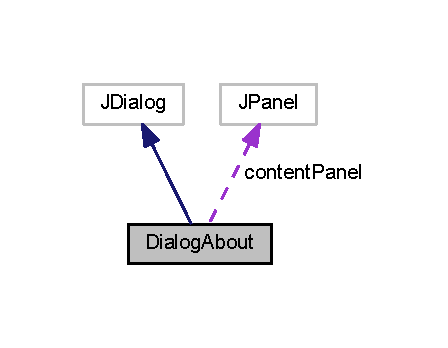
\includegraphics[width=215pt]{classcom_1_1lclion_1_1midigui_1_1_dialog_about__coll__graph}
\end{center}
\end{figure}
\subsection*{Public Member Functions}
\begin{DoxyCompactItemize}
\item 
\hyperlink{classcom_1_1lclion_1_1midigui_1_1_dialog_about_ae16533b3b532405ec4d2aea64d0ff351}{Dialog\+About} (J\+Frame parent)
\end{DoxyCompactItemize}
\subsection*{Private Attributes}
\begin{DoxyCompactItemize}
\item 
final J\+Panel \hyperlink{classcom_1_1lclion_1_1midigui_1_1_dialog_about_ac383c7b38c74b9e1cc245a00de4fbb5e}{content\+Panel} = new J\+Panel()
\begin{DoxyCompactList}\small\item\em A content panel that stores various components. \end{DoxyCompactList}\end{DoxyCompactItemize}


\subsection{Detailed Description}
A dialog showing software information. 

Java Swing components used to render text and images in this dialog is declared locally in constructor, refer to source code for component details. \begin{DoxyAuthor}{Author}
L\+C Lion 
\end{DoxyAuthor}


\subsection{Constructor \& Destructor Documentation}
\hypertarget{classcom_1_1lclion_1_1midigui_1_1_dialog_about_ae16533b3b532405ec4d2aea64d0ff351}{\index{com\+::lclion\+::midigui\+::\+Dialog\+About@{com\+::lclion\+::midigui\+::\+Dialog\+About}!Dialog\+About@{Dialog\+About}}
\index{Dialog\+About@{Dialog\+About}!com\+::lclion\+::midigui\+::\+Dialog\+About@{com\+::lclion\+::midigui\+::\+Dialog\+About}}
\subsubsection[{Dialog\+About}]{\setlength{\rightskip}{0pt plus 5cm}{\bf Dialog\+About} (
\begin{DoxyParamCaption}
\item[{J\+Frame}]{parent}
\end{DoxyParamCaption}
)}}\label{classcom_1_1lclion_1_1midigui_1_1_dialog_about_ae16533b3b532405ec4d2aea64d0ff351}
Create the dialog. Initialises Java Swing Components that may not be displayed on the Collaboration diagram as it is declared in local scope. 
\begin{DoxyParams}{Parameters}
{\em parent} & The parent of this dialog. Used to set the dialog relative to it's parent. \\
\hline
\end{DoxyParams}


\subsection{Member Data Documentation}
\hypertarget{classcom_1_1lclion_1_1midigui_1_1_dialog_about_ac383c7b38c74b9e1cc245a00de4fbb5e}{\index{com\+::lclion\+::midigui\+::\+Dialog\+About@{com\+::lclion\+::midigui\+::\+Dialog\+About}!content\+Panel@{content\+Panel}}
\index{content\+Panel@{content\+Panel}!com\+::lclion\+::midigui\+::\+Dialog\+About@{com\+::lclion\+::midigui\+::\+Dialog\+About}}
\subsubsection[{content\+Panel}]{\setlength{\rightskip}{0pt plus 5cm}final J\+Panel content\+Panel = new J\+Panel()\hspace{0.3cm}{\ttfamily [private]}}}\label{classcom_1_1lclion_1_1midigui_1_1_dialog_about_ac383c7b38c74b9e1cc245a00de4fbb5e}


A content panel that stores various components. 



The documentation for this class was generated from the following file\+:\begin{DoxyCompactItemize}
\item 
src/com/lclion/midigui/\hyperlink{_dialog_about_8java}{Dialog\+About.\+java}\end{DoxyCompactItemize}

\hypertarget{classcom_1_1lclion_1_1midigui_1_1_dialog_colour_reference}{\section{Dialog\+Colour\+Reference Class Reference}
\label{classcom_1_1lclion_1_1midigui_1_1_dialog_colour_reference}\index{Dialog\+Colour\+Reference@{Dialog\+Colour\+Reference}}
}


A dialog that shows the note values in colour for users to use as reference.  




Collaboration diagram for Dialog\+Colour\+Reference\+:\nopagebreak
\begin{figure}[H]
\begin{center}
\leavevmode
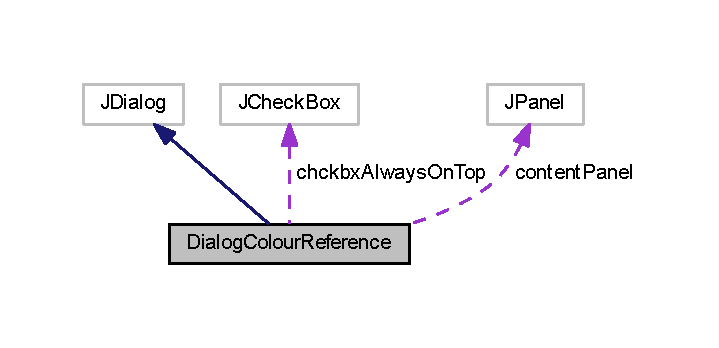
\includegraphics[width=345pt]{classcom_1_1lclion_1_1midigui_1_1_dialog_colour_reference__coll__graph}
\end{center}
\end{figure}
\subsection*{Public Member Functions}
\begin{DoxyCompactItemize}
\item 
\hyperlink{classcom_1_1lclion_1_1midigui_1_1_dialog_colour_reference_ae98709ca14db48a02783451719e792eb}{Dialog\+Colour\+Reference} (final J\+Frame parent)
\end{DoxyCompactItemize}
\subsection*{Private Attributes}
\begin{DoxyCompactItemize}
\item 
final J\+Panel \hyperlink{classcom_1_1lclion_1_1midigui_1_1_dialog_colour_reference_ac383c7b38c74b9e1cc245a00de4fbb5e}{content\+Panel} = new J\+Panel()
\item 
J\+Check\+Box \hyperlink{classcom_1_1lclion_1_1midigui_1_1_dialog_colour_reference_afb212360a6ff5330b0ca37ea40c372a8}{chckbx\+Always\+On\+Top}
\end{DoxyCompactItemize}


\subsection{Detailed Description}
A dialog that shows the note values in colour for users to use as reference. 

\begin{DoxyAuthor}{Author}
L\+C Lion 
\end{DoxyAuthor}


\subsection{Constructor \& Destructor Documentation}
\hypertarget{classcom_1_1lclion_1_1midigui_1_1_dialog_colour_reference_ae98709ca14db48a02783451719e792eb}{\index{com\+::lclion\+::midigui\+::\+Dialog\+Colour\+Reference@{com\+::lclion\+::midigui\+::\+Dialog\+Colour\+Reference}!Dialog\+Colour\+Reference@{Dialog\+Colour\+Reference}}
\index{Dialog\+Colour\+Reference@{Dialog\+Colour\+Reference}!com\+::lclion\+::midigui\+::\+Dialog\+Colour\+Reference@{com\+::lclion\+::midigui\+::\+Dialog\+Colour\+Reference}}
\subsubsection[{Dialog\+Colour\+Reference}]{\setlength{\rightskip}{0pt plus 5cm}{\bf Dialog\+Colour\+Reference} (
\begin{DoxyParamCaption}
\item[{final J\+Frame}]{parent}
\end{DoxyParamCaption}
)}}\label{classcom_1_1lclion_1_1midigui_1_1_dialog_colour_reference_ae98709ca14db48a02783451719e792eb}
Create the Colour Reference dialog. 

\subsection{Member Data Documentation}
\hypertarget{classcom_1_1lclion_1_1midigui_1_1_dialog_colour_reference_afb212360a6ff5330b0ca37ea40c372a8}{\index{com\+::lclion\+::midigui\+::\+Dialog\+Colour\+Reference@{com\+::lclion\+::midigui\+::\+Dialog\+Colour\+Reference}!chckbx\+Always\+On\+Top@{chckbx\+Always\+On\+Top}}
\index{chckbx\+Always\+On\+Top@{chckbx\+Always\+On\+Top}!com\+::lclion\+::midigui\+::\+Dialog\+Colour\+Reference@{com\+::lclion\+::midigui\+::\+Dialog\+Colour\+Reference}}
\subsubsection[{chckbx\+Always\+On\+Top}]{\setlength{\rightskip}{0pt plus 5cm}J\+Check\+Box chckbx\+Always\+On\+Top\hspace{0.3cm}{\ttfamily [private]}}}\label{classcom_1_1lclion_1_1midigui_1_1_dialog_colour_reference_afb212360a6ff5330b0ca37ea40c372a8}
\hypertarget{classcom_1_1lclion_1_1midigui_1_1_dialog_colour_reference_ac383c7b38c74b9e1cc245a00de4fbb5e}{\index{com\+::lclion\+::midigui\+::\+Dialog\+Colour\+Reference@{com\+::lclion\+::midigui\+::\+Dialog\+Colour\+Reference}!content\+Panel@{content\+Panel}}
\index{content\+Panel@{content\+Panel}!com\+::lclion\+::midigui\+::\+Dialog\+Colour\+Reference@{com\+::lclion\+::midigui\+::\+Dialog\+Colour\+Reference}}
\subsubsection[{content\+Panel}]{\setlength{\rightskip}{0pt plus 5cm}final J\+Panel content\+Panel = new J\+Panel()\hspace{0.3cm}{\ttfamily [private]}}}\label{classcom_1_1lclion_1_1midigui_1_1_dialog_colour_reference_ac383c7b38c74b9e1cc245a00de4fbb5e}


The documentation for this class was generated from the following file\+:\begin{DoxyCompactItemize}
\item 
src/com/lclion/midigui/\hyperlink{_dialog_colour_reference_8java}{Dialog\+Colour\+Reference.\+java}\end{DoxyCompactItemize}

\hypertarget{classcom_1_1lclion_1_1midigui_1_1_dialog_on_screen_keyboard}{\section{Dialog\+On\+Screen\+Keyboard Class Reference}
\label{classcom_1_1lclion_1_1midigui_1_1_dialog_on_screen_keyboard}\index{Dialog\+On\+Screen\+Keyboard@{Dialog\+On\+Screen\+Keyboard}}
}


Displays a preview of a Q\+W\+E\+R\+T\+Y keyboard, indicating the current note played from the main window.  




Collaboration diagram for Dialog\+On\+Screen\+Keyboard\+:\nopagebreak
\begin{figure}[H]
\begin{center}
\leavevmode
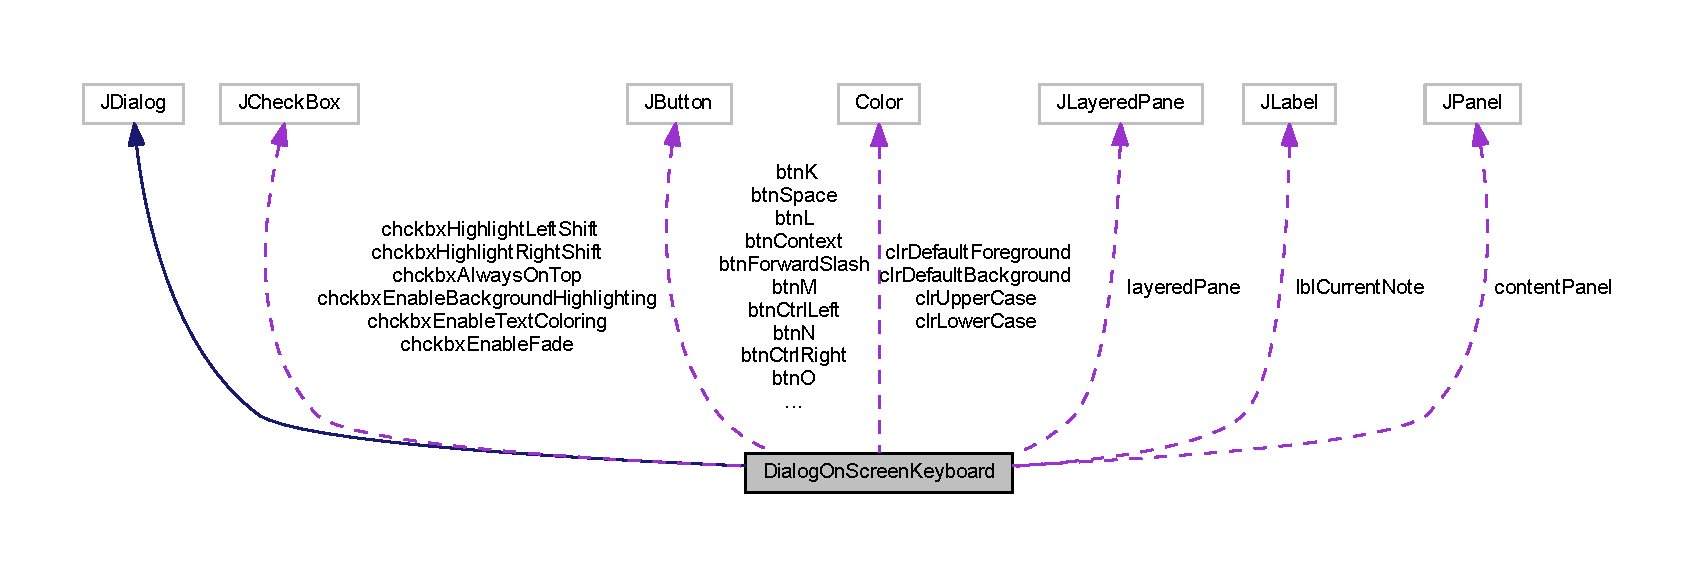
\includegraphics[width=350pt]{classcom_1_1lclion_1_1midigui_1_1_dialog_on_screen_keyboard__coll__graph}
\end{center}
\end{figure}
\subsection*{Public Member Functions}
\begin{DoxyCompactItemize}
\item 
\hyperlink{classcom_1_1lclion_1_1midigui_1_1_dialog_on_screen_keyboard_ac5f684ded8b7d9c9bb8f3fef7d5f6ebc}{Dialog\+On\+Screen\+Keyboard} (final J\+Frame parent)
\item 
void \hyperlink{classcom_1_1lclion_1_1midigui_1_1_dialog_on_screen_keyboard_ae11e61d422e0ffcfde71c2c8d22e8125}{highlight\+Keys} (String keys\+To\+Highlight)
\item 
void \hyperlink{classcom_1_1lclion_1_1midigui_1_1_dialog_on_screen_keyboard_aa6b620d240a70e879d6c4c94c2cddadf}{set\+Text} (String parsed\+Data)
\end{DoxyCompactItemize}
\subsection*{Private Member Functions}
\begin{DoxyCompactItemize}
\item 
void \hyperlink{classcom_1_1lclion_1_1midigui_1_1_dialog_on_screen_keyboard_ae91f8f91ce33c821d70b3d5e09c08cc7}{update\+Current\+Note\+Label} (String current\+Note)
\item 
void \hyperlink{classcom_1_1lclion_1_1midigui_1_1_dialog_on_screen_keyboard_ae2176f8320d6a67ec81ce53e3b0df321}{clear\+Highlights} ()
\item 
void \hyperlink{classcom_1_1lclion_1_1midigui_1_1_dialog_on_screen_keyboard_a8bb16dd8ea1ccc12b8032d397ab8b3e9}{toggle\+Components} (J\+Layered\+Pane container, boolean enable)
\end{DoxyCompactItemize}
\subsection*{Private Attributes}
\begin{DoxyCompactItemize}
\item 
int \hyperlink{classcom_1_1lclion_1_1midigui_1_1_dialog_on_screen_keyboard_a78dc3704e7e01da52c9a93a70c5bc45d}{font\+Size} = 14
\item 
int \hyperlink{classcom_1_1lclion_1_1midigui_1_1_dialog_on_screen_keyboard_aec4029056965b8b1d9e30178aa258e71}{font\+Style} = Font.\+B\+O\+L\+D
\item 
String \hyperlink{classcom_1_1lclion_1_1midigui_1_1_dialog_on_screen_keyboard_ab0f8a5a46d90946fe20e323cbc10384f}{font\+Family} = \char`\"{}Tahoma\char`\"{}
\item 
Color \hyperlink{classcom_1_1lclion_1_1midigui_1_1_dialog_on_screen_keyboard_a6213a3fc55162f385ecf68112b98d6cf}{clr\+Lower\+Case} = new Color(0, 153, 0)
\item 
Color \hyperlink{classcom_1_1lclion_1_1midigui_1_1_dialog_on_screen_keyboard_a18bfeb811deb62b61ddeb555174ca785}{clr\+Upper\+Case} = new Color(255, 0, 0)
\item 
Color \hyperlink{classcom_1_1lclion_1_1midigui_1_1_dialog_on_screen_keyboard_a07f32e805fc4b2bb4953e4fc63ac0c3c}{clr\+Default\+Background} = new Color(255, 255, 255)
\item 
Color \hyperlink{classcom_1_1lclion_1_1midigui_1_1_dialog_on_screen_keyboard_aa8736f6d433f5918da7935630e4491d9}{clr\+Default\+Foreground} = new Color(255, 255, 255)
\item 
final J\+Panel \hyperlink{classcom_1_1lclion_1_1midigui_1_1_dialog_on_screen_keyboard_ac383c7b38c74b9e1cc245a00de4fbb5e}{content\+Panel} = new J\+Panel()
\item 
J\+Layered\+Pane \hyperlink{classcom_1_1lclion_1_1midigui_1_1_dialog_on_screen_keyboard_a90de2803c72845b70771d7326d038f45}{layered\+Pane}
\item 
J\+Button \hyperlink{classcom_1_1lclion_1_1midigui_1_1_dialog_on_screen_keyboard_a2d7738272489586031bc93d39302aed9}{btn\+Tilda}
\item 
J\+Button \hyperlink{classcom_1_1lclion_1_1midigui_1_1_dialog_on_screen_keyboard_a2c3163c016e15ebbb4071599c1d15029}{btn1}
\item 
J\+Button \hyperlink{classcom_1_1lclion_1_1midigui_1_1_dialog_on_screen_keyboard_aa093c8b4f751c9c929117324fb2ccb0c}{btn2}
\item 
J\+Button \hyperlink{classcom_1_1lclion_1_1midigui_1_1_dialog_on_screen_keyboard_aaff3703d264eab6c3f736790b6535faa}{btn3}
\item 
J\+Button \hyperlink{classcom_1_1lclion_1_1midigui_1_1_dialog_on_screen_keyboard_ac426d68c2e7a84c6b7ce057c1be96f74}{btn4}
\item 
J\+Button \hyperlink{classcom_1_1lclion_1_1midigui_1_1_dialog_on_screen_keyboard_a6987bceedd9d1cadf7b24b1426f4ffd6}{btn5}
\item 
J\+Button \hyperlink{classcom_1_1lclion_1_1midigui_1_1_dialog_on_screen_keyboard_ae94729859505651df0186afd93a55f3a}{btn6}
\item 
J\+Button \hyperlink{classcom_1_1lclion_1_1midigui_1_1_dialog_on_screen_keyboard_a8cce3d18dfb219ac20321fd0f66ac21c}{btn7}
\item 
J\+Button \hyperlink{classcom_1_1lclion_1_1midigui_1_1_dialog_on_screen_keyboard_aa781873bcc563594efcf281a6196e52f}{btn8}
\item 
J\+Button \hyperlink{classcom_1_1lclion_1_1midigui_1_1_dialog_on_screen_keyboard_a22c8181bc00931a15d201154c28c0aff}{btn9}
\item 
J\+Button \hyperlink{classcom_1_1lclion_1_1midigui_1_1_dialog_on_screen_keyboard_a38cfd1e15e0f3542b16c4b3e413df733}{btn0}
\item 
J\+Button \hyperlink{classcom_1_1lclion_1_1midigui_1_1_dialog_on_screen_keyboard_ad781fc7a840a15bb7c7707d1d909176a}{btn\+Tab}
\item 
J\+Button \hyperlink{classcom_1_1lclion_1_1midigui_1_1_dialog_on_screen_keyboard_a57bb93658a349e6c2ecf7be5811869c4}{btn\+Q}
\item 
J\+Button \hyperlink{classcom_1_1lclion_1_1midigui_1_1_dialog_on_screen_keyboard_a95f5495566cf1ce41a3dcdeecf4ec242}{btn\+W}
\item 
J\+Button \hyperlink{classcom_1_1lclion_1_1midigui_1_1_dialog_on_screen_keyboard_aab5a0eb82195c831ebdd86b721d70d2f}{btn\+E}
\item 
J\+Button \hyperlink{classcom_1_1lclion_1_1midigui_1_1_dialog_on_screen_keyboard_ad203cb9fabff2fe0e0768dc8b347f84d}{btn\+R}
\item 
J\+Button \hyperlink{classcom_1_1lclion_1_1midigui_1_1_dialog_on_screen_keyboard_ad28bed9f4636752c166720536df81332}{btn\+T}
\item 
J\+Button \hyperlink{classcom_1_1lclion_1_1midigui_1_1_dialog_on_screen_keyboard_ae08fc1d8a7a3aadb9c5a3a3961495839}{btn\+U}
\item 
J\+Button \hyperlink{classcom_1_1lclion_1_1midigui_1_1_dialog_on_screen_keyboard_a97c660d9d6bdd8feb471d8fc5c7db2c0}{btn\+I}
\item 
J\+Button \hyperlink{classcom_1_1lclion_1_1midigui_1_1_dialog_on_screen_keyboard_a73a3757d23cd3530b13b3d13629874cf}{btn\+O}
\item 
J\+Button \hyperlink{classcom_1_1lclion_1_1midigui_1_1_dialog_on_screen_keyboard_a1dfa67c9987734db4c0042b092fed42c}{btn\+P}
\item 
J\+Button \hyperlink{classcom_1_1lclion_1_1midigui_1_1_dialog_on_screen_keyboard_ac209a6c2fffe7ac528b96eed8e8580d5}{btn\+Y}
\item 
J\+Button \hyperlink{classcom_1_1lclion_1_1midigui_1_1_dialog_on_screen_keyboard_ad837540dd78a68fa4a9de57214bbd3d8}{btn\+Caps\+Lock}
\item 
J\+Button \hyperlink{classcom_1_1lclion_1_1midigui_1_1_dialog_on_screen_keyboard_a1e8b342c7fe8b296c098ddce1ae1d7b2}{btn\+A}
\item 
J\+Button \hyperlink{classcom_1_1lclion_1_1midigui_1_1_dialog_on_screen_keyboard_a054a67bc166a83efa481b49a6d6024eb}{btn\+S}
\item 
J\+Button \hyperlink{classcom_1_1lclion_1_1midigui_1_1_dialog_on_screen_keyboard_a89073807d2322dc0c1e5f828fbb76764}{btn\+D}
\item 
J\+Button \hyperlink{classcom_1_1lclion_1_1midigui_1_1_dialog_on_screen_keyboard_a64af979f8cb527c387b69ff58c4f1120}{btn\+F}
\item 
J\+Button \hyperlink{classcom_1_1lclion_1_1midigui_1_1_dialog_on_screen_keyboard_a87f9f3a6ee563233c354a5b39b9cc54a}{btn\+G}
\item 
J\+Button \hyperlink{classcom_1_1lclion_1_1midigui_1_1_dialog_on_screen_keyboard_a9531fabd22b34462f4a7918e72f60ac7}{btn\+J}
\item 
J\+Button \hyperlink{classcom_1_1lclion_1_1midigui_1_1_dialog_on_screen_keyboard_a1fabae8535d894d70bde32a11be3d376}{btn\+K}
\item 
J\+Button \hyperlink{classcom_1_1lclion_1_1midigui_1_1_dialog_on_screen_keyboard_a79e6c03d54b3d704811e7c9e4c67d5d2}{btn\+L}
\item 
J\+Button \hyperlink{classcom_1_1lclion_1_1midigui_1_1_dialog_on_screen_keyboard_ab44b089f992b314233069b2d53a2fc54}{btn\+H}
\item 
J\+Button \hyperlink{classcom_1_1lclion_1_1midigui_1_1_dialog_on_screen_keyboard_a0a16dbfc7b21d8782aefcfb5b11e4ce8}{btn\+Shift\+Left}
\item 
J\+Button \hyperlink{classcom_1_1lclion_1_1midigui_1_1_dialog_on_screen_keyboard_aa22f6a6fb7a890cd8ec5022973c923ea}{btn\+Z}
\item 
J\+Button \hyperlink{classcom_1_1lclion_1_1midigui_1_1_dialog_on_screen_keyboard_a17e4aaf74e496f1708a8996ad6f9168f}{btn\+X}
\item 
J\+Button \hyperlink{classcom_1_1lclion_1_1midigui_1_1_dialog_on_screen_keyboard_a108c048ae6e4a0db145ee98ea9df481f}{btn\+C}
\item 
J\+Button \hyperlink{classcom_1_1lclion_1_1midigui_1_1_dialog_on_screen_keyboard_aadd7043de06b30089cb9b8ca0943a5ea}{btn\+V}
\item 
J\+Button \hyperlink{classcom_1_1lclion_1_1midigui_1_1_dialog_on_screen_keyboard_a34a37d547948df48303ba0103cde59de}{btn\+B}
\item 
J\+Button \hyperlink{classcom_1_1lclion_1_1midigui_1_1_dialog_on_screen_keyboard_af47ad194bb3c4931c47c17f5d9ec98c4}{btn\+M}
\item 
J\+Button \hyperlink{classcom_1_1lclion_1_1midigui_1_1_dialog_on_screen_keyboard_a99f24b18e5f535f5666b073fe414fdfa}{btn\+N}
\item 
J\+Check\+Box \hyperlink{classcom_1_1lclion_1_1midigui_1_1_dialog_on_screen_keyboard_a9aaed51dba7caa44dc53b28e7acc096d}{chckbx\+Highlight\+Left\+Shift}
\item 
J\+Check\+Box \hyperlink{classcom_1_1lclion_1_1midigui_1_1_dialog_on_screen_keyboard_a8dd6d82143f4aedba6236c67bf6c733f}{chckbx\+Enable\+Fade}
\item 
J\+Button \hyperlink{classcom_1_1lclion_1_1midigui_1_1_dialog_on_screen_keyboard_a5d7ba779d4e74df2616b1a5fb6fdbdfd}{btn\+Minus}
\item 
J\+Button \hyperlink{classcom_1_1lclion_1_1midigui_1_1_dialog_on_screen_keyboard_aeccc007709a2413953c476a47633484d}{btn\+Equal}
\item 
J\+Button \hyperlink{classcom_1_1lclion_1_1midigui_1_1_dialog_on_screen_keyboard_af531e3a095c123589a66fc5aa9373067}{btn\+Backspace}
\item 
J\+Button \hyperlink{classcom_1_1lclion_1_1midigui_1_1_dialog_on_screen_keyboard_ad6c00cf5c5a45173be827dafa072041b}{btn\+Square\+Bracket\+Open}
\item 
J\+Button \hyperlink{classcom_1_1lclion_1_1midigui_1_1_dialog_on_screen_keyboard_a35b8fdc6e8d3dd6062dc18572df13e7d}{btn\+Square\+Bracket\+Close}
\item 
J\+Button \hyperlink{classcom_1_1lclion_1_1midigui_1_1_dialog_on_screen_keyboard_afcc98561cbf032feebf7b1538b1ba688}{btn\+Backslash}
\item 
J\+Button \hyperlink{classcom_1_1lclion_1_1midigui_1_1_dialog_on_screen_keyboard_afbc77b1edd4a0583a8e7699a9f15ded7}{btn\+Semicolon}
\item 
J\+Button \hyperlink{classcom_1_1lclion_1_1midigui_1_1_dialog_on_screen_keyboard_af8bd4bb6dd42d1f0c8b9432a7b3dd5e5}{btn\+Apostraphe}
\item 
J\+Button \hyperlink{classcom_1_1lclion_1_1midigui_1_1_dialog_on_screen_keyboard_ad7ed480b341e2e453e5857f54f2c0574}{btn\+Enter}
\item 
J\+Button \hyperlink{classcom_1_1lclion_1_1midigui_1_1_dialog_on_screen_keyboard_a78351a2292cd2bb5e405a7fb63bde8da}{btn\+Comma}
\item 
J\+Button \hyperlink{classcom_1_1lclion_1_1midigui_1_1_dialog_on_screen_keyboard_a4d5afe8ca2d30a690e44801559516daa}{btn\+Full\+Stop}
\item 
J\+Button \hyperlink{classcom_1_1lclion_1_1midigui_1_1_dialog_on_screen_keyboard_afc4fa10ed9a8c74b5ba3976b0f9513ef}{btn\+Forward\+Slash}
\item 
J\+Button \hyperlink{classcom_1_1lclion_1_1midigui_1_1_dialog_on_screen_keyboard_ae375d25d5103fe59e93bfe78bf894722}{btn\+Shift\+Right}
\item 
J\+Button \hyperlink{classcom_1_1lclion_1_1midigui_1_1_dialog_on_screen_keyboard_a79eb966f6f33a2cd4f9d46cd50a7d480}{btn\+Ctrl\+Left}
\item 
J\+Button \hyperlink{classcom_1_1lclion_1_1midigui_1_1_dialog_on_screen_keyboard_a1f5a6207904a8e20962cd520ea141d9b}{btn\+Win\+Left}
\item 
J\+Button \hyperlink{classcom_1_1lclion_1_1midigui_1_1_dialog_on_screen_keyboard_ae9d61f4815d45ac8888e4a7bf4344cc1}{btn\+Alt\+Left}
\item 
J\+Button \hyperlink{classcom_1_1lclion_1_1midigui_1_1_dialog_on_screen_keyboard_a5bffdd7e1b028002ae5b5464a4a289b9}{btn\+Space}
\item 
J\+Button \hyperlink{classcom_1_1lclion_1_1midigui_1_1_dialog_on_screen_keyboard_a3deb641d54b510ef4243b41c235d7d26}{btn\+Alt\+Right}
\item 
J\+Button \hyperlink{classcom_1_1lclion_1_1midigui_1_1_dialog_on_screen_keyboard_a7820654d38a637ac4cc0150639d8f99e}{btn\+Win\+Right}
\item 
J\+Button \hyperlink{classcom_1_1lclion_1_1midigui_1_1_dialog_on_screen_keyboard_a3aaad9ec5791601fbc2c85c6c87e73de}{btn\+Context}
\item 
J\+Button \hyperlink{classcom_1_1lclion_1_1midigui_1_1_dialog_on_screen_keyboard_aaa66232d265147ac72c937bf5569bacc}{btn\+Ctrl\+Right}
\item 
J\+Check\+Box \hyperlink{classcom_1_1lclion_1_1midigui_1_1_dialog_on_screen_keyboard_a439f5c81e352809a4343216fbaf9a5c8}{chckbx\+Highlight\+Right\+Shift}
\item 
J\+Check\+Box \hyperlink{classcom_1_1lclion_1_1midigui_1_1_dialog_on_screen_keyboard_ad4773803d6cd9e0515570c744f580f20}{chckbx\+Enable\+Text\+Coloring}
\item 
J\+Check\+Box \hyperlink{classcom_1_1lclion_1_1midigui_1_1_dialog_on_screen_keyboard_a6b0daa2762d684f43a1ef4e4aaca718d}{chckbx\+Enable\+Background\+Highlighting}
\item 
J\+Label \hyperlink{classcom_1_1lclion_1_1midigui_1_1_dialog_on_screen_keyboard_a97722586d2e85bb697b3512b1fcbf729}{lbl\+Current\+Note}
\item 
J\+Check\+Box \hyperlink{classcom_1_1lclion_1_1midigui_1_1_dialog_on_screen_keyboard_afb212360a6ff5330b0ca37ea40c372a8}{chckbx\+Always\+On\+Top}
\end{DoxyCompactItemize}


\subsection{Detailed Description}
Displays a preview of a Q\+W\+E\+R\+T\+Y keyboard, indicating the current note played from the main window. 

\begin{DoxyAuthor}{Author}
L\+C Lion 
\end{DoxyAuthor}


\subsection{Constructor \& Destructor Documentation}
\hypertarget{classcom_1_1lclion_1_1midigui_1_1_dialog_on_screen_keyboard_ac5f684ded8b7d9c9bb8f3fef7d5f6ebc}{\index{com\+::lclion\+::midigui\+::\+Dialog\+On\+Screen\+Keyboard@{com\+::lclion\+::midigui\+::\+Dialog\+On\+Screen\+Keyboard}!Dialog\+On\+Screen\+Keyboard@{Dialog\+On\+Screen\+Keyboard}}
\index{Dialog\+On\+Screen\+Keyboard@{Dialog\+On\+Screen\+Keyboard}!com\+::lclion\+::midigui\+::\+Dialog\+On\+Screen\+Keyboard@{com\+::lclion\+::midigui\+::\+Dialog\+On\+Screen\+Keyboard}}
\subsubsection[{Dialog\+On\+Screen\+Keyboard}]{\setlength{\rightskip}{0pt plus 5cm}{\bf Dialog\+On\+Screen\+Keyboard} (
\begin{DoxyParamCaption}
\item[{final J\+Frame}]{parent}
\end{DoxyParamCaption}
)}}\label{classcom_1_1lclion_1_1midigui_1_1_dialog_on_screen_keyboard_ac5f684ded8b7d9c9bb8f3fef7d5f6ebc}
Create the dialog. 

Here is the call graph for this function\+:\nopagebreak
\begin{figure}[H]
\begin{center}
\leavevmode
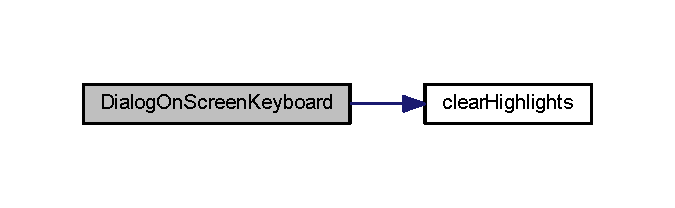
\includegraphics[width=324pt]{classcom_1_1lclion_1_1midigui_1_1_dialog_on_screen_keyboard_ac5f684ded8b7d9c9bb8f3fef7d5f6ebc_cgraph}
\end{center}
\end{figure}




\subsection{Member Function Documentation}
\hypertarget{classcom_1_1lclion_1_1midigui_1_1_dialog_on_screen_keyboard_ae2176f8320d6a67ec81ce53e3b0df321}{\index{com\+::lclion\+::midigui\+::\+Dialog\+On\+Screen\+Keyboard@{com\+::lclion\+::midigui\+::\+Dialog\+On\+Screen\+Keyboard}!clear\+Highlights@{clear\+Highlights}}
\index{clear\+Highlights@{clear\+Highlights}!com\+::lclion\+::midigui\+::\+Dialog\+On\+Screen\+Keyboard@{com\+::lclion\+::midigui\+::\+Dialog\+On\+Screen\+Keyboard}}
\subsubsection[{clear\+Highlights}]{\setlength{\rightskip}{0pt plus 5cm}void clear\+Highlights (
\begin{DoxyParamCaption}
{}
\end{DoxyParamCaption}
)\hspace{0.3cm}{\ttfamily [private]}}}\label{classcom_1_1lclion_1_1midigui_1_1_dialog_on_screen_keyboard_ae2176f8320d6a67ec81ce53e3b0df321}
\hypertarget{classcom_1_1lclion_1_1midigui_1_1_dialog_on_screen_keyboard_ae11e61d422e0ffcfde71c2c8d22e8125}{\index{com\+::lclion\+::midigui\+::\+Dialog\+On\+Screen\+Keyboard@{com\+::lclion\+::midigui\+::\+Dialog\+On\+Screen\+Keyboard}!highlight\+Keys@{highlight\+Keys}}
\index{highlight\+Keys@{highlight\+Keys}!com\+::lclion\+::midigui\+::\+Dialog\+On\+Screen\+Keyboard@{com\+::lclion\+::midigui\+::\+Dialog\+On\+Screen\+Keyboard}}
\subsubsection[{highlight\+Keys}]{\setlength{\rightskip}{0pt plus 5cm}void highlight\+Keys (
\begin{DoxyParamCaption}
\item[{String}]{keys\+To\+Highlight}
\end{DoxyParamCaption}
)}}\label{classcom_1_1lclion_1_1midigui_1_1_dialog_on_screen_keyboard_ae11e61d422e0ffcfde71c2c8d22e8125}


Here is the call graph for this function\+:\nopagebreak
\begin{figure}[H]
\begin{center}
\leavevmode
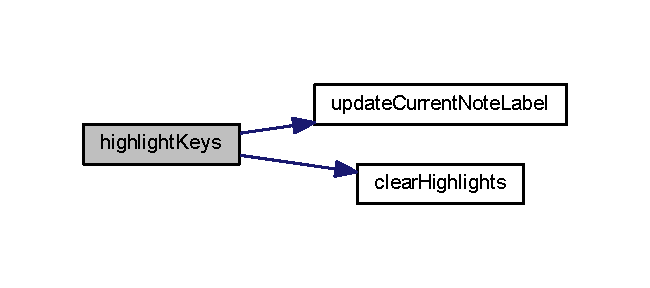
\includegraphics[width=312pt]{classcom_1_1lclion_1_1midigui_1_1_dialog_on_screen_keyboard_ae11e61d422e0ffcfde71c2c8d22e8125_cgraph}
\end{center}
\end{figure}


\hypertarget{classcom_1_1lclion_1_1midigui_1_1_dialog_on_screen_keyboard_aa6b620d240a70e879d6c4c94c2cddadf}{\index{com\+::lclion\+::midigui\+::\+Dialog\+On\+Screen\+Keyboard@{com\+::lclion\+::midigui\+::\+Dialog\+On\+Screen\+Keyboard}!set\+Text@{set\+Text}}
\index{set\+Text@{set\+Text}!com\+::lclion\+::midigui\+::\+Dialog\+On\+Screen\+Keyboard@{com\+::lclion\+::midigui\+::\+Dialog\+On\+Screen\+Keyboard}}
\subsubsection[{set\+Text}]{\setlength{\rightskip}{0pt plus 5cm}void set\+Text (
\begin{DoxyParamCaption}
\item[{String}]{parsed\+Data}
\end{DoxyParamCaption}
)}}\label{classcom_1_1lclion_1_1midigui_1_1_dialog_on_screen_keyboard_aa6b620d240a70e879d6c4c94c2cddadf}
\hypertarget{classcom_1_1lclion_1_1midigui_1_1_dialog_on_screen_keyboard_a8bb16dd8ea1ccc12b8032d397ab8b3e9}{\index{com\+::lclion\+::midigui\+::\+Dialog\+On\+Screen\+Keyboard@{com\+::lclion\+::midigui\+::\+Dialog\+On\+Screen\+Keyboard}!toggle\+Components@{toggle\+Components}}
\index{toggle\+Components@{toggle\+Components}!com\+::lclion\+::midigui\+::\+Dialog\+On\+Screen\+Keyboard@{com\+::lclion\+::midigui\+::\+Dialog\+On\+Screen\+Keyboard}}
\subsubsection[{toggle\+Components}]{\setlength{\rightskip}{0pt plus 5cm}void toggle\+Components (
\begin{DoxyParamCaption}
\item[{J\+Layered\+Pane}]{container, }
\item[{boolean}]{enable}
\end{DoxyParamCaption}
)\hspace{0.3cm}{\ttfamily [private]}}}\label{classcom_1_1lclion_1_1midigui_1_1_dialog_on_screen_keyboard_a8bb16dd8ea1ccc12b8032d397ab8b3e9}
\hypertarget{classcom_1_1lclion_1_1midigui_1_1_dialog_on_screen_keyboard_ae91f8f91ce33c821d70b3d5e09c08cc7}{\index{com\+::lclion\+::midigui\+::\+Dialog\+On\+Screen\+Keyboard@{com\+::lclion\+::midigui\+::\+Dialog\+On\+Screen\+Keyboard}!update\+Current\+Note\+Label@{update\+Current\+Note\+Label}}
\index{update\+Current\+Note\+Label@{update\+Current\+Note\+Label}!com\+::lclion\+::midigui\+::\+Dialog\+On\+Screen\+Keyboard@{com\+::lclion\+::midigui\+::\+Dialog\+On\+Screen\+Keyboard}}
\subsubsection[{update\+Current\+Note\+Label}]{\setlength{\rightskip}{0pt plus 5cm}void update\+Current\+Note\+Label (
\begin{DoxyParamCaption}
\item[{String}]{current\+Note}
\end{DoxyParamCaption}
)\hspace{0.3cm}{\ttfamily [private]}}}\label{classcom_1_1lclion_1_1midigui_1_1_dialog_on_screen_keyboard_ae91f8f91ce33c821d70b3d5e09c08cc7}


\subsection{Member Data Documentation}
\hypertarget{classcom_1_1lclion_1_1midigui_1_1_dialog_on_screen_keyboard_a38cfd1e15e0f3542b16c4b3e413df733}{\index{com\+::lclion\+::midigui\+::\+Dialog\+On\+Screen\+Keyboard@{com\+::lclion\+::midigui\+::\+Dialog\+On\+Screen\+Keyboard}!btn0@{btn0}}
\index{btn0@{btn0}!com\+::lclion\+::midigui\+::\+Dialog\+On\+Screen\+Keyboard@{com\+::lclion\+::midigui\+::\+Dialog\+On\+Screen\+Keyboard}}
\subsubsection[{btn0}]{\setlength{\rightskip}{0pt plus 5cm}J\+Button btn0\hspace{0.3cm}{\ttfamily [private]}}}\label{classcom_1_1lclion_1_1midigui_1_1_dialog_on_screen_keyboard_a38cfd1e15e0f3542b16c4b3e413df733}
\hypertarget{classcom_1_1lclion_1_1midigui_1_1_dialog_on_screen_keyboard_a2c3163c016e15ebbb4071599c1d15029}{\index{com\+::lclion\+::midigui\+::\+Dialog\+On\+Screen\+Keyboard@{com\+::lclion\+::midigui\+::\+Dialog\+On\+Screen\+Keyboard}!btn1@{btn1}}
\index{btn1@{btn1}!com\+::lclion\+::midigui\+::\+Dialog\+On\+Screen\+Keyboard@{com\+::lclion\+::midigui\+::\+Dialog\+On\+Screen\+Keyboard}}
\subsubsection[{btn1}]{\setlength{\rightskip}{0pt plus 5cm}J\+Button btn1\hspace{0.3cm}{\ttfamily [private]}}}\label{classcom_1_1lclion_1_1midigui_1_1_dialog_on_screen_keyboard_a2c3163c016e15ebbb4071599c1d15029}
\hypertarget{classcom_1_1lclion_1_1midigui_1_1_dialog_on_screen_keyboard_aa093c8b4f751c9c929117324fb2ccb0c}{\index{com\+::lclion\+::midigui\+::\+Dialog\+On\+Screen\+Keyboard@{com\+::lclion\+::midigui\+::\+Dialog\+On\+Screen\+Keyboard}!btn2@{btn2}}
\index{btn2@{btn2}!com\+::lclion\+::midigui\+::\+Dialog\+On\+Screen\+Keyboard@{com\+::lclion\+::midigui\+::\+Dialog\+On\+Screen\+Keyboard}}
\subsubsection[{btn2}]{\setlength{\rightskip}{0pt plus 5cm}J\+Button btn2\hspace{0.3cm}{\ttfamily [private]}}}\label{classcom_1_1lclion_1_1midigui_1_1_dialog_on_screen_keyboard_aa093c8b4f751c9c929117324fb2ccb0c}
\hypertarget{classcom_1_1lclion_1_1midigui_1_1_dialog_on_screen_keyboard_aaff3703d264eab6c3f736790b6535faa}{\index{com\+::lclion\+::midigui\+::\+Dialog\+On\+Screen\+Keyboard@{com\+::lclion\+::midigui\+::\+Dialog\+On\+Screen\+Keyboard}!btn3@{btn3}}
\index{btn3@{btn3}!com\+::lclion\+::midigui\+::\+Dialog\+On\+Screen\+Keyboard@{com\+::lclion\+::midigui\+::\+Dialog\+On\+Screen\+Keyboard}}
\subsubsection[{btn3}]{\setlength{\rightskip}{0pt plus 5cm}J\+Button btn3\hspace{0.3cm}{\ttfamily [private]}}}\label{classcom_1_1lclion_1_1midigui_1_1_dialog_on_screen_keyboard_aaff3703d264eab6c3f736790b6535faa}
\hypertarget{classcom_1_1lclion_1_1midigui_1_1_dialog_on_screen_keyboard_ac426d68c2e7a84c6b7ce057c1be96f74}{\index{com\+::lclion\+::midigui\+::\+Dialog\+On\+Screen\+Keyboard@{com\+::lclion\+::midigui\+::\+Dialog\+On\+Screen\+Keyboard}!btn4@{btn4}}
\index{btn4@{btn4}!com\+::lclion\+::midigui\+::\+Dialog\+On\+Screen\+Keyboard@{com\+::lclion\+::midigui\+::\+Dialog\+On\+Screen\+Keyboard}}
\subsubsection[{btn4}]{\setlength{\rightskip}{0pt plus 5cm}J\+Button btn4\hspace{0.3cm}{\ttfamily [private]}}}\label{classcom_1_1lclion_1_1midigui_1_1_dialog_on_screen_keyboard_ac426d68c2e7a84c6b7ce057c1be96f74}
\hypertarget{classcom_1_1lclion_1_1midigui_1_1_dialog_on_screen_keyboard_a6987bceedd9d1cadf7b24b1426f4ffd6}{\index{com\+::lclion\+::midigui\+::\+Dialog\+On\+Screen\+Keyboard@{com\+::lclion\+::midigui\+::\+Dialog\+On\+Screen\+Keyboard}!btn5@{btn5}}
\index{btn5@{btn5}!com\+::lclion\+::midigui\+::\+Dialog\+On\+Screen\+Keyboard@{com\+::lclion\+::midigui\+::\+Dialog\+On\+Screen\+Keyboard}}
\subsubsection[{btn5}]{\setlength{\rightskip}{0pt plus 5cm}J\+Button btn5\hspace{0.3cm}{\ttfamily [private]}}}\label{classcom_1_1lclion_1_1midigui_1_1_dialog_on_screen_keyboard_a6987bceedd9d1cadf7b24b1426f4ffd6}
\hypertarget{classcom_1_1lclion_1_1midigui_1_1_dialog_on_screen_keyboard_ae94729859505651df0186afd93a55f3a}{\index{com\+::lclion\+::midigui\+::\+Dialog\+On\+Screen\+Keyboard@{com\+::lclion\+::midigui\+::\+Dialog\+On\+Screen\+Keyboard}!btn6@{btn6}}
\index{btn6@{btn6}!com\+::lclion\+::midigui\+::\+Dialog\+On\+Screen\+Keyboard@{com\+::lclion\+::midigui\+::\+Dialog\+On\+Screen\+Keyboard}}
\subsubsection[{btn6}]{\setlength{\rightskip}{0pt plus 5cm}J\+Button btn6\hspace{0.3cm}{\ttfamily [private]}}}\label{classcom_1_1lclion_1_1midigui_1_1_dialog_on_screen_keyboard_ae94729859505651df0186afd93a55f3a}
\hypertarget{classcom_1_1lclion_1_1midigui_1_1_dialog_on_screen_keyboard_a8cce3d18dfb219ac20321fd0f66ac21c}{\index{com\+::lclion\+::midigui\+::\+Dialog\+On\+Screen\+Keyboard@{com\+::lclion\+::midigui\+::\+Dialog\+On\+Screen\+Keyboard}!btn7@{btn7}}
\index{btn7@{btn7}!com\+::lclion\+::midigui\+::\+Dialog\+On\+Screen\+Keyboard@{com\+::lclion\+::midigui\+::\+Dialog\+On\+Screen\+Keyboard}}
\subsubsection[{btn7}]{\setlength{\rightskip}{0pt plus 5cm}J\+Button btn7\hspace{0.3cm}{\ttfamily [private]}}}\label{classcom_1_1lclion_1_1midigui_1_1_dialog_on_screen_keyboard_a8cce3d18dfb219ac20321fd0f66ac21c}
\hypertarget{classcom_1_1lclion_1_1midigui_1_1_dialog_on_screen_keyboard_aa781873bcc563594efcf281a6196e52f}{\index{com\+::lclion\+::midigui\+::\+Dialog\+On\+Screen\+Keyboard@{com\+::lclion\+::midigui\+::\+Dialog\+On\+Screen\+Keyboard}!btn8@{btn8}}
\index{btn8@{btn8}!com\+::lclion\+::midigui\+::\+Dialog\+On\+Screen\+Keyboard@{com\+::lclion\+::midigui\+::\+Dialog\+On\+Screen\+Keyboard}}
\subsubsection[{btn8}]{\setlength{\rightskip}{0pt plus 5cm}J\+Button btn8\hspace{0.3cm}{\ttfamily [private]}}}\label{classcom_1_1lclion_1_1midigui_1_1_dialog_on_screen_keyboard_aa781873bcc563594efcf281a6196e52f}
\hypertarget{classcom_1_1lclion_1_1midigui_1_1_dialog_on_screen_keyboard_a22c8181bc00931a15d201154c28c0aff}{\index{com\+::lclion\+::midigui\+::\+Dialog\+On\+Screen\+Keyboard@{com\+::lclion\+::midigui\+::\+Dialog\+On\+Screen\+Keyboard}!btn9@{btn9}}
\index{btn9@{btn9}!com\+::lclion\+::midigui\+::\+Dialog\+On\+Screen\+Keyboard@{com\+::lclion\+::midigui\+::\+Dialog\+On\+Screen\+Keyboard}}
\subsubsection[{btn9}]{\setlength{\rightskip}{0pt plus 5cm}J\+Button btn9\hspace{0.3cm}{\ttfamily [private]}}}\label{classcom_1_1lclion_1_1midigui_1_1_dialog_on_screen_keyboard_a22c8181bc00931a15d201154c28c0aff}
\hypertarget{classcom_1_1lclion_1_1midigui_1_1_dialog_on_screen_keyboard_a1e8b342c7fe8b296c098ddce1ae1d7b2}{\index{com\+::lclion\+::midigui\+::\+Dialog\+On\+Screen\+Keyboard@{com\+::lclion\+::midigui\+::\+Dialog\+On\+Screen\+Keyboard}!btn\+A@{btn\+A}}
\index{btn\+A@{btn\+A}!com\+::lclion\+::midigui\+::\+Dialog\+On\+Screen\+Keyboard@{com\+::lclion\+::midigui\+::\+Dialog\+On\+Screen\+Keyboard}}
\subsubsection[{btn\+A}]{\setlength{\rightskip}{0pt plus 5cm}J\+Button btn\+A\hspace{0.3cm}{\ttfamily [private]}}}\label{classcom_1_1lclion_1_1midigui_1_1_dialog_on_screen_keyboard_a1e8b342c7fe8b296c098ddce1ae1d7b2}
\hypertarget{classcom_1_1lclion_1_1midigui_1_1_dialog_on_screen_keyboard_ae9d61f4815d45ac8888e4a7bf4344cc1}{\index{com\+::lclion\+::midigui\+::\+Dialog\+On\+Screen\+Keyboard@{com\+::lclion\+::midigui\+::\+Dialog\+On\+Screen\+Keyboard}!btn\+Alt\+Left@{btn\+Alt\+Left}}
\index{btn\+Alt\+Left@{btn\+Alt\+Left}!com\+::lclion\+::midigui\+::\+Dialog\+On\+Screen\+Keyboard@{com\+::lclion\+::midigui\+::\+Dialog\+On\+Screen\+Keyboard}}
\subsubsection[{btn\+Alt\+Left}]{\setlength{\rightskip}{0pt plus 5cm}J\+Button btn\+Alt\+Left\hspace{0.3cm}{\ttfamily [private]}}}\label{classcom_1_1lclion_1_1midigui_1_1_dialog_on_screen_keyboard_ae9d61f4815d45ac8888e4a7bf4344cc1}
\hypertarget{classcom_1_1lclion_1_1midigui_1_1_dialog_on_screen_keyboard_a3deb641d54b510ef4243b41c235d7d26}{\index{com\+::lclion\+::midigui\+::\+Dialog\+On\+Screen\+Keyboard@{com\+::lclion\+::midigui\+::\+Dialog\+On\+Screen\+Keyboard}!btn\+Alt\+Right@{btn\+Alt\+Right}}
\index{btn\+Alt\+Right@{btn\+Alt\+Right}!com\+::lclion\+::midigui\+::\+Dialog\+On\+Screen\+Keyboard@{com\+::lclion\+::midigui\+::\+Dialog\+On\+Screen\+Keyboard}}
\subsubsection[{btn\+Alt\+Right}]{\setlength{\rightskip}{0pt plus 5cm}J\+Button btn\+Alt\+Right\hspace{0.3cm}{\ttfamily [private]}}}\label{classcom_1_1lclion_1_1midigui_1_1_dialog_on_screen_keyboard_a3deb641d54b510ef4243b41c235d7d26}
\hypertarget{classcom_1_1lclion_1_1midigui_1_1_dialog_on_screen_keyboard_af8bd4bb6dd42d1f0c8b9432a7b3dd5e5}{\index{com\+::lclion\+::midigui\+::\+Dialog\+On\+Screen\+Keyboard@{com\+::lclion\+::midigui\+::\+Dialog\+On\+Screen\+Keyboard}!btn\+Apostraphe@{btn\+Apostraphe}}
\index{btn\+Apostraphe@{btn\+Apostraphe}!com\+::lclion\+::midigui\+::\+Dialog\+On\+Screen\+Keyboard@{com\+::lclion\+::midigui\+::\+Dialog\+On\+Screen\+Keyboard}}
\subsubsection[{btn\+Apostraphe}]{\setlength{\rightskip}{0pt plus 5cm}J\+Button btn\+Apostraphe\hspace{0.3cm}{\ttfamily [private]}}}\label{classcom_1_1lclion_1_1midigui_1_1_dialog_on_screen_keyboard_af8bd4bb6dd42d1f0c8b9432a7b3dd5e5}
\hypertarget{classcom_1_1lclion_1_1midigui_1_1_dialog_on_screen_keyboard_a34a37d547948df48303ba0103cde59de}{\index{com\+::lclion\+::midigui\+::\+Dialog\+On\+Screen\+Keyboard@{com\+::lclion\+::midigui\+::\+Dialog\+On\+Screen\+Keyboard}!btn\+B@{btn\+B}}
\index{btn\+B@{btn\+B}!com\+::lclion\+::midigui\+::\+Dialog\+On\+Screen\+Keyboard@{com\+::lclion\+::midigui\+::\+Dialog\+On\+Screen\+Keyboard}}
\subsubsection[{btn\+B}]{\setlength{\rightskip}{0pt plus 5cm}J\+Button btn\+B\hspace{0.3cm}{\ttfamily [private]}}}\label{classcom_1_1lclion_1_1midigui_1_1_dialog_on_screen_keyboard_a34a37d547948df48303ba0103cde59de}
\hypertarget{classcom_1_1lclion_1_1midigui_1_1_dialog_on_screen_keyboard_afcc98561cbf032feebf7b1538b1ba688}{\index{com\+::lclion\+::midigui\+::\+Dialog\+On\+Screen\+Keyboard@{com\+::lclion\+::midigui\+::\+Dialog\+On\+Screen\+Keyboard}!btn\+Backslash@{btn\+Backslash}}
\index{btn\+Backslash@{btn\+Backslash}!com\+::lclion\+::midigui\+::\+Dialog\+On\+Screen\+Keyboard@{com\+::lclion\+::midigui\+::\+Dialog\+On\+Screen\+Keyboard}}
\subsubsection[{btn\+Backslash}]{\setlength{\rightskip}{0pt plus 5cm}J\+Button btn\+Backslash\hspace{0.3cm}{\ttfamily [private]}}}\label{classcom_1_1lclion_1_1midigui_1_1_dialog_on_screen_keyboard_afcc98561cbf032feebf7b1538b1ba688}
\hypertarget{classcom_1_1lclion_1_1midigui_1_1_dialog_on_screen_keyboard_af531e3a095c123589a66fc5aa9373067}{\index{com\+::lclion\+::midigui\+::\+Dialog\+On\+Screen\+Keyboard@{com\+::lclion\+::midigui\+::\+Dialog\+On\+Screen\+Keyboard}!btn\+Backspace@{btn\+Backspace}}
\index{btn\+Backspace@{btn\+Backspace}!com\+::lclion\+::midigui\+::\+Dialog\+On\+Screen\+Keyboard@{com\+::lclion\+::midigui\+::\+Dialog\+On\+Screen\+Keyboard}}
\subsubsection[{btn\+Backspace}]{\setlength{\rightskip}{0pt plus 5cm}J\+Button btn\+Backspace\hspace{0.3cm}{\ttfamily [private]}}}\label{classcom_1_1lclion_1_1midigui_1_1_dialog_on_screen_keyboard_af531e3a095c123589a66fc5aa9373067}
\hypertarget{classcom_1_1lclion_1_1midigui_1_1_dialog_on_screen_keyboard_a108c048ae6e4a0db145ee98ea9df481f}{\index{com\+::lclion\+::midigui\+::\+Dialog\+On\+Screen\+Keyboard@{com\+::lclion\+::midigui\+::\+Dialog\+On\+Screen\+Keyboard}!btn\+C@{btn\+C}}
\index{btn\+C@{btn\+C}!com\+::lclion\+::midigui\+::\+Dialog\+On\+Screen\+Keyboard@{com\+::lclion\+::midigui\+::\+Dialog\+On\+Screen\+Keyboard}}
\subsubsection[{btn\+C}]{\setlength{\rightskip}{0pt plus 5cm}J\+Button btn\+C\hspace{0.3cm}{\ttfamily [private]}}}\label{classcom_1_1lclion_1_1midigui_1_1_dialog_on_screen_keyboard_a108c048ae6e4a0db145ee98ea9df481f}
\hypertarget{classcom_1_1lclion_1_1midigui_1_1_dialog_on_screen_keyboard_ad837540dd78a68fa4a9de57214bbd3d8}{\index{com\+::lclion\+::midigui\+::\+Dialog\+On\+Screen\+Keyboard@{com\+::lclion\+::midigui\+::\+Dialog\+On\+Screen\+Keyboard}!btn\+Caps\+Lock@{btn\+Caps\+Lock}}
\index{btn\+Caps\+Lock@{btn\+Caps\+Lock}!com\+::lclion\+::midigui\+::\+Dialog\+On\+Screen\+Keyboard@{com\+::lclion\+::midigui\+::\+Dialog\+On\+Screen\+Keyboard}}
\subsubsection[{btn\+Caps\+Lock}]{\setlength{\rightskip}{0pt plus 5cm}J\+Button btn\+Caps\+Lock\hspace{0.3cm}{\ttfamily [private]}}}\label{classcom_1_1lclion_1_1midigui_1_1_dialog_on_screen_keyboard_ad837540dd78a68fa4a9de57214bbd3d8}
\hypertarget{classcom_1_1lclion_1_1midigui_1_1_dialog_on_screen_keyboard_a78351a2292cd2bb5e405a7fb63bde8da}{\index{com\+::lclion\+::midigui\+::\+Dialog\+On\+Screen\+Keyboard@{com\+::lclion\+::midigui\+::\+Dialog\+On\+Screen\+Keyboard}!btn\+Comma@{btn\+Comma}}
\index{btn\+Comma@{btn\+Comma}!com\+::lclion\+::midigui\+::\+Dialog\+On\+Screen\+Keyboard@{com\+::lclion\+::midigui\+::\+Dialog\+On\+Screen\+Keyboard}}
\subsubsection[{btn\+Comma}]{\setlength{\rightskip}{0pt plus 5cm}J\+Button btn\+Comma\hspace{0.3cm}{\ttfamily [private]}}}\label{classcom_1_1lclion_1_1midigui_1_1_dialog_on_screen_keyboard_a78351a2292cd2bb5e405a7fb63bde8da}
\hypertarget{classcom_1_1lclion_1_1midigui_1_1_dialog_on_screen_keyboard_a3aaad9ec5791601fbc2c85c6c87e73de}{\index{com\+::lclion\+::midigui\+::\+Dialog\+On\+Screen\+Keyboard@{com\+::lclion\+::midigui\+::\+Dialog\+On\+Screen\+Keyboard}!btn\+Context@{btn\+Context}}
\index{btn\+Context@{btn\+Context}!com\+::lclion\+::midigui\+::\+Dialog\+On\+Screen\+Keyboard@{com\+::lclion\+::midigui\+::\+Dialog\+On\+Screen\+Keyboard}}
\subsubsection[{btn\+Context}]{\setlength{\rightskip}{0pt plus 5cm}J\+Button btn\+Context\hspace{0.3cm}{\ttfamily [private]}}}\label{classcom_1_1lclion_1_1midigui_1_1_dialog_on_screen_keyboard_a3aaad9ec5791601fbc2c85c6c87e73de}
\hypertarget{classcom_1_1lclion_1_1midigui_1_1_dialog_on_screen_keyboard_a79eb966f6f33a2cd4f9d46cd50a7d480}{\index{com\+::lclion\+::midigui\+::\+Dialog\+On\+Screen\+Keyboard@{com\+::lclion\+::midigui\+::\+Dialog\+On\+Screen\+Keyboard}!btn\+Ctrl\+Left@{btn\+Ctrl\+Left}}
\index{btn\+Ctrl\+Left@{btn\+Ctrl\+Left}!com\+::lclion\+::midigui\+::\+Dialog\+On\+Screen\+Keyboard@{com\+::lclion\+::midigui\+::\+Dialog\+On\+Screen\+Keyboard}}
\subsubsection[{btn\+Ctrl\+Left}]{\setlength{\rightskip}{0pt plus 5cm}J\+Button btn\+Ctrl\+Left\hspace{0.3cm}{\ttfamily [private]}}}\label{classcom_1_1lclion_1_1midigui_1_1_dialog_on_screen_keyboard_a79eb966f6f33a2cd4f9d46cd50a7d480}
\hypertarget{classcom_1_1lclion_1_1midigui_1_1_dialog_on_screen_keyboard_aaa66232d265147ac72c937bf5569bacc}{\index{com\+::lclion\+::midigui\+::\+Dialog\+On\+Screen\+Keyboard@{com\+::lclion\+::midigui\+::\+Dialog\+On\+Screen\+Keyboard}!btn\+Ctrl\+Right@{btn\+Ctrl\+Right}}
\index{btn\+Ctrl\+Right@{btn\+Ctrl\+Right}!com\+::lclion\+::midigui\+::\+Dialog\+On\+Screen\+Keyboard@{com\+::lclion\+::midigui\+::\+Dialog\+On\+Screen\+Keyboard}}
\subsubsection[{btn\+Ctrl\+Right}]{\setlength{\rightskip}{0pt plus 5cm}J\+Button btn\+Ctrl\+Right\hspace{0.3cm}{\ttfamily [private]}}}\label{classcom_1_1lclion_1_1midigui_1_1_dialog_on_screen_keyboard_aaa66232d265147ac72c937bf5569bacc}
\hypertarget{classcom_1_1lclion_1_1midigui_1_1_dialog_on_screen_keyboard_a89073807d2322dc0c1e5f828fbb76764}{\index{com\+::lclion\+::midigui\+::\+Dialog\+On\+Screen\+Keyboard@{com\+::lclion\+::midigui\+::\+Dialog\+On\+Screen\+Keyboard}!btn\+D@{btn\+D}}
\index{btn\+D@{btn\+D}!com\+::lclion\+::midigui\+::\+Dialog\+On\+Screen\+Keyboard@{com\+::lclion\+::midigui\+::\+Dialog\+On\+Screen\+Keyboard}}
\subsubsection[{btn\+D}]{\setlength{\rightskip}{0pt plus 5cm}J\+Button btn\+D\hspace{0.3cm}{\ttfamily [private]}}}\label{classcom_1_1lclion_1_1midigui_1_1_dialog_on_screen_keyboard_a89073807d2322dc0c1e5f828fbb76764}
\hypertarget{classcom_1_1lclion_1_1midigui_1_1_dialog_on_screen_keyboard_aab5a0eb82195c831ebdd86b721d70d2f}{\index{com\+::lclion\+::midigui\+::\+Dialog\+On\+Screen\+Keyboard@{com\+::lclion\+::midigui\+::\+Dialog\+On\+Screen\+Keyboard}!btn\+E@{btn\+E}}
\index{btn\+E@{btn\+E}!com\+::lclion\+::midigui\+::\+Dialog\+On\+Screen\+Keyboard@{com\+::lclion\+::midigui\+::\+Dialog\+On\+Screen\+Keyboard}}
\subsubsection[{btn\+E}]{\setlength{\rightskip}{0pt plus 5cm}J\+Button btn\+E\hspace{0.3cm}{\ttfamily [private]}}}\label{classcom_1_1lclion_1_1midigui_1_1_dialog_on_screen_keyboard_aab5a0eb82195c831ebdd86b721d70d2f}
\hypertarget{classcom_1_1lclion_1_1midigui_1_1_dialog_on_screen_keyboard_ad7ed480b341e2e453e5857f54f2c0574}{\index{com\+::lclion\+::midigui\+::\+Dialog\+On\+Screen\+Keyboard@{com\+::lclion\+::midigui\+::\+Dialog\+On\+Screen\+Keyboard}!btn\+Enter@{btn\+Enter}}
\index{btn\+Enter@{btn\+Enter}!com\+::lclion\+::midigui\+::\+Dialog\+On\+Screen\+Keyboard@{com\+::lclion\+::midigui\+::\+Dialog\+On\+Screen\+Keyboard}}
\subsubsection[{btn\+Enter}]{\setlength{\rightskip}{0pt plus 5cm}J\+Button btn\+Enter\hspace{0.3cm}{\ttfamily [private]}}}\label{classcom_1_1lclion_1_1midigui_1_1_dialog_on_screen_keyboard_ad7ed480b341e2e453e5857f54f2c0574}
\hypertarget{classcom_1_1lclion_1_1midigui_1_1_dialog_on_screen_keyboard_aeccc007709a2413953c476a47633484d}{\index{com\+::lclion\+::midigui\+::\+Dialog\+On\+Screen\+Keyboard@{com\+::lclion\+::midigui\+::\+Dialog\+On\+Screen\+Keyboard}!btn\+Equal@{btn\+Equal}}
\index{btn\+Equal@{btn\+Equal}!com\+::lclion\+::midigui\+::\+Dialog\+On\+Screen\+Keyboard@{com\+::lclion\+::midigui\+::\+Dialog\+On\+Screen\+Keyboard}}
\subsubsection[{btn\+Equal}]{\setlength{\rightskip}{0pt plus 5cm}J\+Button btn\+Equal\hspace{0.3cm}{\ttfamily [private]}}}\label{classcom_1_1lclion_1_1midigui_1_1_dialog_on_screen_keyboard_aeccc007709a2413953c476a47633484d}
\hypertarget{classcom_1_1lclion_1_1midigui_1_1_dialog_on_screen_keyboard_a64af979f8cb527c387b69ff58c4f1120}{\index{com\+::lclion\+::midigui\+::\+Dialog\+On\+Screen\+Keyboard@{com\+::lclion\+::midigui\+::\+Dialog\+On\+Screen\+Keyboard}!btn\+F@{btn\+F}}
\index{btn\+F@{btn\+F}!com\+::lclion\+::midigui\+::\+Dialog\+On\+Screen\+Keyboard@{com\+::lclion\+::midigui\+::\+Dialog\+On\+Screen\+Keyboard}}
\subsubsection[{btn\+F}]{\setlength{\rightskip}{0pt plus 5cm}J\+Button btn\+F\hspace{0.3cm}{\ttfamily [private]}}}\label{classcom_1_1lclion_1_1midigui_1_1_dialog_on_screen_keyboard_a64af979f8cb527c387b69ff58c4f1120}
\hypertarget{classcom_1_1lclion_1_1midigui_1_1_dialog_on_screen_keyboard_afc4fa10ed9a8c74b5ba3976b0f9513ef}{\index{com\+::lclion\+::midigui\+::\+Dialog\+On\+Screen\+Keyboard@{com\+::lclion\+::midigui\+::\+Dialog\+On\+Screen\+Keyboard}!btn\+Forward\+Slash@{btn\+Forward\+Slash}}
\index{btn\+Forward\+Slash@{btn\+Forward\+Slash}!com\+::lclion\+::midigui\+::\+Dialog\+On\+Screen\+Keyboard@{com\+::lclion\+::midigui\+::\+Dialog\+On\+Screen\+Keyboard}}
\subsubsection[{btn\+Forward\+Slash}]{\setlength{\rightskip}{0pt plus 5cm}J\+Button btn\+Forward\+Slash\hspace{0.3cm}{\ttfamily [private]}}}\label{classcom_1_1lclion_1_1midigui_1_1_dialog_on_screen_keyboard_afc4fa10ed9a8c74b5ba3976b0f9513ef}
\hypertarget{classcom_1_1lclion_1_1midigui_1_1_dialog_on_screen_keyboard_a4d5afe8ca2d30a690e44801559516daa}{\index{com\+::lclion\+::midigui\+::\+Dialog\+On\+Screen\+Keyboard@{com\+::lclion\+::midigui\+::\+Dialog\+On\+Screen\+Keyboard}!btn\+Full\+Stop@{btn\+Full\+Stop}}
\index{btn\+Full\+Stop@{btn\+Full\+Stop}!com\+::lclion\+::midigui\+::\+Dialog\+On\+Screen\+Keyboard@{com\+::lclion\+::midigui\+::\+Dialog\+On\+Screen\+Keyboard}}
\subsubsection[{btn\+Full\+Stop}]{\setlength{\rightskip}{0pt plus 5cm}J\+Button btn\+Full\+Stop\hspace{0.3cm}{\ttfamily [private]}}}\label{classcom_1_1lclion_1_1midigui_1_1_dialog_on_screen_keyboard_a4d5afe8ca2d30a690e44801559516daa}
\hypertarget{classcom_1_1lclion_1_1midigui_1_1_dialog_on_screen_keyboard_a87f9f3a6ee563233c354a5b39b9cc54a}{\index{com\+::lclion\+::midigui\+::\+Dialog\+On\+Screen\+Keyboard@{com\+::lclion\+::midigui\+::\+Dialog\+On\+Screen\+Keyboard}!btn\+G@{btn\+G}}
\index{btn\+G@{btn\+G}!com\+::lclion\+::midigui\+::\+Dialog\+On\+Screen\+Keyboard@{com\+::lclion\+::midigui\+::\+Dialog\+On\+Screen\+Keyboard}}
\subsubsection[{btn\+G}]{\setlength{\rightskip}{0pt plus 5cm}J\+Button btn\+G\hspace{0.3cm}{\ttfamily [private]}}}\label{classcom_1_1lclion_1_1midigui_1_1_dialog_on_screen_keyboard_a87f9f3a6ee563233c354a5b39b9cc54a}
\hypertarget{classcom_1_1lclion_1_1midigui_1_1_dialog_on_screen_keyboard_ab44b089f992b314233069b2d53a2fc54}{\index{com\+::lclion\+::midigui\+::\+Dialog\+On\+Screen\+Keyboard@{com\+::lclion\+::midigui\+::\+Dialog\+On\+Screen\+Keyboard}!btn\+H@{btn\+H}}
\index{btn\+H@{btn\+H}!com\+::lclion\+::midigui\+::\+Dialog\+On\+Screen\+Keyboard@{com\+::lclion\+::midigui\+::\+Dialog\+On\+Screen\+Keyboard}}
\subsubsection[{btn\+H}]{\setlength{\rightskip}{0pt plus 5cm}J\+Button btn\+H\hspace{0.3cm}{\ttfamily [private]}}}\label{classcom_1_1lclion_1_1midigui_1_1_dialog_on_screen_keyboard_ab44b089f992b314233069b2d53a2fc54}
\hypertarget{classcom_1_1lclion_1_1midigui_1_1_dialog_on_screen_keyboard_a97c660d9d6bdd8feb471d8fc5c7db2c0}{\index{com\+::lclion\+::midigui\+::\+Dialog\+On\+Screen\+Keyboard@{com\+::lclion\+::midigui\+::\+Dialog\+On\+Screen\+Keyboard}!btn\+I@{btn\+I}}
\index{btn\+I@{btn\+I}!com\+::lclion\+::midigui\+::\+Dialog\+On\+Screen\+Keyboard@{com\+::lclion\+::midigui\+::\+Dialog\+On\+Screen\+Keyboard}}
\subsubsection[{btn\+I}]{\setlength{\rightskip}{0pt plus 5cm}J\+Button btn\+I\hspace{0.3cm}{\ttfamily [private]}}}\label{classcom_1_1lclion_1_1midigui_1_1_dialog_on_screen_keyboard_a97c660d9d6bdd8feb471d8fc5c7db2c0}
\hypertarget{classcom_1_1lclion_1_1midigui_1_1_dialog_on_screen_keyboard_a9531fabd22b34462f4a7918e72f60ac7}{\index{com\+::lclion\+::midigui\+::\+Dialog\+On\+Screen\+Keyboard@{com\+::lclion\+::midigui\+::\+Dialog\+On\+Screen\+Keyboard}!btn\+J@{btn\+J}}
\index{btn\+J@{btn\+J}!com\+::lclion\+::midigui\+::\+Dialog\+On\+Screen\+Keyboard@{com\+::lclion\+::midigui\+::\+Dialog\+On\+Screen\+Keyboard}}
\subsubsection[{btn\+J}]{\setlength{\rightskip}{0pt plus 5cm}J\+Button btn\+J\hspace{0.3cm}{\ttfamily [private]}}}\label{classcom_1_1lclion_1_1midigui_1_1_dialog_on_screen_keyboard_a9531fabd22b34462f4a7918e72f60ac7}
\hypertarget{classcom_1_1lclion_1_1midigui_1_1_dialog_on_screen_keyboard_a1fabae8535d894d70bde32a11be3d376}{\index{com\+::lclion\+::midigui\+::\+Dialog\+On\+Screen\+Keyboard@{com\+::lclion\+::midigui\+::\+Dialog\+On\+Screen\+Keyboard}!btn\+K@{btn\+K}}
\index{btn\+K@{btn\+K}!com\+::lclion\+::midigui\+::\+Dialog\+On\+Screen\+Keyboard@{com\+::lclion\+::midigui\+::\+Dialog\+On\+Screen\+Keyboard}}
\subsubsection[{btn\+K}]{\setlength{\rightskip}{0pt plus 5cm}J\+Button btn\+K\hspace{0.3cm}{\ttfamily [private]}}}\label{classcom_1_1lclion_1_1midigui_1_1_dialog_on_screen_keyboard_a1fabae8535d894d70bde32a11be3d376}
\hypertarget{classcom_1_1lclion_1_1midigui_1_1_dialog_on_screen_keyboard_a79e6c03d54b3d704811e7c9e4c67d5d2}{\index{com\+::lclion\+::midigui\+::\+Dialog\+On\+Screen\+Keyboard@{com\+::lclion\+::midigui\+::\+Dialog\+On\+Screen\+Keyboard}!btn\+L@{btn\+L}}
\index{btn\+L@{btn\+L}!com\+::lclion\+::midigui\+::\+Dialog\+On\+Screen\+Keyboard@{com\+::lclion\+::midigui\+::\+Dialog\+On\+Screen\+Keyboard}}
\subsubsection[{btn\+L}]{\setlength{\rightskip}{0pt plus 5cm}J\+Button btn\+L\hspace{0.3cm}{\ttfamily [private]}}}\label{classcom_1_1lclion_1_1midigui_1_1_dialog_on_screen_keyboard_a79e6c03d54b3d704811e7c9e4c67d5d2}
\hypertarget{classcom_1_1lclion_1_1midigui_1_1_dialog_on_screen_keyboard_af47ad194bb3c4931c47c17f5d9ec98c4}{\index{com\+::lclion\+::midigui\+::\+Dialog\+On\+Screen\+Keyboard@{com\+::lclion\+::midigui\+::\+Dialog\+On\+Screen\+Keyboard}!btn\+M@{btn\+M}}
\index{btn\+M@{btn\+M}!com\+::lclion\+::midigui\+::\+Dialog\+On\+Screen\+Keyboard@{com\+::lclion\+::midigui\+::\+Dialog\+On\+Screen\+Keyboard}}
\subsubsection[{btn\+M}]{\setlength{\rightskip}{0pt plus 5cm}J\+Button btn\+M\hspace{0.3cm}{\ttfamily [private]}}}\label{classcom_1_1lclion_1_1midigui_1_1_dialog_on_screen_keyboard_af47ad194bb3c4931c47c17f5d9ec98c4}
\hypertarget{classcom_1_1lclion_1_1midigui_1_1_dialog_on_screen_keyboard_a5d7ba779d4e74df2616b1a5fb6fdbdfd}{\index{com\+::lclion\+::midigui\+::\+Dialog\+On\+Screen\+Keyboard@{com\+::lclion\+::midigui\+::\+Dialog\+On\+Screen\+Keyboard}!btn\+Minus@{btn\+Minus}}
\index{btn\+Minus@{btn\+Minus}!com\+::lclion\+::midigui\+::\+Dialog\+On\+Screen\+Keyboard@{com\+::lclion\+::midigui\+::\+Dialog\+On\+Screen\+Keyboard}}
\subsubsection[{btn\+Minus}]{\setlength{\rightskip}{0pt plus 5cm}J\+Button btn\+Minus\hspace{0.3cm}{\ttfamily [private]}}}\label{classcom_1_1lclion_1_1midigui_1_1_dialog_on_screen_keyboard_a5d7ba779d4e74df2616b1a5fb6fdbdfd}
\hypertarget{classcom_1_1lclion_1_1midigui_1_1_dialog_on_screen_keyboard_a99f24b18e5f535f5666b073fe414fdfa}{\index{com\+::lclion\+::midigui\+::\+Dialog\+On\+Screen\+Keyboard@{com\+::lclion\+::midigui\+::\+Dialog\+On\+Screen\+Keyboard}!btn\+N@{btn\+N}}
\index{btn\+N@{btn\+N}!com\+::lclion\+::midigui\+::\+Dialog\+On\+Screen\+Keyboard@{com\+::lclion\+::midigui\+::\+Dialog\+On\+Screen\+Keyboard}}
\subsubsection[{btn\+N}]{\setlength{\rightskip}{0pt plus 5cm}J\+Button btn\+N\hspace{0.3cm}{\ttfamily [private]}}}\label{classcom_1_1lclion_1_1midigui_1_1_dialog_on_screen_keyboard_a99f24b18e5f535f5666b073fe414fdfa}
\hypertarget{classcom_1_1lclion_1_1midigui_1_1_dialog_on_screen_keyboard_a73a3757d23cd3530b13b3d13629874cf}{\index{com\+::lclion\+::midigui\+::\+Dialog\+On\+Screen\+Keyboard@{com\+::lclion\+::midigui\+::\+Dialog\+On\+Screen\+Keyboard}!btn\+O@{btn\+O}}
\index{btn\+O@{btn\+O}!com\+::lclion\+::midigui\+::\+Dialog\+On\+Screen\+Keyboard@{com\+::lclion\+::midigui\+::\+Dialog\+On\+Screen\+Keyboard}}
\subsubsection[{btn\+O}]{\setlength{\rightskip}{0pt plus 5cm}J\+Button btn\+O\hspace{0.3cm}{\ttfamily [private]}}}\label{classcom_1_1lclion_1_1midigui_1_1_dialog_on_screen_keyboard_a73a3757d23cd3530b13b3d13629874cf}
\hypertarget{classcom_1_1lclion_1_1midigui_1_1_dialog_on_screen_keyboard_a1dfa67c9987734db4c0042b092fed42c}{\index{com\+::lclion\+::midigui\+::\+Dialog\+On\+Screen\+Keyboard@{com\+::lclion\+::midigui\+::\+Dialog\+On\+Screen\+Keyboard}!btn\+P@{btn\+P}}
\index{btn\+P@{btn\+P}!com\+::lclion\+::midigui\+::\+Dialog\+On\+Screen\+Keyboard@{com\+::lclion\+::midigui\+::\+Dialog\+On\+Screen\+Keyboard}}
\subsubsection[{btn\+P}]{\setlength{\rightskip}{0pt plus 5cm}J\+Button btn\+P\hspace{0.3cm}{\ttfamily [private]}}}\label{classcom_1_1lclion_1_1midigui_1_1_dialog_on_screen_keyboard_a1dfa67c9987734db4c0042b092fed42c}
\hypertarget{classcom_1_1lclion_1_1midigui_1_1_dialog_on_screen_keyboard_a57bb93658a349e6c2ecf7be5811869c4}{\index{com\+::lclion\+::midigui\+::\+Dialog\+On\+Screen\+Keyboard@{com\+::lclion\+::midigui\+::\+Dialog\+On\+Screen\+Keyboard}!btn\+Q@{btn\+Q}}
\index{btn\+Q@{btn\+Q}!com\+::lclion\+::midigui\+::\+Dialog\+On\+Screen\+Keyboard@{com\+::lclion\+::midigui\+::\+Dialog\+On\+Screen\+Keyboard}}
\subsubsection[{btn\+Q}]{\setlength{\rightskip}{0pt plus 5cm}J\+Button btn\+Q\hspace{0.3cm}{\ttfamily [private]}}}\label{classcom_1_1lclion_1_1midigui_1_1_dialog_on_screen_keyboard_a57bb93658a349e6c2ecf7be5811869c4}
\hypertarget{classcom_1_1lclion_1_1midigui_1_1_dialog_on_screen_keyboard_ad203cb9fabff2fe0e0768dc8b347f84d}{\index{com\+::lclion\+::midigui\+::\+Dialog\+On\+Screen\+Keyboard@{com\+::lclion\+::midigui\+::\+Dialog\+On\+Screen\+Keyboard}!btn\+R@{btn\+R}}
\index{btn\+R@{btn\+R}!com\+::lclion\+::midigui\+::\+Dialog\+On\+Screen\+Keyboard@{com\+::lclion\+::midigui\+::\+Dialog\+On\+Screen\+Keyboard}}
\subsubsection[{btn\+R}]{\setlength{\rightskip}{0pt plus 5cm}J\+Button btn\+R\hspace{0.3cm}{\ttfamily [private]}}}\label{classcom_1_1lclion_1_1midigui_1_1_dialog_on_screen_keyboard_ad203cb9fabff2fe0e0768dc8b347f84d}
\hypertarget{classcom_1_1lclion_1_1midigui_1_1_dialog_on_screen_keyboard_a054a67bc166a83efa481b49a6d6024eb}{\index{com\+::lclion\+::midigui\+::\+Dialog\+On\+Screen\+Keyboard@{com\+::lclion\+::midigui\+::\+Dialog\+On\+Screen\+Keyboard}!btn\+S@{btn\+S}}
\index{btn\+S@{btn\+S}!com\+::lclion\+::midigui\+::\+Dialog\+On\+Screen\+Keyboard@{com\+::lclion\+::midigui\+::\+Dialog\+On\+Screen\+Keyboard}}
\subsubsection[{btn\+S}]{\setlength{\rightskip}{0pt plus 5cm}J\+Button btn\+S\hspace{0.3cm}{\ttfamily [private]}}}\label{classcom_1_1lclion_1_1midigui_1_1_dialog_on_screen_keyboard_a054a67bc166a83efa481b49a6d6024eb}
\hypertarget{classcom_1_1lclion_1_1midigui_1_1_dialog_on_screen_keyboard_afbc77b1edd4a0583a8e7699a9f15ded7}{\index{com\+::lclion\+::midigui\+::\+Dialog\+On\+Screen\+Keyboard@{com\+::lclion\+::midigui\+::\+Dialog\+On\+Screen\+Keyboard}!btn\+Semicolon@{btn\+Semicolon}}
\index{btn\+Semicolon@{btn\+Semicolon}!com\+::lclion\+::midigui\+::\+Dialog\+On\+Screen\+Keyboard@{com\+::lclion\+::midigui\+::\+Dialog\+On\+Screen\+Keyboard}}
\subsubsection[{btn\+Semicolon}]{\setlength{\rightskip}{0pt plus 5cm}J\+Button btn\+Semicolon\hspace{0.3cm}{\ttfamily [private]}}}\label{classcom_1_1lclion_1_1midigui_1_1_dialog_on_screen_keyboard_afbc77b1edd4a0583a8e7699a9f15ded7}
\hypertarget{classcom_1_1lclion_1_1midigui_1_1_dialog_on_screen_keyboard_a0a16dbfc7b21d8782aefcfb5b11e4ce8}{\index{com\+::lclion\+::midigui\+::\+Dialog\+On\+Screen\+Keyboard@{com\+::lclion\+::midigui\+::\+Dialog\+On\+Screen\+Keyboard}!btn\+Shift\+Left@{btn\+Shift\+Left}}
\index{btn\+Shift\+Left@{btn\+Shift\+Left}!com\+::lclion\+::midigui\+::\+Dialog\+On\+Screen\+Keyboard@{com\+::lclion\+::midigui\+::\+Dialog\+On\+Screen\+Keyboard}}
\subsubsection[{btn\+Shift\+Left}]{\setlength{\rightskip}{0pt plus 5cm}J\+Button btn\+Shift\+Left\hspace{0.3cm}{\ttfamily [private]}}}\label{classcom_1_1lclion_1_1midigui_1_1_dialog_on_screen_keyboard_a0a16dbfc7b21d8782aefcfb5b11e4ce8}
\hypertarget{classcom_1_1lclion_1_1midigui_1_1_dialog_on_screen_keyboard_ae375d25d5103fe59e93bfe78bf894722}{\index{com\+::lclion\+::midigui\+::\+Dialog\+On\+Screen\+Keyboard@{com\+::lclion\+::midigui\+::\+Dialog\+On\+Screen\+Keyboard}!btn\+Shift\+Right@{btn\+Shift\+Right}}
\index{btn\+Shift\+Right@{btn\+Shift\+Right}!com\+::lclion\+::midigui\+::\+Dialog\+On\+Screen\+Keyboard@{com\+::lclion\+::midigui\+::\+Dialog\+On\+Screen\+Keyboard}}
\subsubsection[{btn\+Shift\+Right}]{\setlength{\rightskip}{0pt plus 5cm}J\+Button btn\+Shift\+Right\hspace{0.3cm}{\ttfamily [private]}}}\label{classcom_1_1lclion_1_1midigui_1_1_dialog_on_screen_keyboard_ae375d25d5103fe59e93bfe78bf894722}
\hypertarget{classcom_1_1lclion_1_1midigui_1_1_dialog_on_screen_keyboard_a5bffdd7e1b028002ae5b5464a4a289b9}{\index{com\+::lclion\+::midigui\+::\+Dialog\+On\+Screen\+Keyboard@{com\+::lclion\+::midigui\+::\+Dialog\+On\+Screen\+Keyboard}!btn\+Space@{btn\+Space}}
\index{btn\+Space@{btn\+Space}!com\+::lclion\+::midigui\+::\+Dialog\+On\+Screen\+Keyboard@{com\+::lclion\+::midigui\+::\+Dialog\+On\+Screen\+Keyboard}}
\subsubsection[{btn\+Space}]{\setlength{\rightskip}{0pt plus 5cm}J\+Button btn\+Space\hspace{0.3cm}{\ttfamily [private]}}}\label{classcom_1_1lclion_1_1midigui_1_1_dialog_on_screen_keyboard_a5bffdd7e1b028002ae5b5464a4a289b9}
\hypertarget{classcom_1_1lclion_1_1midigui_1_1_dialog_on_screen_keyboard_a35b8fdc6e8d3dd6062dc18572df13e7d}{\index{com\+::lclion\+::midigui\+::\+Dialog\+On\+Screen\+Keyboard@{com\+::lclion\+::midigui\+::\+Dialog\+On\+Screen\+Keyboard}!btn\+Square\+Bracket\+Close@{btn\+Square\+Bracket\+Close}}
\index{btn\+Square\+Bracket\+Close@{btn\+Square\+Bracket\+Close}!com\+::lclion\+::midigui\+::\+Dialog\+On\+Screen\+Keyboard@{com\+::lclion\+::midigui\+::\+Dialog\+On\+Screen\+Keyboard}}
\subsubsection[{btn\+Square\+Bracket\+Close}]{\setlength{\rightskip}{0pt plus 5cm}J\+Button btn\+Square\+Bracket\+Close\hspace{0.3cm}{\ttfamily [private]}}}\label{classcom_1_1lclion_1_1midigui_1_1_dialog_on_screen_keyboard_a35b8fdc6e8d3dd6062dc18572df13e7d}
\hypertarget{classcom_1_1lclion_1_1midigui_1_1_dialog_on_screen_keyboard_ad6c00cf5c5a45173be827dafa072041b}{\index{com\+::lclion\+::midigui\+::\+Dialog\+On\+Screen\+Keyboard@{com\+::lclion\+::midigui\+::\+Dialog\+On\+Screen\+Keyboard}!btn\+Square\+Bracket\+Open@{btn\+Square\+Bracket\+Open}}
\index{btn\+Square\+Bracket\+Open@{btn\+Square\+Bracket\+Open}!com\+::lclion\+::midigui\+::\+Dialog\+On\+Screen\+Keyboard@{com\+::lclion\+::midigui\+::\+Dialog\+On\+Screen\+Keyboard}}
\subsubsection[{btn\+Square\+Bracket\+Open}]{\setlength{\rightskip}{0pt plus 5cm}J\+Button btn\+Square\+Bracket\+Open\hspace{0.3cm}{\ttfamily [private]}}}\label{classcom_1_1lclion_1_1midigui_1_1_dialog_on_screen_keyboard_ad6c00cf5c5a45173be827dafa072041b}
\hypertarget{classcom_1_1lclion_1_1midigui_1_1_dialog_on_screen_keyboard_ad28bed9f4636752c166720536df81332}{\index{com\+::lclion\+::midigui\+::\+Dialog\+On\+Screen\+Keyboard@{com\+::lclion\+::midigui\+::\+Dialog\+On\+Screen\+Keyboard}!btn\+T@{btn\+T}}
\index{btn\+T@{btn\+T}!com\+::lclion\+::midigui\+::\+Dialog\+On\+Screen\+Keyboard@{com\+::lclion\+::midigui\+::\+Dialog\+On\+Screen\+Keyboard}}
\subsubsection[{btn\+T}]{\setlength{\rightskip}{0pt plus 5cm}J\+Button btn\+T\hspace{0.3cm}{\ttfamily [private]}}}\label{classcom_1_1lclion_1_1midigui_1_1_dialog_on_screen_keyboard_ad28bed9f4636752c166720536df81332}
\hypertarget{classcom_1_1lclion_1_1midigui_1_1_dialog_on_screen_keyboard_ad781fc7a840a15bb7c7707d1d909176a}{\index{com\+::lclion\+::midigui\+::\+Dialog\+On\+Screen\+Keyboard@{com\+::lclion\+::midigui\+::\+Dialog\+On\+Screen\+Keyboard}!btn\+Tab@{btn\+Tab}}
\index{btn\+Tab@{btn\+Tab}!com\+::lclion\+::midigui\+::\+Dialog\+On\+Screen\+Keyboard@{com\+::lclion\+::midigui\+::\+Dialog\+On\+Screen\+Keyboard}}
\subsubsection[{btn\+Tab}]{\setlength{\rightskip}{0pt plus 5cm}J\+Button btn\+Tab\hspace{0.3cm}{\ttfamily [private]}}}\label{classcom_1_1lclion_1_1midigui_1_1_dialog_on_screen_keyboard_ad781fc7a840a15bb7c7707d1d909176a}
\hypertarget{classcom_1_1lclion_1_1midigui_1_1_dialog_on_screen_keyboard_a2d7738272489586031bc93d39302aed9}{\index{com\+::lclion\+::midigui\+::\+Dialog\+On\+Screen\+Keyboard@{com\+::lclion\+::midigui\+::\+Dialog\+On\+Screen\+Keyboard}!btn\+Tilda@{btn\+Tilda}}
\index{btn\+Tilda@{btn\+Tilda}!com\+::lclion\+::midigui\+::\+Dialog\+On\+Screen\+Keyboard@{com\+::lclion\+::midigui\+::\+Dialog\+On\+Screen\+Keyboard}}
\subsubsection[{btn\+Tilda}]{\setlength{\rightskip}{0pt plus 5cm}J\+Button btn\+Tilda\hspace{0.3cm}{\ttfamily [private]}}}\label{classcom_1_1lclion_1_1midigui_1_1_dialog_on_screen_keyboard_a2d7738272489586031bc93d39302aed9}
\hypertarget{classcom_1_1lclion_1_1midigui_1_1_dialog_on_screen_keyboard_ae08fc1d8a7a3aadb9c5a3a3961495839}{\index{com\+::lclion\+::midigui\+::\+Dialog\+On\+Screen\+Keyboard@{com\+::lclion\+::midigui\+::\+Dialog\+On\+Screen\+Keyboard}!btn\+U@{btn\+U}}
\index{btn\+U@{btn\+U}!com\+::lclion\+::midigui\+::\+Dialog\+On\+Screen\+Keyboard@{com\+::lclion\+::midigui\+::\+Dialog\+On\+Screen\+Keyboard}}
\subsubsection[{btn\+U}]{\setlength{\rightskip}{0pt plus 5cm}J\+Button btn\+U\hspace{0.3cm}{\ttfamily [private]}}}\label{classcom_1_1lclion_1_1midigui_1_1_dialog_on_screen_keyboard_ae08fc1d8a7a3aadb9c5a3a3961495839}
\hypertarget{classcom_1_1lclion_1_1midigui_1_1_dialog_on_screen_keyboard_aadd7043de06b30089cb9b8ca0943a5ea}{\index{com\+::lclion\+::midigui\+::\+Dialog\+On\+Screen\+Keyboard@{com\+::lclion\+::midigui\+::\+Dialog\+On\+Screen\+Keyboard}!btn\+V@{btn\+V}}
\index{btn\+V@{btn\+V}!com\+::lclion\+::midigui\+::\+Dialog\+On\+Screen\+Keyboard@{com\+::lclion\+::midigui\+::\+Dialog\+On\+Screen\+Keyboard}}
\subsubsection[{btn\+V}]{\setlength{\rightskip}{0pt plus 5cm}J\+Button btn\+V\hspace{0.3cm}{\ttfamily [private]}}}\label{classcom_1_1lclion_1_1midigui_1_1_dialog_on_screen_keyboard_aadd7043de06b30089cb9b8ca0943a5ea}
\hypertarget{classcom_1_1lclion_1_1midigui_1_1_dialog_on_screen_keyboard_a95f5495566cf1ce41a3dcdeecf4ec242}{\index{com\+::lclion\+::midigui\+::\+Dialog\+On\+Screen\+Keyboard@{com\+::lclion\+::midigui\+::\+Dialog\+On\+Screen\+Keyboard}!btn\+W@{btn\+W}}
\index{btn\+W@{btn\+W}!com\+::lclion\+::midigui\+::\+Dialog\+On\+Screen\+Keyboard@{com\+::lclion\+::midigui\+::\+Dialog\+On\+Screen\+Keyboard}}
\subsubsection[{btn\+W}]{\setlength{\rightskip}{0pt plus 5cm}J\+Button btn\+W\hspace{0.3cm}{\ttfamily [private]}}}\label{classcom_1_1lclion_1_1midigui_1_1_dialog_on_screen_keyboard_a95f5495566cf1ce41a3dcdeecf4ec242}
\hypertarget{classcom_1_1lclion_1_1midigui_1_1_dialog_on_screen_keyboard_a1f5a6207904a8e20962cd520ea141d9b}{\index{com\+::lclion\+::midigui\+::\+Dialog\+On\+Screen\+Keyboard@{com\+::lclion\+::midigui\+::\+Dialog\+On\+Screen\+Keyboard}!btn\+Win\+Left@{btn\+Win\+Left}}
\index{btn\+Win\+Left@{btn\+Win\+Left}!com\+::lclion\+::midigui\+::\+Dialog\+On\+Screen\+Keyboard@{com\+::lclion\+::midigui\+::\+Dialog\+On\+Screen\+Keyboard}}
\subsubsection[{btn\+Win\+Left}]{\setlength{\rightskip}{0pt plus 5cm}J\+Button btn\+Win\+Left\hspace{0.3cm}{\ttfamily [private]}}}\label{classcom_1_1lclion_1_1midigui_1_1_dialog_on_screen_keyboard_a1f5a6207904a8e20962cd520ea141d9b}
\hypertarget{classcom_1_1lclion_1_1midigui_1_1_dialog_on_screen_keyboard_a7820654d38a637ac4cc0150639d8f99e}{\index{com\+::lclion\+::midigui\+::\+Dialog\+On\+Screen\+Keyboard@{com\+::lclion\+::midigui\+::\+Dialog\+On\+Screen\+Keyboard}!btn\+Win\+Right@{btn\+Win\+Right}}
\index{btn\+Win\+Right@{btn\+Win\+Right}!com\+::lclion\+::midigui\+::\+Dialog\+On\+Screen\+Keyboard@{com\+::lclion\+::midigui\+::\+Dialog\+On\+Screen\+Keyboard}}
\subsubsection[{btn\+Win\+Right}]{\setlength{\rightskip}{0pt plus 5cm}J\+Button btn\+Win\+Right\hspace{0.3cm}{\ttfamily [private]}}}\label{classcom_1_1lclion_1_1midigui_1_1_dialog_on_screen_keyboard_a7820654d38a637ac4cc0150639d8f99e}
\hypertarget{classcom_1_1lclion_1_1midigui_1_1_dialog_on_screen_keyboard_a17e4aaf74e496f1708a8996ad6f9168f}{\index{com\+::lclion\+::midigui\+::\+Dialog\+On\+Screen\+Keyboard@{com\+::lclion\+::midigui\+::\+Dialog\+On\+Screen\+Keyboard}!btn\+X@{btn\+X}}
\index{btn\+X@{btn\+X}!com\+::lclion\+::midigui\+::\+Dialog\+On\+Screen\+Keyboard@{com\+::lclion\+::midigui\+::\+Dialog\+On\+Screen\+Keyboard}}
\subsubsection[{btn\+X}]{\setlength{\rightskip}{0pt plus 5cm}J\+Button btn\+X\hspace{0.3cm}{\ttfamily [private]}}}\label{classcom_1_1lclion_1_1midigui_1_1_dialog_on_screen_keyboard_a17e4aaf74e496f1708a8996ad6f9168f}
\hypertarget{classcom_1_1lclion_1_1midigui_1_1_dialog_on_screen_keyboard_ac209a6c2fffe7ac528b96eed8e8580d5}{\index{com\+::lclion\+::midigui\+::\+Dialog\+On\+Screen\+Keyboard@{com\+::lclion\+::midigui\+::\+Dialog\+On\+Screen\+Keyboard}!btn\+Y@{btn\+Y}}
\index{btn\+Y@{btn\+Y}!com\+::lclion\+::midigui\+::\+Dialog\+On\+Screen\+Keyboard@{com\+::lclion\+::midigui\+::\+Dialog\+On\+Screen\+Keyboard}}
\subsubsection[{btn\+Y}]{\setlength{\rightskip}{0pt plus 5cm}J\+Button btn\+Y\hspace{0.3cm}{\ttfamily [private]}}}\label{classcom_1_1lclion_1_1midigui_1_1_dialog_on_screen_keyboard_ac209a6c2fffe7ac528b96eed8e8580d5}
\hypertarget{classcom_1_1lclion_1_1midigui_1_1_dialog_on_screen_keyboard_aa22f6a6fb7a890cd8ec5022973c923ea}{\index{com\+::lclion\+::midigui\+::\+Dialog\+On\+Screen\+Keyboard@{com\+::lclion\+::midigui\+::\+Dialog\+On\+Screen\+Keyboard}!btn\+Z@{btn\+Z}}
\index{btn\+Z@{btn\+Z}!com\+::lclion\+::midigui\+::\+Dialog\+On\+Screen\+Keyboard@{com\+::lclion\+::midigui\+::\+Dialog\+On\+Screen\+Keyboard}}
\subsubsection[{btn\+Z}]{\setlength{\rightskip}{0pt plus 5cm}J\+Button btn\+Z\hspace{0.3cm}{\ttfamily [private]}}}\label{classcom_1_1lclion_1_1midigui_1_1_dialog_on_screen_keyboard_aa22f6a6fb7a890cd8ec5022973c923ea}
\hypertarget{classcom_1_1lclion_1_1midigui_1_1_dialog_on_screen_keyboard_afb212360a6ff5330b0ca37ea40c372a8}{\index{com\+::lclion\+::midigui\+::\+Dialog\+On\+Screen\+Keyboard@{com\+::lclion\+::midigui\+::\+Dialog\+On\+Screen\+Keyboard}!chckbx\+Always\+On\+Top@{chckbx\+Always\+On\+Top}}
\index{chckbx\+Always\+On\+Top@{chckbx\+Always\+On\+Top}!com\+::lclion\+::midigui\+::\+Dialog\+On\+Screen\+Keyboard@{com\+::lclion\+::midigui\+::\+Dialog\+On\+Screen\+Keyboard}}
\subsubsection[{chckbx\+Always\+On\+Top}]{\setlength{\rightskip}{0pt plus 5cm}J\+Check\+Box chckbx\+Always\+On\+Top\hspace{0.3cm}{\ttfamily [private]}}}\label{classcom_1_1lclion_1_1midigui_1_1_dialog_on_screen_keyboard_afb212360a6ff5330b0ca37ea40c372a8}
\hypertarget{classcom_1_1lclion_1_1midigui_1_1_dialog_on_screen_keyboard_a6b0daa2762d684f43a1ef4e4aaca718d}{\index{com\+::lclion\+::midigui\+::\+Dialog\+On\+Screen\+Keyboard@{com\+::lclion\+::midigui\+::\+Dialog\+On\+Screen\+Keyboard}!chckbx\+Enable\+Background\+Highlighting@{chckbx\+Enable\+Background\+Highlighting}}
\index{chckbx\+Enable\+Background\+Highlighting@{chckbx\+Enable\+Background\+Highlighting}!com\+::lclion\+::midigui\+::\+Dialog\+On\+Screen\+Keyboard@{com\+::lclion\+::midigui\+::\+Dialog\+On\+Screen\+Keyboard}}
\subsubsection[{chckbx\+Enable\+Background\+Highlighting}]{\setlength{\rightskip}{0pt plus 5cm}J\+Check\+Box chckbx\+Enable\+Background\+Highlighting\hspace{0.3cm}{\ttfamily [private]}}}\label{classcom_1_1lclion_1_1midigui_1_1_dialog_on_screen_keyboard_a6b0daa2762d684f43a1ef4e4aaca718d}
\hypertarget{classcom_1_1lclion_1_1midigui_1_1_dialog_on_screen_keyboard_a8dd6d82143f4aedba6236c67bf6c733f}{\index{com\+::lclion\+::midigui\+::\+Dialog\+On\+Screen\+Keyboard@{com\+::lclion\+::midigui\+::\+Dialog\+On\+Screen\+Keyboard}!chckbx\+Enable\+Fade@{chckbx\+Enable\+Fade}}
\index{chckbx\+Enable\+Fade@{chckbx\+Enable\+Fade}!com\+::lclion\+::midigui\+::\+Dialog\+On\+Screen\+Keyboard@{com\+::lclion\+::midigui\+::\+Dialog\+On\+Screen\+Keyboard}}
\subsubsection[{chckbx\+Enable\+Fade}]{\setlength{\rightskip}{0pt plus 5cm}J\+Check\+Box chckbx\+Enable\+Fade\hspace{0.3cm}{\ttfamily [private]}}}\label{classcom_1_1lclion_1_1midigui_1_1_dialog_on_screen_keyboard_a8dd6d82143f4aedba6236c67bf6c733f}
\hypertarget{classcom_1_1lclion_1_1midigui_1_1_dialog_on_screen_keyboard_ad4773803d6cd9e0515570c744f580f20}{\index{com\+::lclion\+::midigui\+::\+Dialog\+On\+Screen\+Keyboard@{com\+::lclion\+::midigui\+::\+Dialog\+On\+Screen\+Keyboard}!chckbx\+Enable\+Text\+Coloring@{chckbx\+Enable\+Text\+Coloring}}
\index{chckbx\+Enable\+Text\+Coloring@{chckbx\+Enable\+Text\+Coloring}!com\+::lclion\+::midigui\+::\+Dialog\+On\+Screen\+Keyboard@{com\+::lclion\+::midigui\+::\+Dialog\+On\+Screen\+Keyboard}}
\subsubsection[{chckbx\+Enable\+Text\+Coloring}]{\setlength{\rightskip}{0pt plus 5cm}J\+Check\+Box chckbx\+Enable\+Text\+Coloring\hspace{0.3cm}{\ttfamily [private]}}}\label{classcom_1_1lclion_1_1midigui_1_1_dialog_on_screen_keyboard_ad4773803d6cd9e0515570c744f580f20}
\hypertarget{classcom_1_1lclion_1_1midigui_1_1_dialog_on_screen_keyboard_a9aaed51dba7caa44dc53b28e7acc096d}{\index{com\+::lclion\+::midigui\+::\+Dialog\+On\+Screen\+Keyboard@{com\+::lclion\+::midigui\+::\+Dialog\+On\+Screen\+Keyboard}!chckbx\+Highlight\+Left\+Shift@{chckbx\+Highlight\+Left\+Shift}}
\index{chckbx\+Highlight\+Left\+Shift@{chckbx\+Highlight\+Left\+Shift}!com\+::lclion\+::midigui\+::\+Dialog\+On\+Screen\+Keyboard@{com\+::lclion\+::midigui\+::\+Dialog\+On\+Screen\+Keyboard}}
\subsubsection[{chckbx\+Highlight\+Left\+Shift}]{\setlength{\rightskip}{0pt plus 5cm}J\+Check\+Box chckbx\+Highlight\+Left\+Shift\hspace{0.3cm}{\ttfamily [private]}}}\label{classcom_1_1lclion_1_1midigui_1_1_dialog_on_screen_keyboard_a9aaed51dba7caa44dc53b28e7acc096d}
\hypertarget{classcom_1_1lclion_1_1midigui_1_1_dialog_on_screen_keyboard_a439f5c81e352809a4343216fbaf9a5c8}{\index{com\+::lclion\+::midigui\+::\+Dialog\+On\+Screen\+Keyboard@{com\+::lclion\+::midigui\+::\+Dialog\+On\+Screen\+Keyboard}!chckbx\+Highlight\+Right\+Shift@{chckbx\+Highlight\+Right\+Shift}}
\index{chckbx\+Highlight\+Right\+Shift@{chckbx\+Highlight\+Right\+Shift}!com\+::lclion\+::midigui\+::\+Dialog\+On\+Screen\+Keyboard@{com\+::lclion\+::midigui\+::\+Dialog\+On\+Screen\+Keyboard}}
\subsubsection[{chckbx\+Highlight\+Right\+Shift}]{\setlength{\rightskip}{0pt plus 5cm}J\+Check\+Box chckbx\+Highlight\+Right\+Shift\hspace{0.3cm}{\ttfamily [private]}}}\label{classcom_1_1lclion_1_1midigui_1_1_dialog_on_screen_keyboard_a439f5c81e352809a4343216fbaf9a5c8}
\hypertarget{classcom_1_1lclion_1_1midigui_1_1_dialog_on_screen_keyboard_a07f32e805fc4b2bb4953e4fc63ac0c3c}{\index{com\+::lclion\+::midigui\+::\+Dialog\+On\+Screen\+Keyboard@{com\+::lclion\+::midigui\+::\+Dialog\+On\+Screen\+Keyboard}!clr\+Default\+Background@{clr\+Default\+Background}}
\index{clr\+Default\+Background@{clr\+Default\+Background}!com\+::lclion\+::midigui\+::\+Dialog\+On\+Screen\+Keyboard@{com\+::lclion\+::midigui\+::\+Dialog\+On\+Screen\+Keyboard}}
\subsubsection[{clr\+Default\+Background}]{\setlength{\rightskip}{0pt plus 5cm}Color clr\+Default\+Background = new Color(255, 255, 255)\hspace{0.3cm}{\ttfamily [private]}}}\label{classcom_1_1lclion_1_1midigui_1_1_dialog_on_screen_keyboard_a07f32e805fc4b2bb4953e4fc63ac0c3c}
\hypertarget{classcom_1_1lclion_1_1midigui_1_1_dialog_on_screen_keyboard_aa8736f6d433f5918da7935630e4491d9}{\index{com\+::lclion\+::midigui\+::\+Dialog\+On\+Screen\+Keyboard@{com\+::lclion\+::midigui\+::\+Dialog\+On\+Screen\+Keyboard}!clr\+Default\+Foreground@{clr\+Default\+Foreground}}
\index{clr\+Default\+Foreground@{clr\+Default\+Foreground}!com\+::lclion\+::midigui\+::\+Dialog\+On\+Screen\+Keyboard@{com\+::lclion\+::midigui\+::\+Dialog\+On\+Screen\+Keyboard}}
\subsubsection[{clr\+Default\+Foreground}]{\setlength{\rightskip}{0pt plus 5cm}Color clr\+Default\+Foreground = new Color(255, 255, 255)\hspace{0.3cm}{\ttfamily [private]}}}\label{classcom_1_1lclion_1_1midigui_1_1_dialog_on_screen_keyboard_aa8736f6d433f5918da7935630e4491d9}
\hypertarget{classcom_1_1lclion_1_1midigui_1_1_dialog_on_screen_keyboard_a6213a3fc55162f385ecf68112b98d6cf}{\index{com\+::lclion\+::midigui\+::\+Dialog\+On\+Screen\+Keyboard@{com\+::lclion\+::midigui\+::\+Dialog\+On\+Screen\+Keyboard}!clr\+Lower\+Case@{clr\+Lower\+Case}}
\index{clr\+Lower\+Case@{clr\+Lower\+Case}!com\+::lclion\+::midigui\+::\+Dialog\+On\+Screen\+Keyboard@{com\+::lclion\+::midigui\+::\+Dialog\+On\+Screen\+Keyboard}}
\subsubsection[{clr\+Lower\+Case}]{\setlength{\rightskip}{0pt plus 5cm}Color clr\+Lower\+Case = new Color(0, 153, 0)\hspace{0.3cm}{\ttfamily [private]}}}\label{classcom_1_1lclion_1_1midigui_1_1_dialog_on_screen_keyboard_a6213a3fc55162f385ecf68112b98d6cf}
\hypertarget{classcom_1_1lclion_1_1midigui_1_1_dialog_on_screen_keyboard_a18bfeb811deb62b61ddeb555174ca785}{\index{com\+::lclion\+::midigui\+::\+Dialog\+On\+Screen\+Keyboard@{com\+::lclion\+::midigui\+::\+Dialog\+On\+Screen\+Keyboard}!clr\+Upper\+Case@{clr\+Upper\+Case}}
\index{clr\+Upper\+Case@{clr\+Upper\+Case}!com\+::lclion\+::midigui\+::\+Dialog\+On\+Screen\+Keyboard@{com\+::lclion\+::midigui\+::\+Dialog\+On\+Screen\+Keyboard}}
\subsubsection[{clr\+Upper\+Case}]{\setlength{\rightskip}{0pt plus 5cm}Color clr\+Upper\+Case = new Color(255, 0, 0)\hspace{0.3cm}{\ttfamily [private]}}}\label{classcom_1_1lclion_1_1midigui_1_1_dialog_on_screen_keyboard_a18bfeb811deb62b61ddeb555174ca785}
\hypertarget{classcom_1_1lclion_1_1midigui_1_1_dialog_on_screen_keyboard_ac383c7b38c74b9e1cc245a00de4fbb5e}{\index{com\+::lclion\+::midigui\+::\+Dialog\+On\+Screen\+Keyboard@{com\+::lclion\+::midigui\+::\+Dialog\+On\+Screen\+Keyboard}!content\+Panel@{content\+Panel}}
\index{content\+Panel@{content\+Panel}!com\+::lclion\+::midigui\+::\+Dialog\+On\+Screen\+Keyboard@{com\+::lclion\+::midigui\+::\+Dialog\+On\+Screen\+Keyboard}}
\subsubsection[{content\+Panel}]{\setlength{\rightskip}{0pt plus 5cm}final J\+Panel content\+Panel = new J\+Panel()\hspace{0.3cm}{\ttfamily [private]}}}\label{classcom_1_1lclion_1_1midigui_1_1_dialog_on_screen_keyboard_ac383c7b38c74b9e1cc245a00de4fbb5e}
\hypertarget{classcom_1_1lclion_1_1midigui_1_1_dialog_on_screen_keyboard_ab0f8a5a46d90946fe20e323cbc10384f}{\index{com\+::lclion\+::midigui\+::\+Dialog\+On\+Screen\+Keyboard@{com\+::lclion\+::midigui\+::\+Dialog\+On\+Screen\+Keyboard}!font\+Family@{font\+Family}}
\index{font\+Family@{font\+Family}!com\+::lclion\+::midigui\+::\+Dialog\+On\+Screen\+Keyboard@{com\+::lclion\+::midigui\+::\+Dialog\+On\+Screen\+Keyboard}}
\subsubsection[{font\+Family}]{\setlength{\rightskip}{0pt plus 5cm}String font\+Family = \char`\"{}Tahoma\char`\"{}\hspace{0.3cm}{\ttfamily [private]}}}\label{classcom_1_1lclion_1_1midigui_1_1_dialog_on_screen_keyboard_ab0f8a5a46d90946fe20e323cbc10384f}
\hypertarget{classcom_1_1lclion_1_1midigui_1_1_dialog_on_screen_keyboard_a78dc3704e7e01da52c9a93a70c5bc45d}{\index{com\+::lclion\+::midigui\+::\+Dialog\+On\+Screen\+Keyboard@{com\+::lclion\+::midigui\+::\+Dialog\+On\+Screen\+Keyboard}!font\+Size@{font\+Size}}
\index{font\+Size@{font\+Size}!com\+::lclion\+::midigui\+::\+Dialog\+On\+Screen\+Keyboard@{com\+::lclion\+::midigui\+::\+Dialog\+On\+Screen\+Keyboard}}
\subsubsection[{font\+Size}]{\setlength{\rightskip}{0pt plus 5cm}int font\+Size = 14\hspace{0.3cm}{\ttfamily [private]}}}\label{classcom_1_1lclion_1_1midigui_1_1_dialog_on_screen_keyboard_a78dc3704e7e01da52c9a93a70c5bc45d}
\hypertarget{classcom_1_1lclion_1_1midigui_1_1_dialog_on_screen_keyboard_aec4029056965b8b1d9e30178aa258e71}{\index{com\+::lclion\+::midigui\+::\+Dialog\+On\+Screen\+Keyboard@{com\+::lclion\+::midigui\+::\+Dialog\+On\+Screen\+Keyboard}!font\+Style@{font\+Style}}
\index{font\+Style@{font\+Style}!com\+::lclion\+::midigui\+::\+Dialog\+On\+Screen\+Keyboard@{com\+::lclion\+::midigui\+::\+Dialog\+On\+Screen\+Keyboard}}
\subsubsection[{font\+Style}]{\setlength{\rightskip}{0pt plus 5cm}int font\+Style = Font.\+B\+O\+L\+D\hspace{0.3cm}{\ttfamily [private]}}}\label{classcom_1_1lclion_1_1midigui_1_1_dialog_on_screen_keyboard_aec4029056965b8b1d9e30178aa258e71}
\hypertarget{classcom_1_1lclion_1_1midigui_1_1_dialog_on_screen_keyboard_a90de2803c72845b70771d7326d038f45}{\index{com\+::lclion\+::midigui\+::\+Dialog\+On\+Screen\+Keyboard@{com\+::lclion\+::midigui\+::\+Dialog\+On\+Screen\+Keyboard}!layered\+Pane@{layered\+Pane}}
\index{layered\+Pane@{layered\+Pane}!com\+::lclion\+::midigui\+::\+Dialog\+On\+Screen\+Keyboard@{com\+::lclion\+::midigui\+::\+Dialog\+On\+Screen\+Keyboard}}
\subsubsection[{layered\+Pane}]{\setlength{\rightskip}{0pt plus 5cm}J\+Layered\+Pane layered\+Pane\hspace{0.3cm}{\ttfamily [private]}}}\label{classcom_1_1lclion_1_1midigui_1_1_dialog_on_screen_keyboard_a90de2803c72845b70771d7326d038f45}
\hypertarget{classcom_1_1lclion_1_1midigui_1_1_dialog_on_screen_keyboard_a97722586d2e85bb697b3512b1fcbf729}{\index{com\+::lclion\+::midigui\+::\+Dialog\+On\+Screen\+Keyboard@{com\+::lclion\+::midigui\+::\+Dialog\+On\+Screen\+Keyboard}!lbl\+Current\+Note@{lbl\+Current\+Note}}
\index{lbl\+Current\+Note@{lbl\+Current\+Note}!com\+::lclion\+::midigui\+::\+Dialog\+On\+Screen\+Keyboard@{com\+::lclion\+::midigui\+::\+Dialog\+On\+Screen\+Keyboard}}
\subsubsection[{lbl\+Current\+Note}]{\setlength{\rightskip}{0pt plus 5cm}J\+Label lbl\+Current\+Note\hspace{0.3cm}{\ttfamily [private]}}}\label{classcom_1_1lclion_1_1midigui_1_1_dialog_on_screen_keyboard_a97722586d2e85bb697b3512b1fcbf729}


The documentation for this class was generated from the following file\+:\begin{DoxyCompactItemize}
\item 
src/com/lclion/midigui/\hyperlink{_dialog_on_screen_keyboard_8java}{Dialog\+On\+Screen\+Keyboard.\+java}\end{DoxyCompactItemize}

\hypertarget{classcom_1_1lclion_1_1midigui_1_1_dialog_on_screen_piano}{\section{Dialog\+On\+Screen\+Piano Class Reference}
\label{classcom_1_1lclion_1_1midigui_1_1_dialog_on_screen_piano}\index{Dialog\+On\+Screen\+Piano@{Dialog\+On\+Screen\+Piano}}
}


Displays a preview of a 61-\/keyed piano, indicating the current note played from the main window.  




Collaboration diagram for Dialog\+On\+Screen\+Piano\+:\nopagebreak
\begin{figure}[H]
\begin{center}
\leavevmode
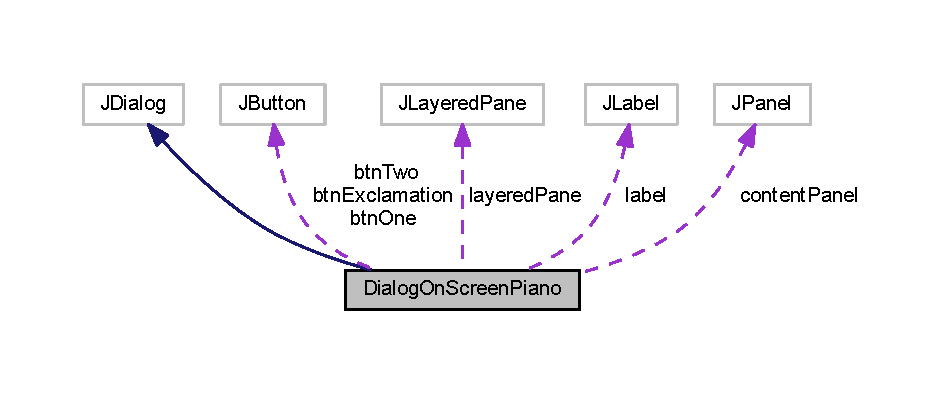
\includegraphics[width=350pt]{classcom_1_1lclion_1_1midigui_1_1_dialog_on_screen_piano__coll__graph}
\end{center}
\end{figure}
\subsection*{Public Member Functions}
\begin{DoxyCompactItemize}
\item 
\hyperlink{classcom_1_1lclion_1_1midigui_1_1_dialog_on_screen_piano_a7a9746635810e3e1a2fd38e7d5bd5934}{Dialog\+On\+Screen\+Piano} (final J\+Frame parent)
\end{DoxyCompactItemize}
\subsection*{Private Attributes}
\begin{DoxyCompactItemize}
\item 
final J\+Panel \hyperlink{classcom_1_1lclion_1_1midigui_1_1_dialog_on_screen_piano_ac383c7b38c74b9e1cc245a00de4fbb5e}{content\+Panel} = new J\+Panel()
\item 
J\+Layered\+Pane \hyperlink{classcom_1_1lclion_1_1midigui_1_1_dialog_on_screen_piano_a90de2803c72845b70771d7326d038f45}{layered\+Pane}
\item 
J\+Label \hyperlink{classcom_1_1lclion_1_1midigui_1_1_dialog_on_screen_piano_ac12cbe37671cd5915541509460b6c16d}{label}
\item 
J\+Button \hyperlink{classcom_1_1lclion_1_1midigui_1_1_dialog_on_screen_piano_aef09a9eab948aa3e07e2b0b7b654efbc}{btn\+One}
\item 
J\+Button \hyperlink{classcom_1_1lclion_1_1midigui_1_1_dialog_on_screen_piano_a88b48836413c071b723ad4a68a51d568}{btn\+Two}
\item 
J\+Button \hyperlink{classcom_1_1lclion_1_1midigui_1_1_dialog_on_screen_piano_a15b11a7d832a97cc78153b959a8607f0}{btn\+Exclamation}
\end{DoxyCompactItemize}


\subsection{Detailed Description}
Displays a preview of a 61-\/keyed piano, indicating the current note played from the main window. 

\begin{DoxyAuthor}{Author}
L\+C Lion 
\end{DoxyAuthor}


\subsection{Constructor \& Destructor Documentation}
\hypertarget{classcom_1_1lclion_1_1midigui_1_1_dialog_on_screen_piano_a7a9746635810e3e1a2fd38e7d5bd5934}{\index{com\+::lclion\+::midigui\+::\+Dialog\+On\+Screen\+Piano@{com\+::lclion\+::midigui\+::\+Dialog\+On\+Screen\+Piano}!Dialog\+On\+Screen\+Piano@{Dialog\+On\+Screen\+Piano}}
\index{Dialog\+On\+Screen\+Piano@{Dialog\+On\+Screen\+Piano}!com\+::lclion\+::midigui\+::\+Dialog\+On\+Screen\+Piano@{com\+::lclion\+::midigui\+::\+Dialog\+On\+Screen\+Piano}}
\subsubsection[{Dialog\+On\+Screen\+Piano}]{\setlength{\rightskip}{0pt plus 5cm}{\bf Dialog\+On\+Screen\+Piano} (
\begin{DoxyParamCaption}
\item[{final J\+Frame}]{parent}
\end{DoxyParamCaption}
)}}\label{classcom_1_1lclion_1_1midigui_1_1_dialog_on_screen_piano_a7a9746635810e3e1a2fd38e7d5bd5934}
Create the dialog. 

\subsection{Member Data Documentation}
\hypertarget{classcom_1_1lclion_1_1midigui_1_1_dialog_on_screen_piano_a15b11a7d832a97cc78153b959a8607f0}{\index{com\+::lclion\+::midigui\+::\+Dialog\+On\+Screen\+Piano@{com\+::lclion\+::midigui\+::\+Dialog\+On\+Screen\+Piano}!btn\+Exclamation@{btn\+Exclamation}}
\index{btn\+Exclamation@{btn\+Exclamation}!com\+::lclion\+::midigui\+::\+Dialog\+On\+Screen\+Piano@{com\+::lclion\+::midigui\+::\+Dialog\+On\+Screen\+Piano}}
\subsubsection[{btn\+Exclamation}]{\setlength{\rightskip}{0pt plus 5cm}J\+Button btn\+Exclamation\hspace{0.3cm}{\ttfamily [private]}}}\label{classcom_1_1lclion_1_1midigui_1_1_dialog_on_screen_piano_a15b11a7d832a97cc78153b959a8607f0}
\hypertarget{classcom_1_1lclion_1_1midigui_1_1_dialog_on_screen_piano_aef09a9eab948aa3e07e2b0b7b654efbc}{\index{com\+::lclion\+::midigui\+::\+Dialog\+On\+Screen\+Piano@{com\+::lclion\+::midigui\+::\+Dialog\+On\+Screen\+Piano}!btn\+One@{btn\+One}}
\index{btn\+One@{btn\+One}!com\+::lclion\+::midigui\+::\+Dialog\+On\+Screen\+Piano@{com\+::lclion\+::midigui\+::\+Dialog\+On\+Screen\+Piano}}
\subsubsection[{btn\+One}]{\setlength{\rightskip}{0pt plus 5cm}J\+Button btn\+One\hspace{0.3cm}{\ttfamily [private]}}}\label{classcom_1_1lclion_1_1midigui_1_1_dialog_on_screen_piano_aef09a9eab948aa3e07e2b0b7b654efbc}
\hypertarget{classcom_1_1lclion_1_1midigui_1_1_dialog_on_screen_piano_a88b48836413c071b723ad4a68a51d568}{\index{com\+::lclion\+::midigui\+::\+Dialog\+On\+Screen\+Piano@{com\+::lclion\+::midigui\+::\+Dialog\+On\+Screen\+Piano}!btn\+Two@{btn\+Two}}
\index{btn\+Two@{btn\+Two}!com\+::lclion\+::midigui\+::\+Dialog\+On\+Screen\+Piano@{com\+::lclion\+::midigui\+::\+Dialog\+On\+Screen\+Piano}}
\subsubsection[{btn\+Two}]{\setlength{\rightskip}{0pt plus 5cm}J\+Button btn\+Two\hspace{0.3cm}{\ttfamily [private]}}}\label{classcom_1_1lclion_1_1midigui_1_1_dialog_on_screen_piano_a88b48836413c071b723ad4a68a51d568}
\hypertarget{classcom_1_1lclion_1_1midigui_1_1_dialog_on_screen_piano_ac383c7b38c74b9e1cc245a00de4fbb5e}{\index{com\+::lclion\+::midigui\+::\+Dialog\+On\+Screen\+Piano@{com\+::lclion\+::midigui\+::\+Dialog\+On\+Screen\+Piano}!content\+Panel@{content\+Panel}}
\index{content\+Panel@{content\+Panel}!com\+::lclion\+::midigui\+::\+Dialog\+On\+Screen\+Piano@{com\+::lclion\+::midigui\+::\+Dialog\+On\+Screen\+Piano}}
\subsubsection[{content\+Panel}]{\setlength{\rightskip}{0pt plus 5cm}final J\+Panel content\+Panel = new J\+Panel()\hspace{0.3cm}{\ttfamily [private]}}}\label{classcom_1_1lclion_1_1midigui_1_1_dialog_on_screen_piano_ac383c7b38c74b9e1cc245a00de4fbb5e}
\hypertarget{classcom_1_1lclion_1_1midigui_1_1_dialog_on_screen_piano_ac12cbe37671cd5915541509460b6c16d}{\index{com\+::lclion\+::midigui\+::\+Dialog\+On\+Screen\+Piano@{com\+::lclion\+::midigui\+::\+Dialog\+On\+Screen\+Piano}!label@{label}}
\index{label@{label}!com\+::lclion\+::midigui\+::\+Dialog\+On\+Screen\+Piano@{com\+::lclion\+::midigui\+::\+Dialog\+On\+Screen\+Piano}}
\subsubsection[{label}]{\setlength{\rightskip}{0pt plus 5cm}J\+Label label\hspace{0.3cm}{\ttfamily [private]}}}\label{classcom_1_1lclion_1_1midigui_1_1_dialog_on_screen_piano_ac12cbe37671cd5915541509460b6c16d}
\hypertarget{classcom_1_1lclion_1_1midigui_1_1_dialog_on_screen_piano_a90de2803c72845b70771d7326d038f45}{\index{com\+::lclion\+::midigui\+::\+Dialog\+On\+Screen\+Piano@{com\+::lclion\+::midigui\+::\+Dialog\+On\+Screen\+Piano}!layered\+Pane@{layered\+Pane}}
\index{layered\+Pane@{layered\+Pane}!com\+::lclion\+::midigui\+::\+Dialog\+On\+Screen\+Piano@{com\+::lclion\+::midigui\+::\+Dialog\+On\+Screen\+Piano}}
\subsubsection[{layered\+Pane}]{\setlength{\rightskip}{0pt plus 5cm}J\+Layered\+Pane layered\+Pane\hspace{0.3cm}{\ttfamily [private]}}}\label{classcom_1_1lclion_1_1midigui_1_1_dialog_on_screen_piano_a90de2803c72845b70771d7326d038f45}


The documentation for this class was generated from the following file\+:\begin{DoxyCompactItemize}
\item 
src/com/lclion/midigui/\hyperlink{_dialog_on_screen_piano_8java}{Dialog\+On\+Screen\+Piano.\+java}\end{DoxyCompactItemize}

\hypertarget{classcom_1_1lclion_1_1midigui_1_1_dialog_preferences}{\section{Dialog\+Preferences Class Reference}
\label{classcom_1_1lclion_1_1midigui_1_1_dialog_preferences}\index{Dialog\+Preferences@{Dialog\+Preferences}}
}


The main preference window where users can configure how M\+I\+D\+I files get imported.  




Collaboration diagram for Dialog\+Preferences\+:\nopagebreak
\begin{figure}[H]
\begin{center}
\leavevmode
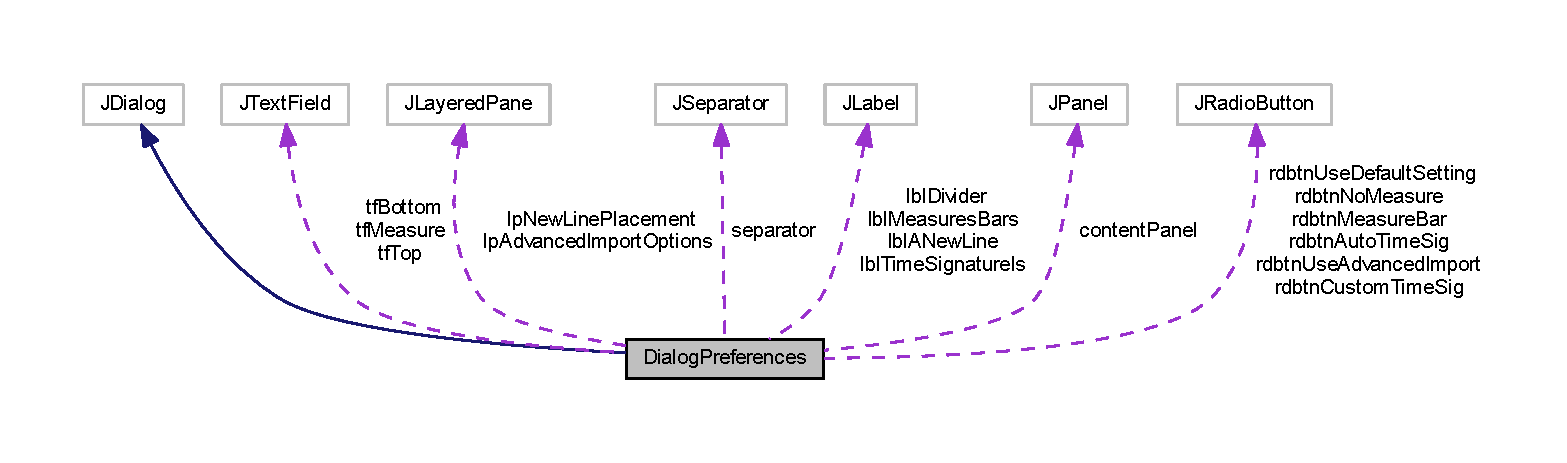
\includegraphics[width=350pt]{classcom_1_1lclion_1_1midigui_1_1_dialog_preferences__coll__graph}
\end{center}
\end{figure}
\subsection*{Public Member Functions}
\begin{DoxyCompactItemize}
\item 
\hyperlink{classcom_1_1lclion_1_1midigui_1_1_dialog_preferences_a3a976528242fb285edfa4844685b2682}{Dialog\+Preferences} (J\+Frame parent)
\item 
boolean \hyperlink{classcom_1_1lclion_1_1midigui_1_1_dialog_preferences_a7550ebb9d4b246937d72d6967e5c1c81}{is\+Custom\+Measure} ()
\item 
int \hyperlink{classcom_1_1lclion_1_1midigui_1_1_dialog_preferences_aecf15bd6d5f5cb5cc99fc780b0f992d9}{get\+Measures} ()
\item 
boolean \hyperlink{classcom_1_1lclion_1_1midigui_1_1_dialog_preferences_a9db6e6d7e71ab42a67aa837f223ba8e1}{is\+Advanced\+Track\+Import} ()
\end{DoxyCompactItemize}
\subsection*{Private Member Functions}
\begin{DoxyCompactItemize}
\item 
void \hyperlink{classcom_1_1lclion_1_1midigui_1_1_dialog_preferences_a67110efd36dc5fb48cd3086a11e39247}{toggle\+Enable\+Time\+Sig} (boolean value)
\item 
void \hyperlink{classcom_1_1lclion_1_1midigui_1_1_dialog_preferences_ab06a00ad2b6aba181568158e22a6490d}{toggle\+Enable\+New\+Line\+Placement} (boolean value)
\end{DoxyCompactItemize}
\subsection*{Private Attributes}
\begin{DoxyCompactItemize}
\item 
final J\+Panel \hyperlink{classcom_1_1lclion_1_1midigui_1_1_dialog_preferences_ac383c7b38c74b9e1cc245a00de4fbb5e}{content\+Panel} = new J\+Panel()
\item 
J\+Radio\+Button \hyperlink{classcom_1_1lclion_1_1midigui_1_1_dialog_preferences_aa403bc56221bd1af763dbf31f90a8902}{rdbtn\+Auto\+Time\+Sig}
\item 
J\+Radio\+Button \hyperlink{classcom_1_1lclion_1_1midigui_1_1_dialog_preferences_ad09e056f314ee875a2c70236299d5633}{rdbtn\+Custom\+Time\+Sig}
\item 
J\+Text\+Field \hyperlink{classcom_1_1lclion_1_1midigui_1_1_dialog_preferences_a1df6442c69813ef29777fef773a4c0f9}{tf\+Top}
\item 
J\+Text\+Field \hyperlink{classcom_1_1lclion_1_1midigui_1_1_dialog_preferences_ad2edc1b54d80700468be7da4535d3fc3}{tf\+Bottom}
\item 
J\+Label \hyperlink{classcom_1_1lclion_1_1midigui_1_1_dialog_preferences_a992b76652c560915d4f052a8718a72dd}{lbl\+Time\+Signature\+Is}
\item 
J\+Layered\+Pane \hyperlink{classcom_1_1lclion_1_1midigui_1_1_dialog_preferences_af502e5d406164d232cafc3abdee20dbd}{lp\+New\+Line\+Placement}
\item 
J\+Radio\+Button \hyperlink{classcom_1_1lclion_1_1midigui_1_1_dialog_preferences_a541603f796912a6a5e40a885d18c2b6d}{rdbtn\+Measure\+Bar}
\item 
J\+Radio\+Button \hyperlink{classcom_1_1lclion_1_1midigui_1_1_dialog_preferences_a4a8eba2702fef7e4d27fa65343a9c637}{rdbtn\+No\+Measure}
\item 
J\+Text\+Field \hyperlink{classcom_1_1lclion_1_1midigui_1_1_dialog_preferences_a66ef301f8f1ef71c2843bb6c2669a86c}{tf\+Measure}
\item 
J\+Label \hyperlink{classcom_1_1lclion_1_1midigui_1_1_dialog_preferences_a923dbec9d9737f58a391ded48df38504}{lbl\+A\+New\+Line}
\item 
J\+Layered\+Pane \hyperlink{classcom_1_1lclion_1_1midigui_1_1_dialog_preferences_a03355431be865e450f20710c67681712}{lp\+Advanced\+Import\+Options}
\item 
J\+Radio\+Button \hyperlink{classcom_1_1lclion_1_1midigui_1_1_dialog_preferences_aaae7fc9e14a38f469e6893b83d5f612c}{rdbtn\+Use\+Advanced\+Import}
\item 
J\+Radio\+Button \hyperlink{classcom_1_1lclion_1_1midigui_1_1_dialog_preferences_a0940277a2ce216beea0ccf7a09a00f96}{rdbtn\+Use\+Default\+Setting}
\item 
J\+Label \hyperlink{classcom_1_1lclion_1_1midigui_1_1_dialog_preferences_a2dfc8604454d799fbab2f9f80c8fb163}{lbl\+Measures\+Bars}
\item 
J\+Label \hyperlink{classcom_1_1lclion_1_1midigui_1_1_dialog_preferences_a4be52faa93d3abb805ffecdc6048bb14}{lbl\+Divider}
\item 
J\+Separator \hyperlink{classcom_1_1lclion_1_1midigui_1_1_dialog_preferences_a450f10fc093a1e45620382f9303a8416}{separator}
\end{DoxyCompactItemize}


\subsection{Detailed Description}
The main preference window where users can configure how M\+I\+D\+I files get imported. 

\begin{DoxyAuthor}{Author}
L\+C Lion 
\end{DoxyAuthor}


\subsection{Constructor \& Destructor Documentation}
\hypertarget{classcom_1_1lclion_1_1midigui_1_1_dialog_preferences_a3a976528242fb285edfa4844685b2682}{\index{com\+::lclion\+::midigui\+::\+Dialog\+Preferences@{com\+::lclion\+::midigui\+::\+Dialog\+Preferences}!Dialog\+Preferences@{Dialog\+Preferences}}
\index{Dialog\+Preferences@{Dialog\+Preferences}!com\+::lclion\+::midigui\+::\+Dialog\+Preferences@{com\+::lclion\+::midigui\+::\+Dialog\+Preferences}}
\subsubsection[{Dialog\+Preferences}]{\setlength{\rightskip}{0pt plus 5cm}{\bf Dialog\+Preferences} (
\begin{DoxyParamCaption}
\item[{J\+Frame}]{parent}
\end{DoxyParamCaption}
)}}\label{classcom_1_1lclion_1_1midigui_1_1_dialog_preferences_a3a976528242fb285edfa4844685b2682}
Create the dialog. 

Here is the call graph for this function\+:\nopagebreak
\begin{figure}[H]
\begin{center}
\leavevmode
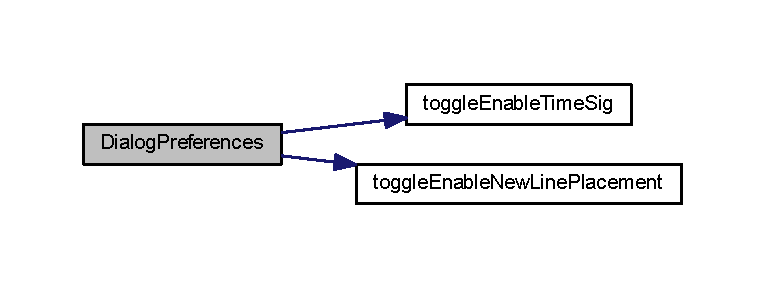
\includegraphics[width=350pt]{classcom_1_1lclion_1_1midigui_1_1_dialog_preferences_a3a976528242fb285edfa4844685b2682_cgraph}
\end{center}
\end{figure}




\subsection{Member Function Documentation}
\hypertarget{classcom_1_1lclion_1_1midigui_1_1_dialog_preferences_aecf15bd6d5f5cb5cc99fc780b0f992d9}{\index{com\+::lclion\+::midigui\+::\+Dialog\+Preferences@{com\+::lclion\+::midigui\+::\+Dialog\+Preferences}!get\+Measures@{get\+Measures}}
\index{get\+Measures@{get\+Measures}!com\+::lclion\+::midigui\+::\+Dialog\+Preferences@{com\+::lclion\+::midigui\+::\+Dialog\+Preferences}}
\subsubsection[{get\+Measures}]{\setlength{\rightskip}{0pt plus 5cm}int get\+Measures (
\begin{DoxyParamCaption}
{}
\end{DoxyParamCaption}
)}}\label{classcom_1_1lclion_1_1midigui_1_1_dialog_preferences_aecf15bd6d5f5cb5cc99fc780b0f992d9}
\hypertarget{classcom_1_1lclion_1_1midigui_1_1_dialog_preferences_a9db6e6d7e71ab42a67aa837f223ba8e1}{\index{com\+::lclion\+::midigui\+::\+Dialog\+Preferences@{com\+::lclion\+::midigui\+::\+Dialog\+Preferences}!is\+Advanced\+Track\+Import@{is\+Advanced\+Track\+Import}}
\index{is\+Advanced\+Track\+Import@{is\+Advanced\+Track\+Import}!com\+::lclion\+::midigui\+::\+Dialog\+Preferences@{com\+::lclion\+::midigui\+::\+Dialog\+Preferences}}
\subsubsection[{is\+Advanced\+Track\+Import}]{\setlength{\rightskip}{0pt plus 5cm}boolean is\+Advanced\+Track\+Import (
\begin{DoxyParamCaption}
{}
\end{DoxyParamCaption}
)}}\label{classcom_1_1lclion_1_1midigui_1_1_dialog_preferences_a9db6e6d7e71ab42a67aa837f223ba8e1}
\hypertarget{classcom_1_1lclion_1_1midigui_1_1_dialog_preferences_a7550ebb9d4b246937d72d6967e5c1c81}{\index{com\+::lclion\+::midigui\+::\+Dialog\+Preferences@{com\+::lclion\+::midigui\+::\+Dialog\+Preferences}!is\+Custom\+Measure@{is\+Custom\+Measure}}
\index{is\+Custom\+Measure@{is\+Custom\+Measure}!com\+::lclion\+::midigui\+::\+Dialog\+Preferences@{com\+::lclion\+::midigui\+::\+Dialog\+Preferences}}
\subsubsection[{is\+Custom\+Measure}]{\setlength{\rightskip}{0pt plus 5cm}boolean is\+Custom\+Measure (
\begin{DoxyParamCaption}
{}
\end{DoxyParamCaption}
)}}\label{classcom_1_1lclion_1_1midigui_1_1_dialog_preferences_a7550ebb9d4b246937d72d6967e5c1c81}
\hypertarget{classcom_1_1lclion_1_1midigui_1_1_dialog_preferences_ab06a00ad2b6aba181568158e22a6490d}{\index{com\+::lclion\+::midigui\+::\+Dialog\+Preferences@{com\+::lclion\+::midigui\+::\+Dialog\+Preferences}!toggle\+Enable\+New\+Line\+Placement@{toggle\+Enable\+New\+Line\+Placement}}
\index{toggle\+Enable\+New\+Line\+Placement@{toggle\+Enable\+New\+Line\+Placement}!com\+::lclion\+::midigui\+::\+Dialog\+Preferences@{com\+::lclion\+::midigui\+::\+Dialog\+Preferences}}
\subsubsection[{toggle\+Enable\+New\+Line\+Placement}]{\setlength{\rightskip}{0pt plus 5cm}void toggle\+Enable\+New\+Line\+Placement (
\begin{DoxyParamCaption}
\item[{boolean}]{value}
\end{DoxyParamCaption}
)\hspace{0.3cm}{\ttfamily [private]}}}\label{classcom_1_1lclion_1_1midigui_1_1_dialog_preferences_ab06a00ad2b6aba181568158e22a6490d}
\hypertarget{classcom_1_1lclion_1_1midigui_1_1_dialog_preferences_a67110efd36dc5fb48cd3086a11e39247}{\index{com\+::lclion\+::midigui\+::\+Dialog\+Preferences@{com\+::lclion\+::midigui\+::\+Dialog\+Preferences}!toggle\+Enable\+Time\+Sig@{toggle\+Enable\+Time\+Sig}}
\index{toggle\+Enable\+Time\+Sig@{toggle\+Enable\+Time\+Sig}!com\+::lclion\+::midigui\+::\+Dialog\+Preferences@{com\+::lclion\+::midigui\+::\+Dialog\+Preferences}}
\subsubsection[{toggle\+Enable\+Time\+Sig}]{\setlength{\rightskip}{0pt plus 5cm}void toggle\+Enable\+Time\+Sig (
\begin{DoxyParamCaption}
\item[{boolean}]{value}
\end{DoxyParamCaption}
)\hspace{0.3cm}{\ttfamily [private]}}}\label{classcom_1_1lclion_1_1midigui_1_1_dialog_preferences_a67110efd36dc5fb48cd3086a11e39247}


\subsection{Member Data Documentation}
\hypertarget{classcom_1_1lclion_1_1midigui_1_1_dialog_preferences_ac383c7b38c74b9e1cc245a00de4fbb5e}{\index{com\+::lclion\+::midigui\+::\+Dialog\+Preferences@{com\+::lclion\+::midigui\+::\+Dialog\+Preferences}!content\+Panel@{content\+Panel}}
\index{content\+Panel@{content\+Panel}!com\+::lclion\+::midigui\+::\+Dialog\+Preferences@{com\+::lclion\+::midigui\+::\+Dialog\+Preferences}}
\subsubsection[{content\+Panel}]{\setlength{\rightskip}{0pt plus 5cm}final J\+Panel content\+Panel = new J\+Panel()\hspace{0.3cm}{\ttfamily [private]}}}\label{classcom_1_1lclion_1_1midigui_1_1_dialog_preferences_ac383c7b38c74b9e1cc245a00de4fbb5e}
\hypertarget{classcom_1_1lclion_1_1midigui_1_1_dialog_preferences_a923dbec9d9737f58a391ded48df38504}{\index{com\+::lclion\+::midigui\+::\+Dialog\+Preferences@{com\+::lclion\+::midigui\+::\+Dialog\+Preferences}!lbl\+A\+New\+Line@{lbl\+A\+New\+Line}}
\index{lbl\+A\+New\+Line@{lbl\+A\+New\+Line}!com\+::lclion\+::midigui\+::\+Dialog\+Preferences@{com\+::lclion\+::midigui\+::\+Dialog\+Preferences}}
\subsubsection[{lbl\+A\+New\+Line}]{\setlength{\rightskip}{0pt plus 5cm}J\+Label lbl\+A\+New\+Line\hspace{0.3cm}{\ttfamily [private]}}}\label{classcom_1_1lclion_1_1midigui_1_1_dialog_preferences_a923dbec9d9737f58a391ded48df38504}
\hypertarget{classcom_1_1lclion_1_1midigui_1_1_dialog_preferences_a4be52faa93d3abb805ffecdc6048bb14}{\index{com\+::lclion\+::midigui\+::\+Dialog\+Preferences@{com\+::lclion\+::midigui\+::\+Dialog\+Preferences}!lbl\+Divider@{lbl\+Divider}}
\index{lbl\+Divider@{lbl\+Divider}!com\+::lclion\+::midigui\+::\+Dialog\+Preferences@{com\+::lclion\+::midigui\+::\+Dialog\+Preferences}}
\subsubsection[{lbl\+Divider}]{\setlength{\rightskip}{0pt plus 5cm}J\+Label lbl\+Divider\hspace{0.3cm}{\ttfamily [private]}}}\label{classcom_1_1lclion_1_1midigui_1_1_dialog_preferences_a4be52faa93d3abb805ffecdc6048bb14}
\hypertarget{classcom_1_1lclion_1_1midigui_1_1_dialog_preferences_a2dfc8604454d799fbab2f9f80c8fb163}{\index{com\+::lclion\+::midigui\+::\+Dialog\+Preferences@{com\+::lclion\+::midigui\+::\+Dialog\+Preferences}!lbl\+Measures\+Bars@{lbl\+Measures\+Bars}}
\index{lbl\+Measures\+Bars@{lbl\+Measures\+Bars}!com\+::lclion\+::midigui\+::\+Dialog\+Preferences@{com\+::lclion\+::midigui\+::\+Dialog\+Preferences}}
\subsubsection[{lbl\+Measures\+Bars}]{\setlength{\rightskip}{0pt plus 5cm}J\+Label lbl\+Measures\+Bars\hspace{0.3cm}{\ttfamily [private]}}}\label{classcom_1_1lclion_1_1midigui_1_1_dialog_preferences_a2dfc8604454d799fbab2f9f80c8fb163}
\hypertarget{classcom_1_1lclion_1_1midigui_1_1_dialog_preferences_a992b76652c560915d4f052a8718a72dd}{\index{com\+::lclion\+::midigui\+::\+Dialog\+Preferences@{com\+::lclion\+::midigui\+::\+Dialog\+Preferences}!lbl\+Time\+Signature\+Is@{lbl\+Time\+Signature\+Is}}
\index{lbl\+Time\+Signature\+Is@{lbl\+Time\+Signature\+Is}!com\+::lclion\+::midigui\+::\+Dialog\+Preferences@{com\+::lclion\+::midigui\+::\+Dialog\+Preferences}}
\subsubsection[{lbl\+Time\+Signature\+Is}]{\setlength{\rightskip}{0pt plus 5cm}J\+Label lbl\+Time\+Signature\+Is\hspace{0.3cm}{\ttfamily [private]}}}\label{classcom_1_1lclion_1_1midigui_1_1_dialog_preferences_a992b76652c560915d4f052a8718a72dd}
\hypertarget{classcom_1_1lclion_1_1midigui_1_1_dialog_preferences_a03355431be865e450f20710c67681712}{\index{com\+::lclion\+::midigui\+::\+Dialog\+Preferences@{com\+::lclion\+::midigui\+::\+Dialog\+Preferences}!lp\+Advanced\+Import\+Options@{lp\+Advanced\+Import\+Options}}
\index{lp\+Advanced\+Import\+Options@{lp\+Advanced\+Import\+Options}!com\+::lclion\+::midigui\+::\+Dialog\+Preferences@{com\+::lclion\+::midigui\+::\+Dialog\+Preferences}}
\subsubsection[{lp\+Advanced\+Import\+Options}]{\setlength{\rightskip}{0pt plus 5cm}J\+Layered\+Pane lp\+Advanced\+Import\+Options\hspace{0.3cm}{\ttfamily [private]}}}\label{classcom_1_1lclion_1_1midigui_1_1_dialog_preferences_a03355431be865e450f20710c67681712}
\hypertarget{classcom_1_1lclion_1_1midigui_1_1_dialog_preferences_af502e5d406164d232cafc3abdee20dbd}{\index{com\+::lclion\+::midigui\+::\+Dialog\+Preferences@{com\+::lclion\+::midigui\+::\+Dialog\+Preferences}!lp\+New\+Line\+Placement@{lp\+New\+Line\+Placement}}
\index{lp\+New\+Line\+Placement@{lp\+New\+Line\+Placement}!com\+::lclion\+::midigui\+::\+Dialog\+Preferences@{com\+::lclion\+::midigui\+::\+Dialog\+Preferences}}
\subsubsection[{lp\+New\+Line\+Placement}]{\setlength{\rightskip}{0pt plus 5cm}J\+Layered\+Pane lp\+New\+Line\+Placement\hspace{0.3cm}{\ttfamily [private]}}}\label{classcom_1_1lclion_1_1midigui_1_1_dialog_preferences_af502e5d406164d232cafc3abdee20dbd}
\hypertarget{classcom_1_1lclion_1_1midigui_1_1_dialog_preferences_aa403bc56221bd1af763dbf31f90a8902}{\index{com\+::lclion\+::midigui\+::\+Dialog\+Preferences@{com\+::lclion\+::midigui\+::\+Dialog\+Preferences}!rdbtn\+Auto\+Time\+Sig@{rdbtn\+Auto\+Time\+Sig}}
\index{rdbtn\+Auto\+Time\+Sig@{rdbtn\+Auto\+Time\+Sig}!com\+::lclion\+::midigui\+::\+Dialog\+Preferences@{com\+::lclion\+::midigui\+::\+Dialog\+Preferences}}
\subsubsection[{rdbtn\+Auto\+Time\+Sig}]{\setlength{\rightskip}{0pt plus 5cm}J\+Radio\+Button rdbtn\+Auto\+Time\+Sig\hspace{0.3cm}{\ttfamily [private]}}}\label{classcom_1_1lclion_1_1midigui_1_1_dialog_preferences_aa403bc56221bd1af763dbf31f90a8902}
\hypertarget{classcom_1_1lclion_1_1midigui_1_1_dialog_preferences_ad09e056f314ee875a2c70236299d5633}{\index{com\+::lclion\+::midigui\+::\+Dialog\+Preferences@{com\+::lclion\+::midigui\+::\+Dialog\+Preferences}!rdbtn\+Custom\+Time\+Sig@{rdbtn\+Custom\+Time\+Sig}}
\index{rdbtn\+Custom\+Time\+Sig@{rdbtn\+Custom\+Time\+Sig}!com\+::lclion\+::midigui\+::\+Dialog\+Preferences@{com\+::lclion\+::midigui\+::\+Dialog\+Preferences}}
\subsubsection[{rdbtn\+Custom\+Time\+Sig}]{\setlength{\rightskip}{0pt plus 5cm}J\+Radio\+Button rdbtn\+Custom\+Time\+Sig\hspace{0.3cm}{\ttfamily [private]}}}\label{classcom_1_1lclion_1_1midigui_1_1_dialog_preferences_ad09e056f314ee875a2c70236299d5633}
\hypertarget{classcom_1_1lclion_1_1midigui_1_1_dialog_preferences_a541603f796912a6a5e40a885d18c2b6d}{\index{com\+::lclion\+::midigui\+::\+Dialog\+Preferences@{com\+::lclion\+::midigui\+::\+Dialog\+Preferences}!rdbtn\+Measure\+Bar@{rdbtn\+Measure\+Bar}}
\index{rdbtn\+Measure\+Bar@{rdbtn\+Measure\+Bar}!com\+::lclion\+::midigui\+::\+Dialog\+Preferences@{com\+::lclion\+::midigui\+::\+Dialog\+Preferences}}
\subsubsection[{rdbtn\+Measure\+Bar}]{\setlength{\rightskip}{0pt plus 5cm}J\+Radio\+Button rdbtn\+Measure\+Bar\hspace{0.3cm}{\ttfamily [private]}}}\label{classcom_1_1lclion_1_1midigui_1_1_dialog_preferences_a541603f796912a6a5e40a885d18c2b6d}
\hypertarget{classcom_1_1lclion_1_1midigui_1_1_dialog_preferences_a4a8eba2702fef7e4d27fa65343a9c637}{\index{com\+::lclion\+::midigui\+::\+Dialog\+Preferences@{com\+::lclion\+::midigui\+::\+Dialog\+Preferences}!rdbtn\+No\+Measure@{rdbtn\+No\+Measure}}
\index{rdbtn\+No\+Measure@{rdbtn\+No\+Measure}!com\+::lclion\+::midigui\+::\+Dialog\+Preferences@{com\+::lclion\+::midigui\+::\+Dialog\+Preferences}}
\subsubsection[{rdbtn\+No\+Measure}]{\setlength{\rightskip}{0pt plus 5cm}J\+Radio\+Button rdbtn\+No\+Measure\hspace{0.3cm}{\ttfamily [private]}}}\label{classcom_1_1lclion_1_1midigui_1_1_dialog_preferences_a4a8eba2702fef7e4d27fa65343a9c637}
\hypertarget{classcom_1_1lclion_1_1midigui_1_1_dialog_preferences_aaae7fc9e14a38f469e6893b83d5f612c}{\index{com\+::lclion\+::midigui\+::\+Dialog\+Preferences@{com\+::lclion\+::midigui\+::\+Dialog\+Preferences}!rdbtn\+Use\+Advanced\+Import@{rdbtn\+Use\+Advanced\+Import}}
\index{rdbtn\+Use\+Advanced\+Import@{rdbtn\+Use\+Advanced\+Import}!com\+::lclion\+::midigui\+::\+Dialog\+Preferences@{com\+::lclion\+::midigui\+::\+Dialog\+Preferences}}
\subsubsection[{rdbtn\+Use\+Advanced\+Import}]{\setlength{\rightskip}{0pt plus 5cm}J\+Radio\+Button rdbtn\+Use\+Advanced\+Import\hspace{0.3cm}{\ttfamily [private]}}}\label{classcom_1_1lclion_1_1midigui_1_1_dialog_preferences_aaae7fc9e14a38f469e6893b83d5f612c}
\hypertarget{classcom_1_1lclion_1_1midigui_1_1_dialog_preferences_a0940277a2ce216beea0ccf7a09a00f96}{\index{com\+::lclion\+::midigui\+::\+Dialog\+Preferences@{com\+::lclion\+::midigui\+::\+Dialog\+Preferences}!rdbtn\+Use\+Default\+Setting@{rdbtn\+Use\+Default\+Setting}}
\index{rdbtn\+Use\+Default\+Setting@{rdbtn\+Use\+Default\+Setting}!com\+::lclion\+::midigui\+::\+Dialog\+Preferences@{com\+::lclion\+::midigui\+::\+Dialog\+Preferences}}
\subsubsection[{rdbtn\+Use\+Default\+Setting}]{\setlength{\rightskip}{0pt plus 5cm}J\+Radio\+Button rdbtn\+Use\+Default\+Setting\hspace{0.3cm}{\ttfamily [private]}}}\label{classcom_1_1lclion_1_1midigui_1_1_dialog_preferences_a0940277a2ce216beea0ccf7a09a00f96}
\hypertarget{classcom_1_1lclion_1_1midigui_1_1_dialog_preferences_a450f10fc093a1e45620382f9303a8416}{\index{com\+::lclion\+::midigui\+::\+Dialog\+Preferences@{com\+::lclion\+::midigui\+::\+Dialog\+Preferences}!separator@{separator}}
\index{separator@{separator}!com\+::lclion\+::midigui\+::\+Dialog\+Preferences@{com\+::lclion\+::midigui\+::\+Dialog\+Preferences}}
\subsubsection[{separator}]{\setlength{\rightskip}{0pt plus 5cm}J\+Separator separator\hspace{0.3cm}{\ttfamily [private]}}}\label{classcom_1_1lclion_1_1midigui_1_1_dialog_preferences_a450f10fc093a1e45620382f9303a8416}
\hypertarget{classcom_1_1lclion_1_1midigui_1_1_dialog_preferences_ad2edc1b54d80700468be7da4535d3fc3}{\index{com\+::lclion\+::midigui\+::\+Dialog\+Preferences@{com\+::lclion\+::midigui\+::\+Dialog\+Preferences}!tf\+Bottom@{tf\+Bottom}}
\index{tf\+Bottom@{tf\+Bottom}!com\+::lclion\+::midigui\+::\+Dialog\+Preferences@{com\+::lclion\+::midigui\+::\+Dialog\+Preferences}}
\subsubsection[{tf\+Bottom}]{\setlength{\rightskip}{0pt plus 5cm}J\+Text\+Field tf\+Bottom\hspace{0.3cm}{\ttfamily [private]}}}\label{classcom_1_1lclion_1_1midigui_1_1_dialog_preferences_ad2edc1b54d80700468be7da4535d3fc3}
\hypertarget{classcom_1_1lclion_1_1midigui_1_1_dialog_preferences_a66ef301f8f1ef71c2843bb6c2669a86c}{\index{com\+::lclion\+::midigui\+::\+Dialog\+Preferences@{com\+::lclion\+::midigui\+::\+Dialog\+Preferences}!tf\+Measure@{tf\+Measure}}
\index{tf\+Measure@{tf\+Measure}!com\+::lclion\+::midigui\+::\+Dialog\+Preferences@{com\+::lclion\+::midigui\+::\+Dialog\+Preferences}}
\subsubsection[{tf\+Measure}]{\setlength{\rightskip}{0pt plus 5cm}J\+Text\+Field tf\+Measure\hspace{0.3cm}{\ttfamily [private]}}}\label{classcom_1_1lclion_1_1midigui_1_1_dialog_preferences_a66ef301f8f1ef71c2843bb6c2669a86c}
\hypertarget{classcom_1_1lclion_1_1midigui_1_1_dialog_preferences_a1df6442c69813ef29777fef773a4c0f9}{\index{com\+::lclion\+::midigui\+::\+Dialog\+Preferences@{com\+::lclion\+::midigui\+::\+Dialog\+Preferences}!tf\+Top@{tf\+Top}}
\index{tf\+Top@{tf\+Top}!com\+::lclion\+::midigui\+::\+Dialog\+Preferences@{com\+::lclion\+::midigui\+::\+Dialog\+Preferences}}
\subsubsection[{tf\+Top}]{\setlength{\rightskip}{0pt plus 5cm}J\+Text\+Field tf\+Top\hspace{0.3cm}{\ttfamily [private]}}}\label{classcom_1_1lclion_1_1midigui_1_1_dialog_preferences_a1df6442c69813ef29777fef773a4c0f9}


The documentation for this class was generated from the following file\+:\begin{DoxyCompactItemize}
\item 
src/com/lclion/midigui/\hyperlink{_dialog_preferences_8java}{Dialog\+Preferences.\+java}\end{DoxyCompactItemize}

\hypertarget{classcom_1_1lclion_1_1midigui_1_1_dialog_track_import}{\section{Dialog\+Track\+Import Class Reference}
\label{classcom_1_1lclion_1_1midigui_1_1_dialog_track_import}\index{Dialog\+Track\+Import@{Dialog\+Track\+Import}}
}


Dialog which displays advanced track importing options. Displayed when importing M\+I\+D\+I files.  




Collaboration diagram for Dialog\+Track\+Import\+:\nopagebreak
\begin{figure}[H]
\begin{center}
\leavevmode
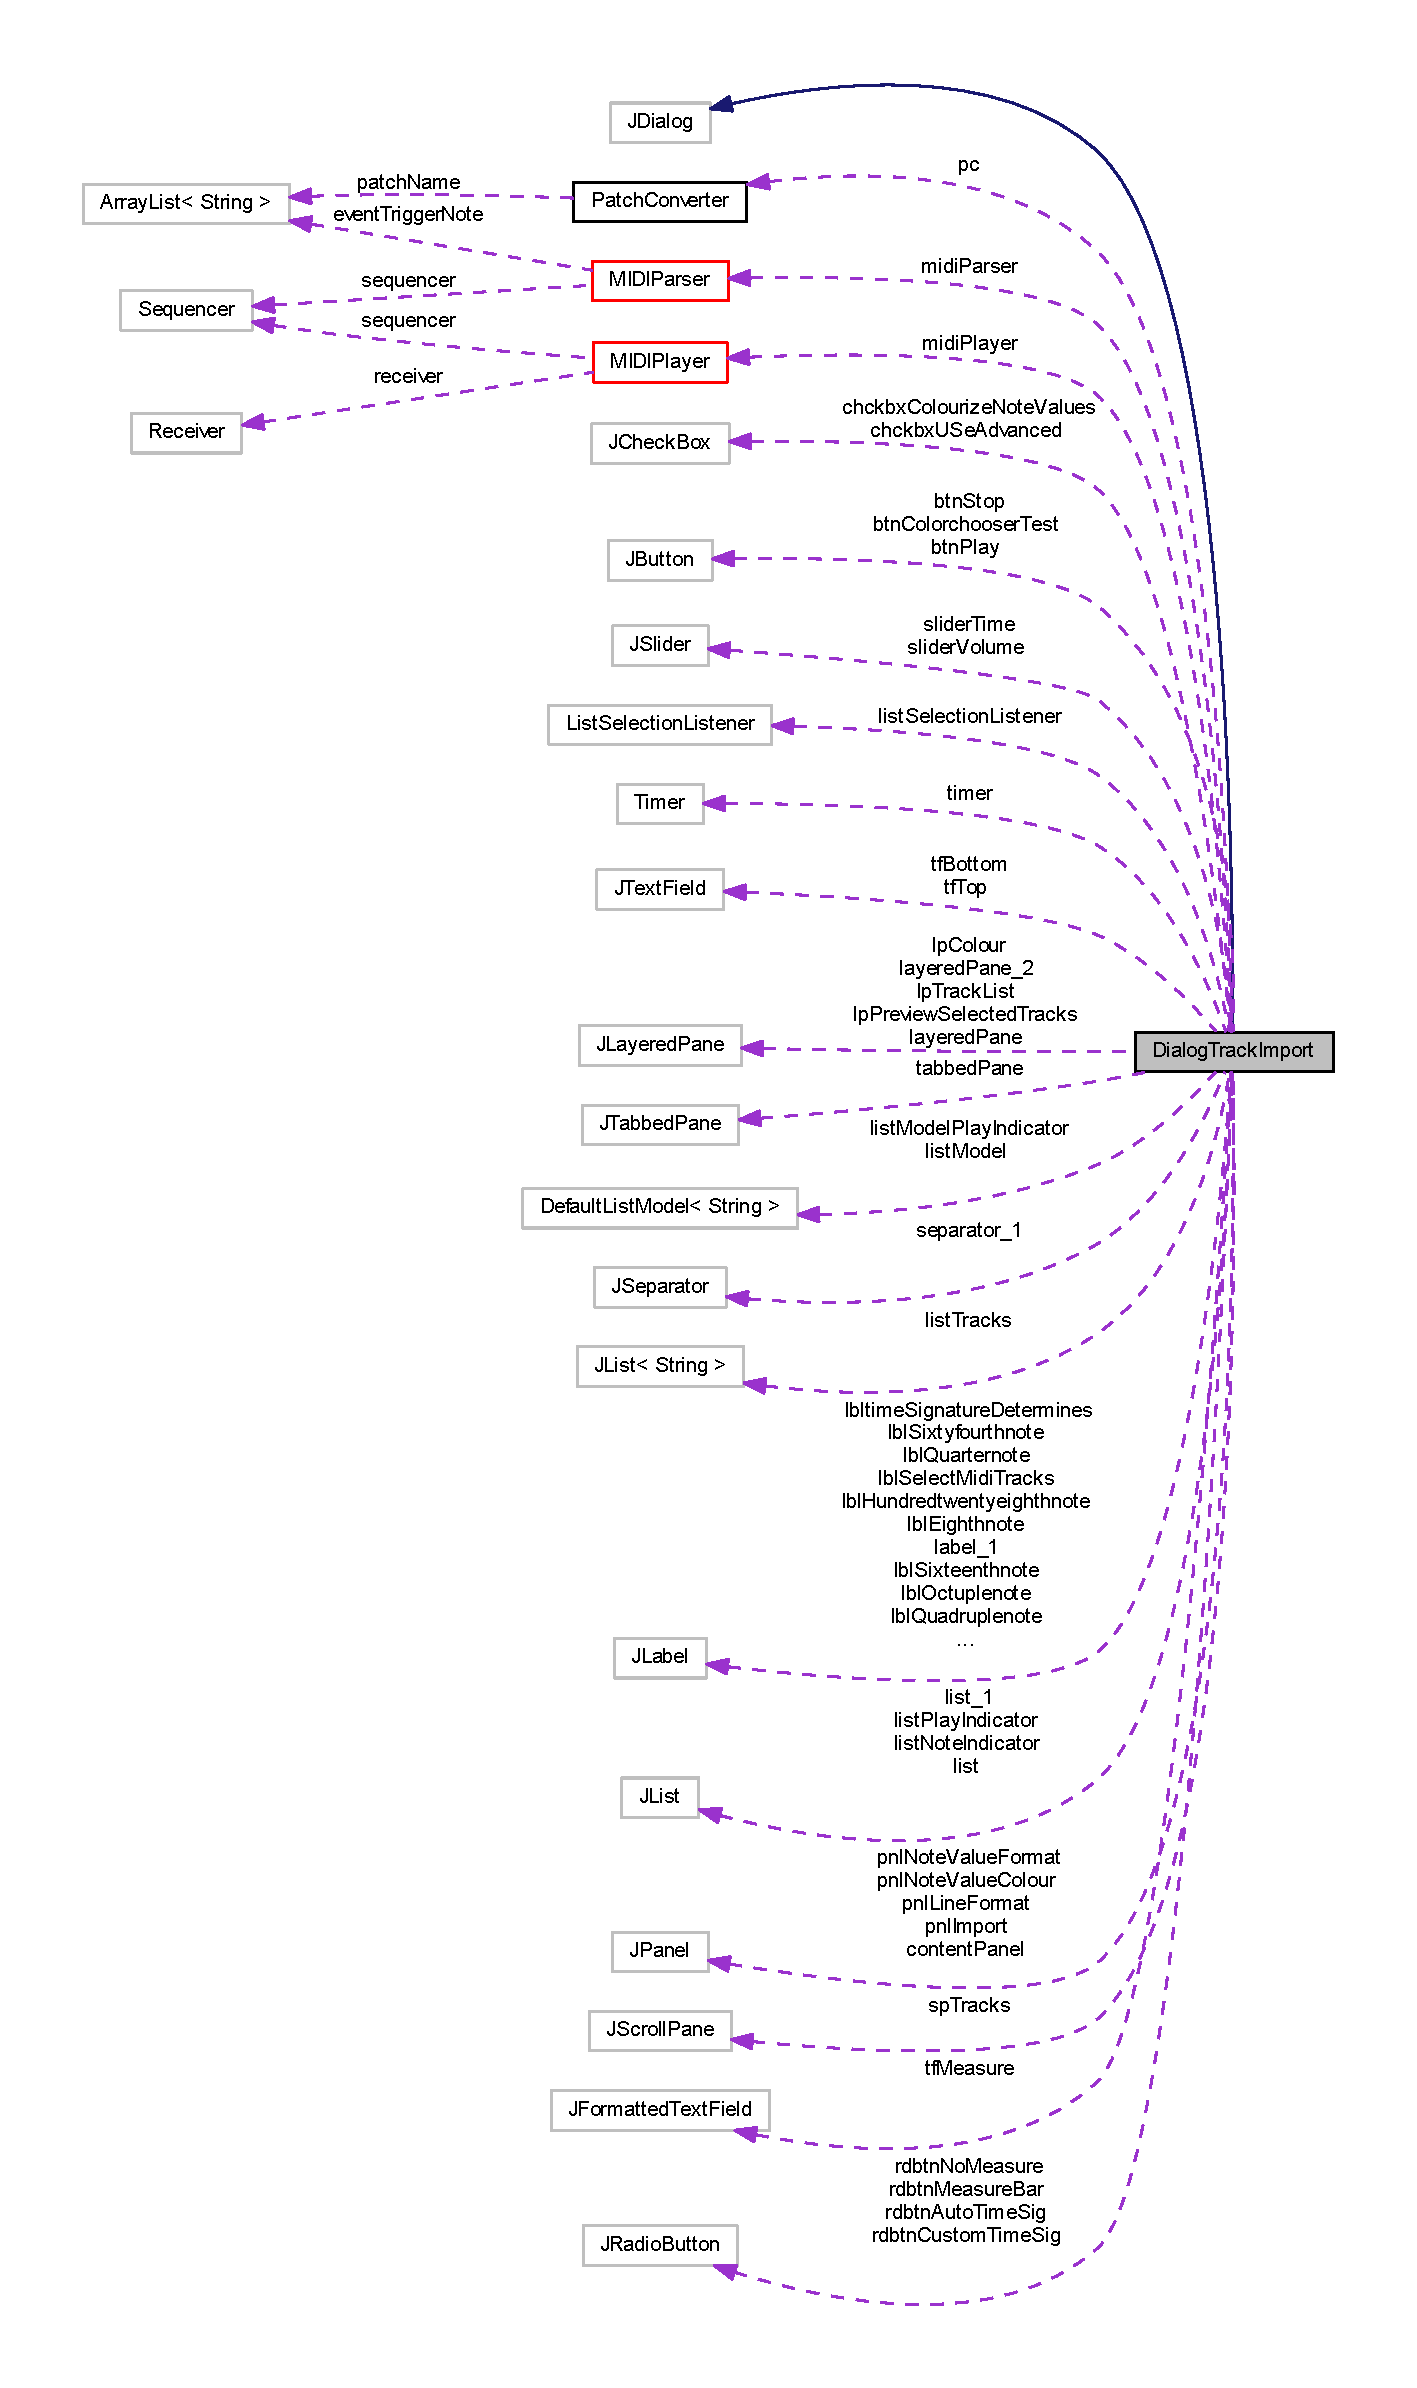
\includegraphics[height=550pt]{classcom_1_1lclion_1_1midigui_1_1_dialog_track_import__coll__graph}
\end{center}
\end{figure}
\subsection*{Public Member Functions}
\begin{DoxyCompactItemize}
\item 
\hyperlink{classcom_1_1lclion_1_1midigui_1_1_dialog_track_import_a2ec034a8f00a81096e52e15c9a4af6a0}{Dialog\+Track\+Import} (J\+Frame parent, File file)
\item 
int \hyperlink{classcom_1_1lclion_1_1midigui_1_1_dialog_track_import_a06989205c167600faad7f71160a05adf}{get\+Selected\+Button} ()
\item 
int \hyperlink{classcom_1_1lclion_1_1midigui_1_1_dialog_track_import_aecf15bd6d5f5cb5cc99fc780b0f992d9}{get\+Measures} ()
\item 
int\mbox{[}$\,$\mbox{]} \hyperlink{classcom_1_1lclion_1_1midigui_1_1_dialog_track_import_a73bbdb2ddcd6001e36559b5c2f65201b}{get\+Selected\+Tracks} ()
\item 
boolean \hyperlink{classcom_1_1lclion_1_1midigui_1_1_dialog_track_import_a7550ebb9d4b246937d72d6967e5c1c81}{is\+Custom\+Measure} ()
\item 
boolean \hyperlink{classcom_1_1lclion_1_1midigui_1_1_dialog_track_import_a31f82d1e457f59ee2e2b76781cf77998}{is\+Colourise} ()
\end{DoxyCompactItemize}
\subsection*{Static Public Attributes}
\begin{DoxyCompactItemize}
\item 
static final int \hyperlink{classcom_1_1lclion_1_1midigui_1_1_dialog_track_import_a0d5e8af086fbdf1f855bbc114cd0a41b}{O\+K\+\_\+\+B\+U\+T\+T\+O\+N} = 1
\item 
static final int \hyperlink{classcom_1_1lclion_1_1midigui_1_1_dialog_track_import_a2728e079b37f5a8285d238ac2cc8224f}{C\+A\+N\+C\+E\+L\+\_\+\+B\+U\+T\+T\+O\+N} = 0
\end{DoxyCompactItemize}
\subsection*{Package Attributes}
\begin{DoxyCompactItemize}
\item 
\hyperlink{classcom_1_1lclion_1_1midiplayer_1_1_m_i_d_i_player}{M\+I\+D\+I\+Player} \hyperlink{classcom_1_1lclion_1_1midigui_1_1_dialog_track_import_ab4562caaf138ca21b1013043d3eb158d}{midi\+Player} = null
\item 
Timer \hyperlink{classcom_1_1lclion_1_1midigui_1_1_dialog_track_import_aaf7e0389622e8f7b78393ee10d8e93a4}{timer} = null
\item 
Default\+List\+Model$<$ String $>$ \hyperlink{classcom_1_1lclion_1_1midigui_1_1_dialog_track_import_acfc0ecfa0a6e94d900b31a8212d60c97}{list\+Model} = null
\end{DoxyCompactItemize}
\subsection*{Private Member Functions}
\begin{DoxyCompactItemize}
\item 
void \hyperlink{classcom_1_1lclion_1_1midigui_1_1_dialog_track_import_ab5f5b7d46d664f092c40a045618402b5}{setup\+Preview\+Player} ()
\item 
void \hyperlink{classcom_1_1lclion_1_1midigui_1_1_dialog_track_import_a8d5ad9e40f8a718ad1a74d164c9c89cd}{setup\+Import\+Listing} (Track\mbox{[}$\,$\mbox{]} tracks)
\end{DoxyCompactItemize}
\subsection*{Private Attributes}
\begin{DoxyCompactItemize}
\item 
final J\+Panel \hyperlink{classcom_1_1lclion_1_1midigui_1_1_dialog_track_import_ac383c7b38c74b9e1cc245a00de4fbb5e}{content\+Panel} = new J\+Panel()
\item 
J\+Scroll\+Pane \hyperlink{classcom_1_1lclion_1_1midigui_1_1_dialog_track_import_a844df9120f38157448c7658bc2d8a1a7}{sp\+Tracks}
\item 
J\+List \hyperlink{classcom_1_1lclion_1_1midigui_1_1_dialog_track_import_aa1bcfa7d07c255e455ca5515e0369310}{list} = null
\item 
J\+Layered\+Pane \hyperlink{classcom_1_1lclion_1_1midigui_1_1_dialog_track_import_a04703476bb0bc1cd0fdbe05cf3d46858}{lp\+Preview\+Selected\+Tracks}
\item 
J\+Slider \hyperlink{classcom_1_1lclion_1_1midigui_1_1_dialog_track_import_a8f1c2180a937d6483a4912d602dfe023}{slider\+Time}
\item 
J\+Button \hyperlink{classcom_1_1lclion_1_1midigui_1_1_dialog_track_import_aa1718d1d474c9cc2c8f72edef9c6d767}{btn\+Play}
\item 
J\+Button \hyperlink{classcom_1_1lclion_1_1midigui_1_1_dialog_track_import_a3e498460ccccf41b258ee18a8ea8d988}{btn\+Stop}
\item 
J\+Slider \hyperlink{classcom_1_1lclion_1_1midigui_1_1_dialog_track_import_a71f41e4a3f136fb318fb088bd4695dc2}{slider\+Volume}
\item 
J\+Label \hyperlink{classcom_1_1lclion_1_1midigui_1_1_dialog_track_import_a8501b39c874b5ed02e4c630f78aa5de5}{lbl\+Volume}
\item 
boolean \hyperlink{classcom_1_1lclion_1_1midigui_1_1_dialog_track_import_aec5da3d6a3d10d8707c05f13ff00e7ac}{is\+Playing} = false
\item 
List\+Selection\+Listener \hyperlink{classcom_1_1lclion_1_1midigui_1_1_dialog_track_import_afc740efab3ca321614150cdc795f841d}{list\+Selection\+Listener} = null
\item 
Default\+List\+Model$<$ String $>$ \hyperlink{classcom_1_1lclion_1_1midigui_1_1_dialog_track_import_a633a346cf94f727ba816e3f85788d1f1}{list\+Model\+Play\+Indicator} = new Default\+List\+Model$<$String$>$()
\item 
int \hyperlink{classcom_1_1lclion_1_1midigui_1_1_dialog_track_import_acddc2ec0ef9a995af7cb614afbdd3f46}{selected\+Button}
\item 
J\+List$<$ String $>$ \hyperlink{classcom_1_1lclion_1_1midigui_1_1_dialog_track_import_a37595f2a0234ab4d9a8b01e23e4997be}{list\+Tracks}
\item 
J\+Layered\+Pane \hyperlink{classcom_1_1lclion_1_1midigui_1_1_dialog_track_import_a90de2803c72845b70771d7326d038f45}{layered\+Pane}
\item 
J\+Radio\+Button \hyperlink{classcom_1_1lclion_1_1midigui_1_1_dialog_track_import_a4a8eba2702fef7e4d27fa65343a9c637}{rdbtn\+No\+Measure}
\item 
J\+Radio\+Button \hyperlink{classcom_1_1lclion_1_1midigui_1_1_dialog_track_import_a541603f796912a6a5e40a885d18c2b6d}{rdbtn\+Measure\+Bar}
\item 
J\+Formatted\+Text\+Field \hyperlink{classcom_1_1lclion_1_1midigui_1_1_dialog_track_import_a6cc62464f9541b65d27a3a7a2ccdcc7b}{tf\+Measure}
\item 
J\+Label \hyperlink{classcom_1_1lclion_1_1midigui_1_1_dialog_track_import_ac12cbe37671cd5915541509460b6c16d}{label}
\item 
J\+Label \hyperlink{classcom_1_1lclion_1_1midigui_1_1_dialog_track_import_a8e0e71bac1a2f7dc57eee4c2bdb3b4c8}{label\+\_\+1}
\item 
J\+Separator \hyperlink{classcom_1_1lclion_1_1midigui_1_1_dialog_track_import_aa3830aae8fa2c36c0acbe8dfb03688bb}{separator\+\_\+1}
\item 
J\+Label \hyperlink{classcom_1_1lclion_1_1midigui_1_1_dialog_track_import_a55a5f9a736ca9e5564e99a75475f665e}{lbltime\+Signature\+Determines}
\item 
J\+Radio\+Button \hyperlink{classcom_1_1lclion_1_1midigui_1_1_dialog_track_import_aa403bc56221bd1af763dbf31f90a8902}{rdbtn\+Auto\+Time\+Sig}
\item 
J\+Radio\+Button \hyperlink{classcom_1_1lclion_1_1midigui_1_1_dialog_track_import_ad09e056f314ee875a2c70236299d5633}{rdbtn\+Custom\+Time\+Sig}
\item 
J\+Text\+Field \hyperlink{classcom_1_1lclion_1_1midigui_1_1_dialog_track_import_a1df6442c69813ef29777fef773a4c0f9}{tf\+Top}
\item 
J\+Text\+Field \hyperlink{classcom_1_1lclion_1_1midigui_1_1_dialog_track_import_ad2edc1b54d80700468be7da4535d3fc3}{tf\+Bottom}
\item 
J\+Label \hyperlink{classcom_1_1lclion_1_1midigui_1_1_dialog_track_import_a7f6cf2680790da7a8524b4fd64c9f04d}{label\+\_\+3}
\item 
J\+Layered\+Pane \hyperlink{classcom_1_1lclion_1_1midigui_1_1_dialog_track_import_a355d53023163856ae9e762dffc32d9e0}{lp\+Track\+List}
\item 
\hyperlink{classcom_1_1lclion_1_1midiparser_1_1_m_i_d_i_parser}{M\+I\+D\+I\+Parser} \hyperlink{classcom_1_1lclion_1_1midigui_1_1_dialog_track_import_aba18751017d64d85cea94d280c8e9dc0}{midi\+Parser} = null
\item 
J\+Tabbed\+Pane \hyperlink{classcom_1_1lclion_1_1midigui_1_1_dialog_track_import_aabdef38c0485e13cc93dc138342e4245}{tabbed\+Pane}
\item 
J\+Panel \hyperlink{classcom_1_1lclion_1_1midigui_1_1_dialog_track_import_a063461ce812abd701b93ebc7b9febb5f}{pnl\+Import}
\item 
J\+Panel \hyperlink{classcom_1_1lclion_1_1midigui_1_1_dialog_track_import_ad869cf75b335e3801223a73a4c0f6662}{pnl\+Line\+Format}
\item 
J\+Panel \hyperlink{classcom_1_1lclion_1_1midigui_1_1_dialog_track_import_a65201fce5439e97384f6b927a7550be2}{pnl\+Note\+Value\+Format}
\item 
J\+List \hyperlink{classcom_1_1lclion_1_1midigui_1_1_dialog_track_import_a8448bcb31eca04209e4985f870f95315}{list\+Note\+Indicator}
\item 
J\+Panel \hyperlink{classcom_1_1lclion_1_1midigui_1_1_dialog_track_import_a0c95d840f4e0fcda4909967c37c6d781}{pnl\+Note\+Value\+Colour}
\item 
J\+Check\+Box \hyperlink{classcom_1_1lclion_1_1midigui_1_1_dialog_track_import_a59dc935aec2200b178464745e0a145ee}{chckbx\+Colourize\+Note\+Values}
\item 
J\+Layered\+Pane \hyperlink{classcom_1_1lclion_1_1midigui_1_1_dialog_track_import_a770ef37f70c3f6f0dfb3e212de32d74c}{lp\+Colour}
\item 
J\+Check\+Box \hyperlink{classcom_1_1lclion_1_1midigui_1_1_dialog_track_import_a372664d11a9dd7bcc42dea9bc2c58823}{chckbx\+U\+Se\+Advanced}
\item 
J\+Layered\+Pane \hyperlink{classcom_1_1lclion_1_1midigui_1_1_dialog_track_import_ae3a0497765f00d7c86b33d5b71d6bc53}{layered\+Pane\+\_\+2}
\item 
J\+Label \hyperlink{classcom_1_1lclion_1_1midigui_1_1_dialog_track_import_ab6faff098d93514ed68471244b9dca08}{lbl\+Only\+Selected\+Tracks}
\item 
J\+Label \hyperlink{classcom_1_1lclion_1_1midigui_1_1_dialog_track_import_ad4f278f27ad89812d6ed6e2394ce9cc1}{lbl\+Octuplenote}
\item 
J\+Label \hyperlink{classcom_1_1lclion_1_1midigui_1_1_dialog_track_import_a7816a2e010eec64ffc3174d617cf35df}{lbl\+Quadruplenote}
\item 
J\+Label \hyperlink{classcom_1_1lclion_1_1midigui_1_1_dialog_track_import_ac7d0bd7b65f556b4d22af7330dd76dcc}{lbl\+Wholenote}
\item 
J\+Label \hyperlink{classcom_1_1lclion_1_1midigui_1_1_dialog_track_import_acfcb2859ddf942402ad2cacd6667927d}{lbl\+Halfnote}
\item 
J\+Label \hyperlink{classcom_1_1lclion_1_1midigui_1_1_dialog_track_import_ae5cfb7a856d76c093ed85d9e8d0548bd}{lbl\+Quarternote}
\item 
J\+Label \hyperlink{classcom_1_1lclion_1_1midigui_1_1_dialog_track_import_a12dd2fd5b473e16168d5cc9b53b064a1}{lbl\+Eighthnote}
\item 
J\+Label \hyperlink{classcom_1_1lclion_1_1midigui_1_1_dialog_track_import_a9ea6ef5b9dce4d50407ffceffd2825a5}{lbl\+Sixteenthnote}
\item 
J\+Label \hyperlink{classcom_1_1lclion_1_1midigui_1_1_dialog_track_import_a70c665b64629375a224fe62984806e5e}{lbl\+Thirtysecondnote}
\item 
J\+Label \hyperlink{classcom_1_1lclion_1_1midigui_1_1_dialog_track_import_a56ec877aa439e951f0a2a4f5b3a5a1bb}{lbl\+Sixtyfourthnote}
\item 
J\+Label \hyperlink{classcom_1_1lclion_1_1midigui_1_1_dialog_track_import_a78f15a440795871a9eab7aa4111114e0}{lbl\+Hundredtwentyeighthnote}
\item 
J\+Label \hyperlink{classcom_1_1lclion_1_1midigui_1_1_dialog_track_import_a9cdecbe937d5853a3e6c5cdf1d0db1e5}{lbl\+Twohundredfiftysixthnote}
\item 
J\+Button \hyperlink{classcom_1_1lclion_1_1midigui_1_1_dialog_track_import_acf6001c3f20d4daa3dcec1516a72a276}{btn\+Colorchooser\+Test}
\item 
J\+List \hyperlink{classcom_1_1lclion_1_1midigui_1_1_dialog_track_import_a7271a6017c882f92a2022cc6cc688fb0}{list\+Play\+Indicator}
\item 
J\+List \hyperlink{classcom_1_1lclion_1_1midigui_1_1_dialog_track_import_a8f0df5ab6c1a8287af5ce9ff2fcfd8e3}{list\+\_\+1}
\item 
J\+Label \hyperlink{classcom_1_1lclion_1_1midigui_1_1_dialog_track_import_a3f8471fb3f216ae539154e089ce46ee7}{lbl\+Select\+Midi\+Tracks}
\item 
J\+Label \hyperlink{classcom_1_1lclion_1_1midigui_1_1_dialog_track_import_aad844b17249eb755348b263953102b01}{lbl\+Events}
\end{DoxyCompactItemize}
\subsection*{Static Private Attributes}
\begin{DoxyCompactItemize}
\item 
static final \hyperlink{classcom_1_1lclion_1_1midiparser_1_1_patch_converter}{Patch\+Converter} \hyperlink{classcom_1_1lclion_1_1midigui_1_1_dialog_track_import_a629a55ce1fe3a51976a23411dcf2ca13}{pc} = new \hyperlink{classcom_1_1lclion_1_1midiparser_1_1_patch_converter}{Patch\+Converter}()
\end{DoxyCompactItemize}


\subsection{Detailed Description}
Dialog which displays advanced track importing options. Displayed when importing M\+I\+D\+I files. 

\begin{DoxyAuthor}{Author}
L\+C Lion 
\end{DoxyAuthor}


\subsection{Constructor \& Destructor Documentation}
\hypertarget{classcom_1_1lclion_1_1midigui_1_1_dialog_track_import_a2ec034a8f00a81096e52e15c9a4af6a0}{\index{com\+::lclion\+::midigui\+::\+Dialog\+Track\+Import@{com\+::lclion\+::midigui\+::\+Dialog\+Track\+Import}!Dialog\+Track\+Import@{Dialog\+Track\+Import}}
\index{Dialog\+Track\+Import@{Dialog\+Track\+Import}!com\+::lclion\+::midigui\+::\+Dialog\+Track\+Import@{com\+::lclion\+::midigui\+::\+Dialog\+Track\+Import}}
\subsubsection[{Dialog\+Track\+Import}]{\setlength{\rightskip}{0pt plus 5cm}{\bf Dialog\+Track\+Import} (
\begin{DoxyParamCaption}
\item[{J\+Frame}]{parent, }
\item[{File}]{file}
\end{DoxyParamCaption}
)}}\label{classcom_1_1lclion_1_1midigui_1_1_dialog_track_import_a2ec034a8f00a81096e52e15c9a4af6a0}
Create the dialog. 

Here is the call graph for this function\+:\nopagebreak
\begin{figure}[H]
\begin{center}
\leavevmode
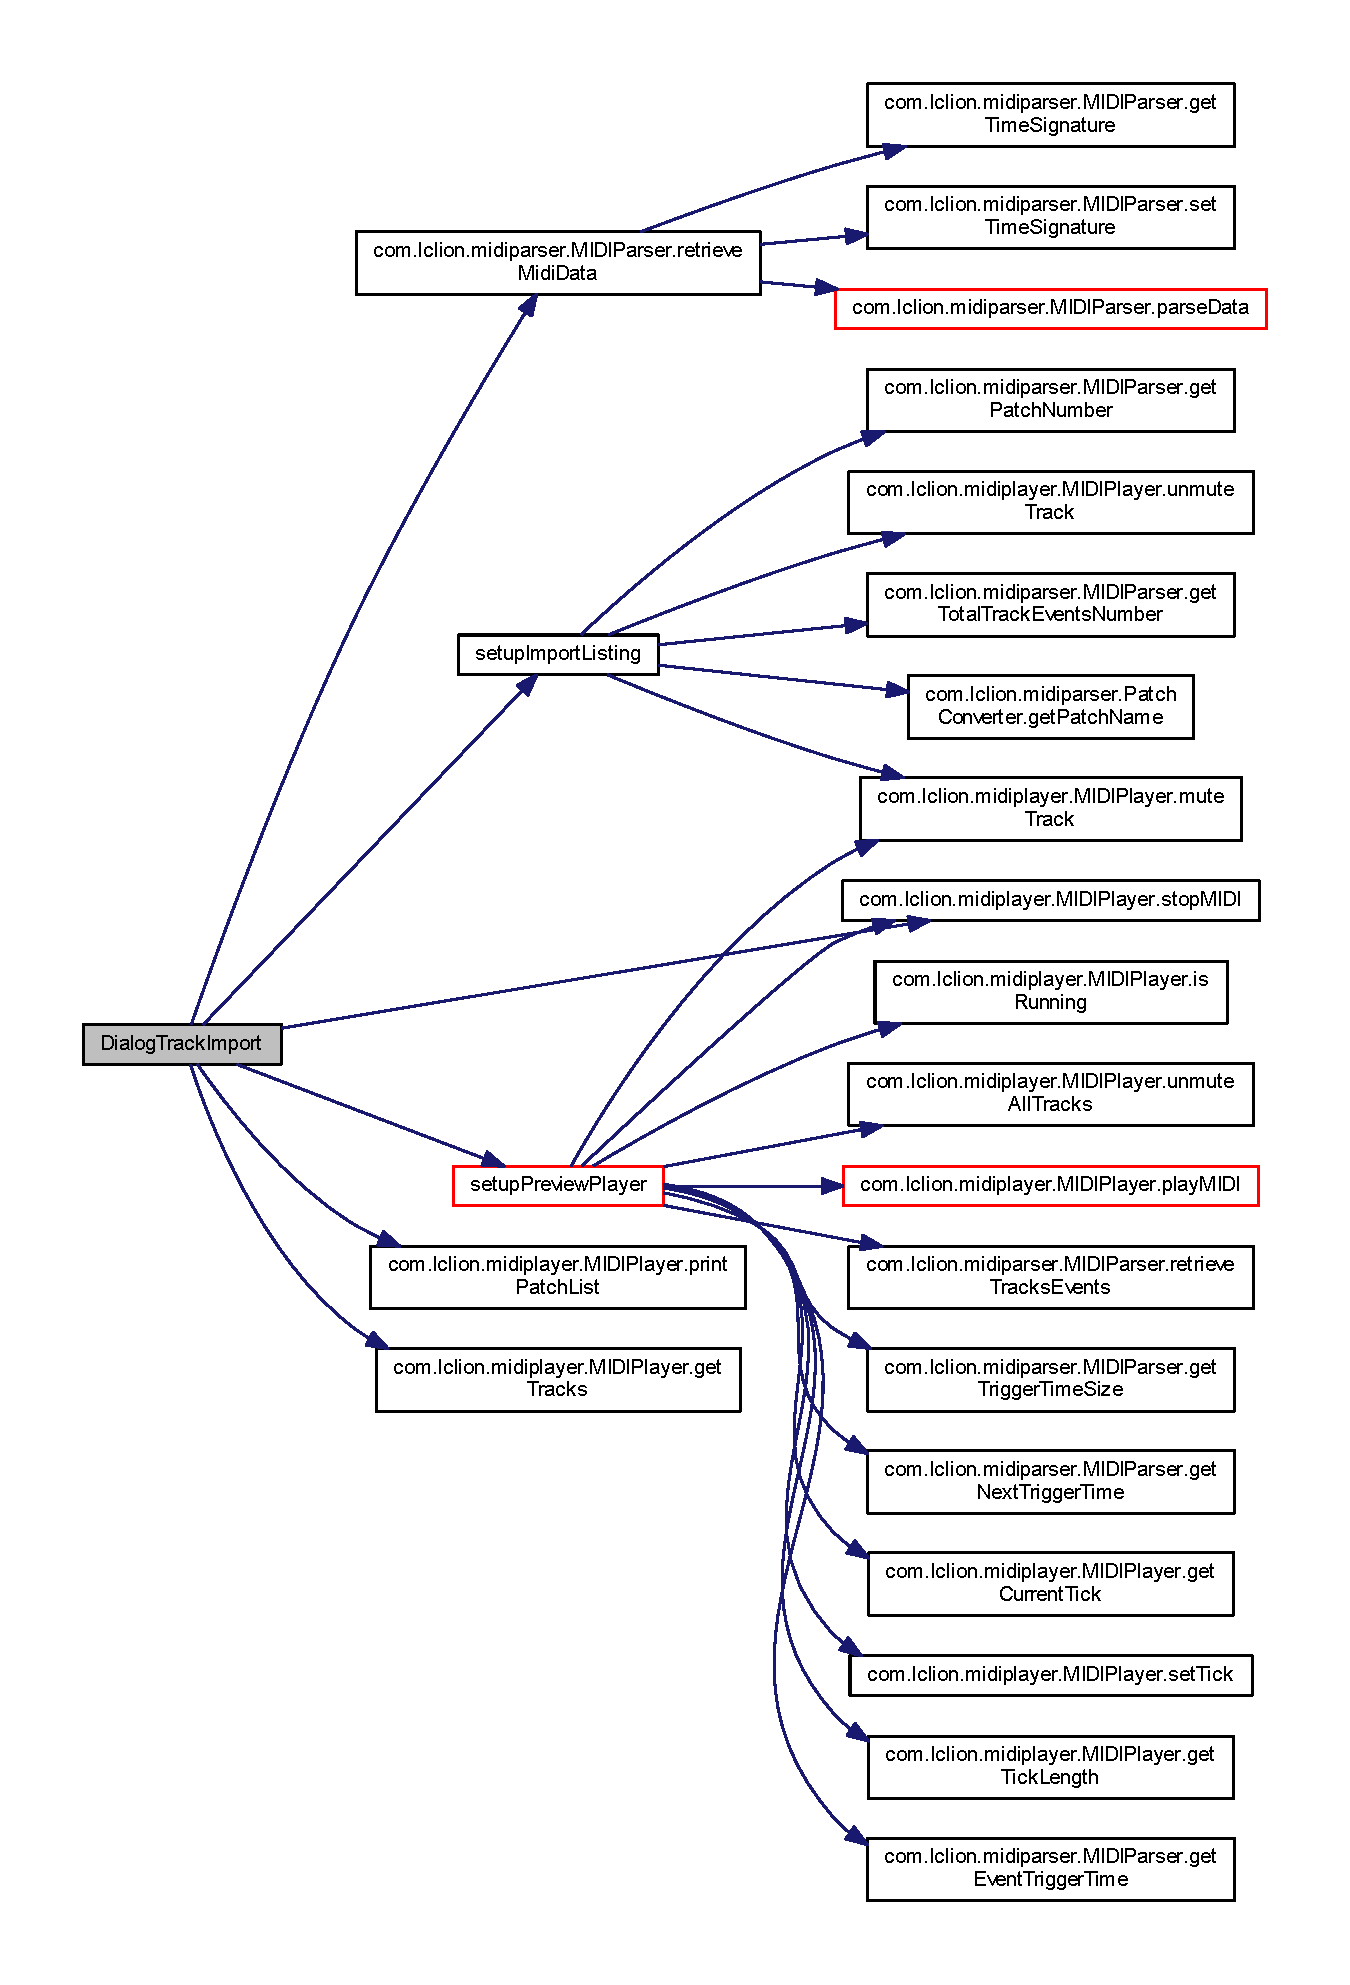
\includegraphics[width=350pt]{classcom_1_1lclion_1_1midigui_1_1_dialog_track_import_a2ec034a8f00a81096e52e15c9a4af6a0_cgraph}
\end{center}
\end{figure}




\subsection{Member Function Documentation}
\hypertarget{classcom_1_1lclion_1_1midigui_1_1_dialog_track_import_aecf15bd6d5f5cb5cc99fc780b0f992d9}{\index{com\+::lclion\+::midigui\+::\+Dialog\+Track\+Import@{com\+::lclion\+::midigui\+::\+Dialog\+Track\+Import}!get\+Measures@{get\+Measures}}
\index{get\+Measures@{get\+Measures}!com\+::lclion\+::midigui\+::\+Dialog\+Track\+Import@{com\+::lclion\+::midigui\+::\+Dialog\+Track\+Import}}
\subsubsection[{get\+Measures}]{\setlength{\rightskip}{0pt plus 5cm}int get\+Measures (
\begin{DoxyParamCaption}
{}
\end{DoxyParamCaption}
)}}\label{classcom_1_1lclion_1_1midigui_1_1_dialog_track_import_aecf15bd6d5f5cb5cc99fc780b0f992d9}
\hypertarget{classcom_1_1lclion_1_1midigui_1_1_dialog_track_import_a06989205c167600faad7f71160a05adf}{\index{com\+::lclion\+::midigui\+::\+Dialog\+Track\+Import@{com\+::lclion\+::midigui\+::\+Dialog\+Track\+Import}!get\+Selected\+Button@{get\+Selected\+Button}}
\index{get\+Selected\+Button@{get\+Selected\+Button}!com\+::lclion\+::midigui\+::\+Dialog\+Track\+Import@{com\+::lclion\+::midigui\+::\+Dialog\+Track\+Import}}
\subsubsection[{get\+Selected\+Button}]{\setlength{\rightskip}{0pt plus 5cm}int get\+Selected\+Button (
\begin{DoxyParamCaption}
{}
\end{DoxyParamCaption}
)}}\label{classcom_1_1lclion_1_1midigui_1_1_dialog_track_import_a06989205c167600faad7f71160a05adf}
\hypertarget{classcom_1_1lclion_1_1midigui_1_1_dialog_track_import_a73bbdb2ddcd6001e36559b5c2f65201b}{\index{com\+::lclion\+::midigui\+::\+Dialog\+Track\+Import@{com\+::lclion\+::midigui\+::\+Dialog\+Track\+Import}!get\+Selected\+Tracks@{get\+Selected\+Tracks}}
\index{get\+Selected\+Tracks@{get\+Selected\+Tracks}!com\+::lclion\+::midigui\+::\+Dialog\+Track\+Import@{com\+::lclion\+::midigui\+::\+Dialog\+Track\+Import}}
\subsubsection[{get\+Selected\+Tracks}]{\setlength{\rightskip}{0pt plus 5cm}int \mbox{[}$\,$\mbox{]} get\+Selected\+Tracks (
\begin{DoxyParamCaption}
{}
\end{DoxyParamCaption}
)}}\label{classcom_1_1lclion_1_1midigui_1_1_dialog_track_import_a73bbdb2ddcd6001e36559b5c2f65201b}
\hypertarget{classcom_1_1lclion_1_1midigui_1_1_dialog_track_import_a31f82d1e457f59ee2e2b76781cf77998}{\index{com\+::lclion\+::midigui\+::\+Dialog\+Track\+Import@{com\+::lclion\+::midigui\+::\+Dialog\+Track\+Import}!is\+Colourise@{is\+Colourise}}
\index{is\+Colourise@{is\+Colourise}!com\+::lclion\+::midigui\+::\+Dialog\+Track\+Import@{com\+::lclion\+::midigui\+::\+Dialog\+Track\+Import}}
\subsubsection[{is\+Colourise}]{\setlength{\rightskip}{0pt plus 5cm}boolean is\+Colourise (
\begin{DoxyParamCaption}
{}
\end{DoxyParamCaption}
)}}\label{classcom_1_1lclion_1_1midigui_1_1_dialog_track_import_a31f82d1e457f59ee2e2b76781cf77998}
\hypertarget{classcom_1_1lclion_1_1midigui_1_1_dialog_track_import_a7550ebb9d4b246937d72d6967e5c1c81}{\index{com\+::lclion\+::midigui\+::\+Dialog\+Track\+Import@{com\+::lclion\+::midigui\+::\+Dialog\+Track\+Import}!is\+Custom\+Measure@{is\+Custom\+Measure}}
\index{is\+Custom\+Measure@{is\+Custom\+Measure}!com\+::lclion\+::midigui\+::\+Dialog\+Track\+Import@{com\+::lclion\+::midigui\+::\+Dialog\+Track\+Import}}
\subsubsection[{is\+Custom\+Measure}]{\setlength{\rightskip}{0pt plus 5cm}boolean is\+Custom\+Measure (
\begin{DoxyParamCaption}
{}
\end{DoxyParamCaption}
)}}\label{classcom_1_1lclion_1_1midigui_1_1_dialog_track_import_a7550ebb9d4b246937d72d6967e5c1c81}
\hypertarget{classcom_1_1lclion_1_1midigui_1_1_dialog_track_import_a8d5ad9e40f8a718ad1a74d164c9c89cd}{\index{com\+::lclion\+::midigui\+::\+Dialog\+Track\+Import@{com\+::lclion\+::midigui\+::\+Dialog\+Track\+Import}!setup\+Import\+Listing@{setup\+Import\+Listing}}
\index{setup\+Import\+Listing@{setup\+Import\+Listing}!com\+::lclion\+::midigui\+::\+Dialog\+Track\+Import@{com\+::lclion\+::midigui\+::\+Dialog\+Track\+Import}}
\subsubsection[{setup\+Import\+Listing}]{\setlength{\rightskip}{0pt plus 5cm}void setup\+Import\+Listing (
\begin{DoxyParamCaption}
\item[{Track\mbox{[}$\,$\mbox{]}}]{tracks}
\end{DoxyParamCaption}
)\hspace{0.3cm}{\ttfamily [private]}}}\label{classcom_1_1lclion_1_1midigui_1_1_dialog_track_import_a8d5ad9e40f8a718ad1a74d164c9c89cd}


Here is the call graph for this function\+:\nopagebreak
\begin{figure}[H]
\begin{center}
\leavevmode
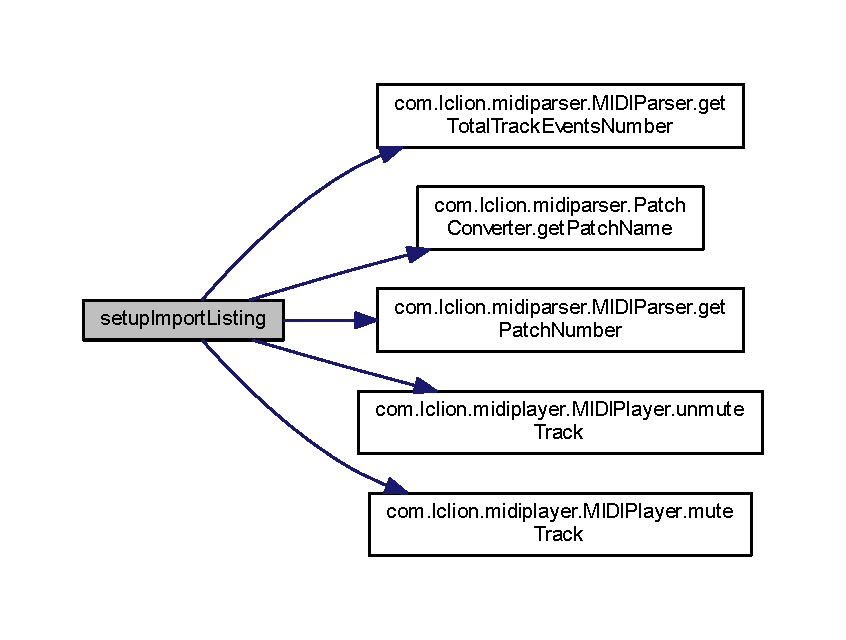
\includegraphics[width=350pt]{classcom_1_1lclion_1_1midigui_1_1_dialog_track_import_a8d5ad9e40f8a718ad1a74d164c9c89cd_cgraph}
\end{center}
\end{figure}


\hypertarget{classcom_1_1lclion_1_1midigui_1_1_dialog_track_import_ab5f5b7d46d664f092c40a045618402b5}{\index{com\+::lclion\+::midigui\+::\+Dialog\+Track\+Import@{com\+::lclion\+::midigui\+::\+Dialog\+Track\+Import}!setup\+Preview\+Player@{setup\+Preview\+Player}}
\index{setup\+Preview\+Player@{setup\+Preview\+Player}!com\+::lclion\+::midigui\+::\+Dialog\+Track\+Import@{com\+::lclion\+::midigui\+::\+Dialog\+Track\+Import}}
\subsubsection[{setup\+Preview\+Player}]{\setlength{\rightskip}{0pt plus 5cm}void setup\+Preview\+Player (
\begin{DoxyParamCaption}
{}
\end{DoxyParamCaption}
)\hspace{0.3cm}{\ttfamily [private]}}}\label{classcom_1_1lclion_1_1midigui_1_1_dialog_track_import_ab5f5b7d46d664f092c40a045618402b5}


Here is the call graph for this function\+:\nopagebreak
\begin{figure}[H]
\begin{center}
\leavevmode
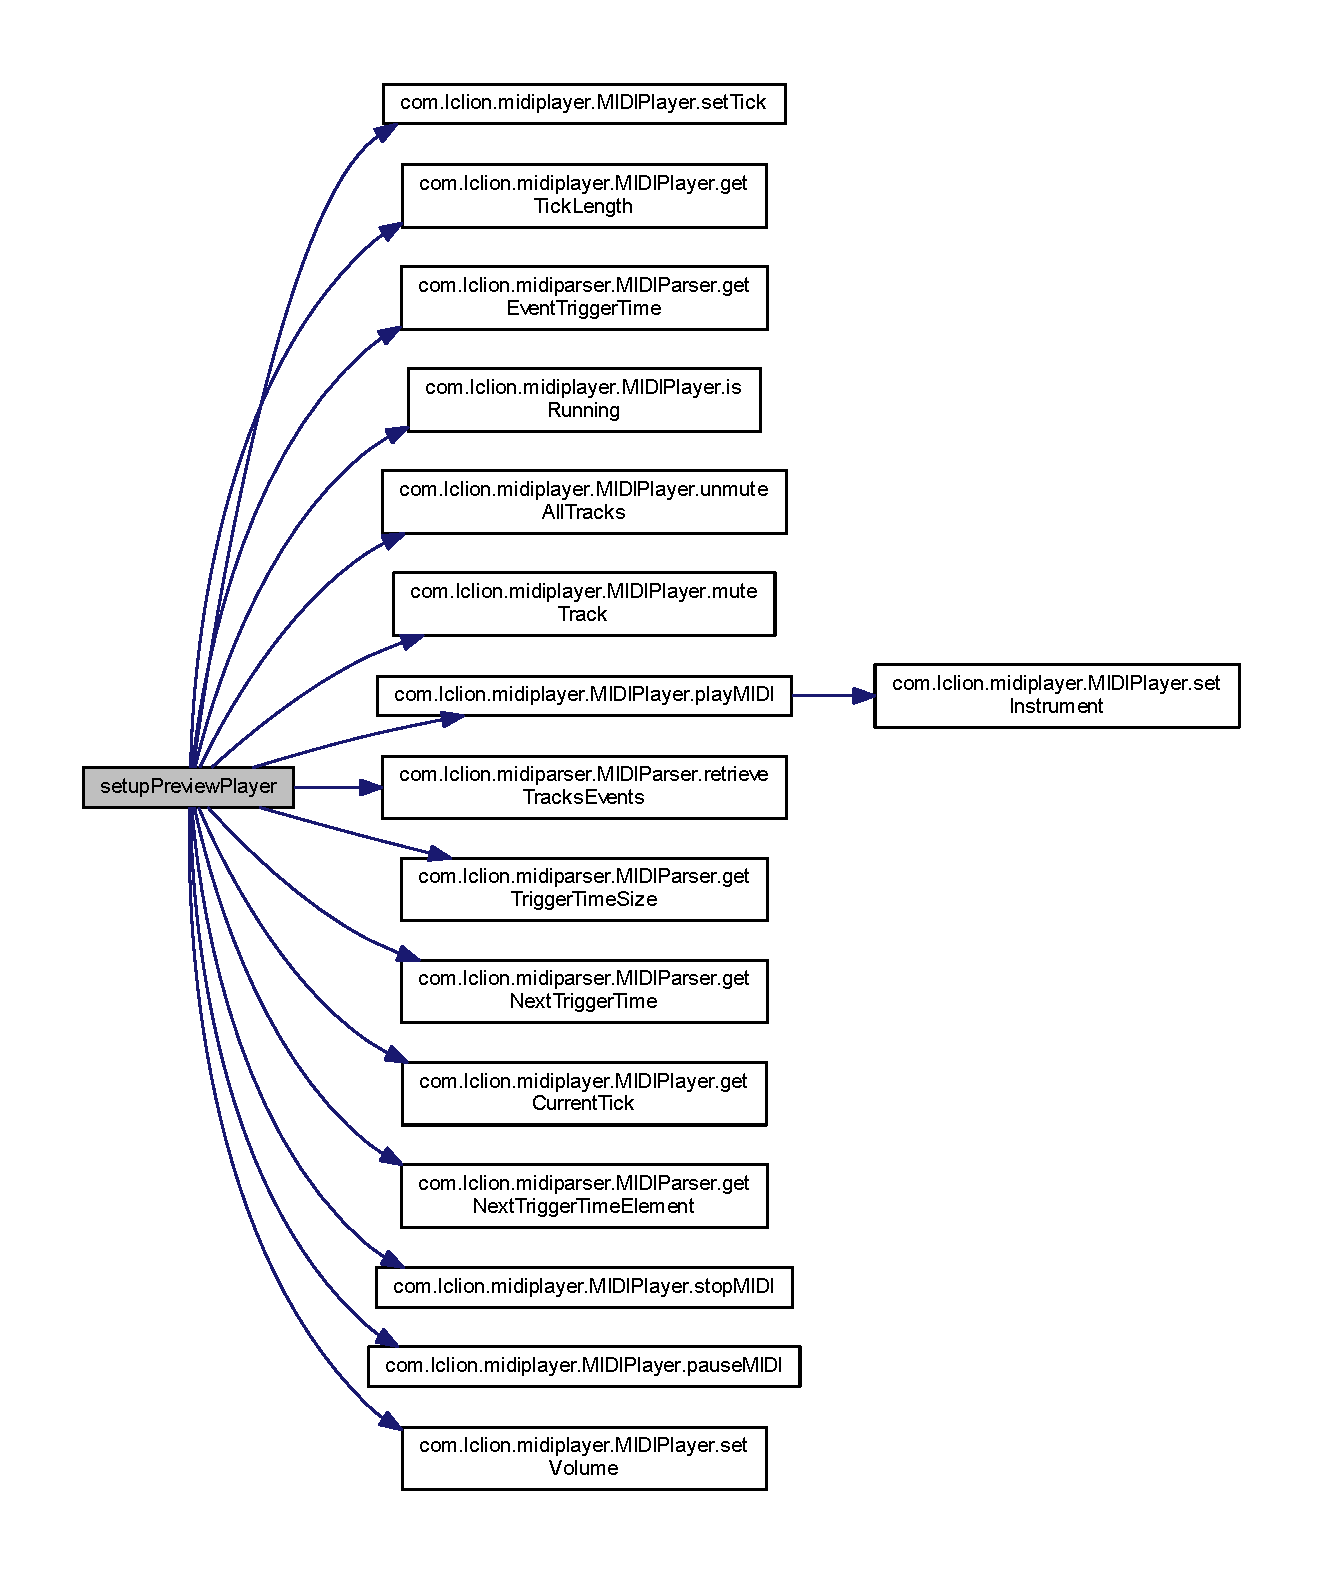
\includegraphics[width=350pt]{classcom_1_1lclion_1_1midigui_1_1_dialog_track_import_ab5f5b7d46d664f092c40a045618402b5_cgraph}
\end{center}
\end{figure}




\subsection{Member Data Documentation}
\hypertarget{classcom_1_1lclion_1_1midigui_1_1_dialog_track_import_acf6001c3f20d4daa3dcec1516a72a276}{\index{com\+::lclion\+::midigui\+::\+Dialog\+Track\+Import@{com\+::lclion\+::midigui\+::\+Dialog\+Track\+Import}!btn\+Colorchooser\+Test@{btn\+Colorchooser\+Test}}
\index{btn\+Colorchooser\+Test@{btn\+Colorchooser\+Test}!com\+::lclion\+::midigui\+::\+Dialog\+Track\+Import@{com\+::lclion\+::midigui\+::\+Dialog\+Track\+Import}}
\subsubsection[{btn\+Colorchooser\+Test}]{\setlength{\rightskip}{0pt plus 5cm}J\+Button btn\+Colorchooser\+Test\hspace{0.3cm}{\ttfamily [private]}}}\label{classcom_1_1lclion_1_1midigui_1_1_dialog_track_import_acf6001c3f20d4daa3dcec1516a72a276}
\hypertarget{classcom_1_1lclion_1_1midigui_1_1_dialog_track_import_aa1718d1d474c9cc2c8f72edef9c6d767}{\index{com\+::lclion\+::midigui\+::\+Dialog\+Track\+Import@{com\+::lclion\+::midigui\+::\+Dialog\+Track\+Import}!btn\+Play@{btn\+Play}}
\index{btn\+Play@{btn\+Play}!com\+::lclion\+::midigui\+::\+Dialog\+Track\+Import@{com\+::lclion\+::midigui\+::\+Dialog\+Track\+Import}}
\subsubsection[{btn\+Play}]{\setlength{\rightskip}{0pt plus 5cm}J\+Button btn\+Play\hspace{0.3cm}{\ttfamily [private]}}}\label{classcom_1_1lclion_1_1midigui_1_1_dialog_track_import_aa1718d1d474c9cc2c8f72edef9c6d767}
\hypertarget{classcom_1_1lclion_1_1midigui_1_1_dialog_track_import_a3e498460ccccf41b258ee18a8ea8d988}{\index{com\+::lclion\+::midigui\+::\+Dialog\+Track\+Import@{com\+::lclion\+::midigui\+::\+Dialog\+Track\+Import}!btn\+Stop@{btn\+Stop}}
\index{btn\+Stop@{btn\+Stop}!com\+::lclion\+::midigui\+::\+Dialog\+Track\+Import@{com\+::lclion\+::midigui\+::\+Dialog\+Track\+Import}}
\subsubsection[{btn\+Stop}]{\setlength{\rightskip}{0pt plus 5cm}J\+Button btn\+Stop\hspace{0.3cm}{\ttfamily [private]}}}\label{classcom_1_1lclion_1_1midigui_1_1_dialog_track_import_a3e498460ccccf41b258ee18a8ea8d988}
\hypertarget{classcom_1_1lclion_1_1midigui_1_1_dialog_track_import_a2728e079b37f5a8285d238ac2cc8224f}{\index{com\+::lclion\+::midigui\+::\+Dialog\+Track\+Import@{com\+::lclion\+::midigui\+::\+Dialog\+Track\+Import}!C\+A\+N\+C\+E\+L\+\_\+\+B\+U\+T\+T\+O\+N@{C\+A\+N\+C\+E\+L\+\_\+\+B\+U\+T\+T\+O\+N}}
\index{C\+A\+N\+C\+E\+L\+\_\+\+B\+U\+T\+T\+O\+N@{C\+A\+N\+C\+E\+L\+\_\+\+B\+U\+T\+T\+O\+N}!com\+::lclion\+::midigui\+::\+Dialog\+Track\+Import@{com\+::lclion\+::midigui\+::\+Dialog\+Track\+Import}}
\subsubsection[{C\+A\+N\+C\+E\+L\+\_\+\+B\+U\+T\+T\+O\+N}]{\setlength{\rightskip}{0pt plus 5cm}final int C\+A\+N\+C\+E\+L\+\_\+\+B\+U\+T\+T\+O\+N = 0\hspace{0.3cm}{\ttfamily [static]}}}\label{classcom_1_1lclion_1_1midigui_1_1_dialog_track_import_a2728e079b37f5a8285d238ac2cc8224f}
\hypertarget{classcom_1_1lclion_1_1midigui_1_1_dialog_track_import_a59dc935aec2200b178464745e0a145ee}{\index{com\+::lclion\+::midigui\+::\+Dialog\+Track\+Import@{com\+::lclion\+::midigui\+::\+Dialog\+Track\+Import}!chckbx\+Colourize\+Note\+Values@{chckbx\+Colourize\+Note\+Values}}
\index{chckbx\+Colourize\+Note\+Values@{chckbx\+Colourize\+Note\+Values}!com\+::lclion\+::midigui\+::\+Dialog\+Track\+Import@{com\+::lclion\+::midigui\+::\+Dialog\+Track\+Import}}
\subsubsection[{chckbx\+Colourize\+Note\+Values}]{\setlength{\rightskip}{0pt plus 5cm}J\+Check\+Box chckbx\+Colourize\+Note\+Values\hspace{0.3cm}{\ttfamily [private]}}}\label{classcom_1_1lclion_1_1midigui_1_1_dialog_track_import_a59dc935aec2200b178464745e0a145ee}
\hypertarget{classcom_1_1lclion_1_1midigui_1_1_dialog_track_import_a372664d11a9dd7bcc42dea9bc2c58823}{\index{com\+::lclion\+::midigui\+::\+Dialog\+Track\+Import@{com\+::lclion\+::midigui\+::\+Dialog\+Track\+Import}!chckbx\+U\+Se\+Advanced@{chckbx\+U\+Se\+Advanced}}
\index{chckbx\+U\+Se\+Advanced@{chckbx\+U\+Se\+Advanced}!com\+::lclion\+::midigui\+::\+Dialog\+Track\+Import@{com\+::lclion\+::midigui\+::\+Dialog\+Track\+Import}}
\subsubsection[{chckbx\+U\+Se\+Advanced}]{\setlength{\rightskip}{0pt plus 5cm}J\+Check\+Box chckbx\+U\+Se\+Advanced\hspace{0.3cm}{\ttfamily [private]}}}\label{classcom_1_1lclion_1_1midigui_1_1_dialog_track_import_a372664d11a9dd7bcc42dea9bc2c58823}
\hypertarget{classcom_1_1lclion_1_1midigui_1_1_dialog_track_import_ac383c7b38c74b9e1cc245a00de4fbb5e}{\index{com\+::lclion\+::midigui\+::\+Dialog\+Track\+Import@{com\+::lclion\+::midigui\+::\+Dialog\+Track\+Import}!content\+Panel@{content\+Panel}}
\index{content\+Panel@{content\+Panel}!com\+::lclion\+::midigui\+::\+Dialog\+Track\+Import@{com\+::lclion\+::midigui\+::\+Dialog\+Track\+Import}}
\subsubsection[{content\+Panel}]{\setlength{\rightskip}{0pt plus 5cm}final J\+Panel content\+Panel = new J\+Panel()\hspace{0.3cm}{\ttfamily [private]}}}\label{classcom_1_1lclion_1_1midigui_1_1_dialog_track_import_ac383c7b38c74b9e1cc245a00de4fbb5e}
\hypertarget{classcom_1_1lclion_1_1midigui_1_1_dialog_track_import_aec5da3d6a3d10d8707c05f13ff00e7ac}{\index{com\+::lclion\+::midigui\+::\+Dialog\+Track\+Import@{com\+::lclion\+::midigui\+::\+Dialog\+Track\+Import}!is\+Playing@{is\+Playing}}
\index{is\+Playing@{is\+Playing}!com\+::lclion\+::midigui\+::\+Dialog\+Track\+Import@{com\+::lclion\+::midigui\+::\+Dialog\+Track\+Import}}
\subsubsection[{is\+Playing}]{\setlength{\rightskip}{0pt plus 5cm}boolean is\+Playing = false\hspace{0.3cm}{\ttfamily [private]}}}\label{classcom_1_1lclion_1_1midigui_1_1_dialog_track_import_aec5da3d6a3d10d8707c05f13ff00e7ac}
\hypertarget{classcom_1_1lclion_1_1midigui_1_1_dialog_track_import_ac12cbe37671cd5915541509460b6c16d}{\index{com\+::lclion\+::midigui\+::\+Dialog\+Track\+Import@{com\+::lclion\+::midigui\+::\+Dialog\+Track\+Import}!label@{label}}
\index{label@{label}!com\+::lclion\+::midigui\+::\+Dialog\+Track\+Import@{com\+::lclion\+::midigui\+::\+Dialog\+Track\+Import}}
\subsubsection[{label}]{\setlength{\rightskip}{0pt plus 5cm}J\+Label label\hspace{0.3cm}{\ttfamily [private]}}}\label{classcom_1_1lclion_1_1midigui_1_1_dialog_track_import_ac12cbe37671cd5915541509460b6c16d}
\hypertarget{classcom_1_1lclion_1_1midigui_1_1_dialog_track_import_a8e0e71bac1a2f7dc57eee4c2bdb3b4c8}{\index{com\+::lclion\+::midigui\+::\+Dialog\+Track\+Import@{com\+::lclion\+::midigui\+::\+Dialog\+Track\+Import}!label\+\_\+1@{label\+\_\+1}}
\index{label\+\_\+1@{label\+\_\+1}!com\+::lclion\+::midigui\+::\+Dialog\+Track\+Import@{com\+::lclion\+::midigui\+::\+Dialog\+Track\+Import}}
\subsubsection[{label\+\_\+1}]{\setlength{\rightskip}{0pt plus 5cm}J\+Label label\+\_\+1\hspace{0.3cm}{\ttfamily [private]}}}\label{classcom_1_1lclion_1_1midigui_1_1_dialog_track_import_a8e0e71bac1a2f7dc57eee4c2bdb3b4c8}
\hypertarget{classcom_1_1lclion_1_1midigui_1_1_dialog_track_import_a7f6cf2680790da7a8524b4fd64c9f04d}{\index{com\+::lclion\+::midigui\+::\+Dialog\+Track\+Import@{com\+::lclion\+::midigui\+::\+Dialog\+Track\+Import}!label\+\_\+3@{label\+\_\+3}}
\index{label\+\_\+3@{label\+\_\+3}!com\+::lclion\+::midigui\+::\+Dialog\+Track\+Import@{com\+::lclion\+::midigui\+::\+Dialog\+Track\+Import}}
\subsubsection[{label\+\_\+3}]{\setlength{\rightskip}{0pt plus 5cm}J\+Label label\+\_\+3\hspace{0.3cm}{\ttfamily [private]}}}\label{classcom_1_1lclion_1_1midigui_1_1_dialog_track_import_a7f6cf2680790da7a8524b4fd64c9f04d}
\hypertarget{classcom_1_1lclion_1_1midigui_1_1_dialog_track_import_a90de2803c72845b70771d7326d038f45}{\index{com\+::lclion\+::midigui\+::\+Dialog\+Track\+Import@{com\+::lclion\+::midigui\+::\+Dialog\+Track\+Import}!layered\+Pane@{layered\+Pane}}
\index{layered\+Pane@{layered\+Pane}!com\+::lclion\+::midigui\+::\+Dialog\+Track\+Import@{com\+::lclion\+::midigui\+::\+Dialog\+Track\+Import}}
\subsubsection[{layered\+Pane}]{\setlength{\rightskip}{0pt plus 5cm}J\+Layered\+Pane layered\+Pane\hspace{0.3cm}{\ttfamily [private]}}}\label{classcom_1_1lclion_1_1midigui_1_1_dialog_track_import_a90de2803c72845b70771d7326d038f45}
\hypertarget{classcom_1_1lclion_1_1midigui_1_1_dialog_track_import_ae3a0497765f00d7c86b33d5b71d6bc53}{\index{com\+::lclion\+::midigui\+::\+Dialog\+Track\+Import@{com\+::lclion\+::midigui\+::\+Dialog\+Track\+Import}!layered\+Pane\+\_\+2@{layered\+Pane\+\_\+2}}
\index{layered\+Pane\+\_\+2@{layered\+Pane\+\_\+2}!com\+::lclion\+::midigui\+::\+Dialog\+Track\+Import@{com\+::lclion\+::midigui\+::\+Dialog\+Track\+Import}}
\subsubsection[{layered\+Pane\+\_\+2}]{\setlength{\rightskip}{0pt plus 5cm}J\+Layered\+Pane layered\+Pane\+\_\+2\hspace{0.3cm}{\ttfamily [private]}}}\label{classcom_1_1lclion_1_1midigui_1_1_dialog_track_import_ae3a0497765f00d7c86b33d5b71d6bc53}
\hypertarget{classcom_1_1lclion_1_1midigui_1_1_dialog_track_import_a12dd2fd5b473e16168d5cc9b53b064a1}{\index{com\+::lclion\+::midigui\+::\+Dialog\+Track\+Import@{com\+::lclion\+::midigui\+::\+Dialog\+Track\+Import}!lbl\+Eighthnote@{lbl\+Eighthnote}}
\index{lbl\+Eighthnote@{lbl\+Eighthnote}!com\+::lclion\+::midigui\+::\+Dialog\+Track\+Import@{com\+::lclion\+::midigui\+::\+Dialog\+Track\+Import}}
\subsubsection[{lbl\+Eighthnote}]{\setlength{\rightskip}{0pt plus 5cm}J\+Label lbl\+Eighthnote\hspace{0.3cm}{\ttfamily [private]}}}\label{classcom_1_1lclion_1_1midigui_1_1_dialog_track_import_a12dd2fd5b473e16168d5cc9b53b064a1}
\hypertarget{classcom_1_1lclion_1_1midigui_1_1_dialog_track_import_aad844b17249eb755348b263953102b01}{\index{com\+::lclion\+::midigui\+::\+Dialog\+Track\+Import@{com\+::lclion\+::midigui\+::\+Dialog\+Track\+Import}!lbl\+Events@{lbl\+Events}}
\index{lbl\+Events@{lbl\+Events}!com\+::lclion\+::midigui\+::\+Dialog\+Track\+Import@{com\+::lclion\+::midigui\+::\+Dialog\+Track\+Import}}
\subsubsection[{lbl\+Events}]{\setlength{\rightskip}{0pt plus 5cm}J\+Label lbl\+Events\hspace{0.3cm}{\ttfamily [private]}}}\label{classcom_1_1lclion_1_1midigui_1_1_dialog_track_import_aad844b17249eb755348b263953102b01}
\hypertarget{classcom_1_1lclion_1_1midigui_1_1_dialog_track_import_acfcb2859ddf942402ad2cacd6667927d}{\index{com\+::lclion\+::midigui\+::\+Dialog\+Track\+Import@{com\+::lclion\+::midigui\+::\+Dialog\+Track\+Import}!lbl\+Halfnote@{lbl\+Halfnote}}
\index{lbl\+Halfnote@{lbl\+Halfnote}!com\+::lclion\+::midigui\+::\+Dialog\+Track\+Import@{com\+::lclion\+::midigui\+::\+Dialog\+Track\+Import}}
\subsubsection[{lbl\+Halfnote}]{\setlength{\rightskip}{0pt plus 5cm}J\+Label lbl\+Halfnote\hspace{0.3cm}{\ttfamily [private]}}}\label{classcom_1_1lclion_1_1midigui_1_1_dialog_track_import_acfcb2859ddf942402ad2cacd6667927d}
\hypertarget{classcom_1_1lclion_1_1midigui_1_1_dialog_track_import_a78f15a440795871a9eab7aa4111114e0}{\index{com\+::lclion\+::midigui\+::\+Dialog\+Track\+Import@{com\+::lclion\+::midigui\+::\+Dialog\+Track\+Import}!lbl\+Hundredtwentyeighthnote@{lbl\+Hundredtwentyeighthnote}}
\index{lbl\+Hundredtwentyeighthnote@{lbl\+Hundredtwentyeighthnote}!com\+::lclion\+::midigui\+::\+Dialog\+Track\+Import@{com\+::lclion\+::midigui\+::\+Dialog\+Track\+Import}}
\subsubsection[{lbl\+Hundredtwentyeighthnote}]{\setlength{\rightskip}{0pt plus 5cm}J\+Label lbl\+Hundredtwentyeighthnote\hspace{0.3cm}{\ttfamily [private]}}}\label{classcom_1_1lclion_1_1midigui_1_1_dialog_track_import_a78f15a440795871a9eab7aa4111114e0}
\hypertarget{classcom_1_1lclion_1_1midigui_1_1_dialog_track_import_ad4f278f27ad89812d6ed6e2394ce9cc1}{\index{com\+::lclion\+::midigui\+::\+Dialog\+Track\+Import@{com\+::lclion\+::midigui\+::\+Dialog\+Track\+Import}!lbl\+Octuplenote@{lbl\+Octuplenote}}
\index{lbl\+Octuplenote@{lbl\+Octuplenote}!com\+::lclion\+::midigui\+::\+Dialog\+Track\+Import@{com\+::lclion\+::midigui\+::\+Dialog\+Track\+Import}}
\subsubsection[{lbl\+Octuplenote}]{\setlength{\rightskip}{0pt plus 5cm}J\+Label lbl\+Octuplenote\hspace{0.3cm}{\ttfamily [private]}}}\label{classcom_1_1lclion_1_1midigui_1_1_dialog_track_import_ad4f278f27ad89812d6ed6e2394ce9cc1}
\hypertarget{classcom_1_1lclion_1_1midigui_1_1_dialog_track_import_ab6faff098d93514ed68471244b9dca08}{\index{com\+::lclion\+::midigui\+::\+Dialog\+Track\+Import@{com\+::lclion\+::midigui\+::\+Dialog\+Track\+Import}!lbl\+Only\+Selected\+Tracks@{lbl\+Only\+Selected\+Tracks}}
\index{lbl\+Only\+Selected\+Tracks@{lbl\+Only\+Selected\+Tracks}!com\+::lclion\+::midigui\+::\+Dialog\+Track\+Import@{com\+::lclion\+::midigui\+::\+Dialog\+Track\+Import}}
\subsubsection[{lbl\+Only\+Selected\+Tracks}]{\setlength{\rightskip}{0pt plus 5cm}J\+Label lbl\+Only\+Selected\+Tracks\hspace{0.3cm}{\ttfamily [private]}}}\label{classcom_1_1lclion_1_1midigui_1_1_dialog_track_import_ab6faff098d93514ed68471244b9dca08}
\hypertarget{classcom_1_1lclion_1_1midigui_1_1_dialog_track_import_a7816a2e010eec64ffc3174d617cf35df}{\index{com\+::lclion\+::midigui\+::\+Dialog\+Track\+Import@{com\+::lclion\+::midigui\+::\+Dialog\+Track\+Import}!lbl\+Quadruplenote@{lbl\+Quadruplenote}}
\index{lbl\+Quadruplenote@{lbl\+Quadruplenote}!com\+::lclion\+::midigui\+::\+Dialog\+Track\+Import@{com\+::lclion\+::midigui\+::\+Dialog\+Track\+Import}}
\subsubsection[{lbl\+Quadruplenote}]{\setlength{\rightskip}{0pt plus 5cm}J\+Label lbl\+Quadruplenote\hspace{0.3cm}{\ttfamily [private]}}}\label{classcom_1_1lclion_1_1midigui_1_1_dialog_track_import_a7816a2e010eec64ffc3174d617cf35df}
\hypertarget{classcom_1_1lclion_1_1midigui_1_1_dialog_track_import_ae5cfb7a856d76c093ed85d9e8d0548bd}{\index{com\+::lclion\+::midigui\+::\+Dialog\+Track\+Import@{com\+::lclion\+::midigui\+::\+Dialog\+Track\+Import}!lbl\+Quarternote@{lbl\+Quarternote}}
\index{lbl\+Quarternote@{lbl\+Quarternote}!com\+::lclion\+::midigui\+::\+Dialog\+Track\+Import@{com\+::lclion\+::midigui\+::\+Dialog\+Track\+Import}}
\subsubsection[{lbl\+Quarternote}]{\setlength{\rightskip}{0pt plus 5cm}J\+Label lbl\+Quarternote\hspace{0.3cm}{\ttfamily [private]}}}\label{classcom_1_1lclion_1_1midigui_1_1_dialog_track_import_ae5cfb7a856d76c093ed85d9e8d0548bd}
\hypertarget{classcom_1_1lclion_1_1midigui_1_1_dialog_track_import_a3f8471fb3f216ae539154e089ce46ee7}{\index{com\+::lclion\+::midigui\+::\+Dialog\+Track\+Import@{com\+::lclion\+::midigui\+::\+Dialog\+Track\+Import}!lbl\+Select\+Midi\+Tracks@{lbl\+Select\+Midi\+Tracks}}
\index{lbl\+Select\+Midi\+Tracks@{lbl\+Select\+Midi\+Tracks}!com\+::lclion\+::midigui\+::\+Dialog\+Track\+Import@{com\+::lclion\+::midigui\+::\+Dialog\+Track\+Import}}
\subsubsection[{lbl\+Select\+Midi\+Tracks}]{\setlength{\rightskip}{0pt plus 5cm}J\+Label lbl\+Select\+Midi\+Tracks\hspace{0.3cm}{\ttfamily [private]}}}\label{classcom_1_1lclion_1_1midigui_1_1_dialog_track_import_a3f8471fb3f216ae539154e089ce46ee7}
\hypertarget{classcom_1_1lclion_1_1midigui_1_1_dialog_track_import_a9ea6ef5b9dce4d50407ffceffd2825a5}{\index{com\+::lclion\+::midigui\+::\+Dialog\+Track\+Import@{com\+::lclion\+::midigui\+::\+Dialog\+Track\+Import}!lbl\+Sixteenthnote@{lbl\+Sixteenthnote}}
\index{lbl\+Sixteenthnote@{lbl\+Sixteenthnote}!com\+::lclion\+::midigui\+::\+Dialog\+Track\+Import@{com\+::lclion\+::midigui\+::\+Dialog\+Track\+Import}}
\subsubsection[{lbl\+Sixteenthnote}]{\setlength{\rightskip}{0pt plus 5cm}J\+Label lbl\+Sixteenthnote\hspace{0.3cm}{\ttfamily [private]}}}\label{classcom_1_1lclion_1_1midigui_1_1_dialog_track_import_a9ea6ef5b9dce4d50407ffceffd2825a5}
\hypertarget{classcom_1_1lclion_1_1midigui_1_1_dialog_track_import_a56ec877aa439e951f0a2a4f5b3a5a1bb}{\index{com\+::lclion\+::midigui\+::\+Dialog\+Track\+Import@{com\+::lclion\+::midigui\+::\+Dialog\+Track\+Import}!lbl\+Sixtyfourthnote@{lbl\+Sixtyfourthnote}}
\index{lbl\+Sixtyfourthnote@{lbl\+Sixtyfourthnote}!com\+::lclion\+::midigui\+::\+Dialog\+Track\+Import@{com\+::lclion\+::midigui\+::\+Dialog\+Track\+Import}}
\subsubsection[{lbl\+Sixtyfourthnote}]{\setlength{\rightskip}{0pt plus 5cm}J\+Label lbl\+Sixtyfourthnote\hspace{0.3cm}{\ttfamily [private]}}}\label{classcom_1_1lclion_1_1midigui_1_1_dialog_track_import_a56ec877aa439e951f0a2a4f5b3a5a1bb}
\hypertarget{classcom_1_1lclion_1_1midigui_1_1_dialog_track_import_a70c665b64629375a224fe62984806e5e}{\index{com\+::lclion\+::midigui\+::\+Dialog\+Track\+Import@{com\+::lclion\+::midigui\+::\+Dialog\+Track\+Import}!lbl\+Thirtysecondnote@{lbl\+Thirtysecondnote}}
\index{lbl\+Thirtysecondnote@{lbl\+Thirtysecondnote}!com\+::lclion\+::midigui\+::\+Dialog\+Track\+Import@{com\+::lclion\+::midigui\+::\+Dialog\+Track\+Import}}
\subsubsection[{lbl\+Thirtysecondnote}]{\setlength{\rightskip}{0pt plus 5cm}J\+Label lbl\+Thirtysecondnote\hspace{0.3cm}{\ttfamily [private]}}}\label{classcom_1_1lclion_1_1midigui_1_1_dialog_track_import_a70c665b64629375a224fe62984806e5e}
\hypertarget{classcom_1_1lclion_1_1midigui_1_1_dialog_track_import_a55a5f9a736ca9e5564e99a75475f665e}{\index{com\+::lclion\+::midigui\+::\+Dialog\+Track\+Import@{com\+::lclion\+::midigui\+::\+Dialog\+Track\+Import}!lbltime\+Signature\+Determines@{lbltime\+Signature\+Determines}}
\index{lbltime\+Signature\+Determines@{lbltime\+Signature\+Determines}!com\+::lclion\+::midigui\+::\+Dialog\+Track\+Import@{com\+::lclion\+::midigui\+::\+Dialog\+Track\+Import}}
\subsubsection[{lbltime\+Signature\+Determines}]{\setlength{\rightskip}{0pt plus 5cm}J\+Label lbltime\+Signature\+Determines\hspace{0.3cm}{\ttfamily [private]}}}\label{classcom_1_1lclion_1_1midigui_1_1_dialog_track_import_a55a5f9a736ca9e5564e99a75475f665e}
\hypertarget{classcom_1_1lclion_1_1midigui_1_1_dialog_track_import_a9cdecbe937d5853a3e6c5cdf1d0db1e5}{\index{com\+::lclion\+::midigui\+::\+Dialog\+Track\+Import@{com\+::lclion\+::midigui\+::\+Dialog\+Track\+Import}!lbl\+Twohundredfiftysixthnote@{lbl\+Twohundredfiftysixthnote}}
\index{lbl\+Twohundredfiftysixthnote@{lbl\+Twohundredfiftysixthnote}!com\+::lclion\+::midigui\+::\+Dialog\+Track\+Import@{com\+::lclion\+::midigui\+::\+Dialog\+Track\+Import}}
\subsubsection[{lbl\+Twohundredfiftysixthnote}]{\setlength{\rightskip}{0pt plus 5cm}J\+Label lbl\+Twohundredfiftysixthnote\hspace{0.3cm}{\ttfamily [private]}}}\label{classcom_1_1lclion_1_1midigui_1_1_dialog_track_import_a9cdecbe937d5853a3e6c5cdf1d0db1e5}
\hypertarget{classcom_1_1lclion_1_1midigui_1_1_dialog_track_import_a8501b39c874b5ed02e4c630f78aa5de5}{\index{com\+::lclion\+::midigui\+::\+Dialog\+Track\+Import@{com\+::lclion\+::midigui\+::\+Dialog\+Track\+Import}!lbl\+Volume@{lbl\+Volume}}
\index{lbl\+Volume@{lbl\+Volume}!com\+::lclion\+::midigui\+::\+Dialog\+Track\+Import@{com\+::lclion\+::midigui\+::\+Dialog\+Track\+Import}}
\subsubsection[{lbl\+Volume}]{\setlength{\rightskip}{0pt plus 5cm}J\+Label lbl\+Volume\hspace{0.3cm}{\ttfamily [private]}}}\label{classcom_1_1lclion_1_1midigui_1_1_dialog_track_import_a8501b39c874b5ed02e4c630f78aa5de5}
\hypertarget{classcom_1_1lclion_1_1midigui_1_1_dialog_track_import_ac7d0bd7b65f556b4d22af7330dd76dcc}{\index{com\+::lclion\+::midigui\+::\+Dialog\+Track\+Import@{com\+::lclion\+::midigui\+::\+Dialog\+Track\+Import}!lbl\+Wholenote@{lbl\+Wholenote}}
\index{lbl\+Wholenote@{lbl\+Wholenote}!com\+::lclion\+::midigui\+::\+Dialog\+Track\+Import@{com\+::lclion\+::midigui\+::\+Dialog\+Track\+Import}}
\subsubsection[{lbl\+Wholenote}]{\setlength{\rightskip}{0pt plus 5cm}J\+Label lbl\+Wholenote\hspace{0.3cm}{\ttfamily [private]}}}\label{classcom_1_1lclion_1_1midigui_1_1_dialog_track_import_ac7d0bd7b65f556b4d22af7330dd76dcc}
\hypertarget{classcom_1_1lclion_1_1midigui_1_1_dialog_track_import_aa1bcfa7d07c255e455ca5515e0369310}{\index{com\+::lclion\+::midigui\+::\+Dialog\+Track\+Import@{com\+::lclion\+::midigui\+::\+Dialog\+Track\+Import}!list@{list}}
\index{list@{list}!com\+::lclion\+::midigui\+::\+Dialog\+Track\+Import@{com\+::lclion\+::midigui\+::\+Dialog\+Track\+Import}}
\subsubsection[{list}]{\setlength{\rightskip}{0pt plus 5cm}J\+List list = null\hspace{0.3cm}{\ttfamily [private]}}}\label{classcom_1_1lclion_1_1midigui_1_1_dialog_track_import_aa1bcfa7d07c255e455ca5515e0369310}
\hypertarget{classcom_1_1lclion_1_1midigui_1_1_dialog_track_import_a8f0df5ab6c1a8287af5ce9ff2fcfd8e3}{\index{com\+::lclion\+::midigui\+::\+Dialog\+Track\+Import@{com\+::lclion\+::midigui\+::\+Dialog\+Track\+Import}!list\+\_\+1@{list\+\_\+1}}
\index{list\+\_\+1@{list\+\_\+1}!com\+::lclion\+::midigui\+::\+Dialog\+Track\+Import@{com\+::lclion\+::midigui\+::\+Dialog\+Track\+Import}}
\subsubsection[{list\+\_\+1}]{\setlength{\rightskip}{0pt plus 5cm}J\+List list\+\_\+1\hspace{0.3cm}{\ttfamily [private]}}}\label{classcom_1_1lclion_1_1midigui_1_1_dialog_track_import_a8f0df5ab6c1a8287af5ce9ff2fcfd8e3}
\hypertarget{classcom_1_1lclion_1_1midigui_1_1_dialog_track_import_acfc0ecfa0a6e94d900b31a8212d60c97}{\index{com\+::lclion\+::midigui\+::\+Dialog\+Track\+Import@{com\+::lclion\+::midigui\+::\+Dialog\+Track\+Import}!list\+Model@{list\+Model}}
\index{list\+Model@{list\+Model}!com\+::lclion\+::midigui\+::\+Dialog\+Track\+Import@{com\+::lclion\+::midigui\+::\+Dialog\+Track\+Import}}
\subsubsection[{list\+Model}]{\setlength{\rightskip}{0pt plus 5cm}Default\+List\+Model$<$String$>$ list\+Model = null\hspace{0.3cm}{\ttfamily [package]}}}\label{classcom_1_1lclion_1_1midigui_1_1_dialog_track_import_acfc0ecfa0a6e94d900b31a8212d60c97}
\hypertarget{classcom_1_1lclion_1_1midigui_1_1_dialog_track_import_a633a346cf94f727ba816e3f85788d1f1}{\index{com\+::lclion\+::midigui\+::\+Dialog\+Track\+Import@{com\+::lclion\+::midigui\+::\+Dialog\+Track\+Import}!list\+Model\+Play\+Indicator@{list\+Model\+Play\+Indicator}}
\index{list\+Model\+Play\+Indicator@{list\+Model\+Play\+Indicator}!com\+::lclion\+::midigui\+::\+Dialog\+Track\+Import@{com\+::lclion\+::midigui\+::\+Dialog\+Track\+Import}}
\subsubsection[{list\+Model\+Play\+Indicator}]{\setlength{\rightskip}{0pt plus 5cm}Default\+List\+Model$<$String$>$ list\+Model\+Play\+Indicator = new Default\+List\+Model$<$String$>$()\hspace{0.3cm}{\ttfamily [private]}}}\label{classcom_1_1lclion_1_1midigui_1_1_dialog_track_import_a633a346cf94f727ba816e3f85788d1f1}
\hypertarget{classcom_1_1lclion_1_1midigui_1_1_dialog_track_import_a8448bcb31eca04209e4985f870f95315}{\index{com\+::lclion\+::midigui\+::\+Dialog\+Track\+Import@{com\+::lclion\+::midigui\+::\+Dialog\+Track\+Import}!list\+Note\+Indicator@{list\+Note\+Indicator}}
\index{list\+Note\+Indicator@{list\+Note\+Indicator}!com\+::lclion\+::midigui\+::\+Dialog\+Track\+Import@{com\+::lclion\+::midigui\+::\+Dialog\+Track\+Import}}
\subsubsection[{list\+Note\+Indicator}]{\setlength{\rightskip}{0pt plus 5cm}J\+List list\+Note\+Indicator\hspace{0.3cm}{\ttfamily [private]}}}\label{classcom_1_1lclion_1_1midigui_1_1_dialog_track_import_a8448bcb31eca04209e4985f870f95315}
\hypertarget{classcom_1_1lclion_1_1midigui_1_1_dialog_track_import_a7271a6017c882f92a2022cc6cc688fb0}{\index{com\+::lclion\+::midigui\+::\+Dialog\+Track\+Import@{com\+::lclion\+::midigui\+::\+Dialog\+Track\+Import}!list\+Play\+Indicator@{list\+Play\+Indicator}}
\index{list\+Play\+Indicator@{list\+Play\+Indicator}!com\+::lclion\+::midigui\+::\+Dialog\+Track\+Import@{com\+::lclion\+::midigui\+::\+Dialog\+Track\+Import}}
\subsubsection[{list\+Play\+Indicator}]{\setlength{\rightskip}{0pt plus 5cm}J\+List list\+Play\+Indicator\hspace{0.3cm}{\ttfamily [private]}}}\label{classcom_1_1lclion_1_1midigui_1_1_dialog_track_import_a7271a6017c882f92a2022cc6cc688fb0}
\hypertarget{classcom_1_1lclion_1_1midigui_1_1_dialog_track_import_afc740efab3ca321614150cdc795f841d}{\index{com\+::lclion\+::midigui\+::\+Dialog\+Track\+Import@{com\+::lclion\+::midigui\+::\+Dialog\+Track\+Import}!list\+Selection\+Listener@{list\+Selection\+Listener}}
\index{list\+Selection\+Listener@{list\+Selection\+Listener}!com\+::lclion\+::midigui\+::\+Dialog\+Track\+Import@{com\+::lclion\+::midigui\+::\+Dialog\+Track\+Import}}
\subsubsection[{list\+Selection\+Listener}]{\setlength{\rightskip}{0pt plus 5cm}List\+Selection\+Listener list\+Selection\+Listener = null\hspace{0.3cm}{\ttfamily [private]}}}\label{classcom_1_1lclion_1_1midigui_1_1_dialog_track_import_afc740efab3ca321614150cdc795f841d}
\hypertarget{classcom_1_1lclion_1_1midigui_1_1_dialog_track_import_a37595f2a0234ab4d9a8b01e23e4997be}{\index{com\+::lclion\+::midigui\+::\+Dialog\+Track\+Import@{com\+::lclion\+::midigui\+::\+Dialog\+Track\+Import}!list\+Tracks@{list\+Tracks}}
\index{list\+Tracks@{list\+Tracks}!com\+::lclion\+::midigui\+::\+Dialog\+Track\+Import@{com\+::lclion\+::midigui\+::\+Dialog\+Track\+Import}}
\subsubsection[{list\+Tracks}]{\setlength{\rightskip}{0pt plus 5cm}J\+List$<$String$>$ list\+Tracks\hspace{0.3cm}{\ttfamily [private]}}}\label{classcom_1_1lclion_1_1midigui_1_1_dialog_track_import_a37595f2a0234ab4d9a8b01e23e4997be}
\hypertarget{classcom_1_1lclion_1_1midigui_1_1_dialog_track_import_a770ef37f70c3f6f0dfb3e212de32d74c}{\index{com\+::lclion\+::midigui\+::\+Dialog\+Track\+Import@{com\+::lclion\+::midigui\+::\+Dialog\+Track\+Import}!lp\+Colour@{lp\+Colour}}
\index{lp\+Colour@{lp\+Colour}!com\+::lclion\+::midigui\+::\+Dialog\+Track\+Import@{com\+::lclion\+::midigui\+::\+Dialog\+Track\+Import}}
\subsubsection[{lp\+Colour}]{\setlength{\rightskip}{0pt plus 5cm}J\+Layered\+Pane lp\+Colour\hspace{0.3cm}{\ttfamily [private]}}}\label{classcom_1_1lclion_1_1midigui_1_1_dialog_track_import_a770ef37f70c3f6f0dfb3e212de32d74c}
\hypertarget{classcom_1_1lclion_1_1midigui_1_1_dialog_track_import_a04703476bb0bc1cd0fdbe05cf3d46858}{\index{com\+::lclion\+::midigui\+::\+Dialog\+Track\+Import@{com\+::lclion\+::midigui\+::\+Dialog\+Track\+Import}!lp\+Preview\+Selected\+Tracks@{lp\+Preview\+Selected\+Tracks}}
\index{lp\+Preview\+Selected\+Tracks@{lp\+Preview\+Selected\+Tracks}!com\+::lclion\+::midigui\+::\+Dialog\+Track\+Import@{com\+::lclion\+::midigui\+::\+Dialog\+Track\+Import}}
\subsubsection[{lp\+Preview\+Selected\+Tracks}]{\setlength{\rightskip}{0pt plus 5cm}J\+Layered\+Pane lp\+Preview\+Selected\+Tracks\hspace{0.3cm}{\ttfamily [private]}}}\label{classcom_1_1lclion_1_1midigui_1_1_dialog_track_import_a04703476bb0bc1cd0fdbe05cf3d46858}
\hypertarget{classcom_1_1lclion_1_1midigui_1_1_dialog_track_import_a355d53023163856ae9e762dffc32d9e0}{\index{com\+::lclion\+::midigui\+::\+Dialog\+Track\+Import@{com\+::lclion\+::midigui\+::\+Dialog\+Track\+Import}!lp\+Track\+List@{lp\+Track\+List}}
\index{lp\+Track\+List@{lp\+Track\+List}!com\+::lclion\+::midigui\+::\+Dialog\+Track\+Import@{com\+::lclion\+::midigui\+::\+Dialog\+Track\+Import}}
\subsubsection[{lp\+Track\+List}]{\setlength{\rightskip}{0pt plus 5cm}J\+Layered\+Pane lp\+Track\+List\hspace{0.3cm}{\ttfamily [private]}}}\label{classcom_1_1lclion_1_1midigui_1_1_dialog_track_import_a355d53023163856ae9e762dffc32d9e0}
\hypertarget{classcom_1_1lclion_1_1midigui_1_1_dialog_track_import_aba18751017d64d85cea94d280c8e9dc0}{\index{com\+::lclion\+::midigui\+::\+Dialog\+Track\+Import@{com\+::lclion\+::midigui\+::\+Dialog\+Track\+Import}!midi\+Parser@{midi\+Parser}}
\index{midi\+Parser@{midi\+Parser}!com\+::lclion\+::midigui\+::\+Dialog\+Track\+Import@{com\+::lclion\+::midigui\+::\+Dialog\+Track\+Import}}
\subsubsection[{midi\+Parser}]{\setlength{\rightskip}{0pt plus 5cm}{\bf M\+I\+D\+I\+Parser} midi\+Parser = null\hspace{0.3cm}{\ttfamily [private]}}}\label{classcom_1_1lclion_1_1midigui_1_1_dialog_track_import_aba18751017d64d85cea94d280c8e9dc0}
\hypertarget{classcom_1_1lclion_1_1midigui_1_1_dialog_track_import_ab4562caaf138ca21b1013043d3eb158d}{\index{com\+::lclion\+::midigui\+::\+Dialog\+Track\+Import@{com\+::lclion\+::midigui\+::\+Dialog\+Track\+Import}!midi\+Player@{midi\+Player}}
\index{midi\+Player@{midi\+Player}!com\+::lclion\+::midigui\+::\+Dialog\+Track\+Import@{com\+::lclion\+::midigui\+::\+Dialog\+Track\+Import}}
\subsubsection[{midi\+Player}]{\setlength{\rightskip}{0pt plus 5cm}{\bf M\+I\+D\+I\+Player} midi\+Player = null\hspace{0.3cm}{\ttfamily [package]}}}\label{classcom_1_1lclion_1_1midigui_1_1_dialog_track_import_ab4562caaf138ca21b1013043d3eb158d}
\hypertarget{classcom_1_1lclion_1_1midigui_1_1_dialog_track_import_a0d5e8af086fbdf1f855bbc114cd0a41b}{\index{com\+::lclion\+::midigui\+::\+Dialog\+Track\+Import@{com\+::lclion\+::midigui\+::\+Dialog\+Track\+Import}!O\+K\+\_\+\+B\+U\+T\+T\+O\+N@{O\+K\+\_\+\+B\+U\+T\+T\+O\+N}}
\index{O\+K\+\_\+\+B\+U\+T\+T\+O\+N@{O\+K\+\_\+\+B\+U\+T\+T\+O\+N}!com\+::lclion\+::midigui\+::\+Dialog\+Track\+Import@{com\+::lclion\+::midigui\+::\+Dialog\+Track\+Import}}
\subsubsection[{O\+K\+\_\+\+B\+U\+T\+T\+O\+N}]{\setlength{\rightskip}{0pt plus 5cm}final int O\+K\+\_\+\+B\+U\+T\+T\+O\+N = 1\hspace{0.3cm}{\ttfamily [static]}}}\label{classcom_1_1lclion_1_1midigui_1_1_dialog_track_import_a0d5e8af086fbdf1f855bbc114cd0a41b}
\hypertarget{classcom_1_1lclion_1_1midigui_1_1_dialog_track_import_a629a55ce1fe3a51976a23411dcf2ca13}{\index{com\+::lclion\+::midigui\+::\+Dialog\+Track\+Import@{com\+::lclion\+::midigui\+::\+Dialog\+Track\+Import}!pc@{pc}}
\index{pc@{pc}!com\+::lclion\+::midigui\+::\+Dialog\+Track\+Import@{com\+::lclion\+::midigui\+::\+Dialog\+Track\+Import}}
\subsubsection[{pc}]{\setlength{\rightskip}{0pt plus 5cm}final {\bf Patch\+Converter} pc = new {\bf Patch\+Converter}()\hspace{0.3cm}{\ttfamily [static]}, {\ttfamily [private]}}}\label{classcom_1_1lclion_1_1midigui_1_1_dialog_track_import_a629a55ce1fe3a51976a23411dcf2ca13}
\hypertarget{classcom_1_1lclion_1_1midigui_1_1_dialog_track_import_a063461ce812abd701b93ebc7b9febb5f}{\index{com\+::lclion\+::midigui\+::\+Dialog\+Track\+Import@{com\+::lclion\+::midigui\+::\+Dialog\+Track\+Import}!pnl\+Import@{pnl\+Import}}
\index{pnl\+Import@{pnl\+Import}!com\+::lclion\+::midigui\+::\+Dialog\+Track\+Import@{com\+::lclion\+::midigui\+::\+Dialog\+Track\+Import}}
\subsubsection[{pnl\+Import}]{\setlength{\rightskip}{0pt plus 5cm}J\+Panel pnl\+Import\hspace{0.3cm}{\ttfamily [private]}}}\label{classcom_1_1lclion_1_1midigui_1_1_dialog_track_import_a063461ce812abd701b93ebc7b9febb5f}
\hypertarget{classcom_1_1lclion_1_1midigui_1_1_dialog_track_import_ad869cf75b335e3801223a73a4c0f6662}{\index{com\+::lclion\+::midigui\+::\+Dialog\+Track\+Import@{com\+::lclion\+::midigui\+::\+Dialog\+Track\+Import}!pnl\+Line\+Format@{pnl\+Line\+Format}}
\index{pnl\+Line\+Format@{pnl\+Line\+Format}!com\+::lclion\+::midigui\+::\+Dialog\+Track\+Import@{com\+::lclion\+::midigui\+::\+Dialog\+Track\+Import}}
\subsubsection[{pnl\+Line\+Format}]{\setlength{\rightskip}{0pt plus 5cm}J\+Panel pnl\+Line\+Format\hspace{0.3cm}{\ttfamily [private]}}}\label{classcom_1_1lclion_1_1midigui_1_1_dialog_track_import_ad869cf75b335e3801223a73a4c0f6662}
\hypertarget{classcom_1_1lclion_1_1midigui_1_1_dialog_track_import_a0c95d840f4e0fcda4909967c37c6d781}{\index{com\+::lclion\+::midigui\+::\+Dialog\+Track\+Import@{com\+::lclion\+::midigui\+::\+Dialog\+Track\+Import}!pnl\+Note\+Value\+Colour@{pnl\+Note\+Value\+Colour}}
\index{pnl\+Note\+Value\+Colour@{pnl\+Note\+Value\+Colour}!com\+::lclion\+::midigui\+::\+Dialog\+Track\+Import@{com\+::lclion\+::midigui\+::\+Dialog\+Track\+Import}}
\subsubsection[{pnl\+Note\+Value\+Colour}]{\setlength{\rightskip}{0pt plus 5cm}J\+Panel pnl\+Note\+Value\+Colour\hspace{0.3cm}{\ttfamily [private]}}}\label{classcom_1_1lclion_1_1midigui_1_1_dialog_track_import_a0c95d840f4e0fcda4909967c37c6d781}
\hypertarget{classcom_1_1lclion_1_1midigui_1_1_dialog_track_import_a65201fce5439e97384f6b927a7550be2}{\index{com\+::lclion\+::midigui\+::\+Dialog\+Track\+Import@{com\+::lclion\+::midigui\+::\+Dialog\+Track\+Import}!pnl\+Note\+Value\+Format@{pnl\+Note\+Value\+Format}}
\index{pnl\+Note\+Value\+Format@{pnl\+Note\+Value\+Format}!com\+::lclion\+::midigui\+::\+Dialog\+Track\+Import@{com\+::lclion\+::midigui\+::\+Dialog\+Track\+Import}}
\subsubsection[{pnl\+Note\+Value\+Format}]{\setlength{\rightskip}{0pt plus 5cm}J\+Panel pnl\+Note\+Value\+Format\hspace{0.3cm}{\ttfamily [private]}}}\label{classcom_1_1lclion_1_1midigui_1_1_dialog_track_import_a65201fce5439e97384f6b927a7550be2}
\hypertarget{classcom_1_1lclion_1_1midigui_1_1_dialog_track_import_aa403bc56221bd1af763dbf31f90a8902}{\index{com\+::lclion\+::midigui\+::\+Dialog\+Track\+Import@{com\+::lclion\+::midigui\+::\+Dialog\+Track\+Import}!rdbtn\+Auto\+Time\+Sig@{rdbtn\+Auto\+Time\+Sig}}
\index{rdbtn\+Auto\+Time\+Sig@{rdbtn\+Auto\+Time\+Sig}!com\+::lclion\+::midigui\+::\+Dialog\+Track\+Import@{com\+::lclion\+::midigui\+::\+Dialog\+Track\+Import}}
\subsubsection[{rdbtn\+Auto\+Time\+Sig}]{\setlength{\rightskip}{0pt plus 5cm}J\+Radio\+Button rdbtn\+Auto\+Time\+Sig\hspace{0.3cm}{\ttfamily [private]}}}\label{classcom_1_1lclion_1_1midigui_1_1_dialog_track_import_aa403bc56221bd1af763dbf31f90a8902}
\hypertarget{classcom_1_1lclion_1_1midigui_1_1_dialog_track_import_ad09e056f314ee875a2c70236299d5633}{\index{com\+::lclion\+::midigui\+::\+Dialog\+Track\+Import@{com\+::lclion\+::midigui\+::\+Dialog\+Track\+Import}!rdbtn\+Custom\+Time\+Sig@{rdbtn\+Custom\+Time\+Sig}}
\index{rdbtn\+Custom\+Time\+Sig@{rdbtn\+Custom\+Time\+Sig}!com\+::lclion\+::midigui\+::\+Dialog\+Track\+Import@{com\+::lclion\+::midigui\+::\+Dialog\+Track\+Import}}
\subsubsection[{rdbtn\+Custom\+Time\+Sig}]{\setlength{\rightskip}{0pt plus 5cm}J\+Radio\+Button rdbtn\+Custom\+Time\+Sig\hspace{0.3cm}{\ttfamily [private]}}}\label{classcom_1_1lclion_1_1midigui_1_1_dialog_track_import_ad09e056f314ee875a2c70236299d5633}
\hypertarget{classcom_1_1lclion_1_1midigui_1_1_dialog_track_import_a541603f796912a6a5e40a885d18c2b6d}{\index{com\+::lclion\+::midigui\+::\+Dialog\+Track\+Import@{com\+::lclion\+::midigui\+::\+Dialog\+Track\+Import}!rdbtn\+Measure\+Bar@{rdbtn\+Measure\+Bar}}
\index{rdbtn\+Measure\+Bar@{rdbtn\+Measure\+Bar}!com\+::lclion\+::midigui\+::\+Dialog\+Track\+Import@{com\+::lclion\+::midigui\+::\+Dialog\+Track\+Import}}
\subsubsection[{rdbtn\+Measure\+Bar}]{\setlength{\rightskip}{0pt plus 5cm}J\+Radio\+Button rdbtn\+Measure\+Bar\hspace{0.3cm}{\ttfamily [private]}}}\label{classcom_1_1lclion_1_1midigui_1_1_dialog_track_import_a541603f796912a6a5e40a885d18c2b6d}
\hypertarget{classcom_1_1lclion_1_1midigui_1_1_dialog_track_import_a4a8eba2702fef7e4d27fa65343a9c637}{\index{com\+::lclion\+::midigui\+::\+Dialog\+Track\+Import@{com\+::lclion\+::midigui\+::\+Dialog\+Track\+Import}!rdbtn\+No\+Measure@{rdbtn\+No\+Measure}}
\index{rdbtn\+No\+Measure@{rdbtn\+No\+Measure}!com\+::lclion\+::midigui\+::\+Dialog\+Track\+Import@{com\+::lclion\+::midigui\+::\+Dialog\+Track\+Import}}
\subsubsection[{rdbtn\+No\+Measure}]{\setlength{\rightskip}{0pt plus 5cm}J\+Radio\+Button rdbtn\+No\+Measure\hspace{0.3cm}{\ttfamily [private]}}}\label{classcom_1_1lclion_1_1midigui_1_1_dialog_track_import_a4a8eba2702fef7e4d27fa65343a9c637}
\hypertarget{classcom_1_1lclion_1_1midigui_1_1_dialog_track_import_acddc2ec0ef9a995af7cb614afbdd3f46}{\index{com\+::lclion\+::midigui\+::\+Dialog\+Track\+Import@{com\+::lclion\+::midigui\+::\+Dialog\+Track\+Import}!selected\+Button@{selected\+Button}}
\index{selected\+Button@{selected\+Button}!com\+::lclion\+::midigui\+::\+Dialog\+Track\+Import@{com\+::lclion\+::midigui\+::\+Dialog\+Track\+Import}}
\subsubsection[{selected\+Button}]{\setlength{\rightskip}{0pt plus 5cm}int selected\+Button\hspace{0.3cm}{\ttfamily [private]}}}\label{classcom_1_1lclion_1_1midigui_1_1_dialog_track_import_acddc2ec0ef9a995af7cb614afbdd3f46}
\hypertarget{classcom_1_1lclion_1_1midigui_1_1_dialog_track_import_aa3830aae8fa2c36c0acbe8dfb03688bb}{\index{com\+::lclion\+::midigui\+::\+Dialog\+Track\+Import@{com\+::lclion\+::midigui\+::\+Dialog\+Track\+Import}!separator\+\_\+1@{separator\+\_\+1}}
\index{separator\+\_\+1@{separator\+\_\+1}!com\+::lclion\+::midigui\+::\+Dialog\+Track\+Import@{com\+::lclion\+::midigui\+::\+Dialog\+Track\+Import}}
\subsubsection[{separator\+\_\+1}]{\setlength{\rightskip}{0pt plus 5cm}J\+Separator separator\+\_\+1\hspace{0.3cm}{\ttfamily [private]}}}\label{classcom_1_1lclion_1_1midigui_1_1_dialog_track_import_aa3830aae8fa2c36c0acbe8dfb03688bb}
\hypertarget{classcom_1_1lclion_1_1midigui_1_1_dialog_track_import_a8f1c2180a937d6483a4912d602dfe023}{\index{com\+::lclion\+::midigui\+::\+Dialog\+Track\+Import@{com\+::lclion\+::midigui\+::\+Dialog\+Track\+Import}!slider\+Time@{slider\+Time}}
\index{slider\+Time@{slider\+Time}!com\+::lclion\+::midigui\+::\+Dialog\+Track\+Import@{com\+::lclion\+::midigui\+::\+Dialog\+Track\+Import}}
\subsubsection[{slider\+Time}]{\setlength{\rightskip}{0pt plus 5cm}J\+Slider slider\+Time\hspace{0.3cm}{\ttfamily [private]}}}\label{classcom_1_1lclion_1_1midigui_1_1_dialog_track_import_a8f1c2180a937d6483a4912d602dfe023}
\hypertarget{classcom_1_1lclion_1_1midigui_1_1_dialog_track_import_a71f41e4a3f136fb318fb088bd4695dc2}{\index{com\+::lclion\+::midigui\+::\+Dialog\+Track\+Import@{com\+::lclion\+::midigui\+::\+Dialog\+Track\+Import}!slider\+Volume@{slider\+Volume}}
\index{slider\+Volume@{slider\+Volume}!com\+::lclion\+::midigui\+::\+Dialog\+Track\+Import@{com\+::lclion\+::midigui\+::\+Dialog\+Track\+Import}}
\subsubsection[{slider\+Volume}]{\setlength{\rightskip}{0pt plus 5cm}J\+Slider slider\+Volume\hspace{0.3cm}{\ttfamily [private]}}}\label{classcom_1_1lclion_1_1midigui_1_1_dialog_track_import_a71f41e4a3f136fb318fb088bd4695dc2}
\hypertarget{classcom_1_1lclion_1_1midigui_1_1_dialog_track_import_a844df9120f38157448c7658bc2d8a1a7}{\index{com\+::lclion\+::midigui\+::\+Dialog\+Track\+Import@{com\+::lclion\+::midigui\+::\+Dialog\+Track\+Import}!sp\+Tracks@{sp\+Tracks}}
\index{sp\+Tracks@{sp\+Tracks}!com\+::lclion\+::midigui\+::\+Dialog\+Track\+Import@{com\+::lclion\+::midigui\+::\+Dialog\+Track\+Import}}
\subsubsection[{sp\+Tracks}]{\setlength{\rightskip}{0pt plus 5cm}J\+Scroll\+Pane sp\+Tracks\hspace{0.3cm}{\ttfamily [private]}}}\label{classcom_1_1lclion_1_1midigui_1_1_dialog_track_import_a844df9120f38157448c7658bc2d8a1a7}
\hypertarget{classcom_1_1lclion_1_1midigui_1_1_dialog_track_import_aabdef38c0485e13cc93dc138342e4245}{\index{com\+::lclion\+::midigui\+::\+Dialog\+Track\+Import@{com\+::lclion\+::midigui\+::\+Dialog\+Track\+Import}!tabbed\+Pane@{tabbed\+Pane}}
\index{tabbed\+Pane@{tabbed\+Pane}!com\+::lclion\+::midigui\+::\+Dialog\+Track\+Import@{com\+::lclion\+::midigui\+::\+Dialog\+Track\+Import}}
\subsubsection[{tabbed\+Pane}]{\setlength{\rightskip}{0pt plus 5cm}J\+Tabbed\+Pane tabbed\+Pane\hspace{0.3cm}{\ttfamily [private]}}}\label{classcom_1_1lclion_1_1midigui_1_1_dialog_track_import_aabdef38c0485e13cc93dc138342e4245}
\hypertarget{classcom_1_1lclion_1_1midigui_1_1_dialog_track_import_ad2edc1b54d80700468be7da4535d3fc3}{\index{com\+::lclion\+::midigui\+::\+Dialog\+Track\+Import@{com\+::lclion\+::midigui\+::\+Dialog\+Track\+Import}!tf\+Bottom@{tf\+Bottom}}
\index{tf\+Bottom@{tf\+Bottom}!com\+::lclion\+::midigui\+::\+Dialog\+Track\+Import@{com\+::lclion\+::midigui\+::\+Dialog\+Track\+Import}}
\subsubsection[{tf\+Bottom}]{\setlength{\rightskip}{0pt plus 5cm}J\+Text\+Field tf\+Bottom\hspace{0.3cm}{\ttfamily [private]}}}\label{classcom_1_1lclion_1_1midigui_1_1_dialog_track_import_ad2edc1b54d80700468be7da4535d3fc3}
\hypertarget{classcom_1_1lclion_1_1midigui_1_1_dialog_track_import_a6cc62464f9541b65d27a3a7a2ccdcc7b}{\index{com\+::lclion\+::midigui\+::\+Dialog\+Track\+Import@{com\+::lclion\+::midigui\+::\+Dialog\+Track\+Import}!tf\+Measure@{tf\+Measure}}
\index{tf\+Measure@{tf\+Measure}!com\+::lclion\+::midigui\+::\+Dialog\+Track\+Import@{com\+::lclion\+::midigui\+::\+Dialog\+Track\+Import}}
\subsubsection[{tf\+Measure}]{\setlength{\rightskip}{0pt plus 5cm}J\+Formatted\+Text\+Field tf\+Measure\hspace{0.3cm}{\ttfamily [private]}}}\label{classcom_1_1lclion_1_1midigui_1_1_dialog_track_import_a6cc62464f9541b65d27a3a7a2ccdcc7b}
\hypertarget{classcom_1_1lclion_1_1midigui_1_1_dialog_track_import_a1df6442c69813ef29777fef773a4c0f9}{\index{com\+::lclion\+::midigui\+::\+Dialog\+Track\+Import@{com\+::lclion\+::midigui\+::\+Dialog\+Track\+Import}!tf\+Top@{tf\+Top}}
\index{tf\+Top@{tf\+Top}!com\+::lclion\+::midigui\+::\+Dialog\+Track\+Import@{com\+::lclion\+::midigui\+::\+Dialog\+Track\+Import}}
\subsubsection[{tf\+Top}]{\setlength{\rightskip}{0pt plus 5cm}J\+Text\+Field tf\+Top\hspace{0.3cm}{\ttfamily [private]}}}\label{classcom_1_1lclion_1_1midigui_1_1_dialog_track_import_a1df6442c69813ef29777fef773a4c0f9}
\hypertarget{classcom_1_1lclion_1_1midigui_1_1_dialog_track_import_aaf7e0389622e8f7b78393ee10d8e93a4}{\index{com\+::lclion\+::midigui\+::\+Dialog\+Track\+Import@{com\+::lclion\+::midigui\+::\+Dialog\+Track\+Import}!timer@{timer}}
\index{timer@{timer}!com\+::lclion\+::midigui\+::\+Dialog\+Track\+Import@{com\+::lclion\+::midigui\+::\+Dialog\+Track\+Import}}
\subsubsection[{timer}]{\setlength{\rightskip}{0pt plus 5cm}Timer timer = null\hspace{0.3cm}{\ttfamily [package]}}}\label{classcom_1_1lclion_1_1midigui_1_1_dialog_track_import_aaf7e0389622e8f7b78393ee10d8e93a4}


The documentation for this class was generated from the following file\+:\begin{DoxyCompactItemize}
\item 
src/com/lclion/midigui/\hyperlink{_dialog_track_import_8java}{Dialog\+Track\+Import.\+java}\end{DoxyCompactItemize}

\hypertarget{classcom_1_1lclion_1_1midigui_1_1_factory_piano_buttons}{\section{Factory\+Piano\+Buttons Class Reference}
\label{classcom_1_1lclion_1_1midigui_1_1_factory_piano_buttons}\index{Factory\+Piano\+Buttons@{Factory\+Piano\+Buttons}}
}
\subsection*{Static Public Member Functions}
\begin{DoxyCompactItemize}
\item 
static J\+Button \hyperlink{classcom_1_1lclion_1_1midigui_1_1_factory_piano_buttons_ab42df1595775a5fb549099b0b21183fd}{create\+Piano\+White\+Key} (String arg0)
\end{DoxyCompactItemize}


\subsection{Member Function Documentation}
\hypertarget{classcom_1_1lclion_1_1midigui_1_1_factory_piano_buttons_ab42df1595775a5fb549099b0b21183fd}{\index{com\+::lclion\+::midigui\+::\+Factory\+Piano\+Buttons@{com\+::lclion\+::midigui\+::\+Factory\+Piano\+Buttons}!create\+Piano\+White\+Key@{create\+Piano\+White\+Key}}
\index{create\+Piano\+White\+Key@{create\+Piano\+White\+Key}!com\+::lclion\+::midigui\+::\+Factory\+Piano\+Buttons@{com\+::lclion\+::midigui\+::\+Factory\+Piano\+Buttons}}
\subsubsection[{create\+Piano\+White\+Key}]{\setlength{\rightskip}{0pt plus 5cm}static J\+Button create\+Piano\+White\+Key (
\begin{DoxyParamCaption}
\item[{String}]{arg0}
\end{DoxyParamCaption}
)\hspace{0.3cm}{\ttfamily [static]}}}\label{classcom_1_1lclion_1_1midigui_1_1_factory_piano_buttons_ab42df1595775a5fb549099b0b21183fd}
.factory .factory.\+parameter.\+source arg0 \char`\"{}1\char`\"{} 

The documentation for this class was generated from the following file\+:\begin{DoxyCompactItemize}
\item 
src/com/lclion/midigui/\hyperlink{_factory_piano_buttons_8java}{Factory\+Piano\+Buttons.\+java}\end{DoxyCompactItemize}

\hypertarget{classcom_1_1lclion_1_1utils_1_1_file_extension_filter}{\section{File\+Extension\+Filter Class Reference}
\label{classcom_1_1lclion_1_1utils_1_1_file_extension_filter}\index{File\+Extension\+Filter@{File\+Extension\+Filter}}
}


Collaboration diagram for File\+Extension\+Filter\+:\nopagebreak
\begin{figure}[H]
\begin{center}
\leavevmode
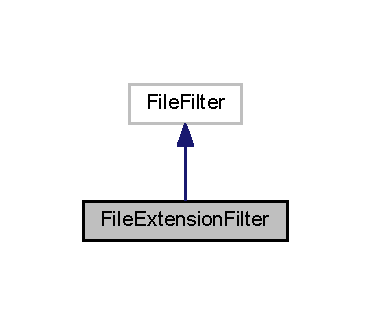
\includegraphics[width=178pt]{classcom_1_1lclion_1_1utils_1_1_file_extension_filter__coll__graph}
\end{center}
\end{figure}
\subsection*{Public Member Functions}
\begin{DoxyCompactItemize}
\item 
\hyperlink{classcom_1_1lclion_1_1utils_1_1_file_extension_filter_a971f3eb77d860e7e40f10ee2ec02bd7a}{File\+Extension\+Filter} (boolean \hyperlink{classcom_1_1lclion_1_1utils_1_1_file_extension_filter_af7a36d46741d21d3e94a00fd0983ff07}{is\+M\+I\+D\+I})
\item 
boolean \hyperlink{classcom_1_1lclion_1_1utils_1_1_file_extension_filter_ab4ef8d92d2363081b9e523ee48ea411c}{accept} (File f)
\item 
String \hyperlink{classcom_1_1lclion_1_1utils_1_1_file_extension_filter_ac7feffb7a33f63504ff1f87f19e2d2d8}{get\+Description} ()
\end{DoxyCompactItemize}
\subsection*{Static Private Attributes}
\begin{DoxyCompactItemize}
\item 
static boolean \hyperlink{classcom_1_1lclion_1_1utils_1_1_file_extension_filter_af7a36d46741d21d3e94a00fd0983ff07}{is\+M\+I\+D\+I} = false
\end{DoxyCompactItemize}


\subsection{Constructor \& Destructor Documentation}
\hypertarget{classcom_1_1lclion_1_1utils_1_1_file_extension_filter_a971f3eb77d860e7e40f10ee2ec02bd7a}{\index{com\+::lclion\+::utils\+::\+File\+Extension\+Filter@{com\+::lclion\+::utils\+::\+File\+Extension\+Filter}!File\+Extension\+Filter@{File\+Extension\+Filter}}
\index{File\+Extension\+Filter@{File\+Extension\+Filter}!com\+::lclion\+::utils\+::\+File\+Extension\+Filter@{com\+::lclion\+::utils\+::\+File\+Extension\+Filter}}
\subsubsection[{File\+Extension\+Filter}]{\setlength{\rightskip}{0pt plus 5cm}{\bf File\+Extension\+Filter} (
\begin{DoxyParamCaption}
\item[{boolean}]{is\+M\+I\+D\+I}
\end{DoxyParamCaption}
)}}\label{classcom_1_1lclion_1_1utils_1_1_file_extension_filter_a971f3eb77d860e7e40f10ee2ec02bd7a}


\subsection{Member Function Documentation}
\hypertarget{classcom_1_1lclion_1_1utils_1_1_file_extension_filter_ab4ef8d92d2363081b9e523ee48ea411c}{\index{com\+::lclion\+::utils\+::\+File\+Extension\+Filter@{com\+::lclion\+::utils\+::\+File\+Extension\+Filter}!accept@{accept}}
\index{accept@{accept}!com\+::lclion\+::utils\+::\+File\+Extension\+Filter@{com\+::lclion\+::utils\+::\+File\+Extension\+Filter}}
\subsubsection[{accept}]{\setlength{\rightskip}{0pt plus 5cm}boolean accept (
\begin{DoxyParamCaption}
\item[{File}]{f}
\end{DoxyParamCaption}
)}}\label{classcom_1_1lclion_1_1utils_1_1_file_extension_filter_ab4ef8d92d2363081b9e523ee48ea411c}


Here is the call graph for this function\+:\nopagebreak
\begin{figure}[H]
\begin{center}
\leavevmode
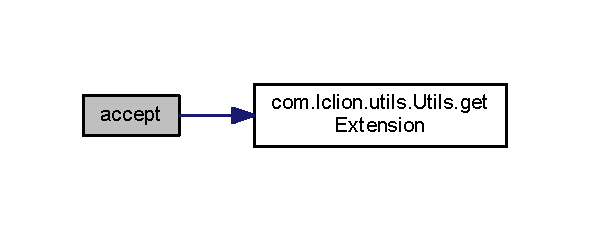
\includegraphics[width=283pt]{classcom_1_1lclion_1_1utils_1_1_file_extension_filter_ab4ef8d92d2363081b9e523ee48ea411c_cgraph}
\end{center}
\end{figure}


\hypertarget{classcom_1_1lclion_1_1utils_1_1_file_extension_filter_ac7feffb7a33f63504ff1f87f19e2d2d8}{\index{com\+::lclion\+::utils\+::\+File\+Extension\+Filter@{com\+::lclion\+::utils\+::\+File\+Extension\+Filter}!get\+Description@{get\+Description}}
\index{get\+Description@{get\+Description}!com\+::lclion\+::utils\+::\+File\+Extension\+Filter@{com\+::lclion\+::utils\+::\+File\+Extension\+Filter}}
\subsubsection[{get\+Description}]{\setlength{\rightskip}{0pt plus 5cm}String get\+Description (
\begin{DoxyParamCaption}
{}
\end{DoxyParamCaption}
)}}\label{classcom_1_1lclion_1_1utils_1_1_file_extension_filter_ac7feffb7a33f63504ff1f87f19e2d2d8}


\subsection{Member Data Documentation}
\hypertarget{classcom_1_1lclion_1_1utils_1_1_file_extension_filter_af7a36d46741d21d3e94a00fd0983ff07}{\index{com\+::lclion\+::utils\+::\+File\+Extension\+Filter@{com\+::lclion\+::utils\+::\+File\+Extension\+Filter}!is\+M\+I\+D\+I@{is\+M\+I\+D\+I}}
\index{is\+M\+I\+D\+I@{is\+M\+I\+D\+I}!com\+::lclion\+::utils\+::\+File\+Extension\+Filter@{com\+::lclion\+::utils\+::\+File\+Extension\+Filter}}
\subsubsection[{is\+M\+I\+D\+I}]{\setlength{\rightskip}{0pt plus 5cm}boolean is\+M\+I\+D\+I = false\hspace{0.3cm}{\ttfamily [static]}, {\ttfamily [private]}}}\label{classcom_1_1lclion_1_1utils_1_1_file_extension_filter_af7a36d46741d21d3e94a00fd0983ff07}


The documentation for this class was generated from the following file\+:\begin{DoxyCompactItemize}
\item 
src/com/lclion/utils/\hyperlink{_file_extension_filter_8java}{File\+Extension\+Filter.\+java}\end{DoxyCompactItemize}

\hypertarget{classcom_1_1lclion_1_1midigui_1_1_init_main}{\section{Init\+Main Class Reference}
\label{classcom_1_1lclion_1_1midigui_1_1_init_main}\index{Init\+Main@{Init\+Main}}
}
\subsection*{Static Public Member Functions}
\begin{DoxyCompactItemize}
\item 
static void \hyperlink{classcom_1_1lclion_1_1midigui_1_1_init_main_a8b260eecbaabcef8473fd87ada040682}{main} (String\mbox{[}$\,$\mbox{]} args)
\end{DoxyCompactItemize}
\subsection*{Static Private Member Functions}
\begin{DoxyCompactItemize}
\item 
static void \hyperlink{classcom_1_1lclion_1_1midigui_1_1_init_main_aeee10cc35bcd0197cf49bc595efc1ea2}{init\+Event\+Dispatch\+Thread} ()
\begin{DoxyCompactList}\small\item\em Initiate the main program. \end{DoxyCompactList}\item 
static void \hyperlink{classcom_1_1lclion_1_1midigui_1_1_init_main_ae9ed8946379ff1f14ef2dab1198a0072}{try\+Look\+And\+Feel} ()
\begin{DoxyCompactList}\small\item\em Attempt to initiate various swing look and feels. \end{DoxyCompactList}\end{DoxyCompactItemize}


\subsection{Detailed Description}
The Main Class. Initialises Java Swing's Look and Feel. Also sets up the Java Swing Event Dispatch Thread (E\+D\+T)

\begin{DoxyAuthor}{Author}
L\+C Lion 
\end{DoxyAuthor}


\subsection{Member Function Documentation}
\hypertarget{classcom_1_1lclion_1_1midigui_1_1_init_main_aeee10cc35bcd0197cf49bc595efc1ea2}{\index{com\+::lclion\+::midigui\+::\+Init\+Main@{com\+::lclion\+::midigui\+::\+Init\+Main}!init\+Event\+Dispatch\+Thread@{init\+Event\+Dispatch\+Thread}}
\index{init\+Event\+Dispatch\+Thread@{init\+Event\+Dispatch\+Thread}!com\+::lclion\+::midigui\+::\+Init\+Main@{com\+::lclion\+::midigui\+::\+Init\+Main}}
\subsubsection[{init\+Event\+Dispatch\+Thread}]{\setlength{\rightskip}{0pt plus 5cm}static void init\+Event\+Dispatch\+Thread (
\begin{DoxyParamCaption}
{}
\end{DoxyParamCaption}
)\hspace{0.3cm}{\ttfamily [static]}, {\ttfamily [private]}}}\label{classcom_1_1lclion_1_1midigui_1_1_init_main_aeee10cc35bcd0197cf49bc595efc1ea2}


Initiate the main program. 

Setup the Java Swing's Event Dispatch Thread and attempt to run the main window. \hypertarget{classcom_1_1lclion_1_1midigui_1_1_init_main_a8b260eecbaabcef8473fd87ada040682}{\index{com\+::lclion\+::midigui\+::\+Init\+Main@{com\+::lclion\+::midigui\+::\+Init\+Main}!main@{main}}
\index{main@{main}!com\+::lclion\+::midigui\+::\+Init\+Main@{com\+::lclion\+::midigui\+::\+Init\+Main}}
\subsubsection[{main}]{\setlength{\rightskip}{0pt plus 5cm}static void main (
\begin{DoxyParamCaption}
\item[{String\mbox{[}$\,$\mbox{]}}]{args}
\end{DoxyParamCaption}
)\hspace{0.3cm}{\ttfamily [static]}}}\label{classcom_1_1lclion_1_1midigui_1_1_init_main_a8b260eecbaabcef8473fd87ada040682}


Here is the call graph for this function\+:\nopagebreak
\begin{figure}[H]
\begin{center}
\leavevmode
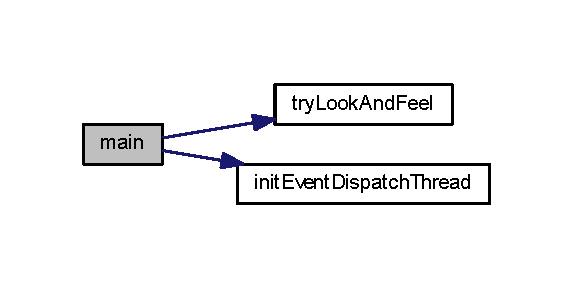
\includegraphics[width=275pt]{classcom_1_1lclion_1_1midigui_1_1_init_main_a8b260eecbaabcef8473fd87ada040682_cgraph}
\end{center}
\end{figure}


\hypertarget{classcom_1_1lclion_1_1midigui_1_1_init_main_ae9ed8946379ff1f14ef2dab1198a0072}{\index{com\+::lclion\+::midigui\+::\+Init\+Main@{com\+::lclion\+::midigui\+::\+Init\+Main}!try\+Look\+And\+Feel@{try\+Look\+And\+Feel}}
\index{try\+Look\+And\+Feel@{try\+Look\+And\+Feel}!com\+::lclion\+::midigui\+::\+Init\+Main@{com\+::lclion\+::midigui\+::\+Init\+Main}}
\subsubsection[{try\+Look\+And\+Feel}]{\setlength{\rightskip}{0pt plus 5cm}static void try\+Look\+And\+Feel (
\begin{DoxyParamCaption}
{}
\end{DoxyParamCaption}
)\hspace{0.3cm}{\ttfamily [static]}, {\ttfamily [private]}}}\label{classcom_1_1lclion_1_1midigui_1_1_init_main_ae9ed8946379ff1f14ef2dab1198a0072}


Attempt to initiate various swing look and feels. 

If the Look and Feel fails for any reason, it will safely fall back to Java Default Look and Feel 

The documentation for this class was generated from the following file\+:\begin{DoxyCompactItemize}
\item 
src/com/lclion/midigui/\hyperlink{_init_main_8java}{Init\+Main.\+java}\end{DoxyCompactItemize}

\hypertarget{classcom_1_1lclion_1_1midigui_1_1_j_frame_m_i_d_i_piano_sheet_creator}{\section{J\+Frame\+M\+I\+D\+I\+Piano\+Sheet\+Creator Class Reference}
\label{classcom_1_1lclion_1_1midigui_1_1_j_frame_m_i_d_i_piano_sheet_creator}\index{J\+Frame\+M\+I\+D\+I\+Piano\+Sheet\+Creator@{J\+Frame\+M\+I\+D\+I\+Piano\+Sheet\+Creator}}
}


The main window of the software.  




Collaboration diagram for J\+Frame\+M\+I\+D\+I\+Piano\+Sheet\+Creator\+:\nopagebreak
\begin{figure}[H]
\begin{center}
\leavevmode
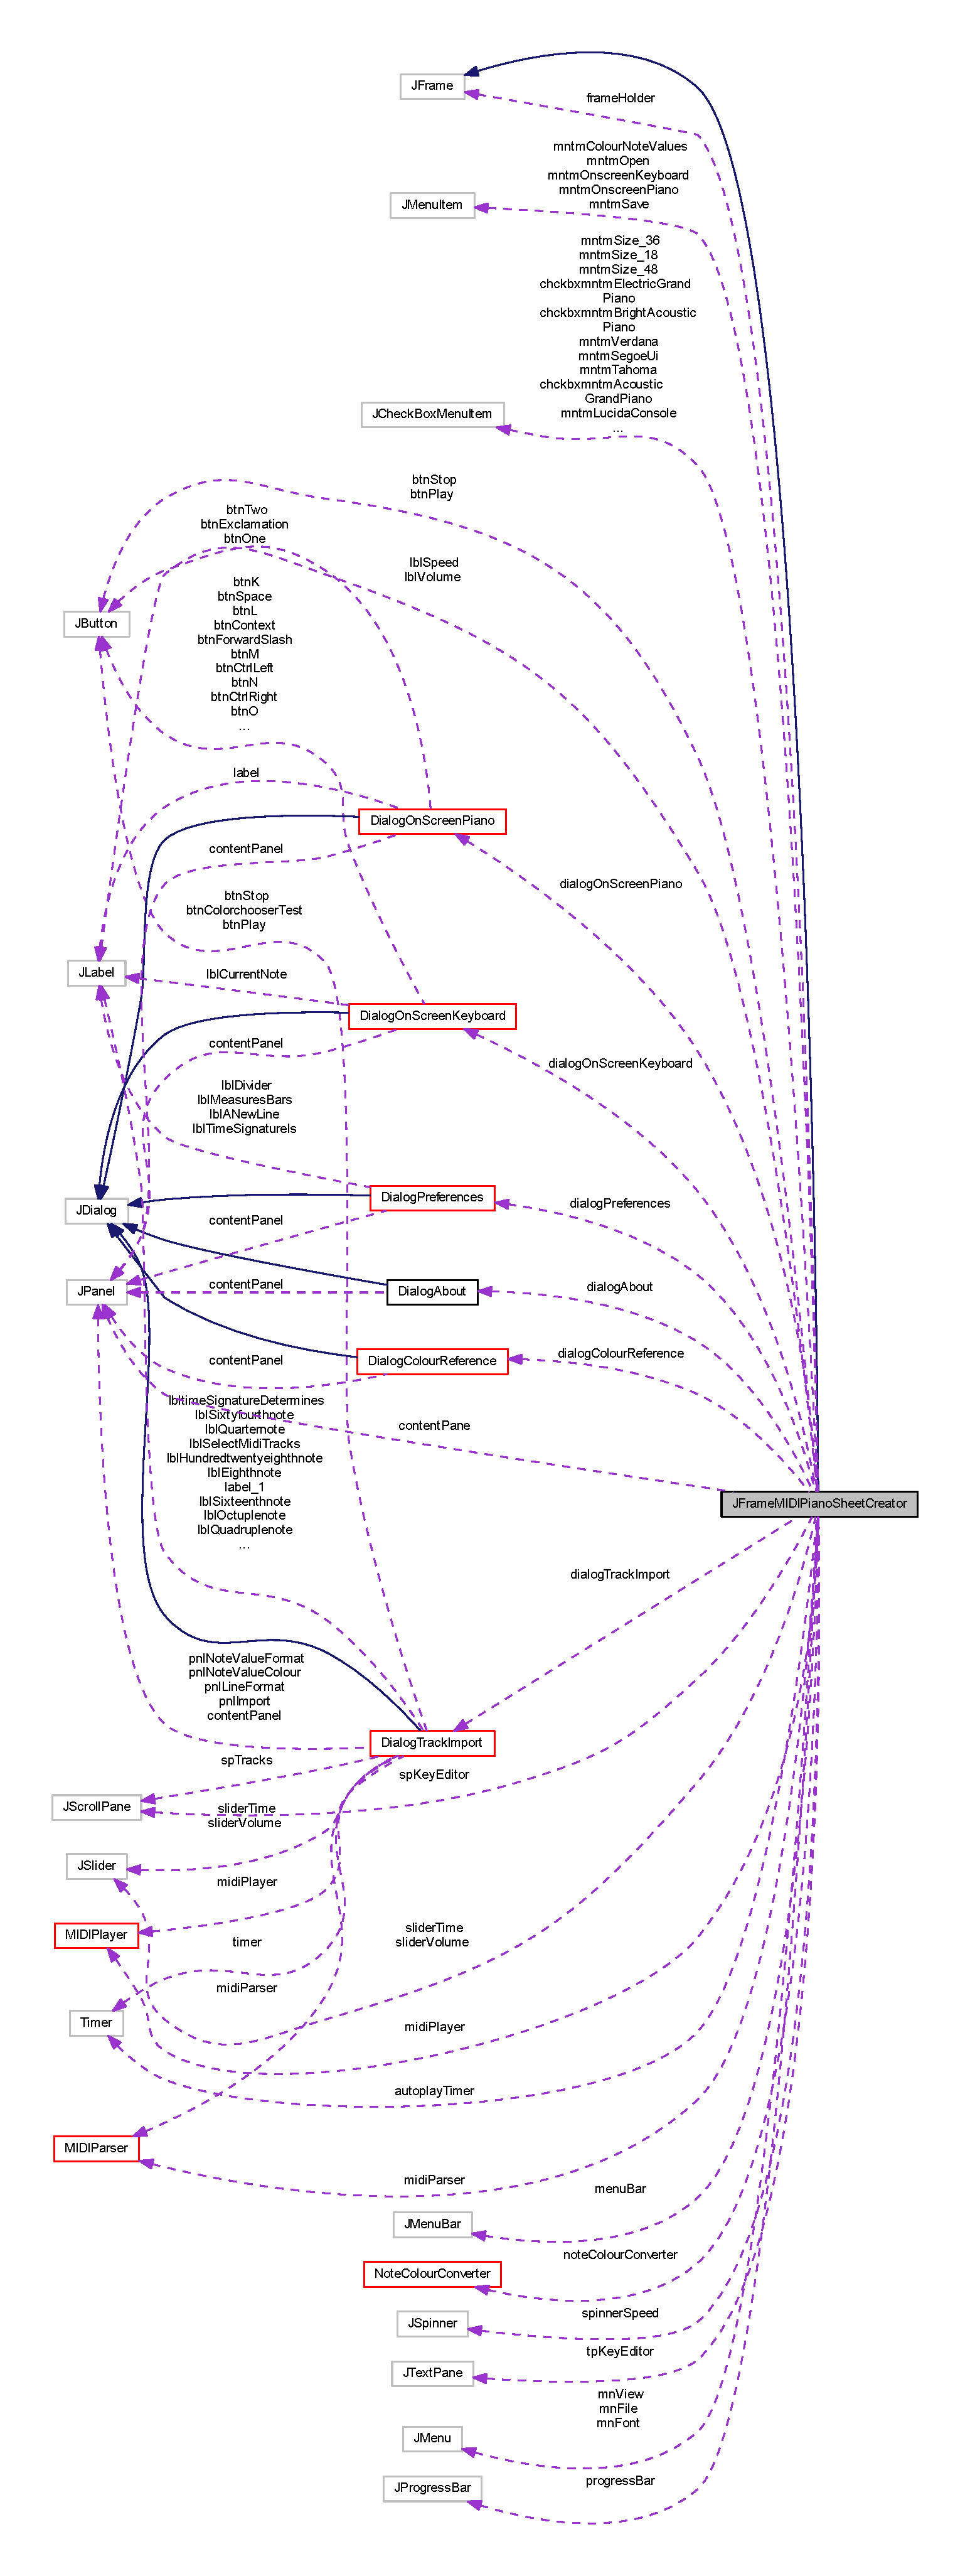
\includegraphics[height=550pt]{classcom_1_1lclion_1_1midigui_1_1_j_frame_m_i_d_i_piano_sheet_creator__coll__graph}
\end{center}
\end{figure}
\subsection*{Package Functions}
\begin{DoxyCompactItemize}
\item 
\hyperlink{classcom_1_1lclion_1_1midigui_1_1_j_frame_m_i_d_i_piano_sheet_creator_aa7344d98b77fcf456e4333719d4e4a34}{J\+Frame\+M\+I\+D\+I\+Piano\+Sheet\+Creator} ()
\end{DoxyCompactItemize}
\subsection*{Private Member Functions}
\begin{DoxyCompactItemize}
\item 
void \hyperlink{classcom_1_1lclion_1_1midigui_1_1_j_frame_m_i_d_i_piano_sheet_creator_a8512e0e195013a23bdecce9bfb93b04c}{init\+Dialogs} ()
\begin{DoxyCompactList}\small\item\em Initialise dialogs related to this window. \end{DoxyCompactList}\item 
void \hyperlink{classcom_1_1lclion_1_1midigui_1_1_j_frame_m_i_d_i_piano_sheet_creator_a27d3ba5afb772cc36c9a432c28975ace}{init\+Buttons} ()
\begin{DoxyCompactList}\small\item\em Initialise buttons related to this window. \end{DoxyCompactList}\item 
void \hyperlink{classcom_1_1lclion_1_1midigui_1_1_j_frame_m_i_d_i_piano_sheet_creator_a2f0269651e213406c54a93a303ef9154}{init\+Button\+Stop} ()
\begin{DoxyCompactList}\small\item\em Initialise the Stop Button and it's event listener. \end{DoxyCompactList}\item 
void \hyperlink{classcom_1_1lclion_1_1midigui_1_1_j_frame_m_i_d_i_piano_sheet_creator_a0251cff1964f088409b3bcb5811f4bc7}{init\+Button\+Play} ()
\begin{DoxyCompactList}\small\item\em Initialise the Play Button and it's event listener. \end{DoxyCompactList}\item 
void \hyperlink{classcom_1_1lclion_1_1midigui_1_1_j_frame_m_i_d_i_piano_sheet_creator_a64517851bfe923ade6f59648b3a9f4e3}{init\+Progress\+Sliders} ()
\begin{DoxyCompactList}\small\item\em Initialise sliders related to this window. \end{DoxyCompactList}\item 
void \hyperlink{classcom_1_1lclion_1_1midigui_1_1_j_frame_m_i_d_i_piano_sheet_creator_af5b3b9751934a25e7d0b73cf458cea99}{init\+Text\+Pane} ()
\begin{DoxyCompactList}\small\item\em Initialise text panes related to this window. \end{DoxyCompactList}\item 
void \hyperlink{classcom_1_1lclion_1_1midigui_1_1_j_frame_m_i_d_i_piano_sheet_creator_ab462219e37674c0df3744f7de1c980ca}{word\+Wrap\+On} ()
\begin{DoxyCompactList}\small\item\em Wordwrap On for text panes related to this window. \end{DoxyCompactList}\item 
void \hyperlink{classcom_1_1lclion_1_1midigui_1_1_j_frame_m_i_d_i_piano_sheet_creator_a42f3eed8a1306302bdebd9dea75883c5}{word\+Wrap\+Off} ()
\begin{DoxyCompactList}\small\item\em Wordwrap Off for text panes related to this window. \end{DoxyCompactList}\item 
void \hyperlink{classcom_1_1lclion_1_1midigui_1_1_j_frame_m_i_d_i_piano_sheet_creator_a0b0e9cd41d19d9cb52443c381a519994}{init\+Menu\+Bar} ()
\begin{DoxyCompactList}\small\item\em Initialise Menu Bars related to this window. \end{DoxyCompactList}\item 
void \hyperlink{classcom_1_1lclion_1_1midigui_1_1_j_frame_m_i_d_i_piano_sheet_creator_a098b454223f052d378bd20af06f6ddf0}{init\+Menu\+Help} ()
\begin{DoxyCompactList}\small\item\em Initialise Menu Help related to this window. \end{DoxyCompactList}\item 
void \hyperlink{classcom_1_1lclion_1_1midigui_1_1_j_frame_m_i_d_i_piano_sheet_creator_a48db1e242ba2acdb007ab6e8f5c245c6}{init\+Menu\+File} ()
\begin{DoxyCompactList}\small\item\em Initialise the menus in the main window. \end{DoxyCompactList}\item 
void \hyperlink{classcom_1_1lclion_1_1midigui_1_1_j_frame_m_i_d_i_piano_sheet_creator_a2b96b6ece7e72836a6e472f85951e297}{init\+Mntm\+Save} ()
\begin{DoxyCompactList}\small\item\em Menu to save the parsed piano sheet to text file (notepad's .txt file format) \end{DoxyCompactList}\item 
void \hyperlink{classcom_1_1lclion_1_1midigui_1_1_j_frame_m_i_d_i_piano_sheet_creator_a6de8f8799e0b919151dd7d602565c867}{init\+Mntm\+Open} ()
\begin{DoxyCompactList}\small\item\em Menu to open a M\+I\+D\+I File. \end{DoxyCompactList}\item 
Swing\+Worker$<$ String, Void $>$ \hyperlink{classcom_1_1lclion_1_1midigui_1_1_j_frame_m_i_d_i_piano_sheet_creator_aae03cd254fec1d9f47948ce62a294baf}{setup\+Swing\+Worker\+M\+I\+D\+I\+Parse} (final File file)
\begin{DoxyCompactList}\small\item\em Returns the Swing\+Worker required to handle M\+I\+D\+I Parsing (Swing\+Worker prevents G\+U\+I freezing) \end{DoxyCompactList}\item 
void \hyperlink{classcom_1_1lclion_1_1midigui_1_1_j_frame_m_i_d_i_piano_sheet_creator_a69eddc42278f45218c12c51637b36d34}{init\+Menu\+Font\+Family} ()
\item 
void \hyperlink{classcom_1_1lclion_1_1midigui_1_1_j_frame_m_i_d_i_piano_sheet_creator_a508329abe82be4cf7842ca7c468f18c8}{init\+Menu\+Font\+Size} ()
\item 
void \hyperlink{classcom_1_1lclion_1_1midigui_1_1_j_frame_m_i_d_i_piano_sheet_creator_a200519724ded34307a2e8c0cd6497a56}{init\+Menu\+Instruments} ()
\item 
void \hyperlink{classcom_1_1lclion_1_1midigui_1_1_j_frame_m_i_d_i_piano_sheet_creator_ae7bd958cecc96a4e5d1ea09834b6d0ef}{change\+Instrument} (int patch\+Num)
\item 
void \hyperlink{classcom_1_1lclion_1_1midigui_1_1_j_frame_m_i_d_i_piano_sheet_creator_ab26c4708edb6e0b42d4988caf68b1ec0}{deselect\+Instrument\+Menu} ()
\item 
void \hyperlink{classcom_1_1lclion_1_1midigui_1_1_j_frame_m_i_d_i_piano_sheet_creator_acb131a460e9412367d53ee82a9375859}{deselect\+Font\+Size\+Menu} ()
\item 
void \hyperlink{classcom_1_1lclion_1_1midigui_1_1_j_frame_m_i_d_i_piano_sheet_creator_a9af7c5fe9801b9b06b53613d2ccd2238}{deselect\+Font\+Family\+Menu} ()
\end{DoxyCompactItemize}
\subsection*{Static Private Member Functions}
\begin{DoxyCompactItemize}
\item 
static void \hyperlink{classcom_1_1lclion_1_1midigui_1_1_j_frame_m_i_d_i_piano_sheet_creator_af20c88021968d70d8665d3664e95a849}{disable\+New\+Folder\+Button} (Container c)
\begin{DoxyCompactList}\small\item\em Disables the \char`\"{}\+New Folder\char`\"{} button when opening files (as it is not necessary) Source\+: java2s.\+com. \end{DoxyCompactList}\end{DoxyCompactItemize}
\subsection*{Private Attributes}
\begin{DoxyCompactItemize}
\item 
J\+Panel \hyperlink{classcom_1_1lclion_1_1midigui_1_1_j_frame_m_i_d_i_piano_sheet_creator_aee369a2eca6b8f16ea106cddf68273e8}{content\+Pane} = null
\item 
J\+Text\+Pane \hyperlink{classcom_1_1lclion_1_1midigui_1_1_j_frame_m_i_d_i_piano_sheet_creator_aa98315e1a5633a11870e6166725b4cd7}{tp\+Key\+Editor}
\item 
J\+Scroll\+Pane \hyperlink{classcom_1_1lclion_1_1midigui_1_1_j_frame_m_i_d_i_piano_sheet_creator_a19fb25d7d050c69ae47f8f492b4de4c8}{sp\+Key\+Editor}
\item 
J\+Menu\+Item \hyperlink{classcom_1_1lclion_1_1midigui_1_1_j_frame_m_i_d_i_piano_sheet_creator_a625ff9936388c864f91a9da3da016101}{mntm\+Save}
\item 
J\+Progress\+Bar \hyperlink{classcom_1_1lclion_1_1midigui_1_1_j_frame_m_i_d_i_piano_sheet_creator_a3fdd66f1536341b66a7bdb456ab2569f}{progress\+Bar}
\item 
J\+Slider \hyperlink{classcom_1_1lclion_1_1midigui_1_1_j_frame_m_i_d_i_piano_sheet_creator_a8f1c2180a937d6483a4912d602dfe023}{slider\+Time}
\item 
J\+Label \hyperlink{classcom_1_1lclion_1_1midigui_1_1_j_frame_m_i_d_i_piano_sheet_creator_aea8fe6af9c54e5d6f1a837809e7e316c}{lbl\+Speed}
\item 
J\+Spinner \hyperlink{classcom_1_1lclion_1_1midigui_1_1_j_frame_m_i_d_i_piano_sheet_creator_a2679c1a277ffcf00ff91ae8bfa676442}{spinner\+Speed}
\item 
J\+Label \hyperlink{classcom_1_1lclion_1_1midigui_1_1_j_frame_m_i_d_i_piano_sheet_creator_a8501b39c874b5ed02e4c630f78aa5de5}{lbl\+Volume}
\item 
J\+Slider \hyperlink{classcom_1_1lclion_1_1midigui_1_1_j_frame_m_i_d_i_piano_sheet_creator_a71f41e4a3f136fb318fb088bd4695dc2}{slider\+Volume}
\item 
J\+Button \hyperlink{classcom_1_1lclion_1_1midigui_1_1_j_frame_m_i_d_i_piano_sheet_creator_aa1718d1d474c9cc2c8f72edef9c6d767}{btn\+Play}
\item 
J\+Button \hyperlink{classcom_1_1lclion_1_1midigui_1_1_j_frame_m_i_d_i_piano_sheet_creator_a3e498460ccccf41b258ee18a8ea8d988}{btn\+Stop}
\item 
\hyperlink{classcom_1_1lclion_1_1midiparser_1_1_m_i_d_i_parser}{M\+I\+D\+I\+Parser} \hyperlink{classcom_1_1lclion_1_1midigui_1_1_j_frame_m_i_d_i_piano_sheet_creator_aba18751017d64d85cea94d280c8e9dc0}{midi\+Parser} = null
\item 
\hyperlink{classcom_1_1lclion_1_1midiplayer_1_1_m_i_d_i_player}{M\+I\+D\+I\+Player} \hyperlink{classcom_1_1lclion_1_1midigui_1_1_j_frame_m_i_d_i_piano_sheet_creator_ab4562caaf138ca21b1013043d3eb158d}{midi\+Player} = null
\item 
\hyperlink{classcom_1_1lclion_1_1midiparser_1_1_note_colour_converter}{Note\+Colour\+Converter} \hyperlink{classcom_1_1lclion_1_1midigui_1_1_j_frame_m_i_d_i_piano_sheet_creator_ab210fa766a5aec2702de6587366989b9}{note\+Colour\+Converter} = null
\item 
String \hyperlink{classcom_1_1lclion_1_1midigui_1_1_j_frame_m_i_d_i_piano_sheet_creator_ae989d6c379f0d116f3811a9d7793e30b}{open\+File\+Name} = null
\item 
String \hyperlink{classcom_1_1lclion_1_1midigui_1_1_j_frame_m_i_d_i_piano_sheet_creator_a1b15f968588be7e6da8f0ffd1c04e6a4}{dir\+File\+Name} = null
\item 
String \hyperlink{classcom_1_1lclion_1_1midigui_1_1_j_frame_m_i_d_i_piano_sheet_creator_a7053fe76095c389b7bbc6d22f2ba5b21}{last\+Directory} = null
\item 
String \hyperlink{classcom_1_1lclion_1_1midigui_1_1_j_frame_m_i_d_i_piano_sheet_creator_a62123d133e7e491e26258033b8b08822}{current\+Font} = \char`\"{}Verdana\char`\"{}
\item 
int \hyperlink{classcom_1_1lclion_1_1midigui_1_1_j_frame_m_i_d_i_piano_sheet_creator_a7f8543b687b957a013ba58ffdd9449f2}{current\+Font\+Size} = 12
\item 
Timer \hyperlink{classcom_1_1lclion_1_1midigui_1_1_j_frame_m_i_d_i_piano_sheet_creator_a172d0561900ff10f21cbf9562fa3c261}{autoplay\+Timer} = null
\item 
int \hyperlink{classcom_1_1lclion_1_1midigui_1_1_j_frame_m_i_d_i_piano_sheet_creator_aa6ae8f708b6cde0c380df6aea7059360}{current\+Patch\+Num} = -\/1
\item 
J\+Menu\+Bar \hyperlink{classcom_1_1lclion_1_1midigui_1_1_j_frame_m_i_d_i_piano_sheet_creator_a654581aa0d77b3f6860722adc9d9fc1d}{menu\+Bar}
\item 
J\+Menu \hyperlink{classcom_1_1lclion_1_1midigui_1_1_j_frame_m_i_d_i_piano_sheet_creator_adc23b01d38b600ce897d16e596c2b868}{mn\+Font}
\item 
J\+Check\+Box\+Menu\+Item \hyperlink{classcom_1_1lclion_1_1midigui_1_1_j_frame_m_i_d_i_piano_sheet_creator_acf27febb9f46a2cb5b78ecb7e283e243}{chckbxmntm\+Acoustic\+Grand\+Piano}
\item 
J\+Check\+Box\+Menu\+Item \hyperlink{classcom_1_1lclion_1_1midigui_1_1_j_frame_m_i_d_i_piano_sheet_creator_aafdf4f78ebd2521a1ec7f34e1e06e4a9}{chckbxmntm\+Bright\+Acoustic\+Piano}
\item 
J\+Check\+Box\+Menu\+Item \hyperlink{classcom_1_1lclion_1_1midigui_1_1_j_frame_m_i_d_i_piano_sheet_creator_ade34b598a3fb7ba9a61e9b2b7687ad9e}{chckbxmntm\+Electric\+Grand\+Piano}
\item 
J\+Check\+Box\+Menu\+Item \hyperlink{classcom_1_1lclion_1_1midigui_1_1_j_frame_m_i_d_i_piano_sheet_creator_ac9819205c38c3591401116984553387e}{chckbxmntm\+Use\+Midi\+Default}
\item 
J\+Check\+Box\+Menu\+Item \hyperlink{classcom_1_1lclion_1_1midigui_1_1_j_frame_m_i_d_i_piano_sheet_creator_ab59060cc1aaa1acf916f717203b8c8bd}{chckbxmntm\+Honky\+Tonk\+Piano}
\item 
J\+Check\+Box\+Menu\+Item \hyperlink{classcom_1_1lclion_1_1midigui_1_1_j_frame_m_i_d_i_piano_sheet_creator_a2a76124f85968992b142ad2d9fc78c73}{chckbxmntm\+Electric\+Piano1}
\item 
J\+Check\+Box\+Menu\+Item \hyperlink{classcom_1_1lclion_1_1midigui_1_1_j_frame_m_i_d_i_piano_sheet_creator_a64bf84906a571db4297425d89fd61dbd}{chckbxmntm\+Electric\+Piano2}
\item 
J\+Check\+Box\+Menu\+Item \hyperlink{classcom_1_1lclion_1_1midigui_1_1_j_frame_m_i_d_i_piano_sheet_creator_ad63305d8ca6fab38cf74a892d780461c}{chckbxmntm\+Harpsichord}
\item 
J\+Check\+Box\+Menu\+Item \hyperlink{classcom_1_1lclion_1_1midigui_1_1_j_frame_m_i_d_i_piano_sheet_creator_a1eba3e74979ed3e70114af6927e625a4}{chckbxmntm\+Clavinet}
\item 
J\+Check\+Box\+Menu\+Item \hyperlink{classcom_1_1lclion_1_1midigui_1_1_j_frame_m_i_d_i_piano_sheet_creator_ae16ca66c315ae28ba7b99aad21ad5e09}{mntm\+Size\+\_\+8}
\item 
J\+Check\+Box\+Menu\+Item \hyperlink{classcom_1_1lclion_1_1midigui_1_1_j_frame_m_i_d_i_piano_sheet_creator_a3c49956bedee4fd23f4986f598da688c}{mntm\+Size\+\_\+10}
\item 
J\+Check\+Box\+Menu\+Item \hyperlink{classcom_1_1lclion_1_1midigui_1_1_j_frame_m_i_d_i_piano_sheet_creator_ada6afb80750b1367cbb4dc4acae49f4b}{mntm\+Size\+\_\+12}
\item 
J\+Check\+Box\+Menu\+Item \hyperlink{classcom_1_1lclion_1_1midigui_1_1_j_frame_m_i_d_i_piano_sheet_creator_afe11959823d15698b8ef79c701d24705}{mntm\+Size\+\_\+14}
\item 
J\+Check\+Box\+Menu\+Item \hyperlink{classcom_1_1lclion_1_1midigui_1_1_j_frame_m_i_d_i_piano_sheet_creator_ad753490ecc6eb30372c7e8a4d9bce319}{mntm\+Size\+\_\+16}
\item 
J\+Check\+Box\+Menu\+Item \hyperlink{classcom_1_1lclion_1_1midigui_1_1_j_frame_m_i_d_i_piano_sheet_creator_ae3c577e710806d61ed05df0bc8be487b}{mntm\+Size\+\_\+18}
\item 
J\+Check\+Box\+Menu\+Item \hyperlink{classcom_1_1lclion_1_1midigui_1_1_j_frame_m_i_d_i_piano_sheet_creator_a97a4d037ea3a2b0a556280f5fc90fc01}{mntm\+Size\+\_\+24}
\item 
J\+Check\+Box\+Menu\+Item \hyperlink{classcom_1_1lclion_1_1midigui_1_1_j_frame_m_i_d_i_piano_sheet_creator_a325e2a4cd1cd58269d9f8b3957a09710}{mntm\+Size\+\_\+36}
\item 
J\+Check\+Box\+Menu\+Item \hyperlink{classcom_1_1lclion_1_1midigui_1_1_j_frame_m_i_d_i_piano_sheet_creator_a8aadd2c41e4cca1d9cd36676f10a7b4c}{mntm\+Size\+\_\+48}
\item 
J\+Check\+Box\+Menu\+Item \hyperlink{classcom_1_1lclion_1_1midigui_1_1_j_frame_m_i_d_i_piano_sheet_creator_acd08c18bd1a4b76d59dc747cc2cb416a}{mntm\+Lucida\+Console}
\item 
J\+Check\+Box\+Menu\+Item \hyperlink{classcom_1_1lclion_1_1midigui_1_1_j_frame_m_i_d_i_piano_sheet_creator_aa7eb8b768edb92241a98e41f17cd6570}{mntm\+Tahoma}
\item 
J\+Check\+Box\+Menu\+Item \hyperlink{classcom_1_1lclion_1_1midigui_1_1_j_frame_m_i_d_i_piano_sheet_creator_a05f0a24d3f92ed2dbbfe7eced7c05b12}{mntm\+Verdana}
\item 
J\+Check\+Box\+Menu\+Item \hyperlink{classcom_1_1lclion_1_1midigui_1_1_j_frame_m_i_d_i_piano_sheet_creator_aa9eb27d5b6fea0c0835a299547f1d676}{mntm\+Segoe\+Ui}
\item 
J\+Menu \hyperlink{classcom_1_1lclion_1_1midigui_1_1_j_frame_m_i_d_i_piano_sheet_creator_a5bdad6dc2b9da47a45a0a6b1454b85ed}{mn\+View}
\item 
J\+Menu\+Item \hyperlink{classcom_1_1lclion_1_1midigui_1_1_j_frame_m_i_d_i_piano_sheet_creator_ab94476c50fe222e692fa9339ac3ec45f}{mntm\+Colour\+Note\+Values}
\item 
J\+Menu\+Item \hyperlink{classcom_1_1lclion_1_1midigui_1_1_j_frame_m_i_d_i_piano_sheet_creator_a772d6e85bb1207eda7775a39e8b8d2a7}{mntm\+Onscreen\+Keyboard}
\item 
J\+Menu\+Item \hyperlink{classcom_1_1lclion_1_1midigui_1_1_j_frame_m_i_d_i_piano_sheet_creator_a41b99c6291375c2f6ca410c5819d0c26}{mntm\+Onscreen\+Piano}
\item 
J\+Menu \hyperlink{classcom_1_1lclion_1_1midigui_1_1_j_frame_m_i_d_i_piano_sheet_creator_a48cc7fde4429ea728b772b1c8ef965df}{mn\+File}
\end{DoxyCompactItemize}
\subsection*{Static Private Attributes}
\begin{DoxyCompactItemize}
\item 
static J\+Frame \hyperlink{classcom_1_1lclion_1_1midigui_1_1_j_frame_m_i_d_i_piano_sheet_creator_acbbeb368af441422247853ca2d6641c4}{frame\+Holder} = null
\item 
static J\+Menu\+Item \hyperlink{classcom_1_1lclion_1_1midigui_1_1_j_frame_m_i_d_i_piano_sheet_creator_a96b3e2db6919b4449aca72fc9a20b980}{mntm\+Open}
\item 
static \hyperlink{classcom_1_1lclion_1_1midigui_1_1_dialog_about}{Dialog\+About} \hyperlink{classcom_1_1lclion_1_1midigui_1_1_j_frame_m_i_d_i_piano_sheet_creator_a047d953d878b28ab2a2807642ea76766}{dialog\+About} = null
\item 
static \hyperlink{classcom_1_1lclion_1_1midigui_1_1_dialog_preferences}{Dialog\+Preferences} \hyperlink{classcom_1_1lclion_1_1midigui_1_1_j_frame_m_i_d_i_piano_sheet_creator_ab8f21a3b29b7b03f47d37ab0be98d7a5}{dialog\+Preferences} = null
\item 
static \hyperlink{classcom_1_1lclion_1_1midigui_1_1_dialog_track_import}{Dialog\+Track\+Import} \hyperlink{classcom_1_1lclion_1_1midigui_1_1_j_frame_m_i_d_i_piano_sheet_creator_a779c5b2f4e1dcc94515f3e174380101c}{dialog\+Track\+Import} = null
\item 
static \hyperlink{classcom_1_1lclion_1_1midigui_1_1_dialog_colour_reference}{Dialog\+Colour\+Reference} \hyperlink{classcom_1_1lclion_1_1midigui_1_1_j_frame_m_i_d_i_piano_sheet_creator_ab5e923b68d49fe2353d6b88660db06d5}{dialog\+Colour\+Reference} = null
\item 
static \hyperlink{classcom_1_1lclion_1_1midigui_1_1_dialog_on_screen_keyboard}{Dialog\+On\+Screen\+Keyboard} \hyperlink{classcom_1_1lclion_1_1midigui_1_1_j_frame_m_i_d_i_piano_sheet_creator_a381bf6ccecb17ef281f31251e09e2a10}{dialog\+On\+Screen\+Keyboard} = null
\item 
static \hyperlink{classcom_1_1lclion_1_1midigui_1_1_dialog_on_screen_piano}{Dialog\+On\+Screen\+Piano} \hyperlink{classcom_1_1lclion_1_1midigui_1_1_j_frame_m_i_d_i_piano_sheet_creator_a03a695600b98ed60aef1c2d5339abcf9}{dialog\+On\+Screen\+Piano} = null
\end{DoxyCompactItemize}


\subsection{Detailed Description}
The main window of the software. 

Initialises all of G\+U\+I Java Swing components as well as other Dialog Classes.

Some components have Event Listeners which includes the code logic in them.

\begin{DoxyAuthor}{Author}
L\+C Lion 
\end{DoxyAuthor}


\subsection{Constructor \& Destructor Documentation}
\hypertarget{classcom_1_1lclion_1_1midigui_1_1_j_frame_m_i_d_i_piano_sheet_creator_aa7344d98b77fcf456e4333719d4e4a34}{\index{com\+::lclion\+::midigui\+::\+J\+Frame\+M\+I\+D\+I\+Piano\+Sheet\+Creator@{com\+::lclion\+::midigui\+::\+J\+Frame\+M\+I\+D\+I\+Piano\+Sheet\+Creator}!J\+Frame\+M\+I\+D\+I\+Piano\+Sheet\+Creator@{J\+Frame\+M\+I\+D\+I\+Piano\+Sheet\+Creator}}
\index{J\+Frame\+M\+I\+D\+I\+Piano\+Sheet\+Creator@{J\+Frame\+M\+I\+D\+I\+Piano\+Sheet\+Creator}!com\+::lclion\+::midigui\+::\+J\+Frame\+M\+I\+D\+I\+Piano\+Sheet\+Creator@{com\+::lclion\+::midigui\+::\+J\+Frame\+M\+I\+D\+I\+Piano\+Sheet\+Creator}}
\subsubsection[{J\+Frame\+M\+I\+D\+I\+Piano\+Sheet\+Creator}]{\setlength{\rightskip}{0pt plus 5cm}{\bf J\+Frame\+M\+I\+D\+I\+Piano\+Sheet\+Creator} (
\begin{DoxyParamCaption}
{}
\end{DoxyParamCaption}
)\hspace{0.3cm}{\ttfamily [package]}}}\label{classcom_1_1lclion_1_1midigui_1_1_j_frame_m_i_d_i_piano_sheet_creator_aa7344d98b77fcf456e4333719d4e4a34}
Constructor that initialises all G\+U\+I components and it's Event Listeners.

This class is run under Java Swing's Event Dispatch Thread, and is not thread safe.

Use Swing\+Worker class to do lengthy operations, else the G\+U\+I will freeze. 

Here is the call graph for this function\+:
\nopagebreak
\begin{figure}[H]
\begin{center}
\leavevmode
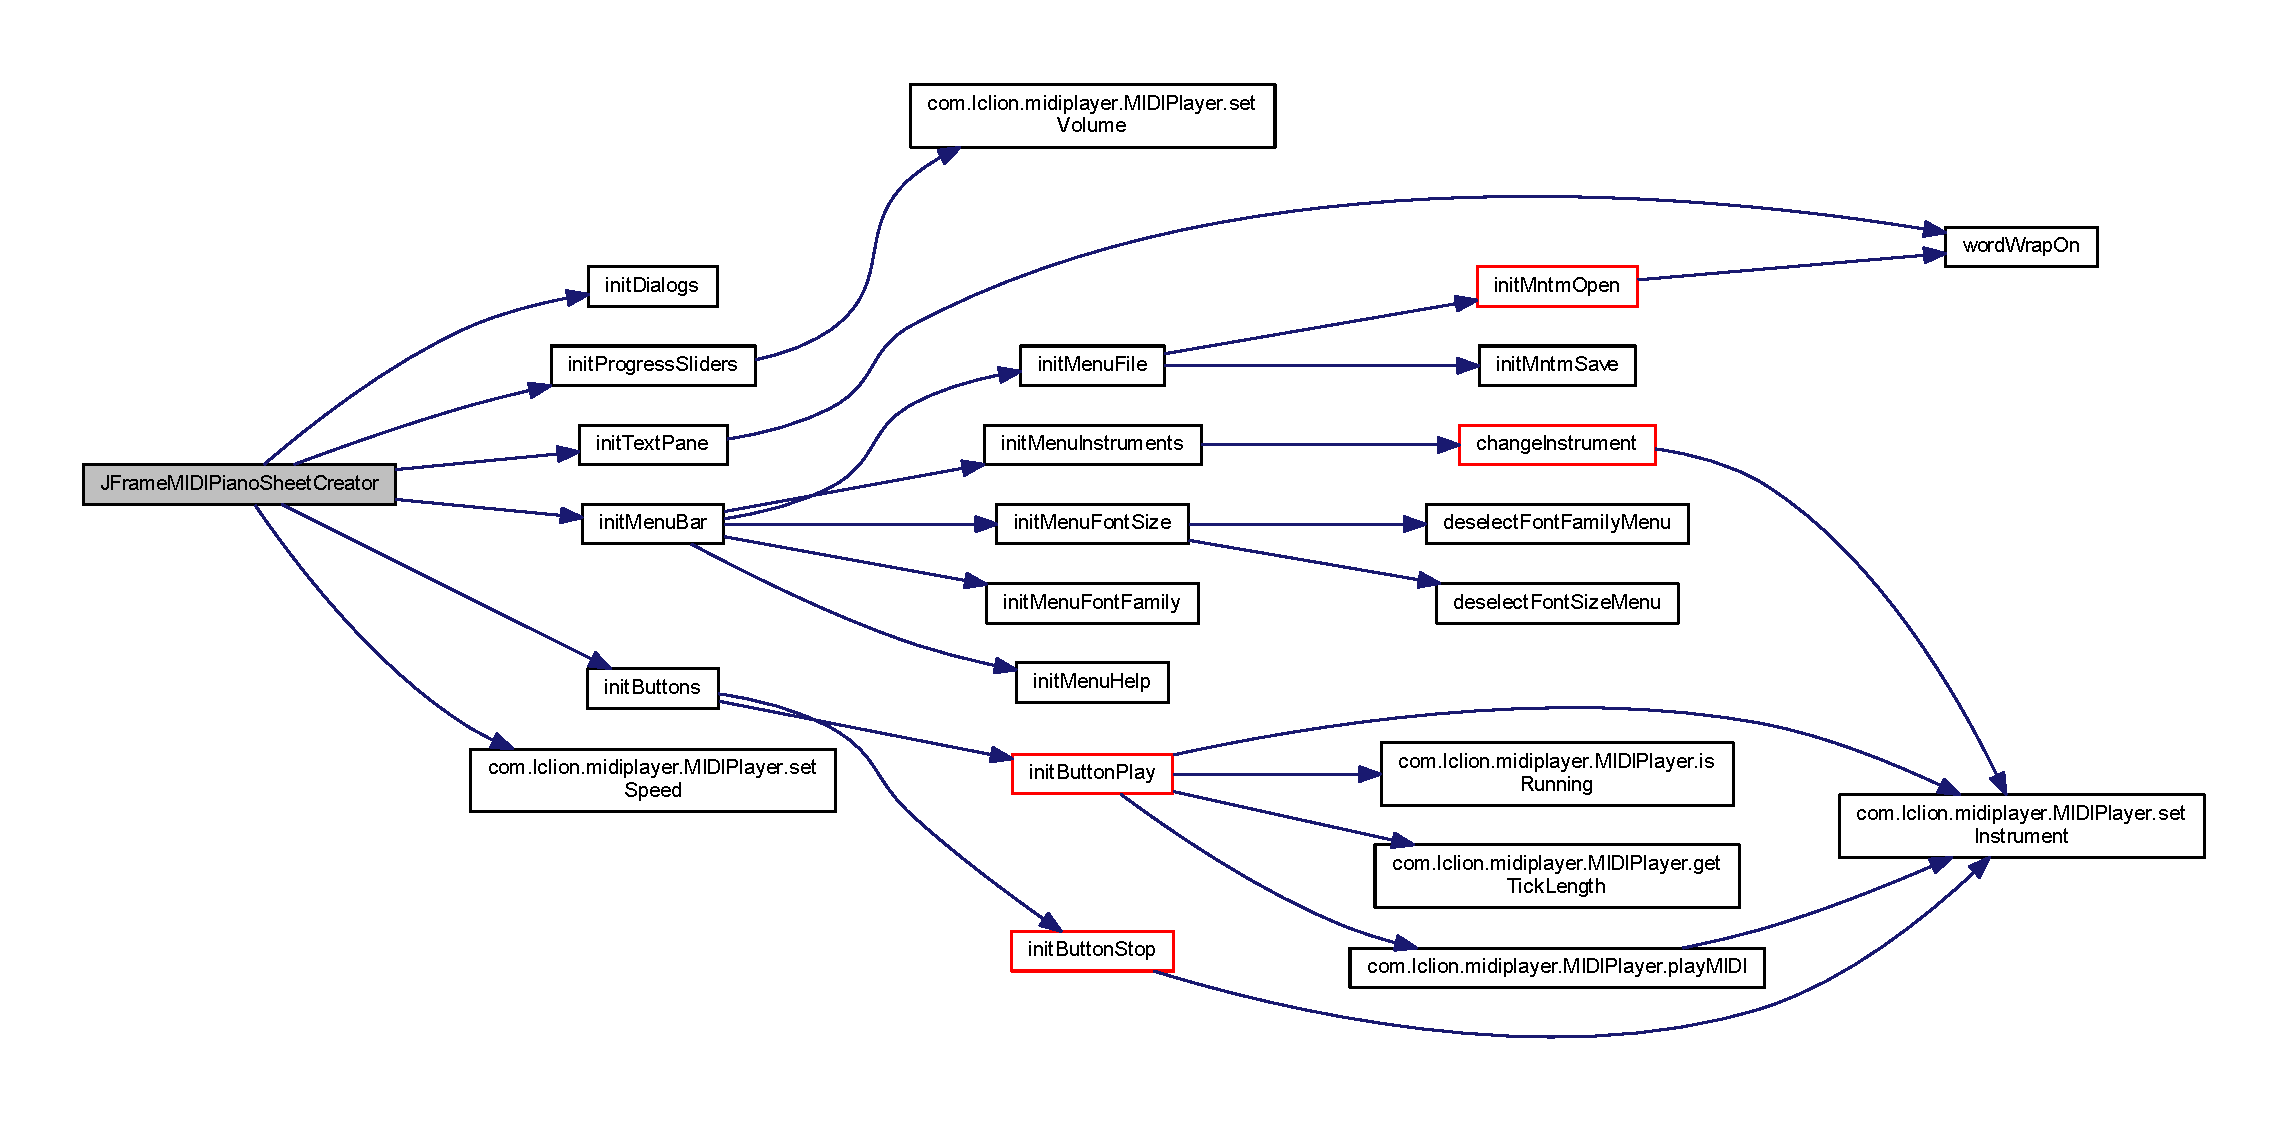
\includegraphics[width=350pt]{classcom_1_1lclion_1_1midigui_1_1_j_frame_m_i_d_i_piano_sheet_creator_aa7344d98b77fcf456e4333719d4e4a34_cgraph}
\end{center}
\end{figure}




\subsection{Member Function Documentation}
\hypertarget{classcom_1_1lclion_1_1midigui_1_1_j_frame_m_i_d_i_piano_sheet_creator_ae7bd958cecc96a4e5d1ea09834b6d0ef}{\index{com\+::lclion\+::midigui\+::\+J\+Frame\+M\+I\+D\+I\+Piano\+Sheet\+Creator@{com\+::lclion\+::midigui\+::\+J\+Frame\+M\+I\+D\+I\+Piano\+Sheet\+Creator}!change\+Instrument@{change\+Instrument}}
\index{change\+Instrument@{change\+Instrument}!com\+::lclion\+::midigui\+::\+J\+Frame\+M\+I\+D\+I\+Piano\+Sheet\+Creator@{com\+::lclion\+::midigui\+::\+J\+Frame\+M\+I\+D\+I\+Piano\+Sheet\+Creator}}
\subsubsection[{change\+Instrument}]{\setlength{\rightskip}{0pt plus 5cm}void change\+Instrument (
\begin{DoxyParamCaption}
\item[{int}]{patch\+Num}
\end{DoxyParamCaption}
)\hspace{0.3cm}{\ttfamily [private]}}}\label{classcom_1_1lclion_1_1midigui_1_1_j_frame_m_i_d_i_piano_sheet_creator_ae7bd958cecc96a4e5d1ea09834b6d0ef}


Here is the call graph for this function\+:\nopagebreak
\begin{figure}[H]
\begin{center}
\leavevmode
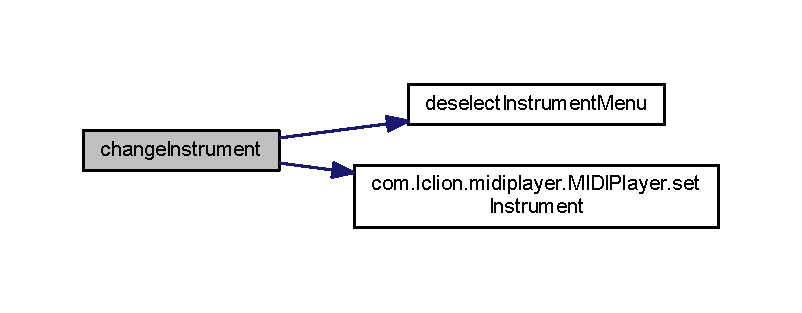
\includegraphics[width=350pt]{classcom_1_1lclion_1_1midigui_1_1_j_frame_m_i_d_i_piano_sheet_creator_ae7bd958cecc96a4e5d1ea09834b6d0ef_cgraph}
\end{center}
\end{figure}


\hypertarget{classcom_1_1lclion_1_1midigui_1_1_j_frame_m_i_d_i_piano_sheet_creator_a9af7c5fe9801b9b06b53613d2ccd2238}{\index{com\+::lclion\+::midigui\+::\+J\+Frame\+M\+I\+D\+I\+Piano\+Sheet\+Creator@{com\+::lclion\+::midigui\+::\+J\+Frame\+M\+I\+D\+I\+Piano\+Sheet\+Creator}!deselect\+Font\+Family\+Menu@{deselect\+Font\+Family\+Menu}}
\index{deselect\+Font\+Family\+Menu@{deselect\+Font\+Family\+Menu}!com\+::lclion\+::midigui\+::\+J\+Frame\+M\+I\+D\+I\+Piano\+Sheet\+Creator@{com\+::lclion\+::midigui\+::\+J\+Frame\+M\+I\+D\+I\+Piano\+Sheet\+Creator}}
\subsubsection[{deselect\+Font\+Family\+Menu}]{\setlength{\rightskip}{0pt plus 5cm}void deselect\+Font\+Family\+Menu (
\begin{DoxyParamCaption}
{}
\end{DoxyParamCaption}
)\hspace{0.3cm}{\ttfamily [private]}}}\label{classcom_1_1lclion_1_1midigui_1_1_j_frame_m_i_d_i_piano_sheet_creator_a9af7c5fe9801b9b06b53613d2ccd2238}
\hypertarget{classcom_1_1lclion_1_1midigui_1_1_j_frame_m_i_d_i_piano_sheet_creator_acb131a460e9412367d53ee82a9375859}{\index{com\+::lclion\+::midigui\+::\+J\+Frame\+M\+I\+D\+I\+Piano\+Sheet\+Creator@{com\+::lclion\+::midigui\+::\+J\+Frame\+M\+I\+D\+I\+Piano\+Sheet\+Creator}!deselect\+Font\+Size\+Menu@{deselect\+Font\+Size\+Menu}}
\index{deselect\+Font\+Size\+Menu@{deselect\+Font\+Size\+Menu}!com\+::lclion\+::midigui\+::\+J\+Frame\+M\+I\+D\+I\+Piano\+Sheet\+Creator@{com\+::lclion\+::midigui\+::\+J\+Frame\+M\+I\+D\+I\+Piano\+Sheet\+Creator}}
\subsubsection[{deselect\+Font\+Size\+Menu}]{\setlength{\rightskip}{0pt plus 5cm}void deselect\+Font\+Size\+Menu (
\begin{DoxyParamCaption}
{}
\end{DoxyParamCaption}
)\hspace{0.3cm}{\ttfamily [private]}}}\label{classcom_1_1lclion_1_1midigui_1_1_j_frame_m_i_d_i_piano_sheet_creator_acb131a460e9412367d53ee82a9375859}
\hypertarget{classcom_1_1lclion_1_1midigui_1_1_j_frame_m_i_d_i_piano_sheet_creator_ab26c4708edb6e0b42d4988caf68b1ec0}{\index{com\+::lclion\+::midigui\+::\+J\+Frame\+M\+I\+D\+I\+Piano\+Sheet\+Creator@{com\+::lclion\+::midigui\+::\+J\+Frame\+M\+I\+D\+I\+Piano\+Sheet\+Creator}!deselect\+Instrument\+Menu@{deselect\+Instrument\+Menu}}
\index{deselect\+Instrument\+Menu@{deselect\+Instrument\+Menu}!com\+::lclion\+::midigui\+::\+J\+Frame\+M\+I\+D\+I\+Piano\+Sheet\+Creator@{com\+::lclion\+::midigui\+::\+J\+Frame\+M\+I\+D\+I\+Piano\+Sheet\+Creator}}
\subsubsection[{deselect\+Instrument\+Menu}]{\setlength{\rightskip}{0pt plus 5cm}void deselect\+Instrument\+Menu (
\begin{DoxyParamCaption}
{}
\end{DoxyParamCaption}
)\hspace{0.3cm}{\ttfamily [private]}}}\label{classcom_1_1lclion_1_1midigui_1_1_j_frame_m_i_d_i_piano_sheet_creator_ab26c4708edb6e0b42d4988caf68b1ec0}
\hypertarget{classcom_1_1lclion_1_1midigui_1_1_j_frame_m_i_d_i_piano_sheet_creator_af20c88021968d70d8665d3664e95a849}{\index{com\+::lclion\+::midigui\+::\+J\+Frame\+M\+I\+D\+I\+Piano\+Sheet\+Creator@{com\+::lclion\+::midigui\+::\+J\+Frame\+M\+I\+D\+I\+Piano\+Sheet\+Creator}!disable\+New\+Folder\+Button@{disable\+New\+Folder\+Button}}
\index{disable\+New\+Folder\+Button@{disable\+New\+Folder\+Button}!com\+::lclion\+::midigui\+::\+J\+Frame\+M\+I\+D\+I\+Piano\+Sheet\+Creator@{com\+::lclion\+::midigui\+::\+J\+Frame\+M\+I\+D\+I\+Piano\+Sheet\+Creator}}
\subsubsection[{disable\+New\+Folder\+Button}]{\setlength{\rightskip}{0pt plus 5cm}static void disable\+New\+Folder\+Button (
\begin{DoxyParamCaption}
\item[{Container}]{c}
\end{DoxyParamCaption}
)\hspace{0.3cm}{\ttfamily [static]}, {\ttfamily [private]}}}\label{classcom_1_1lclion_1_1midigui_1_1_j_frame_m_i_d_i_piano_sheet_creator_af20c88021968d70d8665d3664e95a849}


Disables the \char`\"{}\+New Folder\char`\"{} button when opening files (as it is not necessary) Source\+: java2s.\+com. 


\begin{DoxyParams}{Parameters}
{\em c} & The container which has the component needed to search and disable the \char`\"{}\+New Folder\char`\"{} button \\
\hline
\end{DoxyParams}
\hypertarget{classcom_1_1lclion_1_1midigui_1_1_j_frame_m_i_d_i_piano_sheet_creator_a0251cff1964f088409b3bcb5811f4bc7}{\index{com\+::lclion\+::midigui\+::\+J\+Frame\+M\+I\+D\+I\+Piano\+Sheet\+Creator@{com\+::lclion\+::midigui\+::\+J\+Frame\+M\+I\+D\+I\+Piano\+Sheet\+Creator}!init\+Button\+Play@{init\+Button\+Play}}
\index{init\+Button\+Play@{init\+Button\+Play}!com\+::lclion\+::midigui\+::\+J\+Frame\+M\+I\+D\+I\+Piano\+Sheet\+Creator@{com\+::lclion\+::midigui\+::\+J\+Frame\+M\+I\+D\+I\+Piano\+Sheet\+Creator}}
\subsubsection[{init\+Button\+Play}]{\setlength{\rightskip}{0pt plus 5cm}void init\+Button\+Play (
\begin{DoxyParamCaption}
{}
\end{DoxyParamCaption}
)\hspace{0.3cm}{\ttfamily [private]}}}\label{classcom_1_1lclion_1_1midigui_1_1_j_frame_m_i_d_i_piano_sheet_creator_a0251cff1964f088409b3bcb5811f4bc7}


Initialise the Play Button and it's event listener. 

Plays the current M\+I\+D\+I File loaded.

The action listener for this button also triggers the auto highlighting feature on the textpane. 

Here is the call graph for this function\+:\nopagebreak
\begin{figure}[H]
\begin{center}
\leavevmode
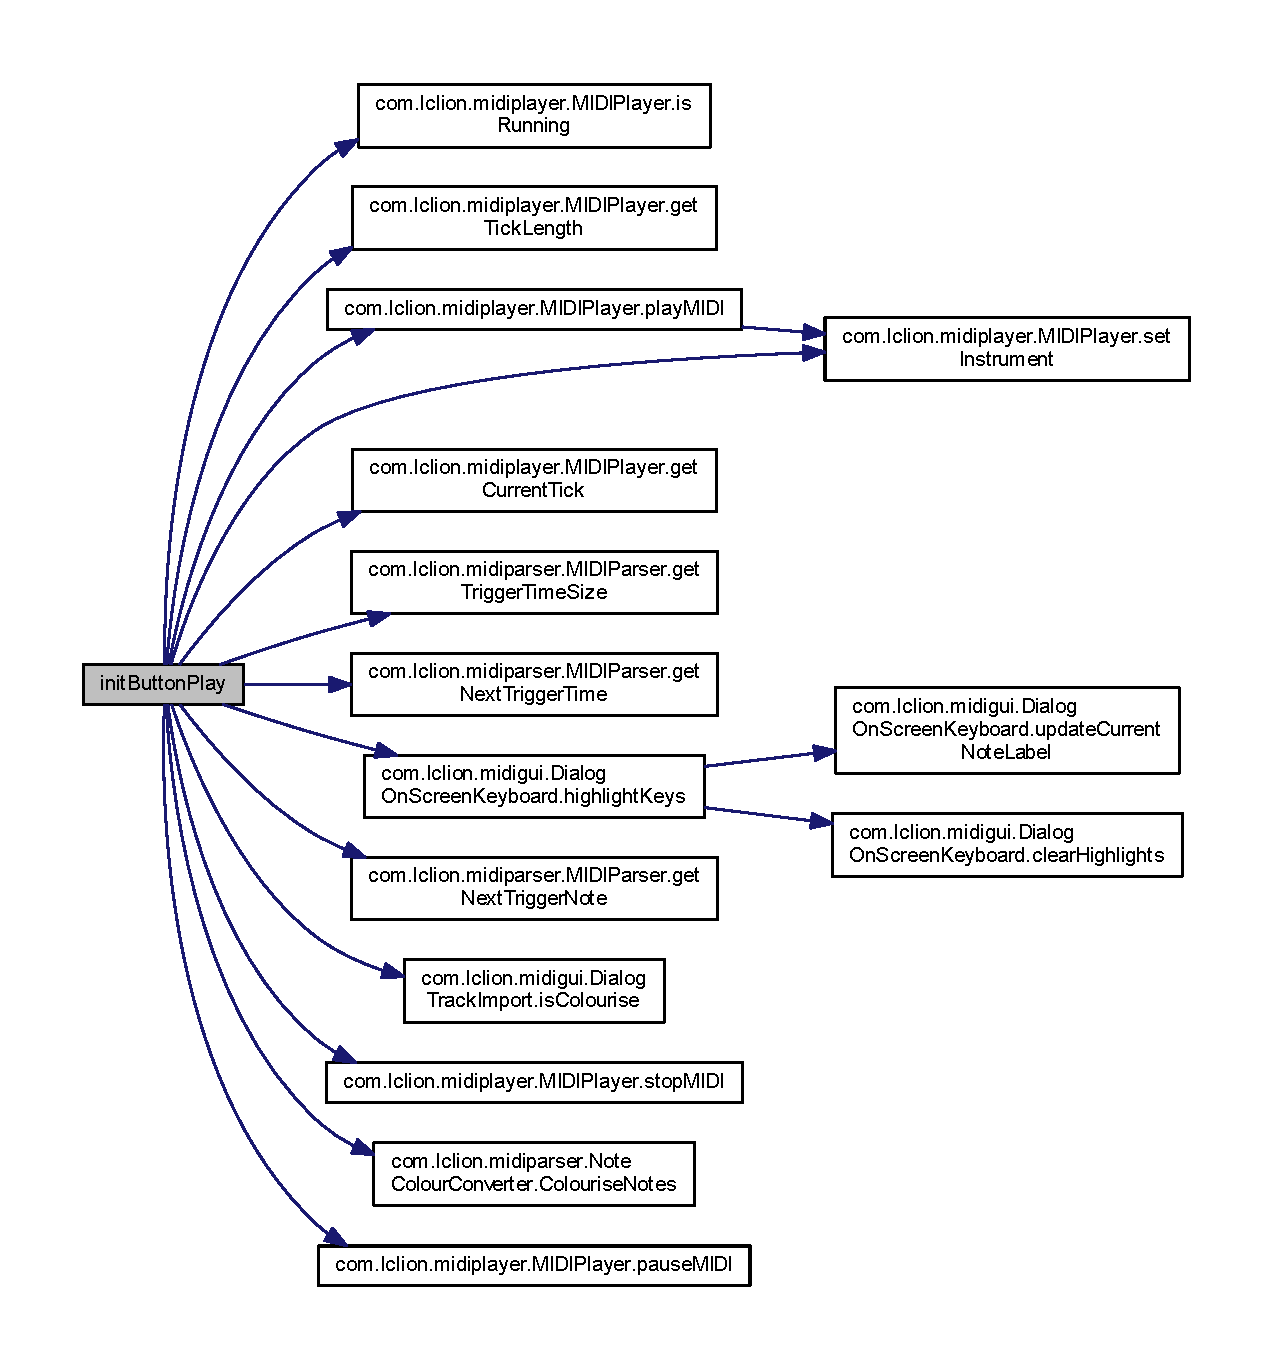
\includegraphics[width=350pt]{classcom_1_1lclion_1_1midigui_1_1_j_frame_m_i_d_i_piano_sheet_creator_a0251cff1964f088409b3bcb5811f4bc7_cgraph}
\end{center}
\end{figure}


\hypertarget{classcom_1_1lclion_1_1midigui_1_1_j_frame_m_i_d_i_piano_sheet_creator_a27d3ba5afb772cc36c9a432c28975ace}{\index{com\+::lclion\+::midigui\+::\+J\+Frame\+M\+I\+D\+I\+Piano\+Sheet\+Creator@{com\+::lclion\+::midigui\+::\+J\+Frame\+M\+I\+D\+I\+Piano\+Sheet\+Creator}!init\+Buttons@{init\+Buttons}}
\index{init\+Buttons@{init\+Buttons}!com\+::lclion\+::midigui\+::\+J\+Frame\+M\+I\+D\+I\+Piano\+Sheet\+Creator@{com\+::lclion\+::midigui\+::\+J\+Frame\+M\+I\+D\+I\+Piano\+Sheet\+Creator}}
\subsubsection[{init\+Buttons}]{\setlength{\rightskip}{0pt plus 5cm}void init\+Buttons (
\begin{DoxyParamCaption}
{}
\end{DoxyParamCaption}
)\hspace{0.3cm}{\ttfamily [private]}}}\label{classcom_1_1lclion_1_1midigui_1_1_j_frame_m_i_d_i_piano_sheet_creator_a27d3ba5afb772cc36c9a432c28975ace}


Initialise buttons related to this window. 



Here is the call graph for this function\+:\nopagebreak
\begin{figure}[H]
\begin{center}
\leavevmode
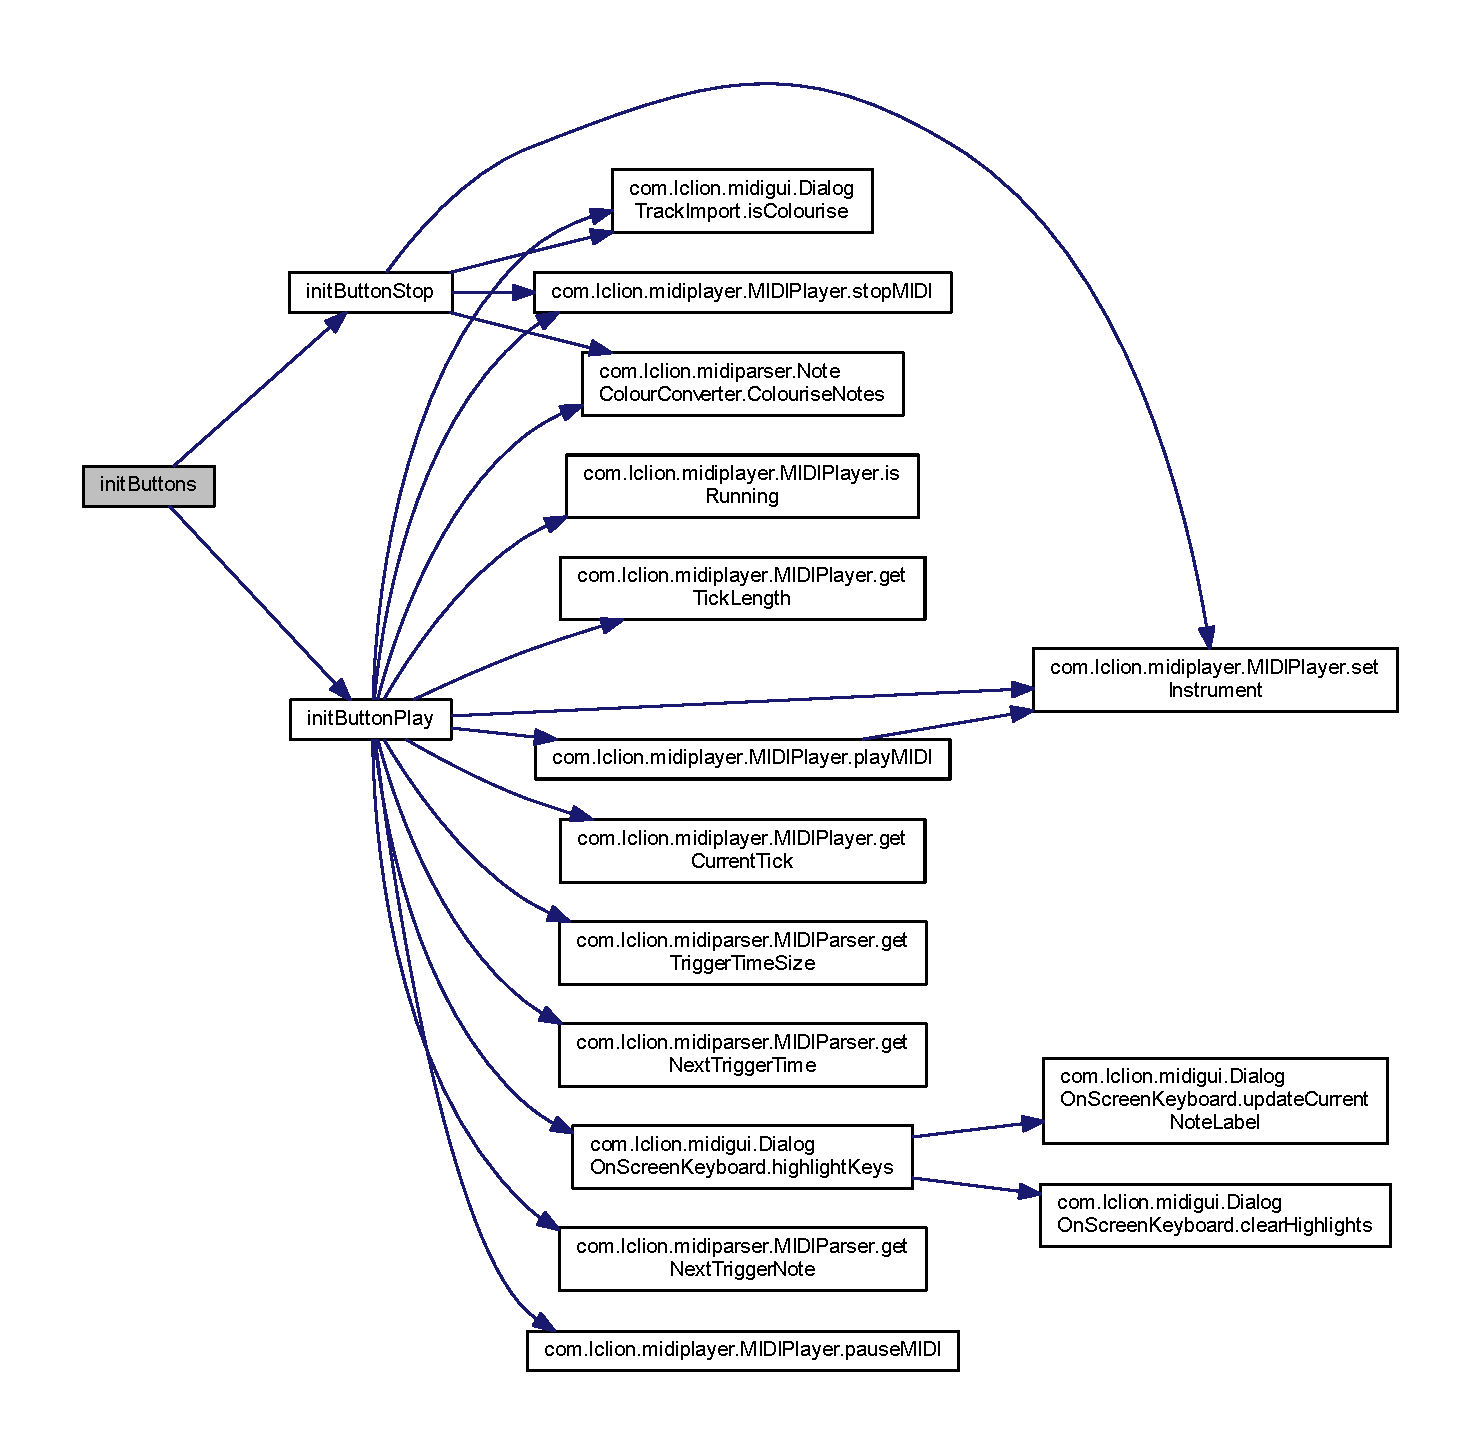
\includegraphics[width=350pt]{classcom_1_1lclion_1_1midigui_1_1_j_frame_m_i_d_i_piano_sheet_creator_a27d3ba5afb772cc36c9a432c28975ace_cgraph}
\end{center}
\end{figure}


\hypertarget{classcom_1_1lclion_1_1midigui_1_1_j_frame_m_i_d_i_piano_sheet_creator_a2f0269651e213406c54a93a303ef9154}{\index{com\+::lclion\+::midigui\+::\+J\+Frame\+M\+I\+D\+I\+Piano\+Sheet\+Creator@{com\+::lclion\+::midigui\+::\+J\+Frame\+M\+I\+D\+I\+Piano\+Sheet\+Creator}!init\+Button\+Stop@{init\+Button\+Stop}}
\index{init\+Button\+Stop@{init\+Button\+Stop}!com\+::lclion\+::midigui\+::\+J\+Frame\+M\+I\+D\+I\+Piano\+Sheet\+Creator@{com\+::lclion\+::midigui\+::\+J\+Frame\+M\+I\+D\+I\+Piano\+Sheet\+Creator}}
\subsubsection[{init\+Button\+Stop}]{\setlength{\rightskip}{0pt plus 5cm}void init\+Button\+Stop (
\begin{DoxyParamCaption}
{}
\end{DoxyParamCaption}
)\hspace{0.3cm}{\ttfamily [private]}}}\label{classcom_1_1lclion_1_1midigui_1_1_j_frame_m_i_d_i_piano_sheet_creator_a2f0269651e213406c54a93a303ef9154}


Initialise the Stop Button and it's event listener. 

Stops the M\+I\+D\+I playback, the autoplay\+Timer and sets G\+U\+I components to the stop state.

\begin{DoxySeeAlso}{See also}
autoplay\+Timers 
\end{DoxySeeAlso}


Here is the call graph for this function\+:\nopagebreak
\begin{figure}[H]
\begin{center}
\leavevmode
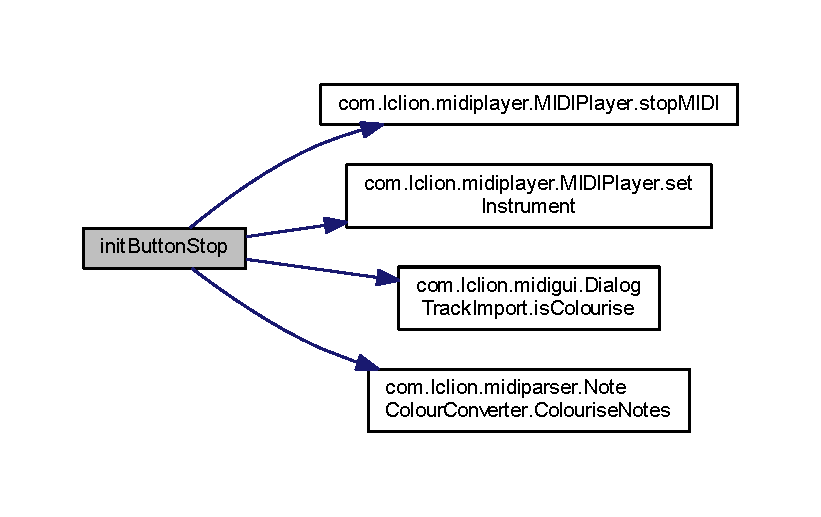
\includegraphics[width=350pt]{classcom_1_1lclion_1_1midigui_1_1_j_frame_m_i_d_i_piano_sheet_creator_a2f0269651e213406c54a93a303ef9154_cgraph}
\end{center}
\end{figure}


\hypertarget{classcom_1_1lclion_1_1midigui_1_1_j_frame_m_i_d_i_piano_sheet_creator_a8512e0e195013a23bdecce9bfb93b04c}{\index{com\+::lclion\+::midigui\+::\+J\+Frame\+M\+I\+D\+I\+Piano\+Sheet\+Creator@{com\+::lclion\+::midigui\+::\+J\+Frame\+M\+I\+D\+I\+Piano\+Sheet\+Creator}!init\+Dialogs@{init\+Dialogs}}
\index{init\+Dialogs@{init\+Dialogs}!com\+::lclion\+::midigui\+::\+J\+Frame\+M\+I\+D\+I\+Piano\+Sheet\+Creator@{com\+::lclion\+::midigui\+::\+J\+Frame\+M\+I\+D\+I\+Piano\+Sheet\+Creator}}
\subsubsection[{init\+Dialogs}]{\setlength{\rightskip}{0pt plus 5cm}void init\+Dialogs (
\begin{DoxyParamCaption}
{}
\end{DoxyParamCaption}
)\hspace{0.3cm}{\ttfamily [private]}}}\label{classcom_1_1lclion_1_1midigui_1_1_j_frame_m_i_d_i_piano_sheet_creator_a8512e0e195013a23bdecce9bfb93b04c}


Initialise dialogs related to this window. 

Also sets G\+U\+I location relative to the main window \hypertarget{classcom_1_1lclion_1_1midigui_1_1_j_frame_m_i_d_i_piano_sheet_creator_a0b0e9cd41d19d9cb52443c381a519994}{\index{com\+::lclion\+::midigui\+::\+J\+Frame\+M\+I\+D\+I\+Piano\+Sheet\+Creator@{com\+::lclion\+::midigui\+::\+J\+Frame\+M\+I\+D\+I\+Piano\+Sheet\+Creator}!init\+Menu\+Bar@{init\+Menu\+Bar}}
\index{init\+Menu\+Bar@{init\+Menu\+Bar}!com\+::lclion\+::midigui\+::\+J\+Frame\+M\+I\+D\+I\+Piano\+Sheet\+Creator@{com\+::lclion\+::midigui\+::\+J\+Frame\+M\+I\+D\+I\+Piano\+Sheet\+Creator}}
\subsubsection[{init\+Menu\+Bar}]{\setlength{\rightskip}{0pt plus 5cm}void init\+Menu\+Bar (
\begin{DoxyParamCaption}
{}
\end{DoxyParamCaption}
)\hspace{0.3cm}{\ttfamily [private]}}}\label{classcom_1_1lclion_1_1midigui_1_1_j_frame_m_i_d_i_piano_sheet_creator_a0b0e9cd41d19d9cb52443c381a519994}


Initialise Menu Bars related to this window. 



Here is the call graph for this function\+:
\nopagebreak
\begin{figure}[H]
\begin{center}
\leavevmode
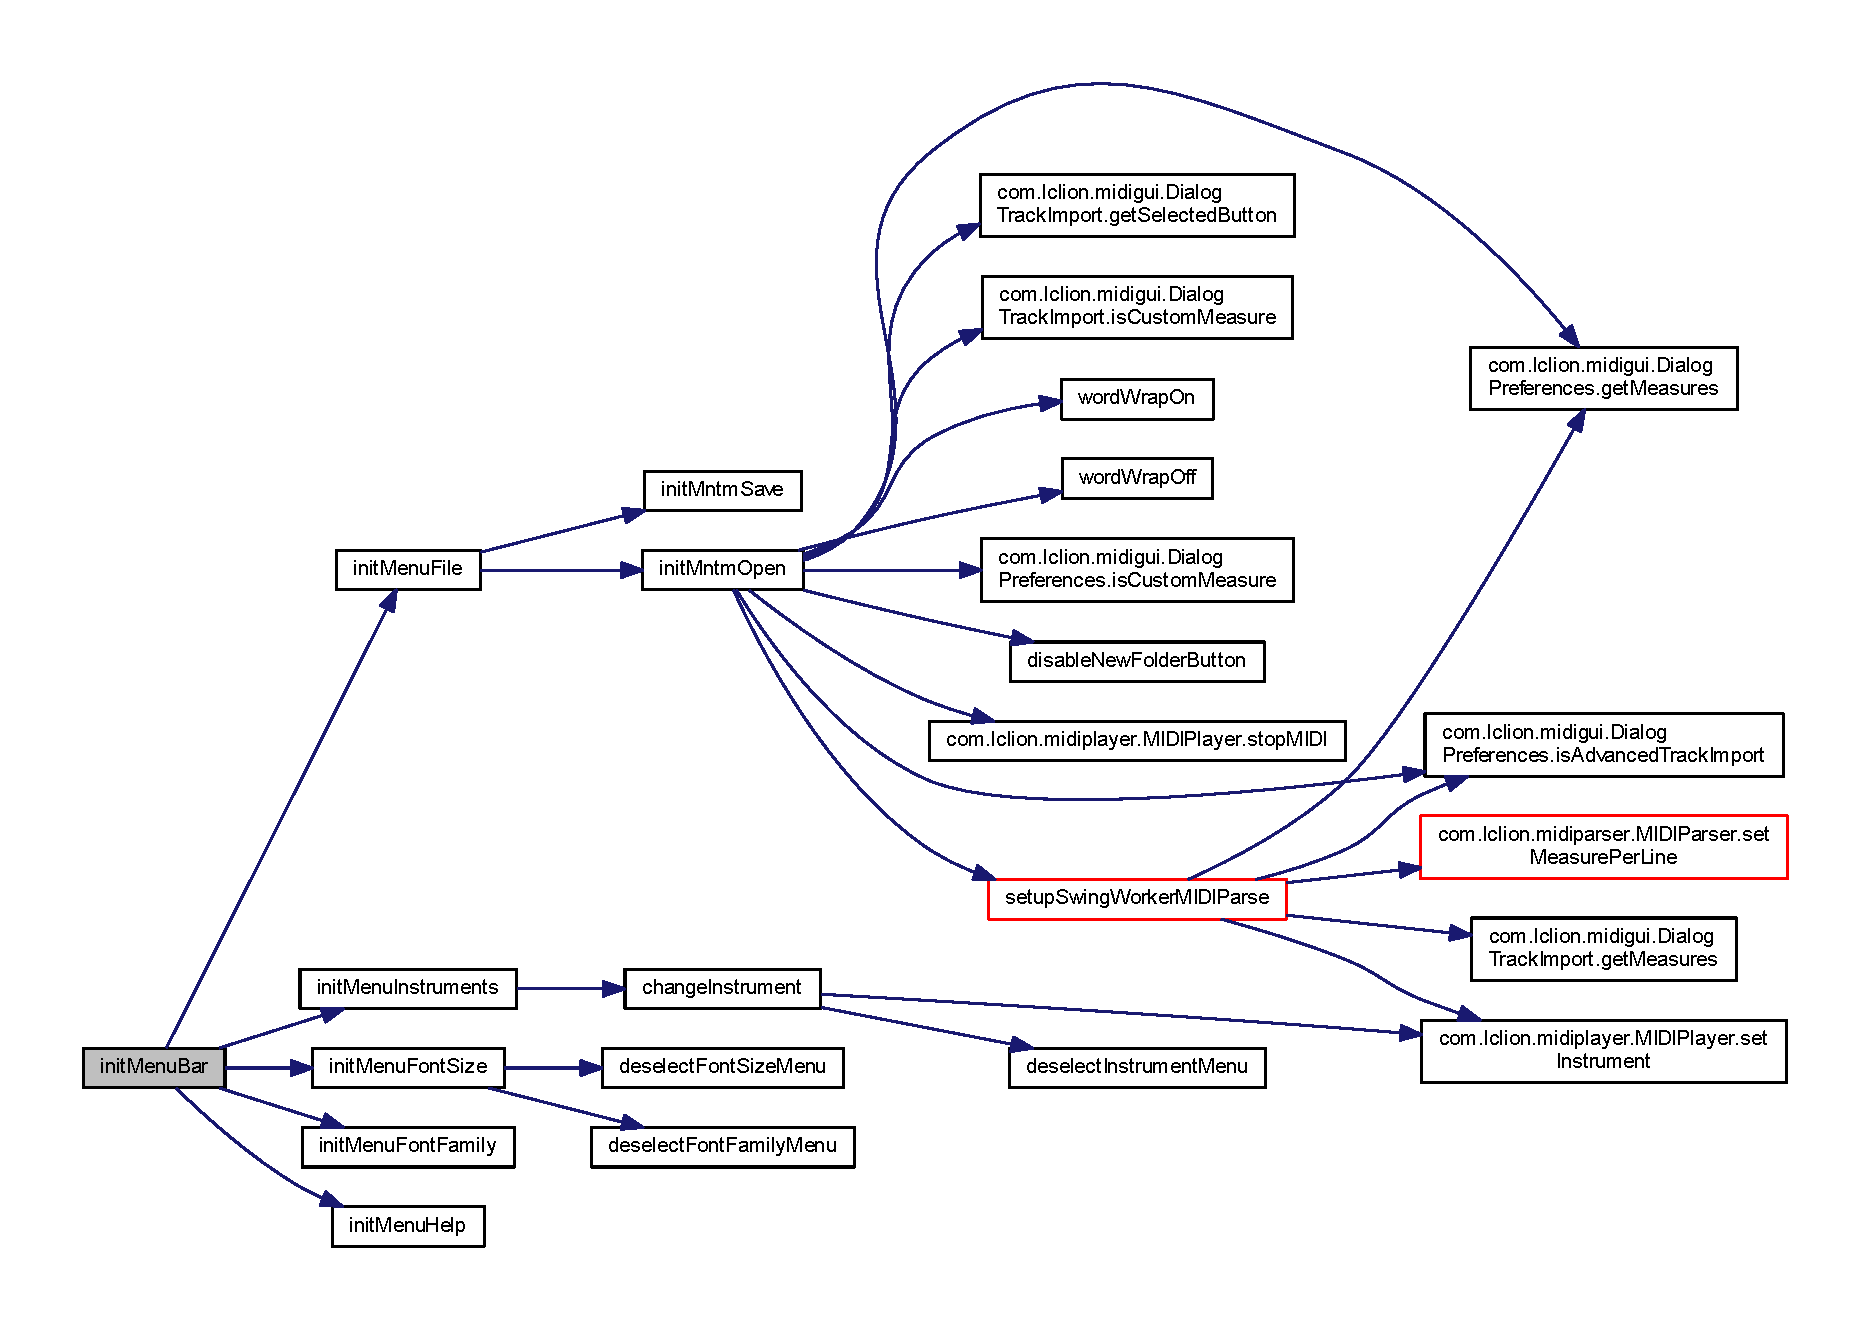
\includegraphics[width=350pt]{classcom_1_1lclion_1_1midigui_1_1_j_frame_m_i_d_i_piano_sheet_creator_a0b0e9cd41d19d9cb52443c381a519994_cgraph}
\end{center}
\end{figure}


\hypertarget{classcom_1_1lclion_1_1midigui_1_1_j_frame_m_i_d_i_piano_sheet_creator_a48db1e242ba2acdb007ab6e8f5c245c6}{\index{com\+::lclion\+::midigui\+::\+J\+Frame\+M\+I\+D\+I\+Piano\+Sheet\+Creator@{com\+::lclion\+::midigui\+::\+J\+Frame\+M\+I\+D\+I\+Piano\+Sheet\+Creator}!init\+Menu\+File@{init\+Menu\+File}}
\index{init\+Menu\+File@{init\+Menu\+File}!com\+::lclion\+::midigui\+::\+J\+Frame\+M\+I\+D\+I\+Piano\+Sheet\+Creator@{com\+::lclion\+::midigui\+::\+J\+Frame\+M\+I\+D\+I\+Piano\+Sheet\+Creator}}
\subsubsection[{init\+Menu\+File}]{\setlength{\rightskip}{0pt plus 5cm}void init\+Menu\+File (
\begin{DoxyParamCaption}
{}
\end{DoxyParamCaption}
)\hspace{0.3cm}{\ttfamily [private]}}}\label{classcom_1_1lclion_1_1midigui_1_1_j_frame_m_i_d_i_piano_sheet_creator_a48db1e242ba2acdb007ab6e8f5c245c6}


Initialise the menus in the main window. 



Here is the call graph for this function\+:
\nopagebreak
\begin{figure}[H]
\begin{center}
\leavevmode
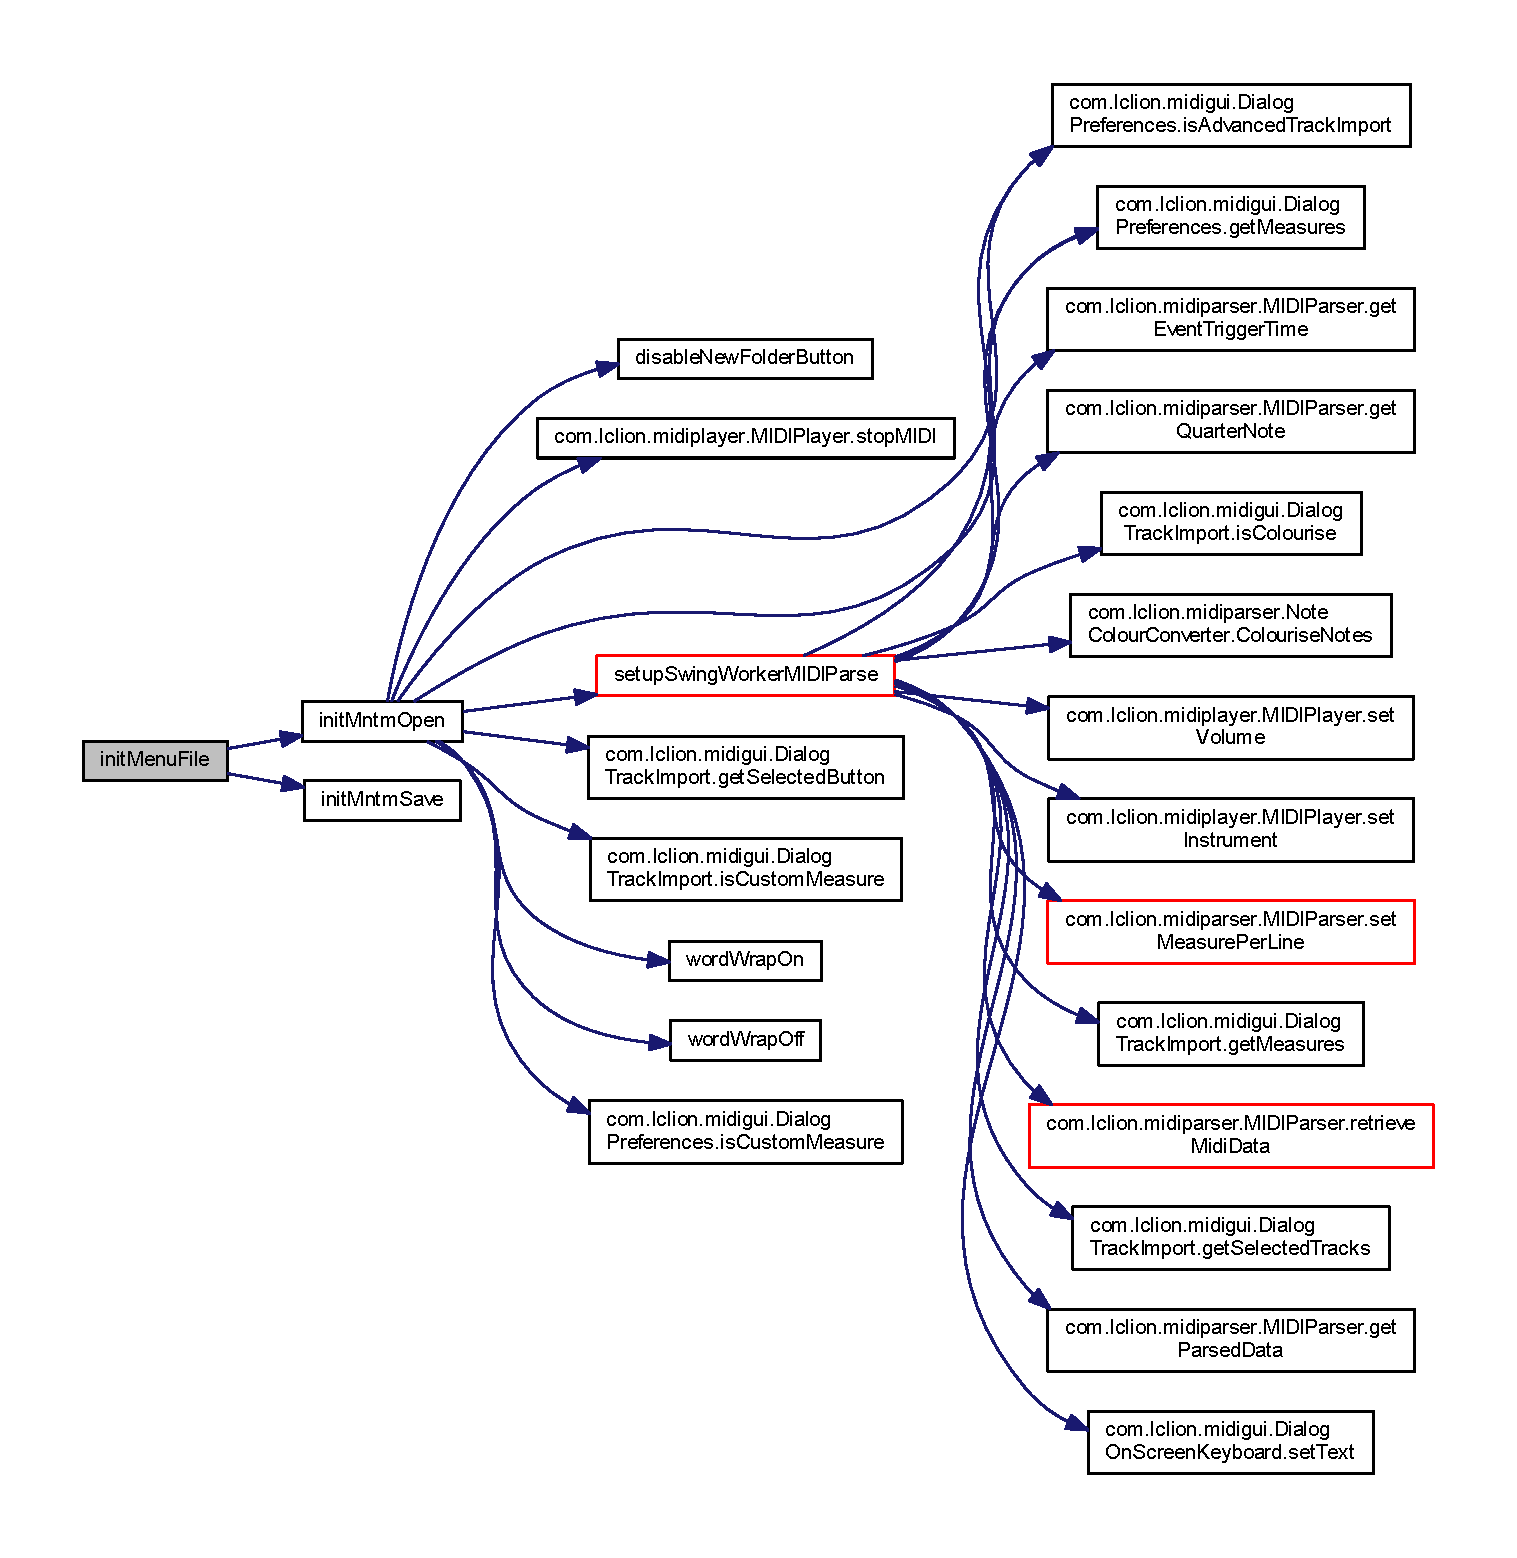
\includegraphics[width=350pt]{classcom_1_1lclion_1_1midigui_1_1_j_frame_m_i_d_i_piano_sheet_creator_a48db1e242ba2acdb007ab6e8f5c245c6_cgraph}
\end{center}
\end{figure}


\hypertarget{classcom_1_1lclion_1_1midigui_1_1_j_frame_m_i_d_i_piano_sheet_creator_a69eddc42278f45218c12c51637b36d34}{\index{com\+::lclion\+::midigui\+::\+J\+Frame\+M\+I\+D\+I\+Piano\+Sheet\+Creator@{com\+::lclion\+::midigui\+::\+J\+Frame\+M\+I\+D\+I\+Piano\+Sheet\+Creator}!init\+Menu\+Font\+Family@{init\+Menu\+Font\+Family}}
\index{init\+Menu\+Font\+Family@{init\+Menu\+Font\+Family}!com\+::lclion\+::midigui\+::\+J\+Frame\+M\+I\+D\+I\+Piano\+Sheet\+Creator@{com\+::lclion\+::midigui\+::\+J\+Frame\+M\+I\+D\+I\+Piano\+Sheet\+Creator}}
\subsubsection[{init\+Menu\+Font\+Family}]{\setlength{\rightskip}{0pt plus 5cm}void init\+Menu\+Font\+Family (
\begin{DoxyParamCaption}
{}
\end{DoxyParamCaption}
)\hspace{0.3cm}{\ttfamily [private]}}}\label{classcom_1_1lclion_1_1midigui_1_1_j_frame_m_i_d_i_piano_sheet_creator_a69eddc42278f45218c12c51637b36d34}
\hypertarget{classcom_1_1lclion_1_1midigui_1_1_j_frame_m_i_d_i_piano_sheet_creator_a508329abe82be4cf7842ca7c468f18c8}{\index{com\+::lclion\+::midigui\+::\+J\+Frame\+M\+I\+D\+I\+Piano\+Sheet\+Creator@{com\+::lclion\+::midigui\+::\+J\+Frame\+M\+I\+D\+I\+Piano\+Sheet\+Creator}!init\+Menu\+Font\+Size@{init\+Menu\+Font\+Size}}
\index{init\+Menu\+Font\+Size@{init\+Menu\+Font\+Size}!com\+::lclion\+::midigui\+::\+J\+Frame\+M\+I\+D\+I\+Piano\+Sheet\+Creator@{com\+::lclion\+::midigui\+::\+J\+Frame\+M\+I\+D\+I\+Piano\+Sheet\+Creator}}
\subsubsection[{init\+Menu\+Font\+Size}]{\setlength{\rightskip}{0pt plus 5cm}void init\+Menu\+Font\+Size (
\begin{DoxyParamCaption}
{}
\end{DoxyParamCaption}
)\hspace{0.3cm}{\ttfamily [private]}}}\label{classcom_1_1lclion_1_1midigui_1_1_j_frame_m_i_d_i_piano_sheet_creator_a508329abe82be4cf7842ca7c468f18c8}


Here is the call graph for this function\+:\nopagebreak
\begin{figure}[H]
\begin{center}
\leavevmode
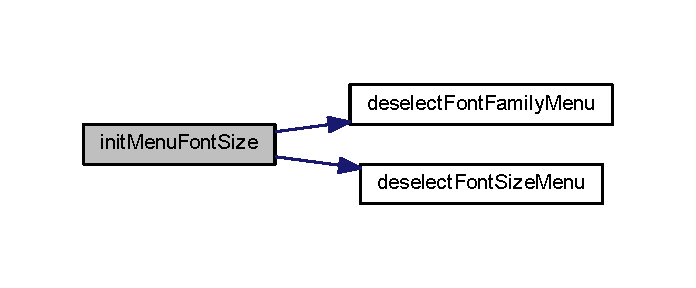
\includegraphics[width=334pt]{classcom_1_1lclion_1_1midigui_1_1_j_frame_m_i_d_i_piano_sheet_creator_a508329abe82be4cf7842ca7c468f18c8_cgraph}
\end{center}
\end{figure}


\hypertarget{classcom_1_1lclion_1_1midigui_1_1_j_frame_m_i_d_i_piano_sheet_creator_a098b454223f052d378bd20af06f6ddf0}{\index{com\+::lclion\+::midigui\+::\+J\+Frame\+M\+I\+D\+I\+Piano\+Sheet\+Creator@{com\+::lclion\+::midigui\+::\+J\+Frame\+M\+I\+D\+I\+Piano\+Sheet\+Creator}!init\+Menu\+Help@{init\+Menu\+Help}}
\index{init\+Menu\+Help@{init\+Menu\+Help}!com\+::lclion\+::midigui\+::\+J\+Frame\+M\+I\+D\+I\+Piano\+Sheet\+Creator@{com\+::lclion\+::midigui\+::\+J\+Frame\+M\+I\+D\+I\+Piano\+Sheet\+Creator}}
\subsubsection[{init\+Menu\+Help}]{\setlength{\rightskip}{0pt plus 5cm}void init\+Menu\+Help (
\begin{DoxyParamCaption}
{}
\end{DoxyParamCaption}
)\hspace{0.3cm}{\ttfamily [private]}}}\label{classcom_1_1lclion_1_1midigui_1_1_j_frame_m_i_d_i_piano_sheet_creator_a098b454223f052d378bd20af06f6ddf0}


Initialise Menu Help related to this window. 

\hypertarget{classcom_1_1lclion_1_1midigui_1_1_j_frame_m_i_d_i_piano_sheet_creator_a200519724ded34307a2e8c0cd6497a56}{\index{com\+::lclion\+::midigui\+::\+J\+Frame\+M\+I\+D\+I\+Piano\+Sheet\+Creator@{com\+::lclion\+::midigui\+::\+J\+Frame\+M\+I\+D\+I\+Piano\+Sheet\+Creator}!init\+Menu\+Instruments@{init\+Menu\+Instruments}}
\index{init\+Menu\+Instruments@{init\+Menu\+Instruments}!com\+::lclion\+::midigui\+::\+J\+Frame\+M\+I\+D\+I\+Piano\+Sheet\+Creator@{com\+::lclion\+::midigui\+::\+J\+Frame\+M\+I\+D\+I\+Piano\+Sheet\+Creator}}
\subsubsection[{init\+Menu\+Instruments}]{\setlength{\rightskip}{0pt plus 5cm}void init\+Menu\+Instruments (
\begin{DoxyParamCaption}
{}
\end{DoxyParamCaption}
)\hspace{0.3cm}{\ttfamily [private]}}}\label{classcom_1_1lclion_1_1midigui_1_1_j_frame_m_i_d_i_piano_sheet_creator_a200519724ded34307a2e8c0cd6497a56}


Here is the call graph for this function\+:\nopagebreak
\begin{figure}[H]
\begin{center}
\leavevmode
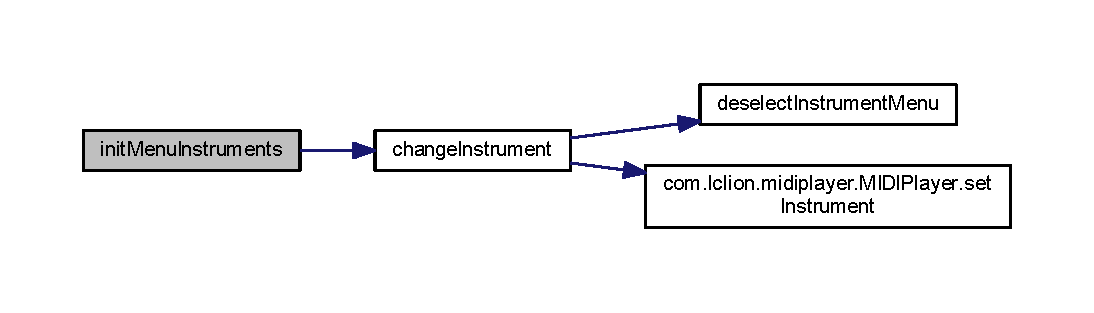
\includegraphics[width=350pt]{classcom_1_1lclion_1_1midigui_1_1_j_frame_m_i_d_i_piano_sheet_creator_a200519724ded34307a2e8c0cd6497a56_cgraph}
\end{center}
\end{figure}


\hypertarget{classcom_1_1lclion_1_1midigui_1_1_j_frame_m_i_d_i_piano_sheet_creator_a6de8f8799e0b919151dd7d602565c867}{\index{com\+::lclion\+::midigui\+::\+J\+Frame\+M\+I\+D\+I\+Piano\+Sheet\+Creator@{com\+::lclion\+::midigui\+::\+J\+Frame\+M\+I\+D\+I\+Piano\+Sheet\+Creator}!init\+Mntm\+Open@{init\+Mntm\+Open}}
\index{init\+Mntm\+Open@{init\+Mntm\+Open}!com\+::lclion\+::midigui\+::\+J\+Frame\+M\+I\+D\+I\+Piano\+Sheet\+Creator@{com\+::lclion\+::midigui\+::\+J\+Frame\+M\+I\+D\+I\+Piano\+Sheet\+Creator}}
\subsubsection[{init\+Mntm\+Open}]{\setlength{\rightskip}{0pt plus 5cm}void init\+Mntm\+Open (
\begin{DoxyParamCaption}
{}
\end{DoxyParamCaption}
)\hspace{0.3cm}{\ttfamily [private]}}}\label{classcom_1_1lclion_1_1midigui_1_1_j_frame_m_i_d_i_piano_sheet_creator_a6de8f8799e0b919151dd7d602565c867}


Menu to open a M\+I\+D\+I File. 

Opens M\+I\+D\+I File by calling a file chooser, and setting up necessary options for it using Dialog Import Options.

Also sets up an Event listener and a Swing\+Worker when parsing M\+I\+D\+I File

\begin{DoxySeeAlso}{See also}
\hyperlink{classcom_1_1lclion_1_1midigui_1_1_dialog_track_import}{Dialog\+Track\+Import} 
\end{DoxySeeAlso}


Here is the call graph for this function\+:
\nopagebreak
\begin{figure}[H]
\begin{center}
\leavevmode
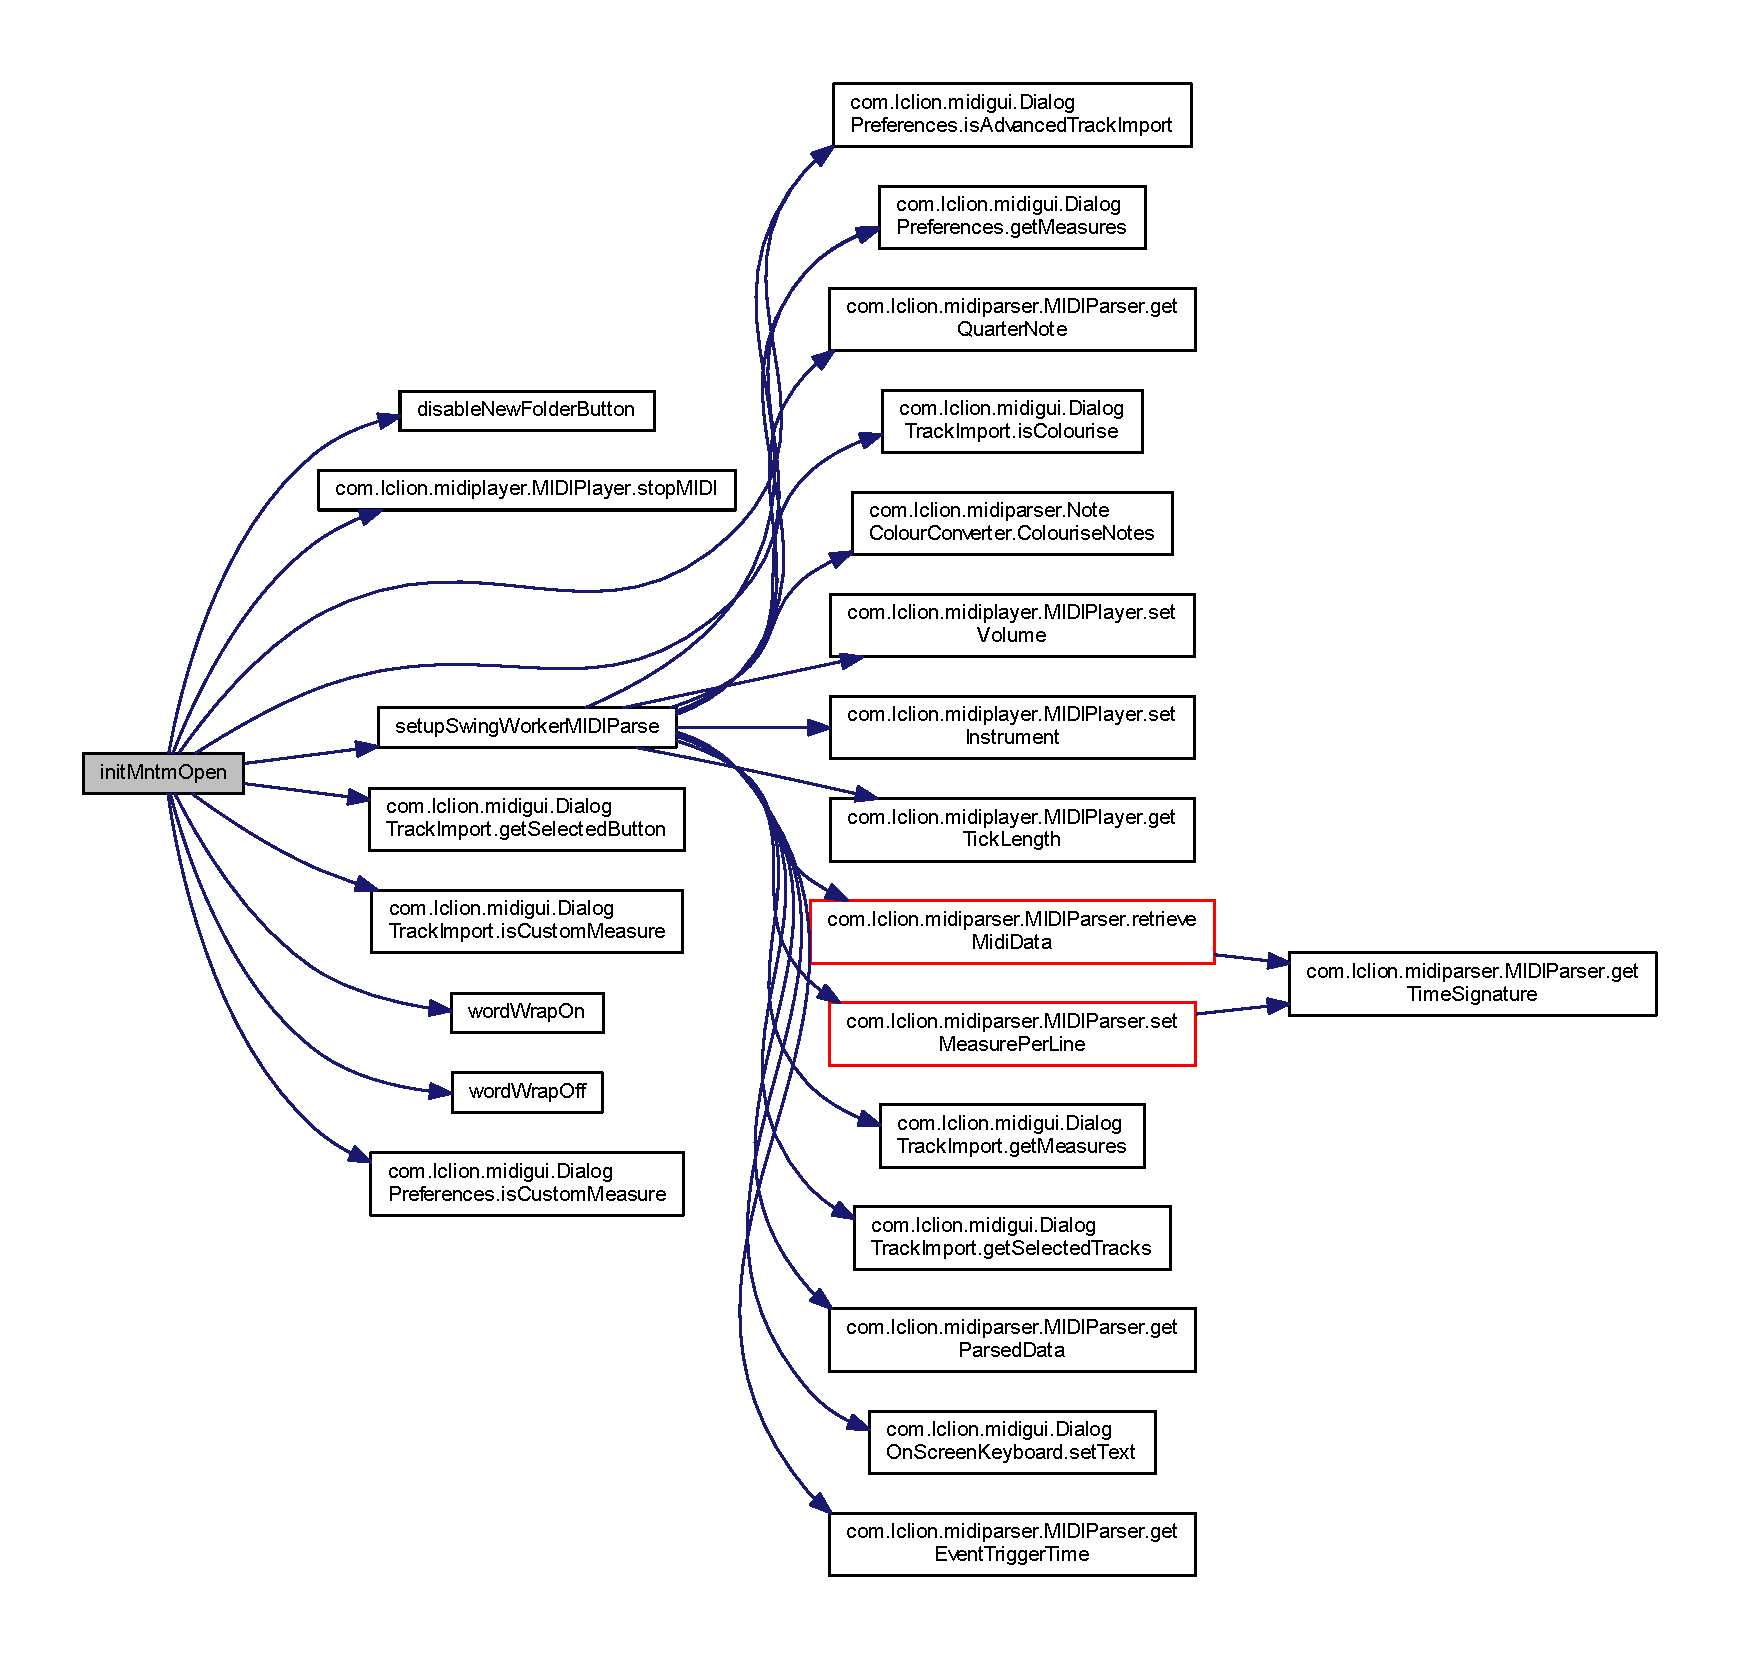
\includegraphics[width=350pt]{classcom_1_1lclion_1_1midigui_1_1_j_frame_m_i_d_i_piano_sheet_creator_a6de8f8799e0b919151dd7d602565c867_cgraph}
\end{center}
\end{figure}


\hypertarget{classcom_1_1lclion_1_1midigui_1_1_j_frame_m_i_d_i_piano_sheet_creator_a2b96b6ece7e72836a6e472f85951e297}{\index{com\+::lclion\+::midigui\+::\+J\+Frame\+M\+I\+D\+I\+Piano\+Sheet\+Creator@{com\+::lclion\+::midigui\+::\+J\+Frame\+M\+I\+D\+I\+Piano\+Sheet\+Creator}!init\+Mntm\+Save@{init\+Mntm\+Save}}
\index{init\+Mntm\+Save@{init\+Mntm\+Save}!com\+::lclion\+::midigui\+::\+J\+Frame\+M\+I\+D\+I\+Piano\+Sheet\+Creator@{com\+::lclion\+::midigui\+::\+J\+Frame\+M\+I\+D\+I\+Piano\+Sheet\+Creator}}
\subsubsection[{init\+Mntm\+Save}]{\setlength{\rightskip}{0pt plus 5cm}void init\+Mntm\+Save (
\begin{DoxyParamCaption}
{}
\end{DoxyParamCaption}
)\hspace{0.3cm}{\ttfamily [private]}}}\label{classcom_1_1lclion_1_1midigui_1_1_j_frame_m_i_d_i_piano_sheet_creator_a2b96b6ece7e72836a6e472f85951e297}


Menu to save the parsed piano sheet to text file (notepad's .txt file format) 

\hypertarget{classcom_1_1lclion_1_1midigui_1_1_j_frame_m_i_d_i_piano_sheet_creator_a64517851bfe923ade6f59648b3a9f4e3}{\index{com\+::lclion\+::midigui\+::\+J\+Frame\+M\+I\+D\+I\+Piano\+Sheet\+Creator@{com\+::lclion\+::midigui\+::\+J\+Frame\+M\+I\+D\+I\+Piano\+Sheet\+Creator}!init\+Progress\+Sliders@{init\+Progress\+Sliders}}
\index{init\+Progress\+Sliders@{init\+Progress\+Sliders}!com\+::lclion\+::midigui\+::\+J\+Frame\+M\+I\+D\+I\+Piano\+Sheet\+Creator@{com\+::lclion\+::midigui\+::\+J\+Frame\+M\+I\+D\+I\+Piano\+Sheet\+Creator}}
\subsubsection[{init\+Progress\+Sliders}]{\setlength{\rightskip}{0pt plus 5cm}void init\+Progress\+Sliders (
\begin{DoxyParamCaption}
{}
\end{DoxyParamCaption}
)\hspace{0.3cm}{\ttfamily [private]}}}\label{classcom_1_1lclion_1_1midigui_1_1_j_frame_m_i_d_i_piano_sheet_creator_a64517851bfe923ade6f59648b3a9f4e3}


Initialise sliders related to this window. 



Here is the call graph for this function\+:\nopagebreak
\begin{figure}[H]
\begin{center}
\leavevmode
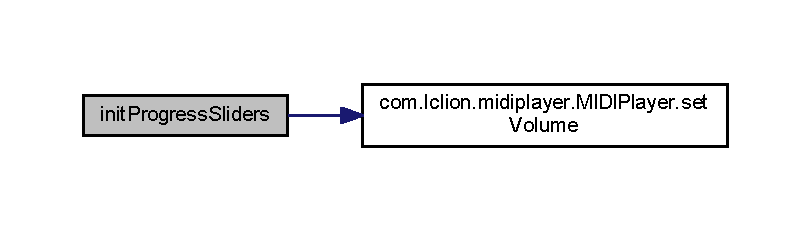
\includegraphics[width=350pt]{classcom_1_1lclion_1_1midigui_1_1_j_frame_m_i_d_i_piano_sheet_creator_a64517851bfe923ade6f59648b3a9f4e3_cgraph}
\end{center}
\end{figure}


\hypertarget{classcom_1_1lclion_1_1midigui_1_1_j_frame_m_i_d_i_piano_sheet_creator_af5b3b9751934a25e7d0b73cf458cea99}{\index{com\+::lclion\+::midigui\+::\+J\+Frame\+M\+I\+D\+I\+Piano\+Sheet\+Creator@{com\+::lclion\+::midigui\+::\+J\+Frame\+M\+I\+D\+I\+Piano\+Sheet\+Creator}!init\+Text\+Pane@{init\+Text\+Pane}}
\index{init\+Text\+Pane@{init\+Text\+Pane}!com\+::lclion\+::midigui\+::\+J\+Frame\+M\+I\+D\+I\+Piano\+Sheet\+Creator@{com\+::lclion\+::midigui\+::\+J\+Frame\+M\+I\+D\+I\+Piano\+Sheet\+Creator}}
\subsubsection[{init\+Text\+Pane}]{\setlength{\rightskip}{0pt plus 5cm}void init\+Text\+Pane (
\begin{DoxyParamCaption}
{}
\end{DoxyParamCaption}
)\hspace{0.3cm}{\ttfamily [private]}}}\label{classcom_1_1lclion_1_1midigui_1_1_j_frame_m_i_d_i_piano_sheet_creator_af5b3b9751934a25e7d0b73cf458cea99}


Initialise text panes related to this window. 



Here is the call graph for this function\+:\nopagebreak
\begin{figure}[H]
\begin{center}
\leavevmode
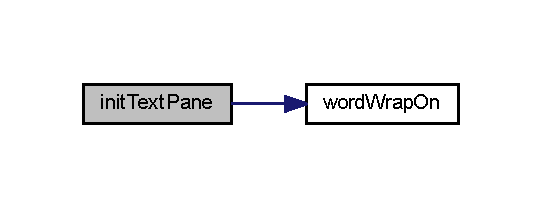
\includegraphics[width=260pt]{classcom_1_1lclion_1_1midigui_1_1_j_frame_m_i_d_i_piano_sheet_creator_af5b3b9751934a25e7d0b73cf458cea99_cgraph}
\end{center}
\end{figure}


\hypertarget{classcom_1_1lclion_1_1midigui_1_1_j_frame_m_i_d_i_piano_sheet_creator_aae03cd254fec1d9f47948ce62a294baf}{\index{com\+::lclion\+::midigui\+::\+J\+Frame\+M\+I\+D\+I\+Piano\+Sheet\+Creator@{com\+::lclion\+::midigui\+::\+J\+Frame\+M\+I\+D\+I\+Piano\+Sheet\+Creator}!setup\+Swing\+Worker\+M\+I\+D\+I\+Parse@{setup\+Swing\+Worker\+M\+I\+D\+I\+Parse}}
\index{setup\+Swing\+Worker\+M\+I\+D\+I\+Parse@{setup\+Swing\+Worker\+M\+I\+D\+I\+Parse}!com\+::lclion\+::midigui\+::\+J\+Frame\+M\+I\+D\+I\+Piano\+Sheet\+Creator@{com\+::lclion\+::midigui\+::\+J\+Frame\+M\+I\+D\+I\+Piano\+Sheet\+Creator}}
\subsubsection[{setup\+Swing\+Worker\+M\+I\+D\+I\+Parse}]{\setlength{\rightskip}{0pt plus 5cm}Swing\+Worker$<$String, Void$>$ setup\+Swing\+Worker\+M\+I\+D\+I\+Parse (
\begin{DoxyParamCaption}
\item[{final File}]{file}
\end{DoxyParamCaption}
)\hspace{0.3cm}{\ttfamily [private]}}}\label{classcom_1_1lclion_1_1midigui_1_1_j_frame_m_i_d_i_piano_sheet_creator_aae03cd254fec1d9f47948ce62a294baf}


Returns the Swing\+Worker required to handle M\+I\+D\+I Parsing (Swing\+Worker prevents G\+U\+I freezing) 


\begin{DoxyParams}{Parameters}
{\em file} & The M\+I\+D\+I file to parse \\
\hline
\end{DoxyParams}
\begin{DoxyReturn}{Returns}
Swing\+Worker The Swing\+Worker that handles the actual midi\+Parsing operations 
\end{DoxyReturn}


Here is the call graph for this function\+:
\nopagebreak
\begin{figure}[H]
\begin{center}
\leavevmode
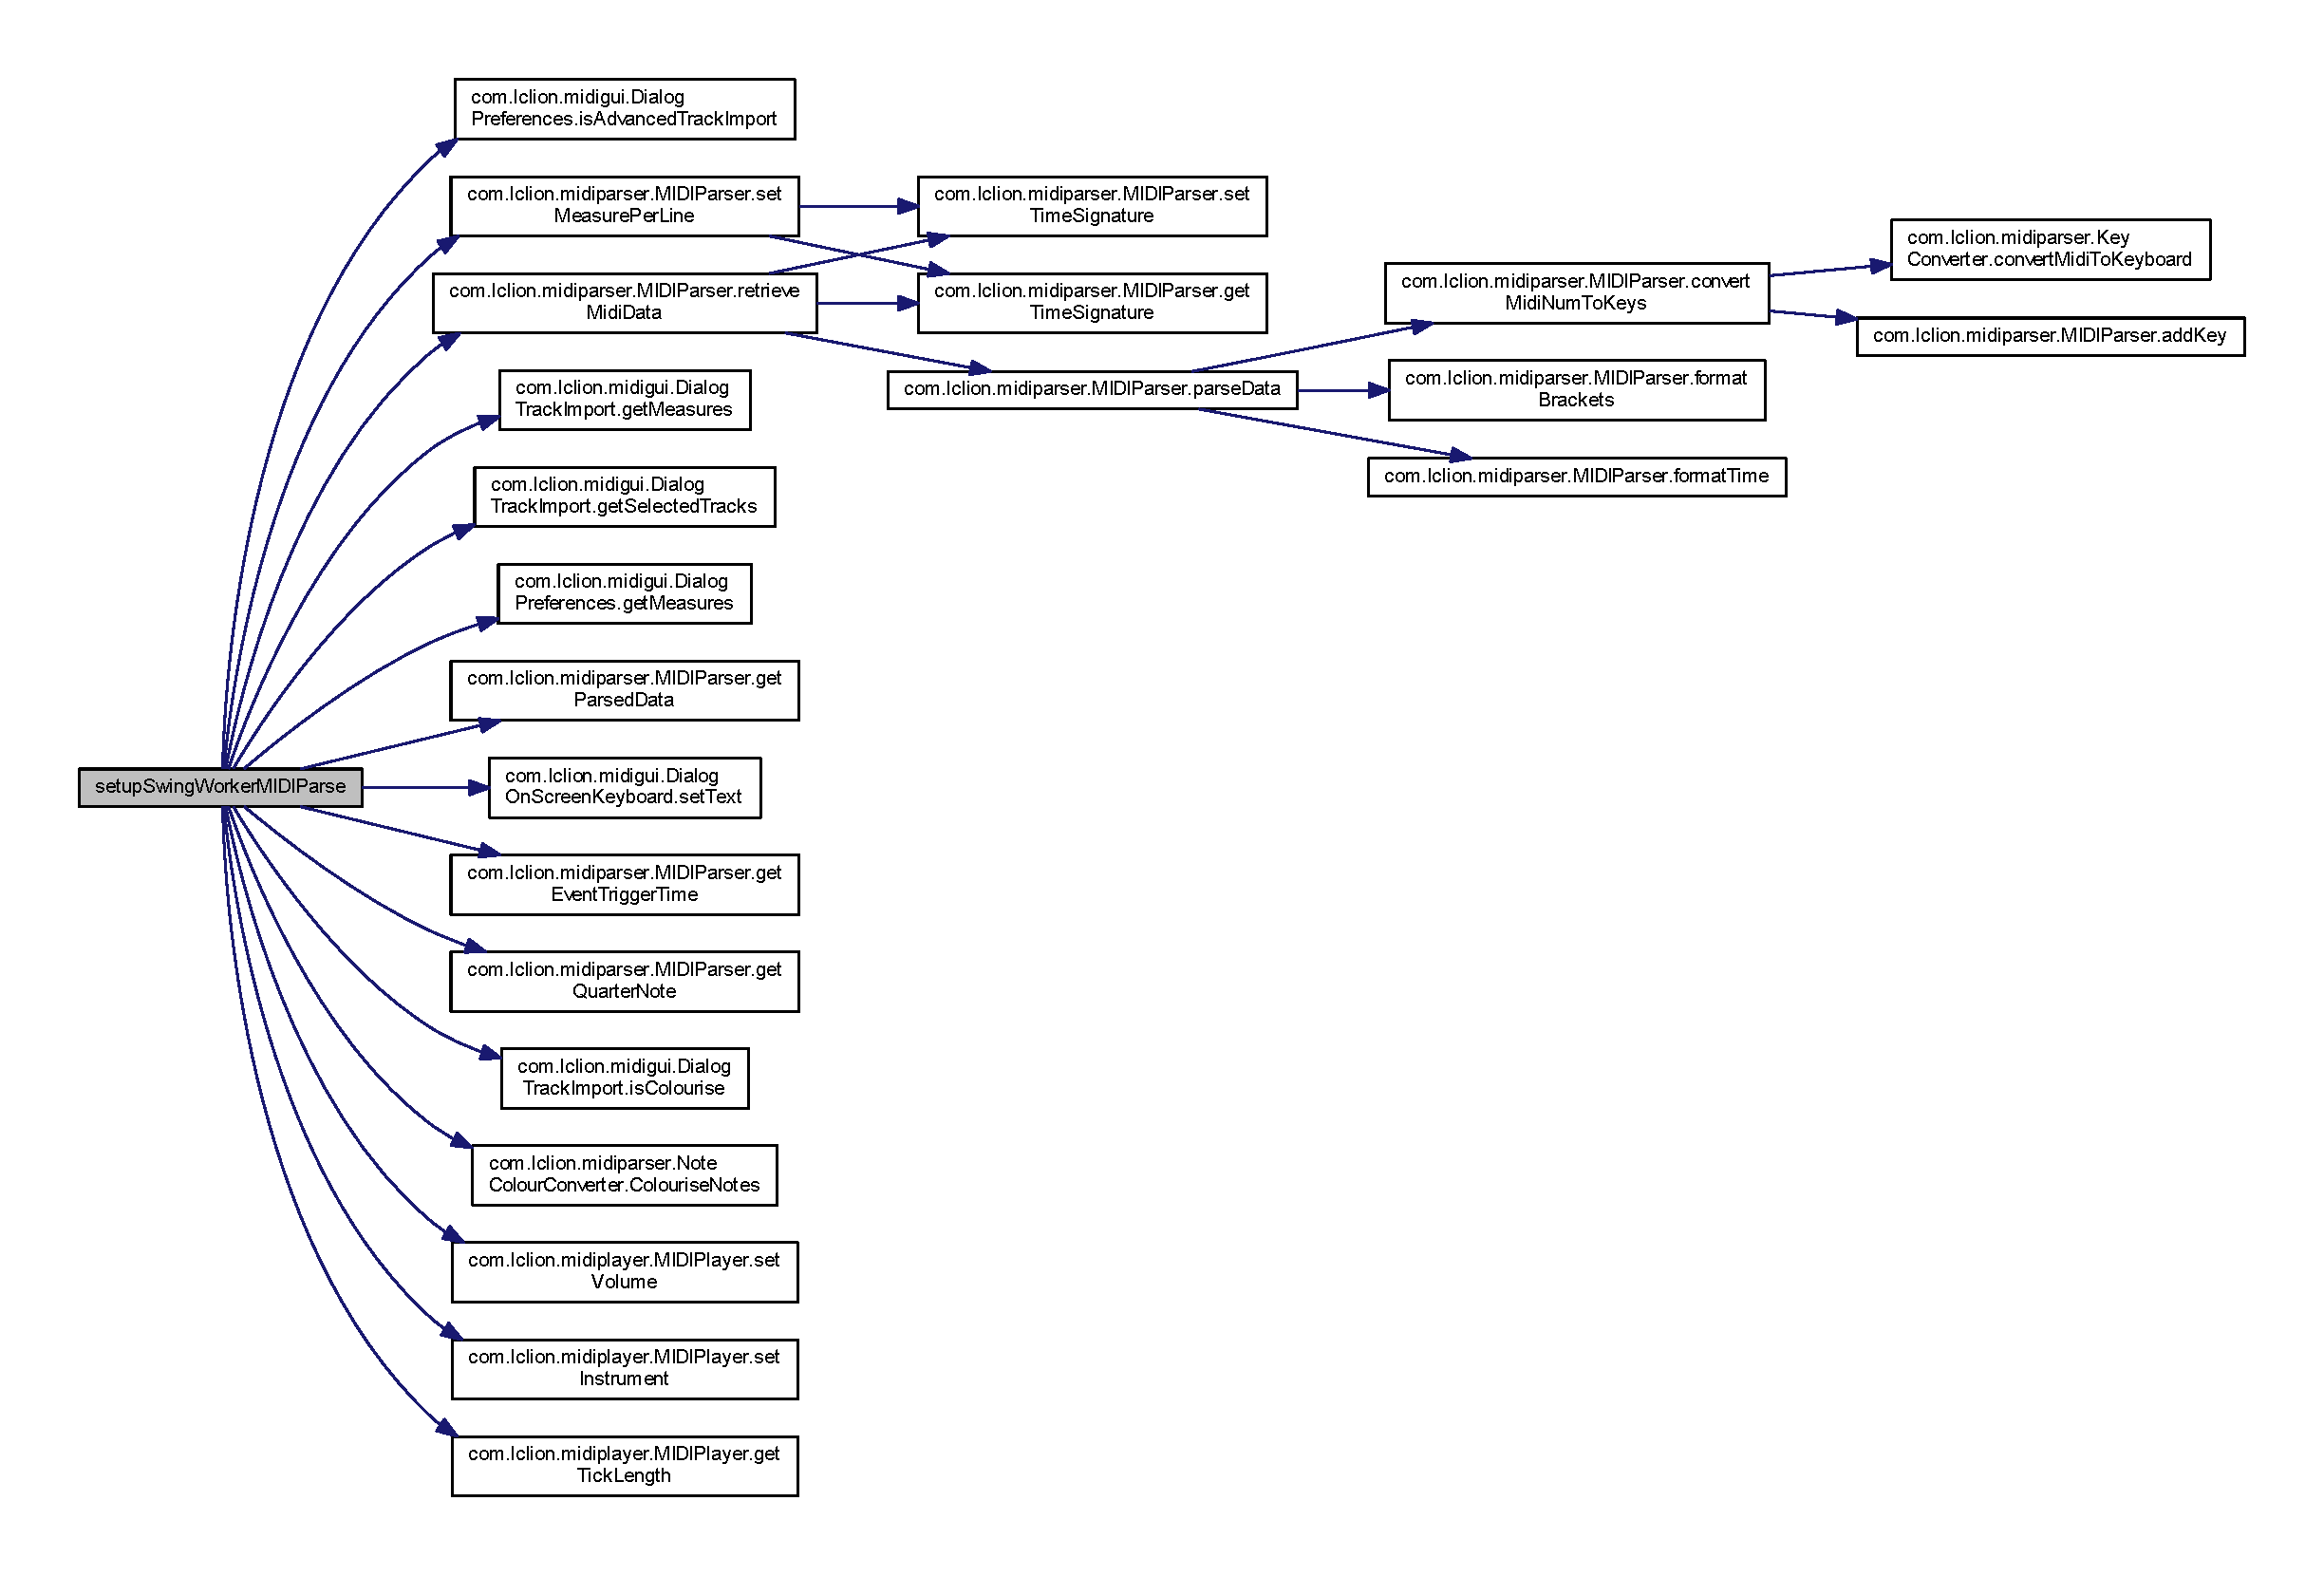
\includegraphics[width=350pt]{classcom_1_1lclion_1_1midigui_1_1_j_frame_m_i_d_i_piano_sheet_creator_aae03cd254fec1d9f47948ce62a294baf_cgraph}
\end{center}
\end{figure}


\hypertarget{classcom_1_1lclion_1_1midigui_1_1_j_frame_m_i_d_i_piano_sheet_creator_a42f3eed8a1306302bdebd9dea75883c5}{\index{com\+::lclion\+::midigui\+::\+J\+Frame\+M\+I\+D\+I\+Piano\+Sheet\+Creator@{com\+::lclion\+::midigui\+::\+J\+Frame\+M\+I\+D\+I\+Piano\+Sheet\+Creator}!word\+Wrap\+Off@{word\+Wrap\+Off}}
\index{word\+Wrap\+Off@{word\+Wrap\+Off}!com\+::lclion\+::midigui\+::\+J\+Frame\+M\+I\+D\+I\+Piano\+Sheet\+Creator@{com\+::lclion\+::midigui\+::\+J\+Frame\+M\+I\+D\+I\+Piano\+Sheet\+Creator}}
\subsubsection[{word\+Wrap\+Off}]{\setlength{\rightskip}{0pt plus 5cm}void word\+Wrap\+Off (
\begin{DoxyParamCaption}
{}
\end{DoxyParamCaption}
)\hspace{0.3cm}{\ttfamily [private]}}}\label{classcom_1_1lclion_1_1midigui_1_1_j_frame_m_i_d_i_piano_sheet_creator_a42f3eed8a1306302bdebd9dea75883c5}


Wordwrap Off for text panes related to this window. 

\hypertarget{classcom_1_1lclion_1_1midigui_1_1_j_frame_m_i_d_i_piano_sheet_creator_ab462219e37674c0df3744f7de1c980ca}{\index{com\+::lclion\+::midigui\+::\+J\+Frame\+M\+I\+D\+I\+Piano\+Sheet\+Creator@{com\+::lclion\+::midigui\+::\+J\+Frame\+M\+I\+D\+I\+Piano\+Sheet\+Creator}!word\+Wrap\+On@{word\+Wrap\+On}}
\index{word\+Wrap\+On@{word\+Wrap\+On}!com\+::lclion\+::midigui\+::\+J\+Frame\+M\+I\+D\+I\+Piano\+Sheet\+Creator@{com\+::lclion\+::midigui\+::\+J\+Frame\+M\+I\+D\+I\+Piano\+Sheet\+Creator}}
\subsubsection[{word\+Wrap\+On}]{\setlength{\rightskip}{0pt plus 5cm}void word\+Wrap\+On (
\begin{DoxyParamCaption}
{}
\end{DoxyParamCaption}
)\hspace{0.3cm}{\ttfamily [private]}}}\label{classcom_1_1lclion_1_1midigui_1_1_j_frame_m_i_d_i_piano_sheet_creator_ab462219e37674c0df3744f7de1c980ca}


Wordwrap On for text panes related to this window. 



\subsection{Member Data Documentation}
\hypertarget{classcom_1_1lclion_1_1midigui_1_1_j_frame_m_i_d_i_piano_sheet_creator_a172d0561900ff10f21cbf9562fa3c261}{\index{com\+::lclion\+::midigui\+::\+J\+Frame\+M\+I\+D\+I\+Piano\+Sheet\+Creator@{com\+::lclion\+::midigui\+::\+J\+Frame\+M\+I\+D\+I\+Piano\+Sheet\+Creator}!autoplay\+Timer@{autoplay\+Timer}}
\index{autoplay\+Timer@{autoplay\+Timer}!com\+::lclion\+::midigui\+::\+J\+Frame\+M\+I\+D\+I\+Piano\+Sheet\+Creator@{com\+::lclion\+::midigui\+::\+J\+Frame\+M\+I\+D\+I\+Piano\+Sheet\+Creator}}
\subsubsection[{autoplay\+Timer}]{\setlength{\rightskip}{0pt plus 5cm}Timer autoplay\+Timer = null\hspace{0.3cm}{\ttfamily [private]}}}\label{classcom_1_1lclion_1_1midigui_1_1_j_frame_m_i_d_i_piano_sheet_creator_a172d0561900ff10f21cbf9562fa3c261}
\hypertarget{classcom_1_1lclion_1_1midigui_1_1_j_frame_m_i_d_i_piano_sheet_creator_aa1718d1d474c9cc2c8f72edef9c6d767}{\index{com\+::lclion\+::midigui\+::\+J\+Frame\+M\+I\+D\+I\+Piano\+Sheet\+Creator@{com\+::lclion\+::midigui\+::\+J\+Frame\+M\+I\+D\+I\+Piano\+Sheet\+Creator}!btn\+Play@{btn\+Play}}
\index{btn\+Play@{btn\+Play}!com\+::lclion\+::midigui\+::\+J\+Frame\+M\+I\+D\+I\+Piano\+Sheet\+Creator@{com\+::lclion\+::midigui\+::\+J\+Frame\+M\+I\+D\+I\+Piano\+Sheet\+Creator}}
\subsubsection[{btn\+Play}]{\setlength{\rightskip}{0pt plus 5cm}J\+Button btn\+Play\hspace{0.3cm}{\ttfamily [private]}}}\label{classcom_1_1lclion_1_1midigui_1_1_j_frame_m_i_d_i_piano_sheet_creator_aa1718d1d474c9cc2c8f72edef9c6d767}
\hypertarget{classcom_1_1lclion_1_1midigui_1_1_j_frame_m_i_d_i_piano_sheet_creator_a3e498460ccccf41b258ee18a8ea8d988}{\index{com\+::lclion\+::midigui\+::\+J\+Frame\+M\+I\+D\+I\+Piano\+Sheet\+Creator@{com\+::lclion\+::midigui\+::\+J\+Frame\+M\+I\+D\+I\+Piano\+Sheet\+Creator}!btn\+Stop@{btn\+Stop}}
\index{btn\+Stop@{btn\+Stop}!com\+::lclion\+::midigui\+::\+J\+Frame\+M\+I\+D\+I\+Piano\+Sheet\+Creator@{com\+::lclion\+::midigui\+::\+J\+Frame\+M\+I\+D\+I\+Piano\+Sheet\+Creator}}
\subsubsection[{btn\+Stop}]{\setlength{\rightskip}{0pt plus 5cm}J\+Button btn\+Stop\hspace{0.3cm}{\ttfamily [private]}}}\label{classcom_1_1lclion_1_1midigui_1_1_j_frame_m_i_d_i_piano_sheet_creator_a3e498460ccccf41b258ee18a8ea8d988}
\hypertarget{classcom_1_1lclion_1_1midigui_1_1_j_frame_m_i_d_i_piano_sheet_creator_acf27febb9f46a2cb5b78ecb7e283e243}{\index{com\+::lclion\+::midigui\+::\+J\+Frame\+M\+I\+D\+I\+Piano\+Sheet\+Creator@{com\+::lclion\+::midigui\+::\+J\+Frame\+M\+I\+D\+I\+Piano\+Sheet\+Creator}!chckbxmntm\+Acoustic\+Grand\+Piano@{chckbxmntm\+Acoustic\+Grand\+Piano}}
\index{chckbxmntm\+Acoustic\+Grand\+Piano@{chckbxmntm\+Acoustic\+Grand\+Piano}!com\+::lclion\+::midigui\+::\+J\+Frame\+M\+I\+D\+I\+Piano\+Sheet\+Creator@{com\+::lclion\+::midigui\+::\+J\+Frame\+M\+I\+D\+I\+Piano\+Sheet\+Creator}}
\subsubsection[{chckbxmntm\+Acoustic\+Grand\+Piano}]{\setlength{\rightskip}{0pt plus 5cm}J\+Check\+Box\+Menu\+Item chckbxmntm\+Acoustic\+Grand\+Piano\hspace{0.3cm}{\ttfamily [private]}}}\label{classcom_1_1lclion_1_1midigui_1_1_j_frame_m_i_d_i_piano_sheet_creator_acf27febb9f46a2cb5b78ecb7e283e243}
\hypertarget{classcom_1_1lclion_1_1midigui_1_1_j_frame_m_i_d_i_piano_sheet_creator_aafdf4f78ebd2521a1ec7f34e1e06e4a9}{\index{com\+::lclion\+::midigui\+::\+J\+Frame\+M\+I\+D\+I\+Piano\+Sheet\+Creator@{com\+::lclion\+::midigui\+::\+J\+Frame\+M\+I\+D\+I\+Piano\+Sheet\+Creator}!chckbxmntm\+Bright\+Acoustic\+Piano@{chckbxmntm\+Bright\+Acoustic\+Piano}}
\index{chckbxmntm\+Bright\+Acoustic\+Piano@{chckbxmntm\+Bright\+Acoustic\+Piano}!com\+::lclion\+::midigui\+::\+J\+Frame\+M\+I\+D\+I\+Piano\+Sheet\+Creator@{com\+::lclion\+::midigui\+::\+J\+Frame\+M\+I\+D\+I\+Piano\+Sheet\+Creator}}
\subsubsection[{chckbxmntm\+Bright\+Acoustic\+Piano}]{\setlength{\rightskip}{0pt plus 5cm}J\+Check\+Box\+Menu\+Item chckbxmntm\+Bright\+Acoustic\+Piano\hspace{0.3cm}{\ttfamily [private]}}}\label{classcom_1_1lclion_1_1midigui_1_1_j_frame_m_i_d_i_piano_sheet_creator_aafdf4f78ebd2521a1ec7f34e1e06e4a9}
\hypertarget{classcom_1_1lclion_1_1midigui_1_1_j_frame_m_i_d_i_piano_sheet_creator_a1eba3e74979ed3e70114af6927e625a4}{\index{com\+::lclion\+::midigui\+::\+J\+Frame\+M\+I\+D\+I\+Piano\+Sheet\+Creator@{com\+::lclion\+::midigui\+::\+J\+Frame\+M\+I\+D\+I\+Piano\+Sheet\+Creator}!chckbxmntm\+Clavinet@{chckbxmntm\+Clavinet}}
\index{chckbxmntm\+Clavinet@{chckbxmntm\+Clavinet}!com\+::lclion\+::midigui\+::\+J\+Frame\+M\+I\+D\+I\+Piano\+Sheet\+Creator@{com\+::lclion\+::midigui\+::\+J\+Frame\+M\+I\+D\+I\+Piano\+Sheet\+Creator}}
\subsubsection[{chckbxmntm\+Clavinet}]{\setlength{\rightskip}{0pt plus 5cm}J\+Check\+Box\+Menu\+Item chckbxmntm\+Clavinet\hspace{0.3cm}{\ttfamily [private]}}}\label{classcom_1_1lclion_1_1midigui_1_1_j_frame_m_i_d_i_piano_sheet_creator_a1eba3e74979ed3e70114af6927e625a4}
\hypertarget{classcom_1_1lclion_1_1midigui_1_1_j_frame_m_i_d_i_piano_sheet_creator_ade34b598a3fb7ba9a61e9b2b7687ad9e}{\index{com\+::lclion\+::midigui\+::\+J\+Frame\+M\+I\+D\+I\+Piano\+Sheet\+Creator@{com\+::lclion\+::midigui\+::\+J\+Frame\+M\+I\+D\+I\+Piano\+Sheet\+Creator}!chckbxmntm\+Electric\+Grand\+Piano@{chckbxmntm\+Electric\+Grand\+Piano}}
\index{chckbxmntm\+Electric\+Grand\+Piano@{chckbxmntm\+Electric\+Grand\+Piano}!com\+::lclion\+::midigui\+::\+J\+Frame\+M\+I\+D\+I\+Piano\+Sheet\+Creator@{com\+::lclion\+::midigui\+::\+J\+Frame\+M\+I\+D\+I\+Piano\+Sheet\+Creator}}
\subsubsection[{chckbxmntm\+Electric\+Grand\+Piano}]{\setlength{\rightskip}{0pt plus 5cm}J\+Check\+Box\+Menu\+Item chckbxmntm\+Electric\+Grand\+Piano\hspace{0.3cm}{\ttfamily [private]}}}\label{classcom_1_1lclion_1_1midigui_1_1_j_frame_m_i_d_i_piano_sheet_creator_ade34b598a3fb7ba9a61e9b2b7687ad9e}
\hypertarget{classcom_1_1lclion_1_1midigui_1_1_j_frame_m_i_d_i_piano_sheet_creator_a2a76124f85968992b142ad2d9fc78c73}{\index{com\+::lclion\+::midigui\+::\+J\+Frame\+M\+I\+D\+I\+Piano\+Sheet\+Creator@{com\+::lclion\+::midigui\+::\+J\+Frame\+M\+I\+D\+I\+Piano\+Sheet\+Creator}!chckbxmntm\+Electric\+Piano1@{chckbxmntm\+Electric\+Piano1}}
\index{chckbxmntm\+Electric\+Piano1@{chckbxmntm\+Electric\+Piano1}!com\+::lclion\+::midigui\+::\+J\+Frame\+M\+I\+D\+I\+Piano\+Sheet\+Creator@{com\+::lclion\+::midigui\+::\+J\+Frame\+M\+I\+D\+I\+Piano\+Sheet\+Creator}}
\subsubsection[{chckbxmntm\+Electric\+Piano1}]{\setlength{\rightskip}{0pt plus 5cm}J\+Check\+Box\+Menu\+Item chckbxmntm\+Electric\+Piano1\hspace{0.3cm}{\ttfamily [private]}}}\label{classcom_1_1lclion_1_1midigui_1_1_j_frame_m_i_d_i_piano_sheet_creator_a2a76124f85968992b142ad2d9fc78c73}
\hypertarget{classcom_1_1lclion_1_1midigui_1_1_j_frame_m_i_d_i_piano_sheet_creator_a64bf84906a571db4297425d89fd61dbd}{\index{com\+::lclion\+::midigui\+::\+J\+Frame\+M\+I\+D\+I\+Piano\+Sheet\+Creator@{com\+::lclion\+::midigui\+::\+J\+Frame\+M\+I\+D\+I\+Piano\+Sheet\+Creator}!chckbxmntm\+Electric\+Piano2@{chckbxmntm\+Electric\+Piano2}}
\index{chckbxmntm\+Electric\+Piano2@{chckbxmntm\+Electric\+Piano2}!com\+::lclion\+::midigui\+::\+J\+Frame\+M\+I\+D\+I\+Piano\+Sheet\+Creator@{com\+::lclion\+::midigui\+::\+J\+Frame\+M\+I\+D\+I\+Piano\+Sheet\+Creator}}
\subsubsection[{chckbxmntm\+Electric\+Piano2}]{\setlength{\rightskip}{0pt plus 5cm}J\+Check\+Box\+Menu\+Item chckbxmntm\+Electric\+Piano2\hspace{0.3cm}{\ttfamily [private]}}}\label{classcom_1_1lclion_1_1midigui_1_1_j_frame_m_i_d_i_piano_sheet_creator_a64bf84906a571db4297425d89fd61dbd}
\hypertarget{classcom_1_1lclion_1_1midigui_1_1_j_frame_m_i_d_i_piano_sheet_creator_ad63305d8ca6fab38cf74a892d780461c}{\index{com\+::lclion\+::midigui\+::\+J\+Frame\+M\+I\+D\+I\+Piano\+Sheet\+Creator@{com\+::lclion\+::midigui\+::\+J\+Frame\+M\+I\+D\+I\+Piano\+Sheet\+Creator}!chckbxmntm\+Harpsichord@{chckbxmntm\+Harpsichord}}
\index{chckbxmntm\+Harpsichord@{chckbxmntm\+Harpsichord}!com\+::lclion\+::midigui\+::\+J\+Frame\+M\+I\+D\+I\+Piano\+Sheet\+Creator@{com\+::lclion\+::midigui\+::\+J\+Frame\+M\+I\+D\+I\+Piano\+Sheet\+Creator}}
\subsubsection[{chckbxmntm\+Harpsichord}]{\setlength{\rightskip}{0pt plus 5cm}J\+Check\+Box\+Menu\+Item chckbxmntm\+Harpsichord\hspace{0.3cm}{\ttfamily [private]}}}\label{classcom_1_1lclion_1_1midigui_1_1_j_frame_m_i_d_i_piano_sheet_creator_ad63305d8ca6fab38cf74a892d780461c}
\hypertarget{classcom_1_1lclion_1_1midigui_1_1_j_frame_m_i_d_i_piano_sheet_creator_ab59060cc1aaa1acf916f717203b8c8bd}{\index{com\+::lclion\+::midigui\+::\+J\+Frame\+M\+I\+D\+I\+Piano\+Sheet\+Creator@{com\+::lclion\+::midigui\+::\+J\+Frame\+M\+I\+D\+I\+Piano\+Sheet\+Creator}!chckbxmntm\+Honky\+Tonk\+Piano@{chckbxmntm\+Honky\+Tonk\+Piano}}
\index{chckbxmntm\+Honky\+Tonk\+Piano@{chckbxmntm\+Honky\+Tonk\+Piano}!com\+::lclion\+::midigui\+::\+J\+Frame\+M\+I\+D\+I\+Piano\+Sheet\+Creator@{com\+::lclion\+::midigui\+::\+J\+Frame\+M\+I\+D\+I\+Piano\+Sheet\+Creator}}
\subsubsection[{chckbxmntm\+Honky\+Tonk\+Piano}]{\setlength{\rightskip}{0pt plus 5cm}J\+Check\+Box\+Menu\+Item chckbxmntm\+Honky\+Tonk\+Piano\hspace{0.3cm}{\ttfamily [private]}}}\label{classcom_1_1lclion_1_1midigui_1_1_j_frame_m_i_d_i_piano_sheet_creator_ab59060cc1aaa1acf916f717203b8c8bd}
\hypertarget{classcom_1_1lclion_1_1midigui_1_1_j_frame_m_i_d_i_piano_sheet_creator_ac9819205c38c3591401116984553387e}{\index{com\+::lclion\+::midigui\+::\+J\+Frame\+M\+I\+D\+I\+Piano\+Sheet\+Creator@{com\+::lclion\+::midigui\+::\+J\+Frame\+M\+I\+D\+I\+Piano\+Sheet\+Creator}!chckbxmntm\+Use\+Midi\+Default@{chckbxmntm\+Use\+Midi\+Default}}
\index{chckbxmntm\+Use\+Midi\+Default@{chckbxmntm\+Use\+Midi\+Default}!com\+::lclion\+::midigui\+::\+J\+Frame\+M\+I\+D\+I\+Piano\+Sheet\+Creator@{com\+::lclion\+::midigui\+::\+J\+Frame\+M\+I\+D\+I\+Piano\+Sheet\+Creator}}
\subsubsection[{chckbxmntm\+Use\+Midi\+Default}]{\setlength{\rightskip}{0pt plus 5cm}J\+Check\+Box\+Menu\+Item chckbxmntm\+Use\+Midi\+Default\hspace{0.3cm}{\ttfamily [private]}}}\label{classcom_1_1lclion_1_1midigui_1_1_j_frame_m_i_d_i_piano_sheet_creator_ac9819205c38c3591401116984553387e}
\hypertarget{classcom_1_1lclion_1_1midigui_1_1_j_frame_m_i_d_i_piano_sheet_creator_aee369a2eca6b8f16ea106cddf68273e8}{\index{com\+::lclion\+::midigui\+::\+J\+Frame\+M\+I\+D\+I\+Piano\+Sheet\+Creator@{com\+::lclion\+::midigui\+::\+J\+Frame\+M\+I\+D\+I\+Piano\+Sheet\+Creator}!content\+Pane@{content\+Pane}}
\index{content\+Pane@{content\+Pane}!com\+::lclion\+::midigui\+::\+J\+Frame\+M\+I\+D\+I\+Piano\+Sheet\+Creator@{com\+::lclion\+::midigui\+::\+J\+Frame\+M\+I\+D\+I\+Piano\+Sheet\+Creator}}
\subsubsection[{content\+Pane}]{\setlength{\rightskip}{0pt plus 5cm}J\+Panel content\+Pane = null\hspace{0.3cm}{\ttfamily [private]}}}\label{classcom_1_1lclion_1_1midigui_1_1_j_frame_m_i_d_i_piano_sheet_creator_aee369a2eca6b8f16ea106cddf68273e8}
\hypertarget{classcom_1_1lclion_1_1midigui_1_1_j_frame_m_i_d_i_piano_sheet_creator_a62123d133e7e491e26258033b8b08822}{\index{com\+::lclion\+::midigui\+::\+J\+Frame\+M\+I\+D\+I\+Piano\+Sheet\+Creator@{com\+::lclion\+::midigui\+::\+J\+Frame\+M\+I\+D\+I\+Piano\+Sheet\+Creator}!current\+Font@{current\+Font}}
\index{current\+Font@{current\+Font}!com\+::lclion\+::midigui\+::\+J\+Frame\+M\+I\+D\+I\+Piano\+Sheet\+Creator@{com\+::lclion\+::midigui\+::\+J\+Frame\+M\+I\+D\+I\+Piano\+Sheet\+Creator}}
\subsubsection[{current\+Font}]{\setlength{\rightskip}{0pt plus 5cm}String current\+Font = \char`\"{}Verdana\char`\"{}\hspace{0.3cm}{\ttfamily [private]}}}\label{classcom_1_1lclion_1_1midigui_1_1_j_frame_m_i_d_i_piano_sheet_creator_a62123d133e7e491e26258033b8b08822}
\hypertarget{classcom_1_1lclion_1_1midigui_1_1_j_frame_m_i_d_i_piano_sheet_creator_a7f8543b687b957a013ba58ffdd9449f2}{\index{com\+::lclion\+::midigui\+::\+J\+Frame\+M\+I\+D\+I\+Piano\+Sheet\+Creator@{com\+::lclion\+::midigui\+::\+J\+Frame\+M\+I\+D\+I\+Piano\+Sheet\+Creator}!current\+Font\+Size@{current\+Font\+Size}}
\index{current\+Font\+Size@{current\+Font\+Size}!com\+::lclion\+::midigui\+::\+J\+Frame\+M\+I\+D\+I\+Piano\+Sheet\+Creator@{com\+::lclion\+::midigui\+::\+J\+Frame\+M\+I\+D\+I\+Piano\+Sheet\+Creator}}
\subsubsection[{current\+Font\+Size}]{\setlength{\rightskip}{0pt plus 5cm}int current\+Font\+Size = 12\hspace{0.3cm}{\ttfamily [private]}}}\label{classcom_1_1lclion_1_1midigui_1_1_j_frame_m_i_d_i_piano_sheet_creator_a7f8543b687b957a013ba58ffdd9449f2}
\hypertarget{classcom_1_1lclion_1_1midigui_1_1_j_frame_m_i_d_i_piano_sheet_creator_aa6ae8f708b6cde0c380df6aea7059360}{\index{com\+::lclion\+::midigui\+::\+J\+Frame\+M\+I\+D\+I\+Piano\+Sheet\+Creator@{com\+::lclion\+::midigui\+::\+J\+Frame\+M\+I\+D\+I\+Piano\+Sheet\+Creator}!current\+Patch\+Num@{current\+Patch\+Num}}
\index{current\+Patch\+Num@{current\+Patch\+Num}!com\+::lclion\+::midigui\+::\+J\+Frame\+M\+I\+D\+I\+Piano\+Sheet\+Creator@{com\+::lclion\+::midigui\+::\+J\+Frame\+M\+I\+D\+I\+Piano\+Sheet\+Creator}}
\subsubsection[{current\+Patch\+Num}]{\setlength{\rightskip}{0pt plus 5cm}int current\+Patch\+Num = -\/1\hspace{0.3cm}{\ttfamily [private]}}}\label{classcom_1_1lclion_1_1midigui_1_1_j_frame_m_i_d_i_piano_sheet_creator_aa6ae8f708b6cde0c380df6aea7059360}
\hypertarget{classcom_1_1lclion_1_1midigui_1_1_j_frame_m_i_d_i_piano_sheet_creator_a047d953d878b28ab2a2807642ea76766}{\index{com\+::lclion\+::midigui\+::\+J\+Frame\+M\+I\+D\+I\+Piano\+Sheet\+Creator@{com\+::lclion\+::midigui\+::\+J\+Frame\+M\+I\+D\+I\+Piano\+Sheet\+Creator}!dialog\+About@{dialog\+About}}
\index{dialog\+About@{dialog\+About}!com\+::lclion\+::midigui\+::\+J\+Frame\+M\+I\+D\+I\+Piano\+Sheet\+Creator@{com\+::lclion\+::midigui\+::\+J\+Frame\+M\+I\+D\+I\+Piano\+Sheet\+Creator}}
\subsubsection[{dialog\+About}]{\setlength{\rightskip}{0pt plus 5cm}{\bf Dialog\+About} dialog\+About = null\hspace{0.3cm}{\ttfamily [static]}, {\ttfamily [private]}}}\label{classcom_1_1lclion_1_1midigui_1_1_j_frame_m_i_d_i_piano_sheet_creator_a047d953d878b28ab2a2807642ea76766}
\hypertarget{classcom_1_1lclion_1_1midigui_1_1_j_frame_m_i_d_i_piano_sheet_creator_ab5e923b68d49fe2353d6b88660db06d5}{\index{com\+::lclion\+::midigui\+::\+J\+Frame\+M\+I\+D\+I\+Piano\+Sheet\+Creator@{com\+::lclion\+::midigui\+::\+J\+Frame\+M\+I\+D\+I\+Piano\+Sheet\+Creator}!dialog\+Colour\+Reference@{dialog\+Colour\+Reference}}
\index{dialog\+Colour\+Reference@{dialog\+Colour\+Reference}!com\+::lclion\+::midigui\+::\+J\+Frame\+M\+I\+D\+I\+Piano\+Sheet\+Creator@{com\+::lclion\+::midigui\+::\+J\+Frame\+M\+I\+D\+I\+Piano\+Sheet\+Creator}}
\subsubsection[{dialog\+Colour\+Reference}]{\setlength{\rightskip}{0pt plus 5cm}{\bf Dialog\+Colour\+Reference} dialog\+Colour\+Reference = null\hspace{0.3cm}{\ttfamily [static]}, {\ttfamily [private]}}}\label{classcom_1_1lclion_1_1midigui_1_1_j_frame_m_i_d_i_piano_sheet_creator_ab5e923b68d49fe2353d6b88660db06d5}
\hypertarget{classcom_1_1lclion_1_1midigui_1_1_j_frame_m_i_d_i_piano_sheet_creator_a381bf6ccecb17ef281f31251e09e2a10}{\index{com\+::lclion\+::midigui\+::\+J\+Frame\+M\+I\+D\+I\+Piano\+Sheet\+Creator@{com\+::lclion\+::midigui\+::\+J\+Frame\+M\+I\+D\+I\+Piano\+Sheet\+Creator}!dialog\+On\+Screen\+Keyboard@{dialog\+On\+Screen\+Keyboard}}
\index{dialog\+On\+Screen\+Keyboard@{dialog\+On\+Screen\+Keyboard}!com\+::lclion\+::midigui\+::\+J\+Frame\+M\+I\+D\+I\+Piano\+Sheet\+Creator@{com\+::lclion\+::midigui\+::\+J\+Frame\+M\+I\+D\+I\+Piano\+Sheet\+Creator}}
\subsubsection[{dialog\+On\+Screen\+Keyboard}]{\setlength{\rightskip}{0pt plus 5cm}{\bf Dialog\+On\+Screen\+Keyboard} dialog\+On\+Screen\+Keyboard = null\hspace{0.3cm}{\ttfamily [static]}, {\ttfamily [private]}}}\label{classcom_1_1lclion_1_1midigui_1_1_j_frame_m_i_d_i_piano_sheet_creator_a381bf6ccecb17ef281f31251e09e2a10}
\hypertarget{classcom_1_1lclion_1_1midigui_1_1_j_frame_m_i_d_i_piano_sheet_creator_a03a695600b98ed60aef1c2d5339abcf9}{\index{com\+::lclion\+::midigui\+::\+J\+Frame\+M\+I\+D\+I\+Piano\+Sheet\+Creator@{com\+::lclion\+::midigui\+::\+J\+Frame\+M\+I\+D\+I\+Piano\+Sheet\+Creator}!dialog\+On\+Screen\+Piano@{dialog\+On\+Screen\+Piano}}
\index{dialog\+On\+Screen\+Piano@{dialog\+On\+Screen\+Piano}!com\+::lclion\+::midigui\+::\+J\+Frame\+M\+I\+D\+I\+Piano\+Sheet\+Creator@{com\+::lclion\+::midigui\+::\+J\+Frame\+M\+I\+D\+I\+Piano\+Sheet\+Creator}}
\subsubsection[{dialog\+On\+Screen\+Piano}]{\setlength{\rightskip}{0pt plus 5cm}{\bf Dialog\+On\+Screen\+Piano} dialog\+On\+Screen\+Piano = null\hspace{0.3cm}{\ttfamily [static]}, {\ttfamily [private]}}}\label{classcom_1_1lclion_1_1midigui_1_1_j_frame_m_i_d_i_piano_sheet_creator_a03a695600b98ed60aef1c2d5339abcf9}
\hypertarget{classcom_1_1lclion_1_1midigui_1_1_j_frame_m_i_d_i_piano_sheet_creator_ab8f21a3b29b7b03f47d37ab0be98d7a5}{\index{com\+::lclion\+::midigui\+::\+J\+Frame\+M\+I\+D\+I\+Piano\+Sheet\+Creator@{com\+::lclion\+::midigui\+::\+J\+Frame\+M\+I\+D\+I\+Piano\+Sheet\+Creator}!dialog\+Preferences@{dialog\+Preferences}}
\index{dialog\+Preferences@{dialog\+Preferences}!com\+::lclion\+::midigui\+::\+J\+Frame\+M\+I\+D\+I\+Piano\+Sheet\+Creator@{com\+::lclion\+::midigui\+::\+J\+Frame\+M\+I\+D\+I\+Piano\+Sheet\+Creator}}
\subsubsection[{dialog\+Preferences}]{\setlength{\rightskip}{0pt plus 5cm}{\bf Dialog\+Preferences} dialog\+Preferences = null\hspace{0.3cm}{\ttfamily [static]}, {\ttfamily [private]}}}\label{classcom_1_1lclion_1_1midigui_1_1_j_frame_m_i_d_i_piano_sheet_creator_ab8f21a3b29b7b03f47d37ab0be98d7a5}
\hypertarget{classcom_1_1lclion_1_1midigui_1_1_j_frame_m_i_d_i_piano_sheet_creator_a779c5b2f4e1dcc94515f3e174380101c}{\index{com\+::lclion\+::midigui\+::\+J\+Frame\+M\+I\+D\+I\+Piano\+Sheet\+Creator@{com\+::lclion\+::midigui\+::\+J\+Frame\+M\+I\+D\+I\+Piano\+Sheet\+Creator}!dialog\+Track\+Import@{dialog\+Track\+Import}}
\index{dialog\+Track\+Import@{dialog\+Track\+Import}!com\+::lclion\+::midigui\+::\+J\+Frame\+M\+I\+D\+I\+Piano\+Sheet\+Creator@{com\+::lclion\+::midigui\+::\+J\+Frame\+M\+I\+D\+I\+Piano\+Sheet\+Creator}}
\subsubsection[{dialog\+Track\+Import}]{\setlength{\rightskip}{0pt plus 5cm}{\bf Dialog\+Track\+Import} dialog\+Track\+Import = null\hspace{0.3cm}{\ttfamily [static]}, {\ttfamily [private]}}}\label{classcom_1_1lclion_1_1midigui_1_1_j_frame_m_i_d_i_piano_sheet_creator_a779c5b2f4e1dcc94515f3e174380101c}
\hypertarget{classcom_1_1lclion_1_1midigui_1_1_j_frame_m_i_d_i_piano_sheet_creator_a1b15f968588be7e6da8f0ffd1c04e6a4}{\index{com\+::lclion\+::midigui\+::\+J\+Frame\+M\+I\+D\+I\+Piano\+Sheet\+Creator@{com\+::lclion\+::midigui\+::\+J\+Frame\+M\+I\+D\+I\+Piano\+Sheet\+Creator}!dir\+File\+Name@{dir\+File\+Name}}
\index{dir\+File\+Name@{dir\+File\+Name}!com\+::lclion\+::midigui\+::\+J\+Frame\+M\+I\+D\+I\+Piano\+Sheet\+Creator@{com\+::lclion\+::midigui\+::\+J\+Frame\+M\+I\+D\+I\+Piano\+Sheet\+Creator}}
\subsubsection[{dir\+File\+Name}]{\setlength{\rightskip}{0pt plus 5cm}String dir\+File\+Name = null\hspace{0.3cm}{\ttfamily [private]}}}\label{classcom_1_1lclion_1_1midigui_1_1_j_frame_m_i_d_i_piano_sheet_creator_a1b15f968588be7e6da8f0ffd1c04e6a4}
\hypertarget{classcom_1_1lclion_1_1midigui_1_1_j_frame_m_i_d_i_piano_sheet_creator_acbbeb368af441422247853ca2d6641c4}{\index{com\+::lclion\+::midigui\+::\+J\+Frame\+M\+I\+D\+I\+Piano\+Sheet\+Creator@{com\+::lclion\+::midigui\+::\+J\+Frame\+M\+I\+D\+I\+Piano\+Sheet\+Creator}!frame\+Holder@{frame\+Holder}}
\index{frame\+Holder@{frame\+Holder}!com\+::lclion\+::midigui\+::\+J\+Frame\+M\+I\+D\+I\+Piano\+Sheet\+Creator@{com\+::lclion\+::midigui\+::\+J\+Frame\+M\+I\+D\+I\+Piano\+Sheet\+Creator}}
\subsubsection[{frame\+Holder}]{\setlength{\rightskip}{0pt plus 5cm}J\+Frame frame\+Holder = null\hspace{0.3cm}{\ttfamily [static]}, {\ttfamily [private]}}}\label{classcom_1_1lclion_1_1midigui_1_1_j_frame_m_i_d_i_piano_sheet_creator_acbbeb368af441422247853ca2d6641c4}
\hypertarget{classcom_1_1lclion_1_1midigui_1_1_j_frame_m_i_d_i_piano_sheet_creator_a7053fe76095c389b7bbc6d22f2ba5b21}{\index{com\+::lclion\+::midigui\+::\+J\+Frame\+M\+I\+D\+I\+Piano\+Sheet\+Creator@{com\+::lclion\+::midigui\+::\+J\+Frame\+M\+I\+D\+I\+Piano\+Sheet\+Creator}!last\+Directory@{last\+Directory}}
\index{last\+Directory@{last\+Directory}!com\+::lclion\+::midigui\+::\+J\+Frame\+M\+I\+D\+I\+Piano\+Sheet\+Creator@{com\+::lclion\+::midigui\+::\+J\+Frame\+M\+I\+D\+I\+Piano\+Sheet\+Creator}}
\subsubsection[{last\+Directory}]{\setlength{\rightskip}{0pt plus 5cm}String last\+Directory = null\hspace{0.3cm}{\ttfamily [private]}}}\label{classcom_1_1lclion_1_1midigui_1_1_j_frame_m_i_d_i_piano_sheet_creator_a7053fe76095c389b7bbc6d22f2ba5b21}
\hypertarget{classcom_1_1lclion_1_1midigui_1_1_j_frame_m_i_d_i_piano_sheet_creator_aea8fe6af9c54e5d6f1a837809e7e316c}{\index{com\+::lclion\+::midigui\+::\+J\+Frame\+M\+I\+D\+I\+Piano\+Sheet\+Creator@{com\+::lclion\+::midigui\+::\+J\+Frame\+M\+I\+D\+I\+Piano\+Sheet\+Creator}!lbl\+Speed@{lbl\+Speed}}
\index{lbl\+Speed@{lbl\+Speed}!com\+::lclion\+::midigui\+::\+J\+Frame\+M\+I\+D\+I\+Piano\+Sheet\+Creator@{com\+::lclion\+::midigui\+::\+J\+Frame\+M\+I\+D\+I\+Piano\+Sheet\+Creator}}
\subsubsection[{lbl\+Speed}]{\setlength{\rightskip}{0pt plus 5cm}J\+Label lbl\+Speed\hspace{0.3cm}{\ttfamily [private]}}}\label{classcom_1_1lclion_1_1midigui_1_1_j_frame_m_i_d_i_piano_sheet_creator_aea8fe6af9c54e5d6f1a837809e7e316c}
\hypertarget{classcom_1_1lclion_1_1midigui_1_1_j_frame_m_i_d_i_piano_sheet_creator_a8501b39c874b5ed02e4c630f78aa5de5}{\index{com\+::lclion\+::midigui\+::\+J\+Frame\+M\+I\+D\+I\+Piano\+Sheet\+Creator@{com\+::lclion\+::midigui\+::\+J\+Frame\+M\+I\+D\+I\+Piano\+Sheet\+Creator}!lbl\+Volume@{lbl\+Volume}}
\index{lbl\+Volume@{lbl\+Volume}!com\+::lclion\+::midigui\+::\+J\+Frame\+M\+I\+D\+I\+Piano\+Sheet\+Creator@{com\+::lclion\+::midigui\+::\+J\+Frame\+M\+I\+D\+I\+Piano\+Sheet\+Creator}}
\subsubsection[{lbl\+Volume}]{\setlength{\rightskip}{0pt plus 5cm}J\+Label lbl\+Volume\hspace{0.3cm}{\ttfamily [private]}}}\label{classcom_1_1lclion_1_1midigui_1_1_j_frame_m_i_d_i_piano_sheet_creator_a8501b39c874b5ed02e4c630f78aa5de5}
\hypertarget{classcom_1_1lclion_1_1midigui_1_1_j_frame_m_i_d_i_piano_sheet_creator_a654581aa0d77b3f6860722adc9d9fc1d}{\index{com\+::lclion\+::midigui\+::\+J\+Frame\+M\+I\+D\+I\+Piano\+Sheet\+Creator@{com\+::lclion\+::midigui\+::\+J\+Frame\+M\+I\+D\+I\+Piano\+Sheet\+Creator}!menu\+Bar@{menu\+Bar}}
\index{menu\+Bar@{menu\+Bar}!com\+::lclion\+::midigui\+::\+J\+Frame\+M\+I\+D\+I\+Piano\+Sheet\+Creator@{com\+::lclion\+::midigui\+::\+J\+Frame\+M\+I\+D\+I\+Piano\+Sheet\+Creator}}
\subsubsection[{menu\+Bar}]{\setlength{\rightskip}{0pt plus 5cm}J\+Menu\+Bar menu\+Bar\hspace{0.3cm}{\ttfamily [private]}}}\label{classcom_1_1lclion_1_1midigui_1_1_j_frame_m_i_d_i_piano_sheet_creator_a654581aa0d77b3f6860722adc9d9fc1d}
\hypertarget{classcom_1_1lclion_1_1midigui_1_1_j_frame_m_i_d_i_piano_sheet_creator_aba18751017d64d85cea94d280c8e9dc0}{\index{com\+::lclion\+::midigui\+::\+J\+Frame\+M\+I\+D\+I\+Piano\+Sheet\+Creator@{com\+::lclion\+::midigui\+::\+J\+Frame\+M\+I\+D\+I\+Piano\+Sheet\+Creator}!midi\+Parser@{midi\+Parser}}
\index{midi\+Parser@{midi\+Parser}!com\+::lclion\+::midigui\+::\+J\+Frame\+M\+I\+D\+I\+Piano\+Sheet\+Creator@{com\+::lclion\+::midigui\+::\+J\+Frame\+M\+I\+D\+I\+Piano\+Sheet\+Creator}}
\subsubsection[{midi\+Parser}]{\setlength{\rightskip}{0pt plus 5cm}{\bf M\+I\+D\+I\+Parser} midi\+Parser = null\hspace{0.3cm}{\ttfamily [private]}}}\label{classcom_1_1lclion_1_1midigui_1_1_j_frame_m_i_d_i_piano_sheet_creator_aba18751017d64d85cea94d280c8e9dc0}
\hypertarget{classcom_1_1lclion_1_1midigui_1_1_j_frame_m_i_d_i_piano_sheet_creator_ab4562caaf138ca21b1013043d3eb158d}{\index{com\+::lclion\+::midigui\+::\+J\+Frame\+M\+I\+D\+I\+Piano\+Sheet\+Creator@{com\+::lclion\+::midigui\+::\+J\+Frame\+M\+I\+D\+I\+Piano\+Sheet\+Creator}!midi\+Player@{midi\+Player}}
\index{midi\+Player@{midi\+Player}!com\+::lclion\+::midigui\+::\+J\+Frame\+M\+I\+D\+I\+Piano\+Sheet\+Creator@{com\+::lclion\+::midigui\+::\+J\+Frame\+M\+I\+D\+I\+Piano\+Sheet\+Creator}}
\subsubsection[{midi\+Player}]{\setlength{\rightskip}{0pt plus 5cm}{\bf M\+I\+D\+I\+Player} midi\+Player = null\hspace{0.3cm}{\ttfamily [private]}}}\label{classcom_1_1lclion_1_1midigui_1_1_j_frame_m_i_d_i_piano_sheet_creator_ab4562caaf138ca21b1013043d3eb158d}
\hypertarget{classcom_1_1lclion_1_1midigui_1_1_j_frame_m_i_d_i_piano_sheet_creator_a48cc7fde4429ea728b772b1c8ef965df}{\index{com\+::lclion\+::midigui\+::\+J\+Frame\+M\+I\+D\+I\+Piano\+Sheet\+Creator@{com\+::lclion\+::midigui\+::\+J\+Frame\+M\+I\+D\+I\+Piano\+Sheet\+Creator}!mn\+File@{mn\+File}}
\index{mn\+File@{mn\+File}!com\+::lclion\+::midigui\+::\+J\+Frame\+M\+I\+D\+I\+Piano\+Sheet\+Creator@{com\+::lclion\+::midigui\+::\+J\+Frame\+M\+I\+D\+I\+Piano\+Sheet\+Creator}}
\subsubsection[{mn\+File}]{\setlength{\rightskip}{0pt plus 5cm}J\+Menu mn\+File\hspace{0.3cm}{\ttfamily [private]}}}\label{classcom_1_1lclion_1_1midigui_1_1_j_frame_m_i_d_i_piano_sheet_creator_a48cc7fde4429ea728b772b1c8ef965df}
\hypertarget{classcom_1_1lclion_1_1midigui_1_1_j_frame_m_i_d_i_piano_sheet_creator_adc23b01d38b600ce897d16e596c2b868}{\index{com\+::lclion\+::midigui\+::\+J\+Frame\+M\+I\+D\+I\+Piano\+Sheet\+Creator@{com\+::lclion\+::midigui\+::\+J\+Frame\+M\+I\+D\+I\+Piano\+Sheet\+Creator}!mn\+Font@{mn\+Font}}
\index{mn\+Font@{mn\+Font}!com\+::lclion\+::midigui\+::\+J\+Frame\+M\+I\+D\+I\+Piano\+Sheet\+Creator@{com\+::lclion\+::midigui\+::\+J\+Frame\+M\+I\+D\+I\+Piano\+Sheet\+Creator}}
\subsubsection[{mn\+Font}]{\setlength{\rightskip}{0pt plus 5cm}J\+Menu mn\+Font\hspace{0.3cm}{\ttfamily [private]}}}\label{classcom_1_1lclion_1_1midigui_1_1_j_frame_m_i_d_i_piano_sheet_creator_adc23b01d38b600ce897d16e596c2b868}
\hypertarget{classcom_1_1lclion_1_1midigui_1_1_j_frame_m_i_d_i_piano_sheet_creator_ab94476c50fe222e692fa9339ac3ec45f}{\index{com\+::lclion\+::midigui\+::\+J\+Frame\+M\+I\+D\+I\+Piano\+Sheet\+Creator@{com\+::lclion\+::midigui\+::\+J\+Frame\+M\+I\+D\+I\+Piano\+Sheet\+Creator}!mntm\+Colour\+Note\+Values@{mntm\+Colour\+Note\+Values}}
\index{mntm\+Colour\+Note\+Values@{mntm\+Colour\+Note\+Values}!com\+::lclion\+::midigui\+::\+J\+Frame\+M\+I\+D\+I\+Piano\+Sheet\+Creator@{com\+::lclion\+::midigui\+::\+J\+Frame\+M\+I\+D\+I\+Piano\+Sheet\+Creator}}
\subsubsection[{mntm\+Colour\+Note\+Values}]{\setlength{\rightskip}{0pt plus 5cm}J\+Menu\+Item mntm\+Colour\+Note\+Values\hspace{0.3cm}{\ttfamily [private]}}}\label{classcom_1_1lclion_1_1midigui_1_1_j_frame_m_i_d_i_piano_sheet_creator_ab94476c50fe222e692fa9339ac3ec45f}
\hypertarget{classcom_1_1lclion_1_1midigui_1_1_j_frame_m_i_d_i_piano_sheet_creator_acd08c18bd1a4b76d59dc747cc2cb416a}{\index{com\+::lclion\+::midigui\+::\+J\+Frame\+M\+I\+D\+I\+Piano\+Sheet\+Creator@{com\+::lclion\+::midigui\+::\+J\+Frame\+M\+I\+D\+I\+Piano\+Sheet\+Creator}!mntm\+Lucida\+Console@{mntm\+Lucida\+Console}}
\index{mntm\+Lucida\+Console@{mntm\+Lucida\+Console}!com\+::lclion\+::midigui\+::\+J\+Frame\+M\+I\+D\+I\+Piano\+Sheet\+Creator@{com\+::lclion\+::midigui\+::\+J\+Frame\+M\+I\+D\+I\+Piano\+Sheet\+Creator}}
\subsubsection[{mntm\+Lucida\+Console}]{\setlength{\rightskip}{0pt plus 5cm}J\+Check\+Box\+Menu\+Item mntm\+Lucida\+Console\hspace{0.3cm}{\ttfamily [private]}}}\label{classcom_1_1lclion_1_1midigui_1_1_j_frame_m_i_d_i_piano_sheet_creator_acd08c18bd1a4b76d59dc747cc2cb416a}
\hypertarget{classcom_1_1lclion_1_1midigui_1_1_j_frame_m_i_d_i_piano_sheet_creator_a772d6e85bb1207eda7775a39e8b8d2a7}{\index{com\+::lclion\+::midigui\+::\+J\+Frame\+M\+I\+D\+I\+Piano\+Sheet\+Creator@{com\+::lclion\+::midigui\+::\+J\+Frame\+M\+I\+D\+I\+Piano\+Sheet\+Creator}!mntm\+Onscreen\+Keyboard@{mntm\+Onscreen\+Keyboard}}
\index{mntm\+Onscreen\+Keyboard@{mntm\+Onscreen\+Keyboard}!com\+::lclion\+::midigui\+::\+J\+Frame\+M\+I\+D\+I\+Piano\+Sheet\+Creator@{com\+::lclion\+::midigui\+::\+J\+Frame\+M\+I\+D\+I\+Piano\+Sheet\+Creator}}
\subsubsection[{mntm\+Onscreen\+Keyboard}]{\setlength{\rightskip}{0pt plus 5cm}J\+Menu\+Item mntm\+Onscreen\+Keyboard\hspace{0.3cm}{\ttfamily [private]}}}\label{classcom_1_1lclion_1_1midigui_1_1_j_frame_m_i_d_i_piano_sheet_creator_a772d6e85bb1207eda7775a39e8b8d2a7}
\hypertarget{classcom_1_1lclion_1_1midigui_1_1_j_frame_m_i_d_i_piano_sheet_creator_a41b99c6291375c2f6ca410c5819d0c26}{\index{com\+::lclion\+::midigui\+::\+J\+Frame\+M\+I\+D\+I\+Piano\+Sheet\+Creator@{com\+::lclion\+::midigui\+::\+J\+Frame\+M\+I\+D\+I\+Piano\+Sheet\+Creator}!mntm\+Onscreen\+Piano@{mntm\+Onscreen\+Piano}}
\index{mntm\+Onscreen\+Piano@{mntm\+Onscreen\+Piano}!com\+::lclion\+::midigui\+::\+J\+Frame\+M\+I\+D\+I\+Piano\+Sheet\+Creator@{com\+::lclion\+::midigui\+::\+J\+Frame\+M\+I\+D\+I\+Piano\+Sheet\+Creator}}
\subsubsection[{mntm\+Onscreen\+Piano}]{\setlength{\rightskip}{0pt plus 5cm}J\+Menu\+Item mntm\+Onscreen\+Piano\hspace{0.3cm}{\ttfamily [private]}}}\label{classcom_1_1lclion_1_1midigui_1_1_j_frame_m_i_d_i_piano_sheet_creator_a41b99c6291375c2f6ca410c5819d0c26}
\hypertarget{classcom_1_1lclion_1_1midigui_1_1_j_frame_m_i_d_i_piano_sheet_creator_a96b3e2db6919b4449aca72fc9a20b980}{\index{com\+::lclion\+::midigui\+::\+J\+Frame\+M\+I\+D\+I\+Piano\+Sheet\+Creator@{com\+::lclion\+::midigui\+::\+J\+Frame\+M\+I\+D\+I\+Piano\+Sheet\+Creator}!mntm\+Open@{mntm\+Open}}
\index{mntm\+Open@{mntm\+Open}!com\+::lclion\+::midigui\+::\+J\+Frame\+M\+I\+D\+I\+Piano\+Sheet\+Creator@{com\+::lclion\+::midigui\+::\+J\+Frame\+M\+I\+D\+I\+Piano\+Sheet\+Creator}}
\subsubsection[{mntm\+Open}]{\setlength{\rightskip}{0pt plus 5cm}J\+Menu\+Item mntm\+Open\hspace{0.3cm}{\ttfamily [static]}, {\ttfamily [private]}}}\label{classcom_1_1lclion_1_1midigui_1_1_j_frame_m_i_d_i_piano_sheet_creator_a96b3e2db6919b4449aca72fc9a20b980}
\hypertarget{classcom_1_1lclion_1_1midigui_1_1_j_frame_m_i_d_i_piano_sheet_creator_a625ff9936388c864f91a9da3da016101}{\index{com\+::lclion\+::midigui\+::\+J\+Frame\+M\+I\+D\+I\+Piano\+Sheet\+Creator@{com\+::lclion\+::midigui\+::\+J\+Frame\+M\+I\+D\+I\+Piano\+Sheet\+Creator}!mntm\+Save@{mntm\+Save}}
\index{mntm\+Save@{mntm\+Save}!com\+::lclion\+::midigui\+::\+J\+Frame\+M\+I\+D\+I\+Piano\+Sheet\+Creator@{com\+::lclion\+::midigui\+::\+J\+Frame\+M\+I\+D\+I\+Piano\+Sheet\+Creator}}
\subsubsection[{mntm\+Save}]{\setlength{\rightskip}{0pt plus 5cm}J\+Menu\+Item mntm\+Save\hspace{0.3cm}{\ttfamily [private]}}}\label{classcom_1_1lclion_1_1midigui_1_1_j_frame_m_i_d_i_piano_sheet_creator_a625ff9936388c864f91a9da3da016101}
\hypertarget{classcom_1_1lclion_1_1midigui_1_1_j_frame_m_i_d_i_piano_sheet_creator_aa9eb27d5b6fea0c0835a299547f1d676}{\index{com\+::lclion\+::midigui\+::\+J\+Frame\+M\+I\+D\+I\+Piano\+Sheet\+Creator@{com\+::lclion\+::midigui\+::\+J\+Frame\+M\+I\+D\+I\+Piano\+Sheet\+Creator}!mntm\+Segoe\+Ui@{mntm\+Segoe\+Ui}}
\index{mntm\+Segoe\+Ui@{mntm\+Segoe\+Ui}!com\+::lclion\+::midigui\+::\+J\+Frame\+M\+I\+D\+I\+Piano\+Sheet\+Creator@{com\+::lclion\+::midigui\+::\+J\+Frame\+M\+I\+D\+I\+Piano\+Sheet\+Creator}}
\subsubsection[{mntm\+Segoe\+Ui}]{\setlength{\rightskip}{0pt plus 5cm}J\+Check\+Box\+Menu\+Item mntm\+Segoe\+Ui\hspace{0.3cm}{\ttfamily [private]}}}\label{classcom_1_1lclion_1_1midigui_1_1_j_frame_m_i_d_i_piano_sheet_creator_aa9eb27d5b6fea0c0835a299547f1d676}
\hypertarget{classcom_1_1lclion_1_1midigui_1_1_j_frame_m_i_d_i_piano_sheet_creator_a3c49956bedee4fd23f4986f598da688c}{\index{com\+::lclion\+::midigui\+::\+J\+Frame\+M\+I\+D\+I\+Piano\+Sheet\+Creator@{com\+::lclion\+::midigui\+::\+J\+Frame\+M\+I\+D\+I\+Piano\+Sheet\+Creator}!mntm\+Size\+\_\+10@{mntm\+Size\+\_\+10}}
\index{mntm\+Size\+\_\+10@{mntm\+Size\+\_\+10}!com\+::lclion\+::midigui\+::\+J\+Frame\+M\+I\+D\+I\+Piano\+Sheet\+Creator@{com\+::lclion\+::midigui\+::\+J\+Frame\+M\+I\+D\+I\+Piano\+Sheet\+Creator}}
\subsubsection[{mntm\+Size\+\_\+10}]{\setlength{\rightskip}{0pt plus 5cm}J\+Check\+Box\+Menu\+Item mntm\+Size\+\_\+10\hspace{0.3cm}{\ttfamily [private]}}}\label{classcom_1_1lclion_1_1midigui_1_1_j_frame_m_i_d_i_piano_sheet_creator_a3c49956bedee4fd23f4986f598da688c}
\hypertarget{classcom_1_1lclion_1_1midigui_1_1_j_frame_m_i_d_i_piano_sheet_creator_ada6afb80750b1367cbb4dc4acae49f4b}{\index{com\+::lclion\+::midigui\+::\+J\+Frame\+M\+I\+D\+I\+Piano\+Sheet\+Creator@{com\+::lclion\+::midigui\+::\+J\+Frame\+M\+I\+D\+I\+Piano\+Sheet\+Creator}!mntm\+Size\+\_\+12@{mntm\+Size\+\_\+12}}
\index{mntm\+Size\+\_\+12@{mntm\+Size\+\_\+12}!com\+::lclion\+::midigui\+::\+J\+Frame\+M\+I\+D\+I\+Piano\+Sheet\+Creator@{com\+::lclion\+::midigui\+::\+J\+Frame\+M\+I\+D\+I\+Piano\+Sheet\+Creator}}
\subsubsection[{mntm\+Size\+\_\+12}]{\setlength{\rightskip}{0pt plus 5cm}J\+Check\+Box\+Menu\+Item mntm\+Size\+\_\+12\hspace{0.3cm}{\ttfamily [private]}}}\label{classcom_1_1lclion_1_1midigui_1_1_j_frame_m_i_d_i_piano_sheet_creator_ada6afb80750b1367cbb4dc4acae49f4b}
\hypertarget{classcom_1_1lclion_1_1midigui_1_1_j_frame_m_i_d_i_piano_sheet_creator_afe11959823d15698b8ef79c701d24705}{\index{com\+::lclion\+::midigui\+::\+J\+Frame\+M\+I\+D\+I\+Piano\+Sheet\+Creator@{com\+::lclion\+::midigui\+::\+J\+Frame\+M\+I\+D\+I\+Piano\+Sheet\+Creator}!mntm\+Size\+\_\+14@{mntm\+Size\+\_\+14}}
\index{mntm\+Size\+\_\+14@{mntm\+Size\+\_\+14}!com\+::lclion\+::midigui\+::\+J\+Frame\+M\+I\+D\+I\+Piano\+Sheet\+Creator@{com\+::lclion\+::midigui\+::\+J\+Frame\+M\+I\+D\+I\+Piano\+Sheet\+Creator}}
\subsubsection[{mntm\+Size\+\_\+14}]{\setlength{\rightskip}{0pt plus 5cm}J\+Check\+Box\+Menu\+Item mntm\+Size\+\_\+14\hspace{0.3cm}{\ttfamily [private]}}}\label{classcom_1_1lclion_1_1midigui_1_1_j_frame_m_i_d_i_piano_sheet_creator_afe11959823d15698b8ef79c701d24705}
\hypertarget{classcom_1_1lclion_1_1midigui_1_1_j_frame_m_i_d_i_piano_sheet_creator_ad753490ecc6eb30372c7e8a4d9bce319}{\index{com\+::lclion\+::midigui\+::\+J\+Frame\+M\+I\+D\+I\+Piano\+Sheet\+Creator@{com\+::lclion\+::midigui\+::\+J\+Frame\+M\+I\+D\+I\+Piano\+Sheet\+Creator}!mntm\+Size\+\_\+16@{mntm\+Size\+\_\+16}}
\index{mntm\+Size\+\_\+16@{mntm\+Size\+\_\+16}!com\+::lclion\+::midigui\+::\+J\+Frame\+M\+I\+D\+I\+Piano\+Sheet\+Creator@{com\+::lclion\+::midigui\+::\+J\+Frame\+M\+I\+D\+I\+Piano\+Sheet\+Creator}}
\subsubsection[{mntm\+Size\+\_\+16}]{\setlength{\rightskip}{0pt plus 5cm}J\+Check\+Box\+Menu\+Item mntm\+Size\+\_\+16\hspace{0.3cm}{\ttfamily [private]}}}\label{classcom_1_1lclion_1_1midigui_1_1_j_frame_m_i_d_i_piano_sheet_creator_ad753490ecc6eb30372c7e8a4d9bce319}
\hypertarget{classcom_1_1lclion_1_1midigui_1_1_j_frame_m_i_d_i_piano_sheet_creator_ae3c577e710806d61ed05df0bc8be487b}{\index{com\+::lclion\+::midigui\+::\+J\+Frame\+M\+I\+D\+I\+Piano\+Sheet\+Creator@{com\+::lclion\+::midigui\+::\+J\+Frame\+M\+I\+D\+I\+Piano\+Sheet\+Creator}!mntm\+Size\+\_\+18@{mntm\+Size\+\_\+18}}
\index{mntm\+Size\+\_\+18@{mntm\+Size\+\_\+18}!com\+::lclion\+::midigui\+::\+J\+Frame\+M\+I\+D\+I\+Piano\+Sheet\+Creator@{com\+::lclion\+::midigui\+::\+J\+Frame\+M\+I\+D\+I\+Piano\+Sheet\+Creator}}
\subsubsection[{mntm\+Size\+\_\+18}]{\setlength{\rightskip}{0pt plus 5cm}J\+Check\+Box\+Menu\+Item mntm\+Size\+\_\+18\hspace{0.3cm}{\ttfamily [private]}}}\label{classcom_1_1lclion_1_1midigui_1_1_j_frame_m_i_d_i_piano_sheet_creator_ae3c577e710806d61ed05df0bc8be487b}
\hypertarget{classcom_1_1lclion_1_1midigui_1_1_j_frame_m_i_d_i_piano_sheet_creator_a97a4d037ea3a2b0a556280f5fc90fc01}{\index{com\+::lclion\+::midigui\+::\+J\+Frame\+M\+I\+D\+I\+Piano\+Sheet\+Creator@{com\+::lclion\+::midigui\+::\+J\+Frame\+M\+I\+D\+I\+Piano\+Sheet\+Creator}!mntm\+Size\+\_\+24@{mntm\+Size\+\_\+24}}
\index{mntm\+Size\+\_\+24@{mntm\+Size\+\_\+24}!com\+::lclion\+::midigui\+::\+J\+Frame\+M\+I\+D\+I\+Piano\+Sheet\+Creator@{com\+::lclion\+::midigui\+::\+J\+Frame\+M\+I\+D\+I\+Piano\+Sheet\+Creator}}
\subsubsection[{mntm\+Size\+\_\+24}]{\setlength{\rightskip}{0pt plus 5cm}J\+Check\+Box\+Menu\+Item mntm\+Size\+\_\+24\hspace{0.3cm}{\ttfamily [private]}}}\label{classcom_1_1lclion_1_1midigui_1_1_j_frame_m_i_d_i_piano_sheet_creator_a97a4d037ea3a2b0a556280f5fc90fc01}
\hypertarget{classcom_1_1lclion_1_1midigui_1_1_j_frame_m_i_d_i_piano_sheet_creator_a325e2a4cd1cd58269d9f8b3957a09710}{\index{com\+::lclion\+::midigui\+::\+J\+Frame\+M\+I\+D\+I\+Piano\+Sheet\+Creator@{com\+::lclion\+::midigui\+::\+J\+Frame\+M\+I\+D\+I\+Piano\+Sheet\+Creator}!mntm\+Size\+\_\+36@{mntm\+Size\+\_\+36}}
\index{mntm\+Size\+\_\+36@{mntm\+Size\+\_\+36}!com\+::lclion\+::midigui\+::\+J\+Frame\+M\+I\+D\+I\+Piano\+Sheet\+Creator@{com\+::lclion\+::midigui\+::\+J\+Frame\+M\+I\+D\+I\+Piano\+Sheet\+Creator}}
\subsubsection[{mntm\+Size\+\_\+36}]{\setlength{\rightskip}{0pt plus 5cm}J\+Check\+Box\+Menu\+Item mntm\+Size\+\_\+36\hspace{0.3cm}{\ttfamily [private]}}}\label{classcom_1_1lclion_1_1midigui_1_1_j_frame_m_i_d_i_piano_sheet_creator_a325e2a4cd1cd58269d9f8b3957a09710}
\hypertarget{classcom_1_1lclion_1_1midigui_1_1_j_frame_m_i_d_i_piano_sheet_creator_a8aadd2c41e4cca1d9cd36676f10a7b4c}{\index{com\+::lclion\+::midigui\+::\+J\+Frame\+M\+I\+D\+I\+Piano\+Sheet\+Creator@{com\+::lclion\+::midigui\+::\+J\+Frame\+M\+I\+D\+I\+Piano\+Sheet\+Creator}!mntm\+Size\+\_\+48@{mntm\+Size\+\_\+48}}
\index{mntm\+Size\+\_\+48@{mntm\+Size\+\_\+48}!com\+::lclion\+::midigui\+::\+J\+Frame\+M\+I\+D\+I\+Piano\+Sheet\+Creator@{com\+::lclion\+::midigui\+::\+J\+Frame\+M\+I\+D\+I\+Piano\+Sheet\+Creator}}
\subsubsection[{mntm\+Size\+\_\+48}]{\setlength{\rightskip}{0pt plus 5cm}J\+Check\+Box\+Menu\+Item mntm\+Size\+\_\+48\hspace{0.3cm}{\ttfamily [private]}}}\label{classcom_1_1lclion_1_1midigui_1_1_j_frame_m_i_d_i_piano_sheet_creator_a8aadd2c41e4cca1d9cd36676f10a7b4c}
\hypertarget{classcom_1_1lclion_1_1midigui_1_1_j_frame_m_i_d_i_piano_sheet_creator_ae16ca66c315ae28ba7b99aad21ad5e09}{\index{com\+::lclion\+::midigui\+::\+J\+Frame\+M\+I\+D\+I\+Piano\+Sheet\+Creator@{com\+::lclion\+::midigui\+::\+J\+Frame\+M\+I\+D\+I\+Piano\+Sheet\+Creator}!mntm\+Size\+\_\+8@{mntm\+Size\+\_\+8}}
\index{mntm\+Size\+\_\+8@{mntm\+Size\+\_\+8}!com\+::lclion\+::midigui\+::\+J\+Frame\+M\+I\+D\+I\+Piano\+Sheet\+Creator@{com\+::lclion\+::midigui\+::\+J\+Frame\+M\+I\+D\+I\+Piano\+Sheet\+Creator}}
\subsubsection[{mntm\+Size\+\_\+8}]{\setlength{\rightskip}{0pt plus 5cm}J\+Check\+Box\+Menu\+Item mntm\+Size\+\_\+8\hspace{0.3cm}{\ttfamily [private]}}}\label{classcom_1_1lclion_1_1midigui_1_1_j_frame_m_i_d_i_piano_sheet_creator_ae16ca66c315ae28ba7b99aad21ad5e09}
\hypertarget{classcom_1_1lclion_1_1midigui_1_1_j_frame_m_i_d_i_piano_sheet_creator_aa7eb8b768edb92241a98e41f17cd6570}{\index{com\+::lclion\+::midigui\+::\+J\+Frame\+M\+I\+D\+I\+Piano\+Sheet\+Creator@{com\+::lclion\+::midigui\+::\+J\+Frame\+M\+I\+D\+I\+Piano\+Sheet\+Creator}!mntm\+Tahoma@{mntm\+Tahoma}}
\index{mntm\+Tahoma@{mntm\+Tahoma}!com\+::lclion\+::midigui\+::\+J\+Frame\+M\+I\+D\+I\+Piano\+Sheet\+Creator@{com\+::lclion\+::midigui\+::\+J\+Frame\+M\+I\+D\+I\+Piano\+Sheet\+Creator}}
\subsubsection[{mntm\+Tahoma}]{\setlength{\rightskip}{0pt plus 5cm}J\+Check\+Box\+Menu\+Item mntm\+Tahoma\hspace{0.3cm}{\ttfamily [private]}}}\label{classcom_1_1lclion_1_1midigui_1_1_j_frame_m_i_d_i_piano_sheet_creator_aa7eb8b768edb92241a98e41f17cd6570}
\hypertarget{classcom_1_1lclion_1_1midigui_1_1_j_frame_m_i_d_i_piano_sheet_creator_a05f0a24d3f92ed2dbbfe7eced7c05b12}{\index{com\+::lclion\+::midigui\+::\+J\+Frame\+M\+I\+D\+I\+Piano\+Sheet\+Creator@{com\+::lclion\+::midigui\+::\+J\+Frame\+M\+I\+D\+I\+Piano\+Sheet\+Creator}!mntm\+Verdana@{mntm\+Verdana}}
\index{mntm\+Verdana@{mntm\+Verdana}!com\+::lclion\+::midigui\+::\+J\+Frame\+M\+I\+D\+I\+Piano\+Sheet\+Creator@{com\+::lclion\+::midigui\+::\+J\+Frame\+M\+I\+D\+I\+Piano\+Sheet\+Creator}}
\subsubsection[{mntm\+Verdana}]{\setlength{\rightskip}{0pt plus 5cm}J\+Check\+Box\+Menu\+Item mntm\+Verdana\hspace{0.3cm}{\ttfamily [private]}}}\label{classcom_1_1lclion_1_1midigui_1_1_j_frame_m_i_d_i_piano_sheet_creator_a05f0a24d3f92ed2dbbfe7eced7c05b12}
\hypertarget{classcom_1_1lclion_1_1midigui_1_1_j_frame_m_i_d_i_piano_sheet_creator_a5bdad6dc2b9da47a45a0a6b1454b85ed}{\index{com\+::lclion\+::midigui\+::\+J\+Frame\+M\+I\+D\+I\+Piano\+Sheet\+Creator@{com\+::lclion\+::midigui\+::\+J\+Frame\+M\+I\+D\+I\+Piano\+Sheet\+Creator}!mn\+View@{mn\+View}}
\index{mn\+View@{mn\+View}!com\+::lclion\+::midigui\+::\+J\+Frame\+M\+I\+D\+I\+Piano\+Sheet\+Creator@{com\+::lclion\+::midigui\+::\+J\+Frame\+M\+I\+D\+I\+Piano\+Sheet\+Creator}}
\subsubsection[{mn\+View}]{\setlength{\rightskip}{0pt plus 5cm}J\+Menu mn\+View\hspace{0.3cm}{\ttfamily [private]}}}\label{classcom_1_1lclion_1_1midigui_1_1_j_frame_m_i_d_i_piano_sheet_creator_a5bdad6dc2b9da47a45a0a6b1454b85ed}
\hypertarget{classcom_1_1lclion_1_1midigui_1_1_j_frame_m_i_d_i_piano_sheet_creator_ab210fa766a5aec2702de6587366989b9}{\index{com\+::lclion\+::midigui\+::\+J\+Frame\+M\+I\+D\+I\+Piano\+Sheet\+Creator@{com\+::lclion\+::midigui\+::\+J\+Frame\+M\+I\+D\+I\+Piano\+Sheet\+Creator}!note\+Colour\+Converter@{note\+Colour\+Converter}}
\index{note\+Colour\+Converter@{note\+Colour\+Converter}!com\+::lclion\+::midigui\+::\+J\+Frame\+M\+I\+D\+I\+Piano\+Sheet\+Creator@{com\+::lclion\+::midigui\+::\+J\+Frame\+M\+I\+D\+I\+Piano\+Sheet\+Creator}}
\subsubsection[{note\+Colour\+Converter}]{\setlength{\rightskip}{0pt plus 5cm}{\bf Note\+Colour\+Converter} note\+Colour\+Converter = null\hspace{0.3cm}{\ttfamily [private]}}}\label{classcom_1_1lclion_1_1midigui_1_1_j_frame_m_i_d_i_piano_sheet_creator_ab210fa766a5aec2702de6587366989b9}
\hypertarget{classcom_1_1lclion_1_1midigui_1_1_j_frame_m_i_d_i_piano_sheet_creator_ae989d6c379f0d116f3811a9d7793e30b}{\index{com\+::lclion\+::midigui\+::\+J\+Frame\+M\+I\+D\+I\+Piano\+Sheet\+Creator@{com\+::lclion\+::midigui\+::\+J\+Frame\+M\+I\+D\+I\+Piano\+Sheet\+Creator}!open\+File\+Name@{open\+File\+Name}}
\index{open\+File\+Name@{open\+File\+Name}!com\+::lclion\+::midigui\+::\+J\+Frame\+M\+I\+D\+I\+Piano\+Sheet\+Creator@{com\+::lclion\+::midigui\+::\+J\+Frame\+M\+I\+D\+I\+Piano\+Sheet\+Creator}}
\subsubsection[{open\+File\+Name}]{\setlength{\rightskip}{0pt plus 5cm}String open\+File\+Name = null\hspace{0.3cm}{\ttfamily [private]}}}\label{classcom_1_1lclion_1_1midigui_1_1_j_frame_m_i_d_i_piano_sheet_creator_ae989d6c379f0d116f3811a9d7793e30b}
\hypertarget{classcom_1_1lclion_1_1midigui_1_1_j_frame_m_i_d_i_piano_sheet_creator_a3fdd66f1536341b66a7bdb456ab2569f}{\index{com\+::lclion\+::midigui\+::\+J\+Frame\+M\+I\+D\+I\+Piano\+Sheet\+Creator@{com\+::lclion\+::midigui\+::\+J\+Frame\+M\+I\+D\+I\+Piano\+Sheet\+Creator}!progress\+Bar@{progress\+Bar}}
\index{progress\+Bar@{progress\+Bar}!com\+::lclion\+::midigui\+::\+J\+Frame\+M\+I\+D\+I\+Piano\+Sheet\+Creator@{com\+::lclion\+::midigui\+::\+J\+Frame\+M\+I\+D\+I\+Piano\+Sheet\+Creator}}
\subsubsection[{progress\+Bar}]{\setlength{\rightskip}{0pt plus 5cm}J\+Progress\+Bar progress\+Bar\hspace{0.3cm}{\ttfamily [private]}}}\label{classcom_1_1lclion_1_1midigui_1_1_j_frame_m_i_d_i_piano_sheet_creator_a3fdd66f1536341b66a7bdb456ab2569f}
\hypertarget{classcom_1_1lclion_1_1midigui_1_1_j_frame_m_i_d_i_piano_sheet_creator_a8f1c2180a937d6483a4912d602dfe023}{\index{com\+::lclion\+::midigui\+::\+J\+Frame\+M\+I\+D\+I\+Piano\+Sheet\+Creator@{com\+::lclion\+::midigui\+::\+J\+Frame\+M\+I\+D\+I\+Piano\+Sheet\+Creator}!slider\+Time@{slider\+Time}}
\index{slider\+Time@{slider\+Time}!com\+::lclion\+::midigui\+::\+J\+Frame\+M\+I\+D\+I\+Piano\+Sheet\+Creator@{com\+::lclion\+::midigui\+::\+J\+Frame\+M\+I\+D\+I\+Piano\+Sheet\+Creator}}
\subsubsection[{slider\+Time}]{\setlength{\rightskip}{0pt plus 5cm}J\+Slider slider\+Time\hspace{0.3cm}{\ttfamily [private]}}}\label{classcom_1_1lclion_1_1midigui_1_1_j_frame_m_i_d_i_piano_sheet_creator_a8f1c2180a937d6483a4912d602dfe023}
\hypertarget{classcom_1_1lclion_1_1midigui_1_1_j_frame_m_i_d_i_piano_sheet_creator_a71f41e4a3f136fb318fb088bd4695dc2}{\index{com\+::lclion\+::midigui\+::\+J\+Frame\+M\+I\+D\+I\+Piano\+Sheet\+Creator@{com\+::lclion\+::midigui\+::\+J\+Frame\+M\+I\+D\+I\+Piano\+Sheet\+Creator}!slider\+Volume@{slider\+Volume}}
\index{slider\+Volume@{slider\+Volume}!com\+::lclion\+::midigui\+::\+J\+Frame\+M\+I\+D\+I\+Piano\+Sheet\+Creator@{com\+::lclion\+::midigui\+::\+J\+Frame\+M\+I\+D\+I\+Piano\+Sheet\+Creator}}
\subsubsection[{slider\+Volume}]{\setlength{\rightskip}{0pt plus 5cm}J\+Slider slider\+Volume\hspace{0.3cm}{\ttfamily [private]}}}\label{classcom_1_1lclion_1_1midigui_1_1_j_frame_m_i_d_i_piano_sheet_creator_a71f41e4a3f136fb318fb088bd4695dc2}
\hypertarget{classcom_1_1lclion_1_1midigui_1_1_j_frame_m_i_d_i_piano_sheet_creator_a2679c1a277ffcf00ff91ae8bfa676442}{\index{com\+::lclion\+::midigui\+::\+J\+Frame\+M\+I\+D\+I\+Piano\+Sheet\+Creator@{com\+::lclion\+::midigui\+::\+J\+Frame\+M\+I\+D\+I\+Piano\+Sheet\+Creator}!spinner\+Speed@{spinner\+Speed}}
\index{spinner\+Speed@{spinner\+Speed}!com\+::lclion\+::midigui\+::\+J\+Frame\+M\+I\+D\+I\+Piano\+Sheet\+Creator@{com\+::lclion\+::midigui\+::\+J\+Frame\+M\+I\+D\+I\+Piano\+Sheet\+Creator}}
\subsubsection[{spinner\+Speed}]{\setlength{\rightskip}{0pt plus 5cm}J\+Spinner spinner\+Speed\hspace{0.3cm}{\ttfamily [private]}}}\label{classcom_1_1lclion_1_1midigui_1_1_j_frame_m_i_d_i_piano_sheet_creator_a2679c1a277ffcf00ff91ae8bfa676442}
\hypertarget{classcom_1_1lclion_1_1midigui_1_1_j_frame_m_i_d_i_piano_sheet_creator_a19fb25d7d050c69ae47f8f492b4de4c8}{\index{com\+::lclion\+::midigui\+::\+J\+Frame\+M\+I\+D\+I\+Piano\+Sheet\+Creator@{com\+::lclion\+::midigui\+::\+J\+Frame\+M\+I\+D\+I\+Piano\+Sheet\+Creator}!sp\+Key\+Editor@{sp\+Key\+Editor}}
\index{sp\+Key\+Editor@{sp\+Key\+Editor}!com\+::lclion\+::midigui\+::\+J\+Frame\+M\+I\+D\+I\+Piano\+Sheet\+Creator@{com\+::lclion\+::midigui\+::\+J\+Frame\+M\+I\+D\+I\+Piano\+Sheet\+Creator}}
\subsubsection[{sp\+Key\+Editor}]{\setlength{\rightskip}{0pt plus 5cm}J\+Scroll\+Pane sp\+Key\+Editor\hspace{0.3cm}{\ttfamily [private]}}}\label{classcom_1_1lclion_1_1midigui_1_1_j_frame_m_i_d_i_piano_sheet_creator_a19fb25d7d050c69ae47f8f492b4de4c8}
\hypertarget{classcom_1_1lclion_1_1midigui_1_1_j_frame_m_i_d_i_piano_sheet_creator_aa98315e1a5633a11870e6166725b4cd7}{\index{com\+::lclion\+::midigui\+::\+J\+Frame\+M\+I\+D\+I\+Piano\+Sheet\+Creator@{com\+::lclion\+::midigui\+::\+J\+Frame\+M\+I\+D\+I\+Piano\+Sheet\+Creator}!tp\+Key\+Editor@{tp\+Key\+Editor}}
\index{tp\+Key\+Editor@{tp\+Key\+Editor}!com\+::lclion\+::midigui\+::\+J\+Frame\+M\+I\+D\+I\+Piano\+Sheet\+Creator@{com\+::lclion\+::midigui\+::\+J\+Frame\+M\+I\+D\+I\+Piano\+Sheet\+Creator}}
\subsubsection[{tp\+Key\+Editor}]{\setlength{\rightskip}{0pt plus 5cm}J\+Text\+Pane tp\+Key\+Editor\hspace{0.3cm}{\ttfamily [private]}}}\label{classcom_1_1lclion_1_1midigui_1_1_j_frame_m_i_d_i_piano_sheet_creator_aa98315e1a5633a11870e6166725b4cd7}


The documentation for this class was generated from the following file\+:\begin{DoxyCompactItemize}
\item 
src/com/lclion/midigui/\hyperlink{_j_frame_m_i_d_i_piano_sheet_creator_8java}{J\+Frame\+M\+I\+D\+I\+Piano\+Sheet\+Creator.\+java}\end{DoxyCompactItemize}

\hypertarget{classcom_1_1lclion_1_1midiparser_1_1_key_converter}{\section{Key\+Converter Class Reference}
\label{classcom_1_1lclion_1_1midiparser_1_1_key_converter}\index{Key\+Converter@{Key\+Converter}}
}


Convert M\+I\+D\+I Numbers to corresponding note key used in the Q\+W\+E\+R\+T\+Y keyboard.  




Collaboration diagram for Key\+Converter\+:\nopagebreak
\begin{figure}[H]
\begin{center}
\leavevmode
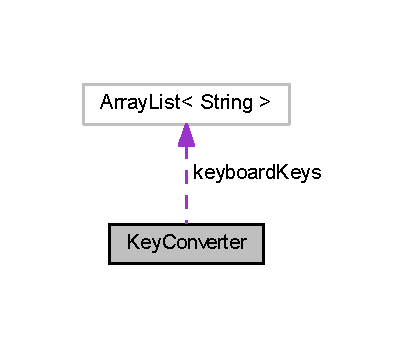
\includegraphics[width=196pt]{classcom_1_1lclion_1_1midiparser_1_1_key_converter__coll__graph}
\end{center}
\end{figure}
\subsection*{Public Member Functions}
\begin{DoxyCompactItemize}
\item 
\hyperlink{classcom_1_1lclion_1_1midiparser_1_1_key_converter_a9120cd6d8e70712293f11a7898c38f37}{Key\+Converter} ()
\item 
String \hyperlink{classcom_1_1lclion_1_1midiparser_1_1_key_converter_aa19949a61ff13647e0d76138ede95bf3}{convert\+Midi\+To\+Keyboard} (int midi\+Num)
\item 
int \hyperlink{classcom_1_1lclion_1_1midiparser_1_1_key_converter_a3d3303353cc49236c800b6ad8c6b7b1f}{convert\+Keyboard\+To\+Midi} (String keyboard\+Char)
\end{DoxyCompactItemize}
\subsection*{Private Member Functions}
\begin{DoxyCompactItemize}
\item 
void \hyperlink{classcom_1_1lclion_1_1midiparser_1_1_key_converter_a6d5d75a2ebe6d53c98735c6ce1f95241}{setup\+Default\+Keys} ()
\begin{DoxyCompactList}\small\item\em Setup default keys as question marks. \end{DoxyCompactList}\item 
void \hyperlink{classcom_1_1lclion_1_1midiparser_1_1_key_converter_a02fd73d861ef2e4aabb38c0c9ff82947}{init} ()
\end{DoxyCompactItemize}
\subsection*{Static Private Attributes}
\begin{DoxyCompactItemize}
\item 
static Array\+List$<$ String $>$ \hyperlink{classcom_1_1lclion_1_1midiparser_1_1_key_converter_af11968cbb98cd6af2f9346e917d7138d}{keyboard\+Keys} = new Array\+List$<$String$>$()
\end{DoxyCompactItemize}


\subsection{Detailed Description}
Convert M\+I\+D\+I Numbers to corresponding note key used in the Q\+W\+E\+R\+T\+Y keyboard. 

\begin{DoxyAuthor}{Author}
L\+C Lion 
\end{DoxyAuthor}


\subsection{Constructor \& Destructor Documentation}
\hypertarget{classcom_1_1lclion_1_1midiparser_1_1_key_converter_a9120cd6d8e70712293f11a7898c38f37}{\index{com\+::lclion\+::midiparser\+::\+Key\+Converter@{com\+::lclion\+::midiparser\+::\+Key\+Converter}!Key\+Converter@{Key\+Converter}}
\index{Key\+Converter@{Key\+Converter}!com\+::lclion\+::midiparser\+::\+Key\+Converter@{com\+::lclion\+::midiparser\+::\+Key\+Converter}}
\subsubsection[{Key\+Converter}]{\setlength{\rightskip}{0pt plus 5cm}{\bf Key\+Converter} (
\begin{DoxyParamCaption}
{}
\end{DoxyParamCaption}
)}}\label{classcom_1_1lclion_1_1midiparser_1_1_key_converter_a9120cd6d8e70712293f11a7898c38f37}


Here is the call graph for this function\+:\nopagebreak
\begin{figure}[H]
\begin{center}
\leavevmode
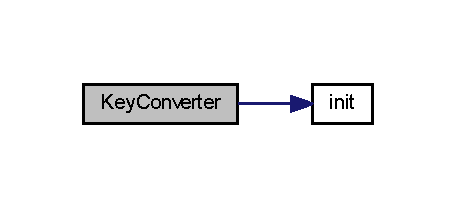
\includegraphics[width=219pt]{classcom_1_1lclion_1_1midiparser_1_1_key_converter_a9120cd6d8e70712293f11a7898c38f37_cgraph}
\end{center}
\end{figure}




\subsection{Member Function Documentation}
\hypertarget{classcom_1_1lclion_1_1midiparser_1_1_key_converter_a3d3303353cc49236c800b6ad8c6b7b1f}{\index{com\+::lclion\+::midiparser\+::\+Key\+Converter@{com\+::lclion\+::midiparser\+::\+Key\+Converter}!convert\+Keyboard\+To\+Midi@{convert\+Keyboard\+To\+Midi}}
\index{convert\+Keyboard\+To\+Midi@{convert\+Keyboard\+To\+Midi}!com\+::lclion\+::midiparser\+::\+Key\+Converter@{com\+::lclion\+::midiparser\+::\+Key\+Converter}}
\subsubsection[{convert\+Keyboard\+To\+Midi}]{\setlength{\rightskip}{0pt plus 5cm}int convert\+Keyboard\+To\+Midi (
\begin{DoxyParamCaption}
\item[{String}]{keyboard\+Char}
\end{DoxyParamCaption}
)}}\label{classcom_1_1lclion_1_1midiparser_1_1_key_converter_a3d3303353cc49236c800b6ad8c6b7b1f}
\hypertarget{classcom_1_1lclion_1_1midiparser_1_1_key_converter_aa19949a61ff13647e0d76138ede95bf3}{\index{com\+::lclion\+::midiparser\+::\+Key\+Converter@{com\+::lclion\+::midiparser\+::\+Key\+Converter}!convert\+Midi\+To\+Keyboard@{convert\+Midi\+To\+Keyboard}}
\index{convert\+Midi\+To\+Keyboard@{convert\+Midi\+To\+Keyboard}!com\+::lclion\+::midiparser\+::\+Key\+Converter@{com\+::lclion\+::midiparser\+::\+Key\+Converter}}
\subsubsection[{convert\+Midi\+To\+Keyboard}]{\setlength{\rightskip}{0pt plus 5cm}String convert\+Midi\+To\+Keyboard (
\begin{DoxyParamCaption}
\item[{int}]{midi\+Num}
\end{DoxyParamCaption}
)}}\label{classcom_1_1lclion_1_1midiparser_1_1_key_converter_aa19949a61ff13647e0d76138ede95bf3}
\hypertarget{classcom_1_1lclion_1_1midiparser_1_1_key_converter_a02fd73d861ef2e4aabb38c0c9ff82947}{\index{com\+::lclion\+::midiparser\+::\+Key\+Converter@{com\+::lclion\+::midiparser\+::\+Key\+Converter}!init@{init}}
\index{init@{init}!com\+::lclion\+::midiparser\+::\+Key\+Converter@{com\+::lclion\+::midiparser\+::\+Key\+Converter}}
\subsubsection[{init}]{\setlength{\rightskip}{0pt plus 5cm}void init (
\begin{DoxyParamCaption}
{}
\end{DoxyParamCaption}
)\hspace{0.3cm}{\ttfamily [private]}}}\label{classcom_1_1lclion_1_1midiparser_1_1_key_converter_a02fd73d861ef2e4aabb38c0c9ff82947}
\hypertarget{classcom_1_1lclion_1_1midiparser_1_1_key_converter_a6d5d75a2ebe6d53c98735c6ce1f95241}{\index{com\+::lclion\+::midiparser\+::\+Key\+Converter@{com\+::lclion\+::midiparser\+::\+Key\+Converter}!setup\+Default\+Keys@{setup\+Default\+Keys}}
\index{setup\+Default\+Keys@{setup\+Default\+Keys}!com\+::lclion\+::midiparser\+::\+Key\+Converter@{com\+::lclion\+::midiparser\+::\+Key\+Converter}}
\subsubsection[{setup\+Default\+Keys}]{\setlength{\rightskip}{0pt plus 5cm}void setup\+Default\+Keys (
\begin{DoxyParamCaption}
{}
\end{DoxyParamCaption}
)\hspace{0.3cm}{\ttfamily [private]}}}\label{classcom_1_1lclion_1_1midiparser_1_1_key_converter_a6d5d75a2ebe6d53c98735c6ce1f95241}


Setup default keys as question marks. 

If the requested keys are out of range, display a default question mark, indicating it is out of range. 

\subsection{Member Data Documentation}
\hypertarget{classcom_1_1lclion_1_1midiparser_1_1_key_converter_af11968cbb98cd6af2f9346e917d7138d}{\index{com\+::lclion\+::midiparser\+::\+Key\+Converter@{com\+::lclion\+::midiparser\+::\+Key\+Converter}!keyboard\+Keys@{keyboard\+Keys}}
\index{keyboard\+Keys@{keyboard\+Keys}!com\+::lclion\+::midiparser\+::\+Key\+Converter@{com\+::lclion\+::midiparser\+::\+Key\+Converter}}
\subsubsection[{keyboard\+Keys}]{\setlength{\rightskip}{0pt plus 5cm}Array\+List$<$String$>$ keyboard\+Keys = new Array\+List$<$String$>$()\hspace{0.3cm}{\ttfamily [static]}, {\ttfamily [private]}}}\label{classcom_1_1lclion_1_1midiparser_1_1_key_converter_af11968cbb98cd6af2f9346e917d7138d}


The documentation for this class was generated from the following file\+:\begin{DoxyCompactItemize}
\item 
src/com/lclion/midiparser/\hyperlink{_key_converter_8java}{Key\+Converter.\+java}\end{DoxyCompactItemize}

\hypertarget{classcom_1_1lclion_1_1midiparser_1_1_m_i_d_i_parser}{\section{M\+I\+D\+I\+Parser Class Reference}
\label{classcom_1_1lclion_1_1midiparser_1_1_m_i_d_i_parser}\index{M\+I\+D\+I\+Parser@{M\+I\+D\+I\+Parser}}
}


The main parser that parses M\+I\+D\+I file into readable notes.  




Collaboration diagram for M\+I\+D\+I\+Parser\+:\nopagebreak
\begin{figure}[H]
\begin{center}
\leavevmode
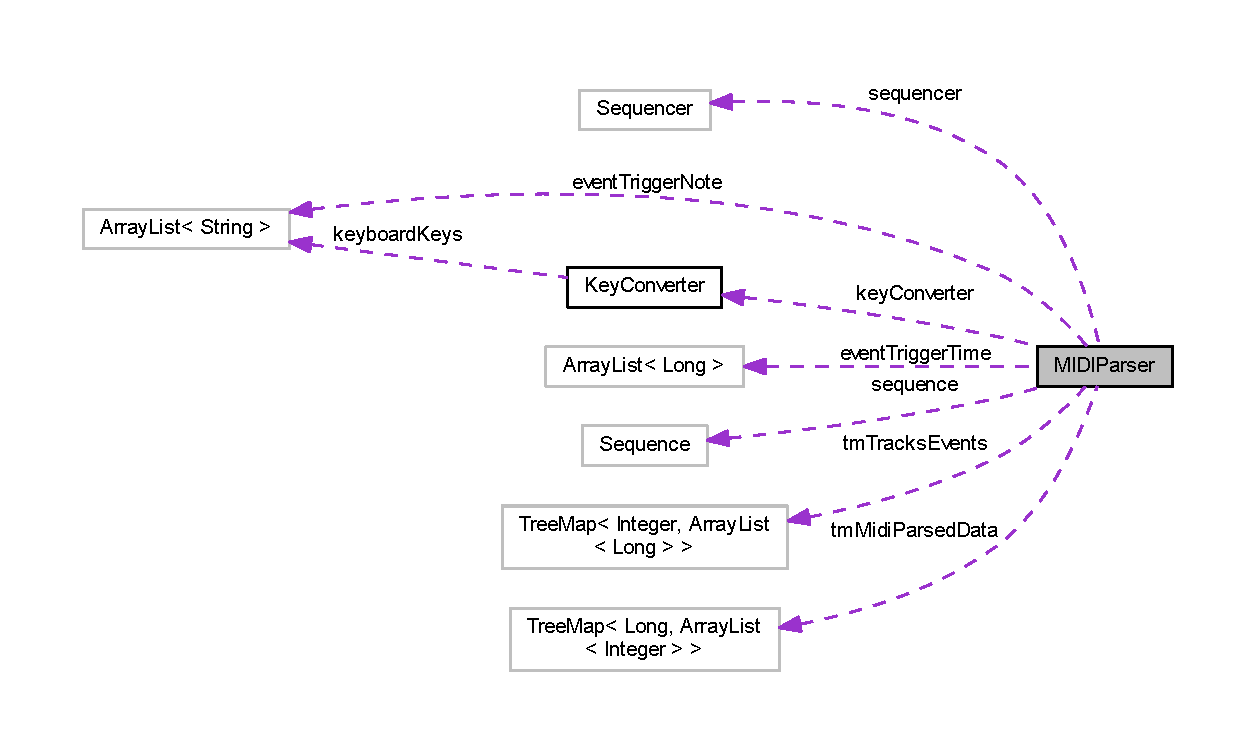
\includegraphics[width=350pt]{classcom_1_1lclion_1_1midiparser_1_1_m_i_d_i_parser__coll__graph}
\end{center}
\end{figure}
\subsection*{Public Member Functions}
\begin{DoxyCompactItemize}
\item 
\hyperlink{classcom_1_1lclion_1_1midiparser_1_1_m_i_d_i_parser_a42fc840125b67cc2511f12c7f6d1a362}{M\+I\+D\+I\+Parser} (File file)
\item 
String \hyperlink{classcom_1_1lclion_1_1midiparser_1_1_m_i_d_i_parser_a79cff8d5b2c0721d1871f65536fca8aa}{parse\+M\+I\+D\+I} ()
\item 
void \hyperlink{classcom_1_1lclion_1_1midiparser_1_1_m_i_d_i_parser_a6356cc4e4568eaf610999c4b32431749}{retrieve\+Midi\+Data} (int\mbox{[}$\,$\mbox{]} selected\+Tracks)
\item 
Tree\+Map$<$ Long, Array\+List\\*
$<$ Integer $>$ $>$ \hyperlink{classcom_1_1lclion_1_1midiparser_1_1_m_i_d_i_parser_af1c1599b923aa52978623f10a08d4d97}{get\+Tm\+Midi\+Parsed\+Data} ()
\item 
void \hyperlink{classcom_1_1lclion_1_1midiparser_1_1_m_i_d_i_parser_a31bfbd201be76f49735d3df6c362980a}{save\+Midi\+C\+S\+V} ()
\item 
String \hyperlink{classcom_1_1lclion_1_1midiparser_1_1_m_i_d_i_parser_ab52f7b2d5fc11fad840da51a5b49ab0e}{get\+Parsed\+Data} ()
\item 
Array\+List$<$ Integer $>$ \hyperlink{classcom_1_1lclion_1_1midiparser_1_1_m_i_d_i_parser_a5344cfe20b2847e6b1126b799c03e54e}{get\+Total\+Track\+Events\+Number} ()
\item 
Tree\+Map$<$ Integer, Array\+List\\*
$<$ Long $>$ $>$ \hyperlink{classcom_1_1lclion_1_1midiparser_1_1_m_i_d_i_parser_a25947e3c729a3eb6a7701dae3634b9b6}{retrieve\+Tracks\+Events} ()
\item 
int \hyperlink{classcom_1_1lclion_1_1midiparser_1_1_m_i_d_i_parser_a9ea2bab3f45e0b74eba2c08c635d4866}{get\+Patch\+Number} (int track\+Num)
\item 
int \hyperlink{classcom_1_1lclion_1_1midiparser_1_1_m_i_d_i_parser_aecc53ce49126b72aa5a52b01389b6e94}{get\+Channel\+Number} (int track\+Num)
\item 
Array\+List$<$ Long $>$ \hyperlink{classcom_1_1lclion_1_1midiparser_1_1_m_i_d_i_parser_aaa7385baef162e66f5dd608c345dda8d}{get\+Event\+Trigger\+Time} ()
\item 
long \hyperlink{classcom_1_1lclion_1_1midiparser_1_1_m_i_d_i_parser_a36449f95958a9f33a6bf44945252e2d7}{get\+Next\+Trigger\+Time} (int element\+Value)
\item 
String \hyperlink{classcom_1_1lclion_1_1midiparser_1_1_m_i_d_i_parser_a4669a62a8b0a61ee7cb351639cd5d357}{get\+Next\+Trigger\+Note} (int element\+Value)
\item 
int \hyperlink{classcom_1_1lclion_1_1midiparser_1_1_m_i_d_i_parser_acc6c9009b8fed2060c1b03fa051086d9}{get\+Next\+Trigger\+Time\+Element} (long tick)
\item 
long \hyperlink{classcom_1_1lclion_1_1midiparser_1_1_m_i_d_i_parser_aa9a3932117bdd0743daac84c2ca8e19a}{get\+Trigger\+Time\+Size} ()
\item 
long \hyperlink{classcom_1_1lclion_1_1midiparser_1_1_m_i_d_i_parser_a318c504fc464b620e829b6ed354cc922}{get\+Tick\+Length} ()
\item 
void \hyperlink{classcom_1_1lclion_1_1midiparser_1_1_m_i_d_i_parser_a6974b380083ade3bb6ce3d20a8f7592a}{set\+Measure\+Per\+Line} (int \hyperlink{classcom_1_1lclion_1_1midiparser_1_1_m_i_d_i_parser_a9a55cb81b8582eb4cbbc0a0ef91db56e}{measure\+Multiplier})
\item 
int \hyperlink{classcom_1_1lclion_1_1midiparser_1_1_m_i_d_i_parser_a0914f098f4ac38ddac1f9b57203a9241}{get\+Tracks} ()
\item 
int \hyperlink{classcom_1_1lclion_1_1midiparser_1_1_m_i_d_i_parser_a58cfc312af72ba770bca4aecc7e6c505}{get\+Quarter\+Note} ()
\end{DoxyCompactItemize}
\subsection*{Static Public Attributes}
\begin{DoxyCompactItemize}
\item 
static final int \hyperlink{classcom_1_1lclion_1_1midiparser_1_1_m_i_d_i_parser_ac4000b072e7a320337cc23bfc22de62d}{T\+I\+M\+E\+\_\+\+S\+I\+G\+N\+A\+T\+U\+R\+E} = 0x58
\end{DoxyCompactItemize}
\subsection*{Private Member Functions}
\begin{DoxyCompactItemize}
\item 
void \hyperlink{classcom_1_1lclion_1_1midiparser_1_1_m_i_d_i_parser_a95dc4fc863a442e4d13db55a30021dbc}{add\+Key} (char key\+To\+Add)
\item 
String \hyperlink{classcom_1_1lclion_1_1midiparser_1_1_m_i_d_i_parser_a0d273c8df789364bd05888eec0d887a1}{convert\+Midi\+Num\+To\+Keys} (Array\+List$<$ Integer $>$ M\+I\+D\+I\+Numbers)
\item 
String \hyperlink{classcom_1_1lclion_1_1midiparser_1_1_m_i_d_i_parser_a01a62f079f758bfd080cafec626e0bba}{format\+Brackets} (String current\+Notes)
\item 
String \hyperlink{classcom_1_1lclion_1_1midiparser_1_1_m_i_d_i_parser_aa721dfe0d567bb74d7d8b108cbd17989}{format\+Time} (long time, String current\+Notes)
\item 
void \hyperlink{classcom_1_1lclion_1_1midiparser_1_1_m_i_d_i_parser_a1a6947c3e60f6f74022834f05b71d8b3}{parse\+Data} (Tree\+Map$<$ Long, Array\+List$<$ Integer $>$$>$ raw\+Data)
\item 
void \hyperlink{classcom_1_1lclion_1_1midiparser_1_1_m_i_d_i_parser_a32e1f8f0f14a58552e8972fc6e02da30}{set\+Time\+Signature} ()
\item 
void \hyperlink{classcom_1_1lclion_1_1midiparser_1_1_m_i_d_i_parser_a0a6214124c40fd0db497cbdd73cf3a32}{get\+Time\+Signature} ()
\end{DoxyCompactItemize}
\subsection*{Private Attributes}
\begin{DoxyCompactItemize}
\item 
Sequencer \hyperlink{classcom_1_1lclion_1_1midiparser_1_1_m_i_d_i_parser_a857733a65a16f85598c03acd97305607}{sequencer} = null
\item 
Sequence \hyperlink{classcom_1_1lclion_1_1midiparser_1_1_m_i_d_i_parser_aae9bd69432c806ce0c10016839a874a2}{sequence} = null
\item 
String \hyperlink{classcom_1_1lclion_1_1midiparser_1_1_m_i_d_i_parser_a3a5f56162810aa1e371620c4c18cc82a}{file\+Name} = null
\item 
String \hyperlink{classcom_1_1lclion_1_1midiparser_1_1_m_i_d_i_parser_a9ade7b0db4d14601924d1d67a9a98c96}{str\+Time\+Signature\+Info} = null
\item 
String \hyperlink{classcom_1_1lclion_1_1midiparser_1_1_m_i_d_i_parser_a3c9243db1d16921999625d8c92137085}{complete\+Notes} = \char`\"{}\char`\"{}
\item 
Array\+List$<$ Long $>$ \hyperlink{classcom_1_1lclion_1_1midiparser_1_1_m_i_d_i_parser_a74fa4197a892bf1767a6e5eb295e00ab}{event\+Trigger\+Time} = new Array\+List$<$Long$>$()
\item 
Array\+List$<$ String $>$ \hyperlink{classcom_1_1lclion_1_1midiparser_1_1_m_i_d_i_parser_a3a6a37f76d1411625bac106b93d1c1b7}{event\+Trigger\+Note} = new Array\+List$<$String$>$()
\item 
Tree\+Map$<$ Long, Array\+List\\*
$<$ Integer $>$ $>$ \hyperlink{classcom_1_1lclion_1_1midiparser_1_1_m_i_d_i_parser_aaa5da6a46779f30b5e491729559ab183}{tm\+Midi\+Parsed\+Data} = null
\item 
Tree\+Map$<$ Integer, Array\+List\\*
$<$ Long $>$ $>$ \hyperlink{classcom_1_1lclion_1_1midiparser_1_1_m_i_d_i_parser_ac3ef5d55fe6e4c55e06efa4d6a4f05b3}{tm\+Tracks\+Events} = null
\item 
long \hyperlink{classcom_1_1lclion_1_1midiparser_1_1_m_i_d_i_parser_afe73b681d8322ca28bb66fab4764b310}{check\+Tick} = 0
\item 
long \hyperlink{classcom_1_1lclion_1_1midiparser_1_1_m_i_d_i_parser_aec0bccc7b1362ff3393cf1f13f0f89b1}{midi\+Tick\+Length} = 0
\item 
int \hyperlink{classcom_1_1lclion_1_1midiparser_1_1_m_i_d_i_parser_aa3851167fb02270887162e55dfb5d370}{beats\+Per\+Measure} = 0
\item 
int \hyperlink{classcom_1_1lclion_1_1midiparser_1_1_m_i_d_i_parser_ad1e462120d3438537d08dec3970bc996}{note\+Value\+In\+Measure} = 0
\item 
float \hyperlink{classcom_1_1lclion_1_1midiparser_1_1_m_i_d_i_parser_a77523469bbc99d657ddb184aa2dcb4c7}{measure\+Length} = 0
\item 
int \hyperlink{classcom_1_1lclion_1_1midiparser_1_1_m_i_d_i_parser_a9a55cb81b8582eb4cbbc0a0ef91db56e}{measure\+Multiplier} = 1
\item 
float \hyperlink{classcom_1_1lclion_1_1midiparser_1_1_m_i_d_i_parser_abd6a816e8fe161e38844aeddac581af2}{current\+Measure} = 0
\item 
String \hyperlink{classcom_1_1lclion_1_1midiparser_1_1_m_i_d_i_parser_af186165a05dd64dd883a4697fd0b1d00}{upper\+Keys} = \char`\"{}\char`\"{}
\item 
String \hyperlink{classcom_1_1lclion_1_1midiparser_1_1_m_i_d_i_parser_af2ff13695bae1b9c991aeaa6a7ad3f3c}{lower\+Keys} = \char`\"{}\char`\"{}
\item 
String \hyperlink{classcom_1_1lclion_1_1midiparser_1_1_m_i_d_i_parser_ae95a908b6894c33a614224f731a53b2d}{numeric\+Keys} = \char`\"{}\char`\"{}
\item 
String \hyperlink{classcom_1_1lclion_1_1midiparser_1_1_m_i_d_i_parser_abb638d880a4d9f3c793d9dfae2bd5d65}{other\+Keys} = \char`\"{}\char`\"{}
\end{DoxyCompactItemize}
\subsection*{Static Private Attributes}
\begin{DoxyCompactItemize}
\item 
static final int \hyperlink{classcom_1_1lclion_1_1midiparser_1_1_m_i_d_i_parser_ac035f42f6f27179d122b97d54fd030e1}{N\+O\+T\+E\+\_\+\+O\+N} = 0x90
\item 
static final int \hyperlink{classcom_1_1lclion_1_1midiparser_1_1_m_i_d_i_parser_ac6d1248a531a8620967406d69edda242}{N\+O\+T\+E\+\_\+\+O\+F\+F} = 0x80
\item 
static \hyperlink{classcom_1_1lclion_1_1midiparser_1_1_key_converter}{Key\+Converter} \hyperlink{classcom_1_1lclion_1_1midiparser_1_1_m_i_d_i_parser_acc7c29517d4ac6fb6eb51b8d9b714728}{key\+Converter} = new \hyperlink{classcom_1_1lclion_1_1midiparser_1_1_key_converter}{Key\+Converter}()
\end{DoxyCompactItemize}


\subsection{Detailed Description}
The main parser that parses M\+I\+D\+I file into readable notes. 

A class that parses M\+I\+D\+I Files directly, and outputs to alpha numeric keys.

\begin{DoxyAuthor}{Author}
L\+C Lion 
\end{DoxyAuthor}


\subsection{Constructor \& Destructor Documentation}
\hypertarget{classcom_1_1lclion_1_1midiparser_1_1_m_i_d_i_parser_a42fc840125b67cc2511f12c7f6d1a362}{\index{com\+::lclion\+::midiparser\+::\+M\+I\+D\+I\+Parser@{com\+::lclion\+::midiparser\+::\+M\+I\+D\+I\+Parser}!M\+I\+D\+I\+Parser@{M\+I\+D\+I\+Parser}}
\index{M\+I\+D\+I\+Parser@{M\+I\+D\+I\+Parser}!com\+::lclion\+::midiparser\+::\+M\+I\+D\+I\+Parser@{com\+::lclion\+::midiparser\+::\+M\+I\+D\+I\+Parser}}
\subsubsection[{M\+I\+D\+I\+Parser}]{\setlength{\rightskip}{0pt plus 5cm}{\bf M\+I\+D\+I\+Parser} (
\begin{DoxyParamCaption}
\item[{File}]{file}
\end{DoxyParamCaption}
)}}\label{classcom_1_1lclion_1_1midiparser_1_1_m_i_d_i_parser_a42fc840125b67cc2511f12c7f6d1a362}


\subsection{Member Function Documentation}
\hypertarget{classcom_1_1lclion_1_1midiparser_1_1_m_i_d_i_parser_a95dc4fc863a442e4d13db55a30021dbc}{\index{com\+::lclion\+::midiparser\+::\+M\+I\+D\+I\+Parser@{com\+::lclion\+::midiparser\+::\+M\+I\+D\+I\+Parser}!add\+Key@{add\+Key}}
\index{add\+Key@{add\+Key}!com\+::lclion\+::midiparser\+::\+M\+I\+D\+I\+Parser@{com\+::lclion\+::midiparser\+::\+M\+I\+D\+I\+Parser}}
\subsubsection[{add\+Key}]{\setlength{\rightskip}{0pt plus 5cm}void add\+Key (
\begin{DoxyParamCaption}
\item[{char}]{key\+To\+Add}
\end{DoxyParamCaption}
)\hspace{0.3cm}{\ttfamily [private]}}}\label{classcom_1_1lclion_1_1midiparser_1_1_m_i_d_i_parser_a95dc4fc863a442e4d13db55a30021dbc}
\hypertarget{classcom_1_1lclion_1_1midiparser_1_1_m_i_d_i_parser_a0d273c8df789364bd05888eec0d887a1}{\index{com\+::lclion\+::midiparser\+::\+M\+I\+D\+I\+Parser@{com\+::lclion\+::midiparser\+::\+M\+I\+D\+I\+Parser}!convert\+Midi\+Num\+To\+Keys@{convert\+Midi\+Num\+To\+Keys}}
\index{convert\+Midi\+Num\+To\+Keys@{convert\+Midi\+Num\+To\+Keys}!com\+::lclion\+::midiparser\+::\+M\+I\+D\+I\+Parser@{com\+::lclion\+::midiparser\+::\+M\+I\+D\+I\+Parser}}
\subsubsection[{convert\+Midi\+Num\+To\+Keys}]{\setlength{\rightskip}{0pt plus 5cm}String convert\+Midi\+Num\+To\+Keys (
\begin{DoxyParamCaption}
\item[{Array\+List$<$ Integer $>$}]{M\+I\+D\+I\+Numbers}
\end{DoxyParamCaption}
)\hspace{0.3cm}{\ttfamily [private]}}}\label{classcom_1_1lclion_1_1midiparser_1_1_m_i_d_i_parser_a0d273c8df789364bd05888eec0d887a1}


Here is the call graph for this function\+:\nopagebreak
\begin{figure}[H]
\begin{center}
\leavevmode
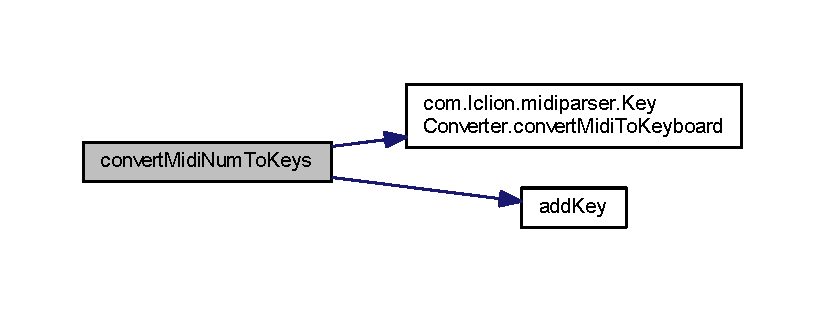
\includegraphics[width=350pt]{classcom_1_1lclion_1_1midiparser_1_1_m_i_d_i_parser_a0d273c8df789364bd05888eec0d887a1_cgraph}
\end{center}
\end{figure}


\hypertarget{classcom_1_1lclion_1_1midiparser_1_1_m_i_d_i_parser_a01a62f079f758bfd080cafec626e0bba}{\index{com\+::lclion\+::midiparser\+::\+M\+I\+D\+I\+Parser@{com\+::lclion\+::midiparser\+::\+M\+I\+D\+I\+Parser}!format\+Brackets@{format\+Brackets}}
\index{format\+Brackets@{format\+Brackets}!com\+::lclion\+::midiparser\+::\+M\+I\+D\+I\+Parser@{com\+::lclion\+::midiparser\+::\+M\+I\+D\+I\+Parser}}
\subsubsection[{format\+Brackets}]{\setlength{\rightskip}{0pt plus 5cm}String format\+Brackets (
\begin{DoxyParamCaption}
\item[{String}]{current\+Notes}
\end{DoxyParamCaption}
)\hspace{0.3cm}{\ttfamily [private]}}}\label{classcom_1_1lclion_1_1midiparser_1_1_m_i_d_i_parser_a01a62f079f758bfd080cafec626e0bba}
\hypertarget{classcom_1_1lclion_1_1midiparser_1_1_m_i_d_i_parser_aa721dfe0d567bb74d7d8b108cbd17989}{\index{com\+::lclion\+::midiparser\+::\+M\+I\+D\+I\+Parser@{com\+::lclion\+::midiparser\+::\+M\+I\+D\+I\+Parser}!format\+Time@{format\+Time}}
\index{format\+Time@{format\+Time}!com\+::lclion\+::midiparser\+::\+M\+I\+D\+I\+Parser@{com\+::lclion\+::midiparser\+::\+M\+I\+D\+I\+Parser}}
\subsubsection[{format\+Time}]{\setlength{\rightskip}{0pt plus 5cm}String format\+Time (
\begin{DoxyParamCaption}
\item[{long}]{time, }
\item[{String}]{current\+Notes}
\end{DoxyParamCaption}
)\hspace{0.3cm}{\ttfamily [private]}}}\label{classcom_1_1lclion_1_1midiparser_1_1_m_i_d_i_parser_aa721dfe0d567bb74d7d8b108cbd17989}
\hypertarget{classcom_1_1lclion_1_1midiparser_1_1_m_i_d_i_parser_aecc53ce49126b72aa5a52b01389b6e94}{\index{com\+::lclion\+::midiparser\+::\+M\+I\+D\+I\+Parser@{com\+::lclion\+::midiparser\+::\+M\+I\+D\+I\+Parser}!get\+Channel\+Number@{get\+Channel\+Number}}
\index{get\+Channel\+Number@{get\+Channel\+Number}!com\+::lclion\+::midiparser\+::\+M\+I\+D\+I\+Parser@{com\+::lclion\+::midiparser\+::\+M\+I\+D\+I\+Parser}}
\subsubsection[{get\+Channel\+Number}]{\setlength{\rightskip}{0pt plus 5cm}int get\+Channel\+Number (
\begin{DoxyParamCaption}
\item[{int}]{track\+Num}
\end{DoxyParamCaption}
)}}\label{classcom_1_1lclion_1_1midiparser_1_1_m_i_d_i_parser_aecc53ce49126b72aa5a52b01389b6e94}
\hypertarget{classcom_1_1lclion_1_1midiparser_1_1_m_i_d_i_parser_aaa7385baef162e66f5dd608c345dda8d}{\index{com\+::lclion\+::midiparser\+::\+M\+I\+D\+I\+Parser@{com\+::lclion\+::midiparser\+::\+M\+I\+D\+I\+Parser}!get\+Event\+Trigger\+Time@{get\+Event\+Trigger\+Time}}
\index{get\+Event\+Trigger\+Time@{get\+Event\+Trigger\+Time}!com\+::lclion\+::midiparser\+::\+M\+I\+D\+I\+Parser@{com\+::lclion\+::midiparser\+::\+M\+I\+D\+I\+Parser}}
\subsubsection[{get\+Event\+Trigger\+Time}]{\setlength{\rightskip}{0pt plus 5cm}Array\+List$<$Long$>$ get\+Event\+Trigger\+Time (
\begin{DoxyParamCaption}
{}
\end{DoxyParamCaption}
)}}\label{classcom_1_1lclion_1_1midiparser_1_1_m_i_d_i_parser_aaa7385baef162e66f5dd608c345dda8d}
\hypertarget{classcom_1_1lclion_1_1midiparser_1_1_m_i_d_i_parser_a4669a62a8b0a61ee7cb351639cd5d357}{\index{com\+::lclion\+::midiparser\+::\+M\+I\+D\+I\+Parser@{com\+::lclion\+::midiparser\+::\+M\+I\+D\+I\+Parser}!get\+Next\+Trigger\+Note@{get\+Next\+Trigger\+Note}}
\index{get\+Next\+Trigger\+Note@{get\+Next\+Trigger\+Note}!com\+::lclion\+::midiparser\+::\+M\+I\+D\+I\+Parser@{com\+::lclion\+::midiparser\+::\+M\+I\+D\+I\+Parser}}
\subsubsection[{get\+Next\+Trigger\+Note}]{\setlength{\rightskip}{0pt plus 5cm}String get\+Next\+Trigger\+Note (
\begin{DoxyParamCaption}
\item[{int}]{element\+Value}
\end{DoxyParamCaption}
)}}\label{classcom_1_1lclion_1_1midiparser_1_1_m_i_d_i_parser_a4669a62a8b0a61ee7cb351639cd5d357}
\hypertarget{classcom_1_1lclion_1_1midiparser_1_1_m_i_d_i_parser_a36449f95958a9f33a6bf44945252e2d7}{\index{com\+::lclion\+::midiparser\+::\+M\+I\+D\+I\+Parser@{com\+::lclion\+::midiparser\+::\+M\+I\+D\+I\+Parser}!get\+Next\+Trigger\+Time@{get\+Next\+Trigger\+Time}}
\index{get\+Next\+Trigger\+Time@{get\+Next\+Trigger\+Time}!com\+::lclion\+::midiparser\+::\+M\+I\+D\+I\+Parser@{com\+::lclion\+::midiparser\+::\+M\+I\+D\+I\+Parser}}
\subsubsection[{get\+Next\+Trigger\+Time}]{\setlength{\rightskip}{0pt plus 5cm}long get\+Next\+Trigger\+Time (
\begin{DoxyParamCaption}
\item[{int}]{element\+Value}
\end{DoxyParamCaption}
)}}\label{classcom_1_1lclion_1_1midiparser_1_1_m_i_d_i_parser_a36449f95958a9f33a6bf44945252e2d7}
\hypertarget{classcom_1_1lclion_1_1midiparser_1_1_m_i_d_i_parser_acc6c9009b8fed2060c1b03fa051086d9}{\index{com\+::lclion\+::midiparser\+::\+M\+I\+D\+I\+Parser@{com\+::lclion\+::midiparser\+::\+M\+I\+D\+I\+Parser}!get\+Next\+Trigger\+Time\+Element@{get\+Next\+Trigger\+Time\+Element}}
\index{get\+Next\+Trigger\+Time\+Element@{get\+Next\+Trigger\+Time\+Element}!com\+::lclion\+::midiparser\+::\+M\+I\+D\+I\+Parser@{com\+::lclion\+::midiparser\+::\+M\+I\+D\+I\+Parser}}
\subsubsection[{get\+Next\+Trigger\+Time\+Element}]{\setlength{\rightskip}{0pt plus 5cm}int get\+Next\+Trigger\+Time\+Element (
\begin{DoxyParamCaption}
\item[{long}]{tick}
\end{DoxyParamCaption}
)}}\label{classcom_1_1lclion_1_1midiparser_1_1_m_i_d_i_parser_acc6c9009b8fed2060c1b03fa051086d9}
\hypertarget{classcom_1_1lclion_1_1midiparser_1_1_m_i_d_i_parser_ab52f7b2d5fc11fad840da51a5b49ab0e}{\index{com\+::lclion\+::midiparser\+::\+M\+I\+D\+I\+Parser@{com\+::lclion\+::midiparser\+::\+M\+I\+D\+I\+Parser}!get\+Parsed\+Data@{get\+Parsed\+Data}}
\index{get\+Parsed\+Data@{get\+Parsed\+Data}!com\+::lclion\+::midiparser\+::\+M\+I\+D\+I\+Parser@{com\+::lclion\+::midiparser\+::\+M\+I\+D\+I\+Parser}}
\subsubsection[{get\+Parsed\+Data}]{\setlength{\rightskip}{0pt plus 5cm}String get\+Parsed\+Data (
\begin{DoxyParamCaption}
{}
\end{DoxyParamCaption}
)}}\label{classcom_1_1lclion_1_1midiparser_1_1_m_i_d_i_parser_ab52f7b2d5fc11fad840da51a5b49ab0e}
\hypertarget{classcom_1_1lclion_1_1midiparser_1_1_m_i_d_i_parser_a9ea2bab3f45e0b74eba2c08c635d4866}{\index{com\+::lclion\+::midiparser\+::\+M\+I\+D\+I\+Parser@{com\+::lclion\+::midiparser\+::\+M\+I\+D\+I\+Parser}!get\+Patch\+Number@{get\+Patch\+Number}}
\index{get\+Patch\+Number@{get\+Patch\+Number}!com\+::lclion\+::midiparser\+::\+M\+I\+D\+I\+Parser@{com\+::lclion\+::midiparser\+::\+M\+I\+D\+I\+Parser}}
\subsubsection[{get\+Patch\+Number}]{\setlength{\rightskip}{0pt plus 5cm}int get\+Patch\+Number (
\begin{DoxyParamCaption}
\item[{int}]{track\+Num}
\end{DoxyParamCaption}
)}}\label{classcom_1_1lclion_1_1midiparser_1_1_m_i_d_i_parser_a9ea2bab3f45e0b74eba2c08c635d4866}
\hypertarget{classcom_1_1lclion_1_1midiparser_1_1_m_i_d_i_parser_a58cfc312af72ba770bca4aecc7e6c505}{\index{com\+::lclion\+::midiparser\+::\+M\+I\+D\+I\+Parser@{com\+::lclion\+::midiparser\+::\+M\+I\+D\+I\+Parser}!get\+Quarter\+Note@{get\+Quarter\+Note}}
\index{get\+Quarter\+Note@{get\+Quarter\+Note}!com\+::lclion\+::midiparser\+::\+M\+I\+D\+I\+Parser@{com\+::lclion\+::midiparser\+::\+M\+I\+D\+I\+Parser}}
\subsubsection[{get\+Quarter\+Note}]{\setlength{\rightskip}{0pt plus 5cm}int get\+Quarter\+Note (
\begin{DoxyParamCaption}
{}
\end{DoxyParamCaption}
)}}\label{classcom_1_1lclion_1_1midiparser_1_1_m_i_d_i_parser_a58cfc312af72ba770bca4aecc7e6c505}
\hypertarget{classcom_1_1lclion_1_1midiparser_1_1_m_i_d_i_parser_a318c504fc464b620e829b6ed354cc922}{\index{com\+::lclion\+::midiparser\+::\+M\+I\+D\+I\+Parser@{com\+::lclion\+::midiparser\+::\+M\+I\+D\+I\+Parser}!get\+Tick\+Length@{get\+Tick\+Length}}
\index{get\+Tick\+Length@{get\+Tick\+Length}!com\+::lclion\+::midiparser\+::\+M\+I\+D\+I\+Parser@{com\+::lclion\+::midiparser\+::\+M\+I\+D\+I\+Parser}}
\subsubsection[{get\+Tick\+Length}]{\setlength{\rightskip}{0pt plus 5cm}long get\+Tick\+Length (
\begin{DoxyParamCaption}
{}
\end{DoxyParamCaption}
)}}\label{classcom_1_1lclion_1_1midiparser_1_1_m_i_d_i_parser_a318c504fc464b620e829b6ed354cc922}
\hypertarget{classcom_1_1lclion_1_1midiparser_1_1_m_i_d_i_parser_a0a6214124c40fd0db497cbdd73cf3a32}{\index{com\+::lclion\+::midiparser\+::\+M\+I\+D\+I\+Parser@{com\+::lclion\+::midiparser\+::\+M\+I\+D\+I\+Parser}!get\+Time\+Signature@{get\+Time\+Signature}}
\index{get\+Time\+Signature@{get\+Time\+Signature}!com\+::lclion\+::midiparser\+::\+M\+I\+D\+I\+Parser@{com\+::lclion\+::midiparser\+::\+M\+I\+D\+I\+Parser}}
\subsubsection[{get\+Time\+Signature}]{\setlength{\rightskip}{0pt plus 5cm}void get\+Time\+Signature (
\begin{DoxyParamCaption}
{}
\end{DoxyParamCaption}
)\hspace{0.3cm}{\ttfamily [private]}}}\label{classcom_1_1lclion_1_1midiparser_1_1_m_i_d_i_parser_a0a6214124c40fd0db497cbdd73cf3a32}
\hypertarget{classcom_1_1lclion_1_1midiparser_1_1_m_i_d_i_parser_af1c1599b923aa52978623f10a08d4d97}{\index{com\+::lclion\+::midiparser\+::\+M\+I\+D\+I\+Parser@{com\+::lclion\+::midiparser\+::\+M\+I\+D\+I\+Parser}!get\+Tm\+Midi\+Parsed\+Data@{get\+Tm\+Midi\+Parsed\+Data}}
\index{get\+Tm\+Midi\+Parsed\+Data@{get\+Tm\+Midi\+Parsed\+Data}!com\+::lclion\+::midiparser\+::\+M\+I\+D\+I\+Parser@{com\+::lclion\+::midiparser\+::\+M\+I\+D\+I\+Parser}}
\subsubsection[{get\+Tm\+Midi\+Parsed\+Data}]{\setlength{\rightskip}{0pt plus 5cm}Tree\+Map$<$Long, Array\+List$<$Integer$>$ $>$ get\+Tm\+Midi\+Parsed\+Data (
\begin{DoxyParamCaption}
{}
\end{DoxyParamCaption}
)}}\label{classcom_1_1lclion_1_1midiparser_1_1_m_i_d_i_parser_af1c1599b923aa52978623f10a08d4d97}
\hypertarget{classcom_1_1lclion_1_1midiparser_1_1_m_i_d_i_parser_a5344cfe20b2847e6b1126b799c03e54e}{\index{com\+::lclion\+::midiparser\+::\+M\+I\+D\+I\+Parser@{com\+::lclion\+::midiparser\+::\+M\+I\+D\+I\+Parser}!get\+Total\+Track\+Events\+Number@{get\+Total\+Track\+Events\+Number}}
\index{get\+Total\+Track\+Events\+Number@{get\+Total\+Track\+Events\+Number}!com\+::lclion\+::midiparser\+::\+M\+I\+D\+I\+Parser@{com\+::lclion\+::midiparser\+::\+M\+I\+D\+I\+Parser}}
\subsubsection[{get\+Total\+Track\+Events\+Number}]{\setlength{\rightskip}{0pt plus 5cm}Array\+List$<$Integer$>$ get\+Total\+Track\+Events\+Number (
\begin{DoxyParamCaption}
{}
\end{DoxyParamCaption}
)}}\label{classcom_1_1lclion_1_1midiparser_1_1_m_i_d_i_parser_a5344cfe20b2847e6b1126b799c03e54e}
Gets the total number of events in all tracks, through an arraylist \hypertarget{classcom_1_1lclion_1_1midiparser_1_1_m_i_d_i_parser_a0914f098f4ac38ddac1f9b57203a9241}{\index{com\+::lclion\+::midiparser\+::\+M\+I\+D\+I\+Parser@{com\+::lclion\+::midiparser\+::\+M\+I\+D\+I\+Parser}!get\+Tracks@{get\+Tracks}}
\index{get\+Tracks@{get\+Tracks}!com\+::lclion\+::midiparser\+::\+M\+I\+D\+I\+Parser@{com\+::lclion\+::midiparser\+::\+M\+I\+D\+I\+Parser}}
\subsubsection[{get\+Tracks}]{\setlength{\rightskip}{0pt plus 5cm}int get\+Tracks (
\begin{DoxyParamCaption}
{}
\end{DoxyParamCaption}
)}}\label{classcom_1_1lclion_1_1midiparser_1_1_m_i_d_i_parser_a0914f098f4ac38ddac1f9b57203a9241}
\hypertarget{classcom_1_1lclion_1_1midiparser_1_1_m_i_d_i_parser_aa9a3932117bdd0743daac84c2ca8e19a}{\index{com\+::lclion\+::midiparser\+::\+M\+I\+D\+I\+Parser@{com\+::lclion\+::midiparser\+::\+M\+I\+D\+I\+Parser}!get\+Trigger\+Time\+Size@{get\+Trigger\+Time\+Size}}
\index{get\+Trigger\+Time\+Size@{get\+Trigger\+Time\+Size}!com\+::lclion\+::midiparser\+::\+M\+I\+D\+I\+Parser@{com\+::lclion\+::midiparser\+::\+M\+I\+D\+I\+Parser}}
\subsubsection[{get\+Trigger\+Time\+Size}]{\setlength{\rightskip}{0pt plus 5cm}long get\+Trigger\+Time\+Size (
\begin{DoxyParamCaption}
{}
\end{DoxyParamCaption}
)}}\label{classcom_1_1lclion_1_1midiparser_1_1_m_i_d_i_parser_aa9a3932117bdd0743daac84c2ca8e19a}
\hypertarget{classcom_1_1lclion_1_1midiparser_1_1_m_i_d_i_parser_a1a6947c3e60f6f74022834f05b71d8b3}{\index{com\+::lclion\+::midiparser\+::\+M\+I\+D\+I\+Parser@{com\+::lclion\+::midiparser\+::\+M\+I\+D\+I\+Parser}!parse\+Data@{parse\+Data}}
\index{parse\+Data@{parse\+Data}!com\+::lclion\+::midiparser\+::\+M\+I\+D\+I\+Parser@{com\+::lclion\+::midiparser\+::\+M\+I\+D\+I\+Parser}}
\subsubsection[{parse\+Data}]{\setlength{\rightskip}{0pt plus 5cm}void parse\+Data (
\begin{DoxyParamCaption}
\item[{Tree\+Map$<$ Long, Array\+List$<$ Integer $>$$>$}]{raw\+Data}
\end{DoxyParamCaption}
)\hspace{0.3cm}{\ttfamily [private]}}}\label{classcom_1_1lclion_1_1midiparser_1_1_m_i_d_i_parser_a1a6947c3e60f6f74022834f05b71d8b3}


Here is the call graph for this function\+:\nopagebreak
\begin{figure}[H]
\begin{center}
\leavevmode
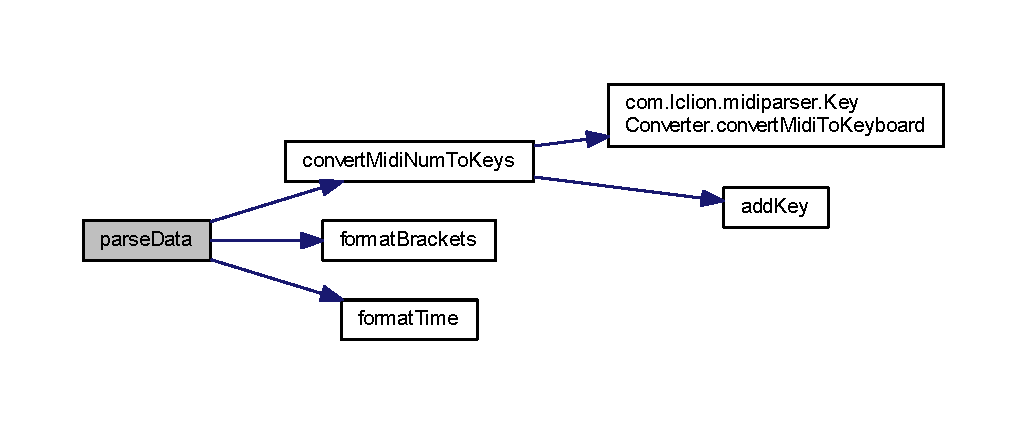
\includegraphics[width=350pt]{classcom_1_1lclion_1_1midiparser_1_1_m_i_d_i_parser_a1a6947c3e60f6f74022834f05b71d8b3_cgraph}
\end{center}
\end{figure}


\hypertarget{classcom_1_1lclion_1_1midiparser_1_1_m_i_d_i_parser_a79cff8d5b2c0721d1871f65536fca8aa}{\index{com\+::lclion\+::midiparser\+::\+M\+I\+D\+I\+Parser@{com\+::lclion\+::midiparser\+::\+M\+I\+D\+I\+Parser}!parse\+M\+I\+D\+I@{parse\+M\+I\+D\+I}}
\index{parse\+M\+I\+D\+I@{parse\+M\+I\+D\+I}!com\+::lclion\+::midiparser\+::\+M\+I\+D\+I\+Parser@{com\+::lclion\+::midiparser\+::\+M\+I\+D\+I\+Parser}}
\subsubsection[{parse\+M\+I\+D\+I}]{\setlength{\rightskip}{0pt plus 5cm}String parse\+M\+I\+D\+I (
\begin{DoxyParamCaption}
{}
\end{DoxyParamCaption}
)}}\label{classcom_1_1lclion_1_1midiparser_1_1_m_i_d_i_parser_a79cff8d5b2c0721d1871f65536fca8aa}
The main M\+I\+D\+I parse loop logic Extracts necessary data from the M\+I\+D\+I, and converts them to Computer Keyboard Keys. It also saves the parsed midi data to a .csv file for my autoplay script. Complies with Midi\+C\+S\+V-\/1.\+1 output format for more information about the formatting of passed M\+I\+D\+I data, visit \href{http://www.fourmilab.ch/webtools/midicsv/}{\tt http\+://www.\+fourmilab.\+ch/webtools/midicsv/} This class is in the process of deprecation, following D\+R\+Y principles (Takes too long to parse)

\begin{DoxyReturn}{Returns}
the parsed notes in String 
\end{DoxyReturn}


Here is the call graph for this function\+:\nopagebreak
\begin{figure}[H]
\begin{center}
\leavevmode
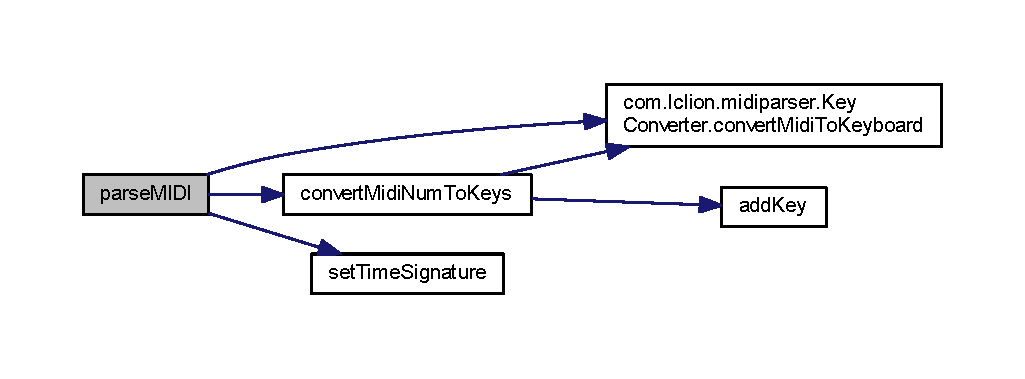
\includegraphics[width=350pt]{classcom_1_1lclion_1_1midiparser_1_1_m_i_d_i_parser_a79cff8d5b2c0721d1871f65536fca8aa_cgraph}
\end{center}
\end{figure}


\hypertarget{classcom_1_1lclion_1_1midiparser_1_1_m_i_d_i_parser_a6356cc4e4568eaf610999c4b32431749}{\index{com\+::lclion\+::midiparser\+::\+M\+I\+D\+I\+Parser@{com\+::lclion\+::midiparser\+::\+M\+I\+D\+I\+Parser}!retrieve\+Midi\+Data@{retrieve\+Midi\+Data}}
\index{retrieve\+Midi\+Data@{retrieve\+Midi\+Data}!com\+::lclion\+::midiparser\+::\+M\+I\+D\+I\+Parser@{com\+::lclion\+::midiparser\+::\+M\+I\+D\+I\+Parser}}
\subsubsection[{retrieve\+Midi\+Data}]{\setlength{\rightskip}{0pt plus 5cm}void retrieve\+Midi\+Data (
\begin{DoxyParamCaption}
\item[{int\mbox{[}$\,$\mbox{]}}]{selected\+Tracks}
\end{DoxyParamCaption}
)}}\label{classcom_1_1lclion_1_1midiparser_1_1_m_i_d_i_parser_a6356cc4e4568eaf610999c4b32431749}
Retrieve the timing information of M\+I\+D\+I Events that has Note On, and all subsequential notes that are played on that time. The data is stored in a Tree\+Map


\begin{DoxyParams}{Parameters}
{\em selected\+Tracks} & The selected tracks from the midi. If an empty array is passed (as null), it will parse all tracks \\
\hline
\end{DoxyParams}


Here is the call graph for this function\+:\nopagebreak
\begin{figure}[H]
\begin{center}
\leavevmode
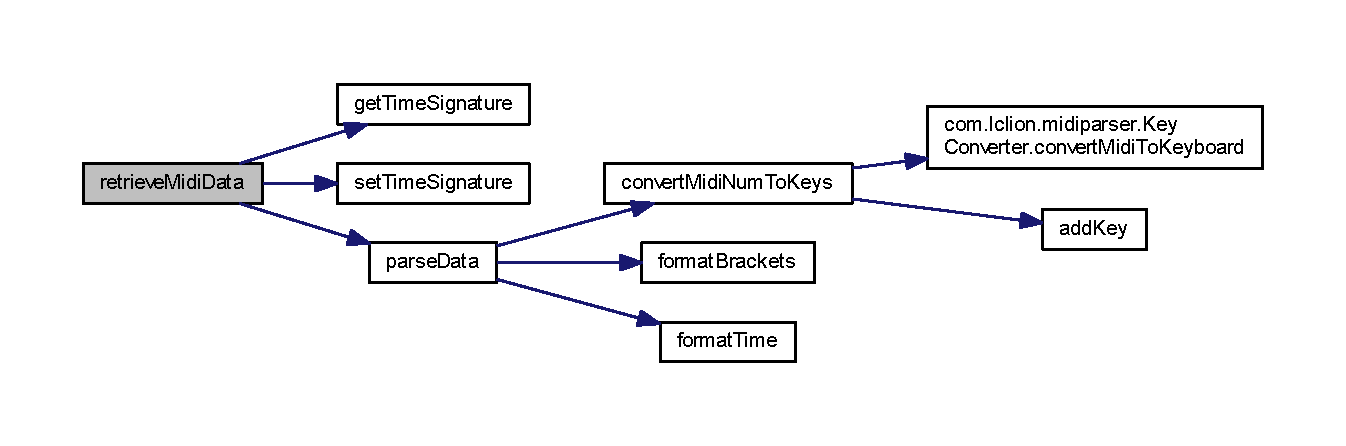
\includegraphics[width=350pt]{classcom_1_1lclion_1_1midiparser_1_1_m_i_d_i_parser_a6356cc4e4568eaf610999c4b32431749_cgraph}
\end{center}
\end{figure}


\hypertarget{classcom_1_1lclion_1_1midiparser_1_1_m_i_d_i_parser_a25947e3c729a3eb6a7701dae3634b9b6}{\index{com\+::lclion\+::midiparser\+::\+M\+I\+D\+I\+Parser@{com\+::lclion\+::midiparser\+::\+M\+I\+D\+I\+Parser}!retrieve\+Tracks\+Events@{retrieve\+Tracks\+Events}}
\index{retrieve\+Tracks\+Events@{retrieve\+Tracks\+Events}!com\+::lclion\+::midiparser\+::\+M\+I\+D\+I\+Parser@{com\+::lclion\+::midiparser\+::\+M\+I\+D\+I\+Parser}}
\subsubsection[{retrieve\+Tracks\+Events}]{\setlength{\rightskip}{0pt plus 5cm}Tree\+Map$<$Integer, Array\+List$<$Long$>$ $>$ retrieve\+Tracks\+Events (
\begin{DoxyParamCaption}
{}
\end{DoxyParamCaption}
)}}\label{classcom_1_1lclion_1_1midiparser_1_1_m_i_d_i_parser_a25947e3c729a3eb6a7701dae3634b9b6}
Returns the total number of events in all tracks, through a Tree\+Map Tree\+Map\+: $<$\+Key$>$, 

Key\+: The track number in Integer. Track starts at 1, not zero. Value\+: An Array\+List of all events in that track. \hypertarget{classcom_1_1lclion_1_1midiparser_1_1_m_i_d_i_parser_a31bfbd201be76f49735d3df6c362980a}{\index{com\+::lclion\+::midiparser\+::\+M\+I\+D\+I\+Parser@{com\+::lclion\+::midiparser\+::\+M\+I\+D\+I\+Parser}!save\+Midi\+C\+S\+V@{save\+Midi\+C\+S\+V}}
\index{save\+Midi\+C\+S\+V@{save\+Midi\+C\+S\+V}!com\+::lclion\+::midiparser\+::\+M\+I\+D\+I\+Parser@{com\+::lclion\+::midiparser\+::\+M\+I\+D\+I\+Parser}}
\subsubsection[{save\+Midi\+C\+S\+V}]{\setlength{\rightskip}{0pt plus 5cm}void save\+Midi\+C\+S\+V (
\begin{DoxyParamCaption}
{}
\end{DoxyParamCaption}
)}}\label{classcom_1_1lclion_1_1midiparser_1_1_m_i_d_i_parser_a31bfbd201be76f49735d3df6c362980a}
For the selected midi, output a .csv file containing parsed midi data for Note\+\_\+on events only. the csv is used in scripts and is not used in this program It strictly follows the Midi\+C\+S\+V1-\/1 output conventions for more information regarding the convention format used, visit \href{http://www.fourmilab.ch/webtools/midicsv/}{\tt http\+://www.\+fourmilab.\+ch/webtools/midicsv/} \hypertarget{classcom_1_1lclion_1_1midiparser_1_1_m_i_d_i_parser_a6974b380083ade3bb6ce3d20a8f7592a}{\index{com\+::lclion\+::midiparser\+::\+M\+I\+D\+I\+Parser@{com\+::lclion\+::midiparser\+::\+M\+I\+D\+I\+Parser}!set\+Measure\+Per\+Line@{set\+Measure\+Per\+Line}}
\index{set\+Measure\+Per\+Line@{set\+Measure\+Per\+Line}!com\+::lclion\+::midiparser\+::\+M\+I\+D\+I\+Parser@{com\+::lclion\+::midiparser\+::\+M\+I\+D\+I\+Parser}}
\subsubsection[{set\+Measure\+Per\+Line}]{\setlength{\rightskip}{0pt plus 5cm}void set\+Measure\+Per\+Line (
\begin{DoxyParamCaption}
\item[{int}]{measure\+Multiplier}
\end{DoxyParamCaption}
)}}\label{classcom_1_1lclion_1_1midiparser_1_1_m_i_d_i_parser_a6974b380083ade3bb6ce3d20a8f7592a}


Here is the call graph for this function\+:\nopagebreak
\begin{figure}[H]
\begin{center}
\leavevmode
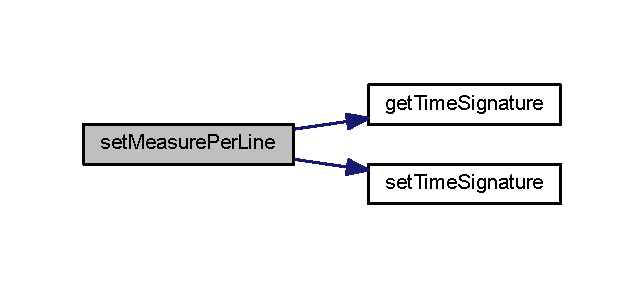
\includegraphics[width=309pt]{classcom_1_1lclion_1_1midiparser_1_1_m_i_d_i_parser_a6974b380083ade3bb6ce3d20a8f7592a_cgraph}
\end{center}
\end{figure}


\hypertarget{classcom_1_1lclion_1_1midiparser_1_1_m_i_d_i_parser_a32e1f8f0f14a58552e8972fc6e02da30}{\index{com\+::lclion\+::midiparser\+::\+M\+I\+D\+I\+Parser@{com\+::lclion\+::midiparser\+::\+M\+I\+D\+I\+Parser}!set\+Time\+Signature@{set\+Time\+Signature}}
\index{set\+Time\+Signature@{set\+Time\+Signature}!com\+::lclion\+::midiparser\+::\+M\+I\+D\+I\+Parser@{com\+::lclion\+::midiparser\+::\+M\+I\+D\+I\+Parser}}
\subsubsection[{set\+Time\+Signature}]{\setlength{\rightskip}{0pt plus 5cm}void set\+Time\+Signature (
\begin{DoxyParamCaption}
{}
\end{DoxyParamCaption}
)\hspace{0.3cm}{\ttfamily [private]}}}\label{classcom_1_1lclion_1_1midiparser_1_1_m_i_d_i_parser_a32e1f8f0f14a58552e8972fc6e02da30}


\subsection{Member Data Documentation}
\hypertarget{classcom_1_1lclion_1_1midiparser_1_1_m_i_d_i_parser_aa3851167fb02270887162e55dfb5d370}{\index{com\+::lclion\+::midiparser\+::\+M\+I\+D\+I\+Parser@{com\+::lclion\+::midiparser\+::\+M\+I\+D\+I\+Parser}!beats\+Per\+Measure@{beats\+Per\+Measure}}
\index{beats\+Per\+Measure@{beats\+Per\+Measure}!com\+::lclion\+::midiparser\+::\+M\+I\+D\+I\+Parser@{com\+::lclion\+::midiparser\+::\+M\+I\+D\+I\+Parser}}
\subsubsection[{beats\+Per\+Measure}]{\setlength{\rightskip}{0pt plus 5cm}int beats\+Per\+Measure = 0\hspace{0.3cm}{\ttfamily [private]}}}\label{classcom_1_1lclion_1_1midiparser_1_1_m_i_d_i_parser_aa3851167fb02270887162e55dfb5d370}
\hypertarget{classcom_1_1lclion_1_1midiparser_1_1_m_i_d_i_parser_afe73b681d8322ca28bb66fab4764b310}{\index{com\+::lclion\+::midiparser\+::\+M\+I\+D\+I\+Parser@{com\+::lclion\+::midiparser\+::\+M\+I\+D\+I\+Parser}!check\+Tick@{check\+Tick}}
\index{check\+Tick@{check\+Tick}!com\+::lclion\+::midiparser\+::\+M\+I\+D\+I\+Parser@{com\+::lclion\+::midiparser\+::\+M\+I\+D\+I\+Parser}}
\subsubsection[{check\+Tick}]{\setlength{\rightskip}{0pt plus 5cm}long check\+Tick = 0\hspace{0.3cm}{\ttfamily [private]}}}\label{classcom_1_1lclion_1_1midiparser_1_1_m_i_d_i_parser_afe73b681d8322ca28bb66fab4764b310}
\hypertarget{classcom_1_1lclion_1_1midiparser_1_1_m_i_d_i_parser_a3c9243db1d16921999625d8c92137085}{\index{com\+::lclion\+::midiparser\+::\+M\+I\+D\+I\+Parser@{com\+::lclion\+::midiparser\+::\+M\+I\+D\+I\+Parser}!complete\+Notes@{complete\+Notes}}
\index{complete\+Notes@{complete\+Notes}!com\+::lclion\+::midiparser\+::\+M\+I\+D\+I\+Parser@{com\+::lclion\+::midiparser\+::\+M\+I\+D\+I\+Parser}}
\subsubsection[{complete\+Notes}]{\setlength{\rightskip}{0pt plus 5cm}String complete\+Notes = \char`\"{}\char`\"{}\hspace{0.3cm}{\ttfamily [private]}}}\label{classcom_1_1lclion_1_1midiparser_1_1_m_i_d_i_parser_a3c9243db1d16921999625d8c92137085}
\hypertarget{classcom_1_1lclion_1_1midiparser_1_1_m_i_d_i_parser_abd6a816e8fe161e38844aeddac581af2}{\index{com\+::lclion\+::midiparser\+::\+M\+I\+D\+I\+Parser@{com\+::lclion\+::midiparser\+::\+M\+I\+D\+I\+Parser}!current\+Measure@{current\+Measure}}
\index{current\+Measure@{current\+Measure}!com\+::lclion\+::midiparser\+::\+M\+I\+D\+I\+Parser@{com\+::lclion\+::midiparser\+::\+M\+I\+D\+I\+Parser}}
\subsubsection[{current\+Measure}]{\setlength{\rightskip}{0pt plus 5cm}float current\+Measure = 0\hspace{0.3cm}{\ttfamily [private]}}}\label{classcom_1_1lclion_1_1midiparser_1_1_m_i_d_i_parser_abd6a816e8fe161e38844aeddac581af2}
\hypertarget{classcom_1_1lclion_1_1midiparser_1_1_m_i_d_i_parser_a3a6a37f76d1411625bac106b93d1c1b7}{\index{com\+::lclion\+::midiparser\+::\+M\+I\+D\+I\+Parser@{com\+::lclion\+::midiparser\+::\+M\+I\+D\+I\+Parser}!event\+Trigger\+Note@{event\+Trigger\+Note}}
\index{event\+Trigger\+Note@{event\+Trigger\+Note}!com\+::lclion\+::midiparser\+::\+M\+I\+D\+I\+Parser@{com\+::lclion\+::midiparser\+::\+M\+I\+D\+I\+Parser}}
\subsubsection[{event\+Trigger\+Note}]{\setlength{\rightskip}{0pt plus 5cm}Array\+List$<$String$>$ event\+Trigger\+Note = new Array\+List$<$String$>$()\hspace{0.3cm}{\ttfamily [private]}}}\label{classcom_1_1lclion_1_1midiparser_1_1_m_i_d_i_parser_a3a6a37f76d1411625bac106b93d1c1b7}
\hypertarget{classcom_1_1lclion_1_1midiparser_1_1_m_i_d_i_parser_a74fa4197a892bf1767a6e5eb295e00ab}{\index{com\+::lclion\+::midiparser\+::\+M\+I\+D\+I\+Parser@{com\+::lclion\+::midiparser\+::\+M\+I\+D\+I\+Parser}!event\+Trigger\+Time@{event\+Trigger\+Time}}
\index{event\+Trigger\+Time@{event\+Trigger\+Time}!com\+::lclion\+::midiparser\+::\+M\+I\+D\+I\+Parser@{com\+::lclion\+::midiparser\+::\+M\+I\+D\+I\+Parser}}
\subsubsection[{event\+Trigger\+Time}]{\setlength{\rightskip}{0pt plus 5cm}Array\+List$<$Long$>$ event\+Trigger\+Time = new Array\+List$<$Long$>$()\hspace{0.3cm}{\ttfamily [private]}}}\label{classcom_1_1lclion_1_1midiparser_1_1_m_i_d_i_parser_a74fa4197a892bf1767a6e5eb295e00ab}
\hypertarget{classcom_1_1lclion_1_1midiparser_1_1_m_i_d_i_parser_a3a5f56162810aa1e371620c4c18cc82a}{\index{com\+::lclion\+::midiparser\+::\+M\+I\+D\+I\+Parser@{com\+::lclion\+::midiparser\+::\+M\+I\+D\+I\+Parser}!file\+Name@{file\+Name}}
\index{file\+Name@{file\+Name}!com\+::lclion\+::midiparser\+::\+M\+I\+D\+I\+Parser@{com\+::lclion\+::midiparser\+::\+M\+I\+D\+I\+Parser}}
\subsubsection[{file\+Name}]{\setlength{\rightskip}{0pt plus 5cm}String file\+Name = null\hspace{0.3cm}{\ttfamily [private]}}}\label{classcom_1_1lclion_1_1midiparser_1_1_m_i_d_i_parser_a3a5f56162810aa1e371620c4c18cc82a}
\hypertarget{classcom_1_1lclion_1_1midiparser_1_1_m_i_d_i_parser_acc7c29517d4ac6fb6eb51b8d9b714728}{\index{com\+::lclion\+::midiparser\+::\+M\+I\+D\+I\+Parser@{com\+::lclion\+::midiparser\+::\+M\+I\+D\+I\+Parser}!key\+Converter@{key\+Converter}}
\index{key\+Converter@{key\+Converter}!com\+::lclion\+::midiparser\+::\+M\+I\+D\+I\+Parser@{com\+::lclion\+::midiparser\+::\+M\+I\+D\+I\+Parser}}
\subsubsection[{key\+Converter}]{\setlength{\rightskip}{0pt plus 5cm}{\bf Key\+Converter} key\+Converter = new {\bf Key\+Converter}()\hspace{0.3cm}{\ttfamily [static]}, {\ttfamily [private]}}}\label{classcom_1_1lclion_1_1midiparser_1_1_m_i_d_i_parser_acc7c29517d4ac6fb6eb51b8d9b714728}
\hypertarget{classcom_1_1lclion_1_1midiparser_1_1_m_i_d_i_parser_af2ff13695bae1b9c991aeaa6a7ad3f3c}{\index{com\+::lclion\+::midiparser\+::\+M\+I\+D\+I\+Parser@{com\+::lclion\+::midiparser\+::\+M\+I\+D\+I\+Parser}!lower\+Keys@{lower\+Keys}}
\index{lower\+Keys@{lower\+Keys}!com\+::lclion\+::midiparser\+::\+M\+I\+D\+I\+Parser@{com\+::lclion\+::midiparser\+::\+M\+I\+D\+I\+Parser}}
\subsubsection[{lower\+Keys}]{\setlength{\rightskip}{0pt plus 5cm}String lower\+Keys = \char`\"{}\char`\"{}\hspace{0.3cm}{\ttfamily [private]}}}\label{classcom_1_1lclion_1_1midiparser_1_1_m_i_d_i_parser_af2ff13695bae1b9c991aeaa6a7ad3f3c}
\hypertarget{classcom_1_1lclion_1_1midiparser_1_1_m_i_d_i_parser_a77523469bbc99d657ddb184aa2dcb4c7}{\index{com\+::lclion\+::midiparser\+::\+M\+I\+D\+I\+Parser@{com\+::lclion\+::midiparser\+::\+M\+I\+D\+I\+Parser}!measure\+Length@{measure\+Length}}
\index{measure\+Length@{measure\+Length}!com\+::lclion\+::midiparser\+::\+M\+I\+D\+I\+Parser@{com\+::lclion\+::midiparser\+::\+M\+I\+D\+I\+Parser}}
\subsubsection[{measure\+Length}]{\setlength{\rightskip}{0pt plus 5cm}float measure\+Length = 0\hspace{0.3cm}{\ttfamily [private]}}}\label{classcom_1_1lclion_1_1midiparser_1_1_m_i_d_i_parser_a77523469bbc99d657ddb184aa2dcb4c7}
\hypertarget{classcom_1_1lclion_1_1midiparser_1_1_m_i_d_i_parser_a9a55cb81b8582eb4cbbc0a0ef91db56e}{\index{com\+::lclion\+::midiparser\+::\+M\+I\+D\+I\+Parser@{com\+::lclion\+::midiparser\+::\+M\+I\+D\+I\+Parser}!measure\+Multiplier@{measure\+Multiplier}}
\index{measure\+Multiplier@{measure\+Multiplier}!com\+::lclion\+::midiparser\+::\+M\+I\+D\+I\+Parser@{com\+::lclion\+::midiparser\+::\+M\+I\+D\+I\+Parser}}
\subsubsection[{measure\+Multiplier}]{\setlength{\rightskip}{0pt plus 5cm}int measure\+Multiplier = 1\hspace{0.3cm}{\ttfamily [private]}}}\label{classcom_1_1lclion_1_1midiparser_1_1_m_i_d_i_parser_a9a55cb81b8582eb4cbbc0a0ef91db56e}
\hypertarget{classcom_1_1lclion_1_1midiparser_1_1_m_i_d_i_parser_aec0bccc7b1362ff3393cf1f13f0f89b1}{\index{com\+::lclion\+::midiparser\+::\+M\+I\+D\+I\+Parser@{com\+::lclion\+::midiparser\+::\+M\+I\+D\+I\+Parser}!midi\+Tick\+Length@{midi\+Tick\+Length}}
\index{midi\+Tick\+Length@{midi\+Tick\+Length}!com\+::lclion\+::midiparser\+::\+M\+I\+D\+I\+Parser@{com\+::lclion\+::midiparser\+::\+M\+I\+D\+I\+Parser}}
\subsubsection[{midi\+Tick\+Length}]{\setlength{\rightskip}{0pt plus 5cm}long midi\+Tick\+Length = 0\hspace{0.3cm}{\ttfamily [private]}}}\label{classcom_1_1lclion_1_1midiparser_1_1_m_i_d_i_parser_aec0bccc7b1362ff3393cf1f13f0f89b1}
\hypertarget{classcom_1_1lclion_1_1midiparser_1_1_m_i_d_i_parser_ac6d1248a531a8620967406d69edda242}{\index{com\+::lclion\+::midiparser\+::\+M\+I\+D\+I\+Parser@{com\+::lclion\+::midiparser\+::\+M\+I\+D\+I\+Parser}!N\+O\+T\+E\+\_\+\+O\+F\+F@{N\+O\+T\+E\+\_\+\+O\+F\+F}}
\index{N\+O\+T\+E\+\_\+\+O\+F\+F@{N\+O\+T\+E\+\_\+\+O\+F\+F}!com\+::lclion\+::midiparser\+::\+M\+I\+D\+I\+Parser@{com\+::lclion\+::midiparser\+::\+M\+I\+D\+I\+Parser}}
\subsubsection[{N\+O\+T\+E\+\_\+\+O\+F\+F}]{\setlength{\rightskip}{0pt plus 5cm}final int N\+O\+T\+E\+\_\+\+O\+F\+F = 0x80\hspace{0.3cm}{\ttfamily [static]}, {\ttfamily [private]}}}\label{classcom_1_1lclion_1_1midiparser_1_1_m_i_d_i_parser_ac6d1248a531a8620967406d69edda242}
\hypertarget{classcom_1_1lclion_1_1midiparser_1_1_m_i_d_i_parser_ac035f42f6f27179d122b97d54fd030e1}{\index{com\+::lclion\+::midiparser\+::\+M\+I\+D\+I\+Parser@{com\+::lclion\+::midiparser\+::\+M\+I\+D\+I\+Parser}!N\+O\+T\+E\+\_\+\+O\+N@{N\+O\+T\+E\+\_\+\+O\+N}}
\index{N\+O\+T\+E\+\_\+\+O\+N@{N\+O\+T\+E\+\_\+\+O\+N}!com\+::lclion\+::midiparser\+::\+M\+I\+D\+I\+Parser@{com\+::lclion\+::midiparser\+::\+M\+I\+D\+I\+Parser}}
\subsubsection[{N\+O\+T\+E\+\_\+\+O\+N}]{\setlength{\rightskip}{0pt plus 5cm}final int N\+O\+T\+E\+\_\+\+O\+N = 0x90\hspace{0.3cm}{\ttfamily [static]}, {\ttfamily [private]}}}\label{classcom_1_1lclion_1_1midiparser_1_1_m_i_d_i_parser_ac035f42f6f27179d122b97d54fd030e1}
\hypertarget{classcom_1_1lclion_1_1midiparser_1_1_m_i_d_i_parser_ad1e462120d3438537d08dec3970bc996}{\index{com\+::lclion\+::midiparser\+::\+M\+I\+D\+I\+Parser@{com\+::lclion\+::midiparser\+::\+M\+I\+D\+I\+Parser}!note\+Value\+In\+Measure@{note\+Value\+In\+Measure}}
\index{note\+Value\+In\+Measure@{note\+Value\+In\+Measure}!com\+::lclion\+::midiparser\+::\+M\+I\+D\+I\+Parser@{com\+::lclion\+::midiparser\+::\+M\+I\+D\+I\+Parser}}
\subsubsection[{note\+Value\+In\+Measure}]{\setlength{\rightskip}{0pt plus 5cm}int note\+Value\+In\+Measure = 0\hspace{0.3cm}{\ttfamily [private]}}}\label{classcom_1_1lclion_1_1midiparser_1_1_m_i_d_i_parser_ad1e462120d3438537d08dec3970bc996}
\hypertarget{classcom_1_1lclion_1_1midiparser_1_1_m_i_d_i_parser_ae95a908b6894c33a614224f731a53b2d}{\index{com\+::lclion\+::midiparser\+::\+M\+I\+D\+I\+Parser@{com\+::lclion\+::midiparser\+::\+M\+I\+D\+I\+Parser}!numeric\+Keys@{numeric\+Keys}}
\index{numeric\+Keys@{numeric\+Keys}!com\+::lclion\+::midiparser\+::\+M\+I\+D\+I\+Parser@{com\+::lclion\+::midiparser\+::\+M\+I\+D\+I\+Parser}}
\subsubsection[{numeric\+Keys}]{\setlength{\rightskip}{0pt plus 5cm}String numeric\+Keys = \char`\"{}\char`\"{}\hspace{0.3cm}{\ttfamily [private]}}}\label{classcom_1_1lclion_1_1midiparser_1_1_m_i_d_i_parser_ae95a908b6894c33a614224f731a53b2d}
\hypertarget{classcom_1_1lclion_1_1midiparser_1_1_m_i_d_i_parser_abb638d880a4d9f3c793d9dfae2bd5d65}{\index{com\+::lclion\+::midiparser\+::\+M\+I\+D\+I\+Parser@{com\+::lclion\+::midiparser\+::\+M\+I\+D\+I\+Parser}!other\+Keys@{other\+Keys}}
\index{other\+Keys@{other\+Keys}!com\+::lclion\+::midiparser\+::\+M\+I\+D\+I\+Parser@{com\+::lclion\+::midiparser\+::\+M\+I\+D\+I\+Parser}}
\subsubsection[{other\+Keys}]{\setlength{\rightskip}{0pt plus 5cm}String other\+Keys = \char`\"{}\char`\"{}\hspace{0.3cm}{\ttfamily [private]}}}\label{classcom_1_1lclion_1_1midiparser_1_1_m_i_d_i_parser_abb638d880a4d9f3c793d9dfae2bd5d65}
\hypertarget{classcom_1_1lclion_1_1midiparser_1_1_m_i_d_i_parser_aae9bd69432c806ce0c10016839a874a2}{\index{com\+::lclion\+::midiparser\+::\+M\+I\+D\+I\+Parser@{com\+::lclion\+::midiparser\+::\+M\+I\+D\+I\+Parser}!sequence@{sequence}}
\index{sequence@{sequence}!com\+::lclion\+::midiparser\+::\+M\+I\+D\+I\+Parser@{com\+::lclion\+::midiparser\+::\+M\+I\+D\+I\+Parser}}
\subsubsection[{sequence}]{\setlength{\rightskip}{0pt plus 5cm}Sequence sequence = null\hspace{0.3cm}{\ttfamily [private]}}}\label{classcom_1_1lclion_1_1midiparser_1_1_m_i_d_i_parser_aae9bd69432c806ce0c10016839a874a2}
\hypertarget{classcom_1_1lclion_1_1midiparser_1_1_m_i_d_i_parser_a857733a65a16f85598c03acd97305607}{\index{com\+::lclion\+::midiparser\+::\+M\+I\+D\+I\+Parser@{com\+::lclion\+::midiparser\+::\+M\+I\+D\+I\+Parser}!sequencer@{sequencer}}
\index{sequencer@{sequencer}!com\+::lclion\+::midiparser\+::\+M\+I\+D\+I\+Parser@{com\+::lclion\+::midiparser\+::\+M\+I\+D\+I\+Parser}}
\subsubsection[{sequencer}]{\setlength{\rightskip}{0pt plus 5cm}Sequencer sequencer = null\hspace{0.3cm}{\ttfamily [private]}}}\label{classcom_1_1lclion_1_1midiparser_1_1_m_i_d_i_parser_a857733a65a16f85598c03acd97305607}
\hypertarget{classcom_1_1lclion_1_1midiparser_1_1_m_i_d_i_parser_a9ade7b0db4d14601924d1d67a9a98c96}{\index{com\+::lclion\+::midiparser\+::\+M\+I\+D\+I\+Parser@{com\+::lclion\+::midiparser\+::\+M\+I\+D\+I\+Parser}!str\+Time\+Signature\+Info@{str\+Time\+Signature\+Info}}
\index{str\+Time\+Signature\+Info@{str\+Time\+Signature\+Info}!com\+::lclion\+::midiparser\+::\+M\+I\+D\+I\+Parser@{com\+::lclion\+::midiparser\+::\+M\+I\+D\+I\+Parser}}
\subsubsection[{str\+Time\+Signature\+Info}]{\setlength{\rightskip}{0pt plus 5cm}String str\+Time\+Signature\+Info = null\hspace{0.3cm}{\ttfamily [private]}}}\label{classcom_1_1lclion_1_1midiparser_1_1_m_i_d_i_parser_a9ade7b0db4d14601924d1d67a9a98c96}
\hypertarget{classcom_1_1lclion_1_1midiparser_1_1_m_i_d_i_parser_ac4000b072e7a320337cc23bfc22de62d}{\index{com\+::lclion\+::midiparser\+::\+M\+I\+D\+I\+Parser@{com\+::lclion\+::midiparser\+::\+M\+I\+D\+I\+Parser}!T\+I\+M\+E\+\_\+\+S\+I\+G\+N\+A\+T\+U\+R\+E@{T\+I\+M\+E\+\_\+\+S\+I\+G\+N\+A\+T\+U\+R\+E}}
\index{T\+I\+M\+E\+\_\+\+S\+I\+G\+N\+A\+T\+U\+R\+E@{T\+I\+M\+E\+\_\+\+S\+I\+G\+N\+A\+T\+U\+R\+E}!com\+::lclion\+::midiparser\+::\+M\+I\+D\+I\+Parser@{com\+::lclion\+::midiparser\+::\+M\+I\+D\+I\+Parser}}
\subsubsection[{T\+I\+M\+E\+\_\+\+S\+I\+G\+N\+A\+T\+U\+R\+E}]{\setlength{\rightskip}{0pt plus 5cm}final int T\+I\+M\+E\+\_\+\+S\+I\+G\+N\+A\+T\+U\+R\+E = 0x58\hspace{0.3cm}{\ttfamily [static]}}}\label{classcom_1_1lclion_1_1midiparser_1_1_m_i_d_i_parser_ac4000b072e7a320337cc23bfc22de62d}
\hypertarget{classcom_1_1lclion_1_1midiparser_1_1_m_i_d_i_parser_aaa5da6a46779f30b5e491729559ab183}{\index{com\+::lclion\+::midiparser\+::\+M\+I\+D\+I\+Parser@{com\+::lclion\+::midiparser\+::\+M\+I\+D\+I\+Parser}!tm\+Midi\+Parsed\+Data@{tm\+Midi\+Parsed\+Data}}
\index{tm\+Midi\+Parsed\+Data@{tm\+Midi\+Parsed\+Data}!com\+::lclion\+::midiparser\+::\+M\+I\+D\+I\+Parser@{com\+::lclion\+::midiparser\+::\+M\+I\+D\+I\+Parser}}
\subsubsection[{tm\+Midi\+Parsed\+Data}]{\setlength{\rightskip}{0pt plus 5cm}Tree\+Map$<$Long, Array\+List$<$Integer$>$ $>$ tm\+Midi\+Parsed\+Data = null\hspace{0.3cm}{\ttfamily [private]}}}\label{classcom_1_1lclion_1_1midiparser_1_1_m_i_d_i_parser_aaa5da6a46779f30b5e491729559ab183}
\hypertarget{classcom_1_1lclion_1_1midiparser_1_1_m_i_d_i_parser_ac3ef5d55fe6e4c55e06efa4d6a4f05b3}{\index{com\+::lclion\+::midiparser\+::\+M\+I\+D\+I\+Parser@{com\+::lclion\+::midiparser\+::\+M\+I\+D\+I\+Parser}!tm\+Tracks\+Events@{tm\+Tracks\+Events}}
\index{tm\+Tracks\+Events@{tm\+Tracks\+Events}!com\+::lclion\+::midiparser\+::\+M\+I\+D\+I\+Parser@{com\+::lclion\+::midiparser\+::\+M\+I\+D\+I\+Parser}}
\subsubsection[{tm\+Tracks\+Events}]{\setlength{\rightskip}{0pt plus 5cm}Tree\+Map$<$Integer, Array\+List$<$Long$>$ $>$ tm\+Tracks\+Events = null\hspace{0.3cm}{\ttfamily [private]}}}\label{classcom_1_1lclion_1_1midiparser_1_1_m_i_d_i_parser_ac3ef5d55fe6e4c55e06efa4d6a4f05b3}
\hypertarget{classcom_1_1lclion_1_1midiparser_1_1_m_i_d_i_parser_af186165a05dd64dd883a4697fd0b1d00}{\index{com\+::lclion\+::midiparser\+::\+M\+I\+D\+I\+Parser@{com\+::lclion\+::midiparser\+::\+M\+I\+D\+I\+Parser}!upper\+Keys@{upper\+Keys}}
\index{upper\+Keys@{upper\+Keys}!com\+::lclion\+::midiparser\+::\+M\+I\+D\+I\+Parser@{com\+::lclion\+::midiparser\+::\+M\+I\+D\+I\+Parser}}
\subsubsection[{upper\+Keys}]{\setlength{\rightskip}{0pt plus 5cm}String upper\+Keys = \char`\"{}\char`\"{}\hspace{0.3cm}{\ttfamily [private]}}}\label{classcom_1_1lclion_1_1midiparser_1_1_m_i_d_i_parser_af186165a05dd64dd883a4697fd0b1d00}


The documentation for this class was generated from the following file\+:\begin{DoxyCompactItemize}
\item 
src/com/lclion/midiparser/\hyperlink{_m_i_d_i_parser_8java}{M\+I\+D\+I\+Parser.\+java}\end{DoxyCompactItemize}

\hypertarget{classcom_1_1lclion_1_1midiplayer_1_1_m_i_d_i_player}{\section{M\+I\+D\+I\+Player Class Reference}
\label{classcom_1_1lclion_1_1midiplayer_1_1_m_i_d_i_player}\index{M\+I\+D\+I\+Player@{M\+I\+D\+I\+Player}}
}


A \hyperlink{classcom_1_1lclion_1_1midiplayer_1_1_m_i_d_i_player}{M\+I\+D\+I\+Player} that manages the playback of M\+I\+D\+I files.  




Collaboration diagram for M\+I\+D\+I\+Player\+:\nopagebreak
\begin{figure}[H]
\begin{center}
\leavevmode
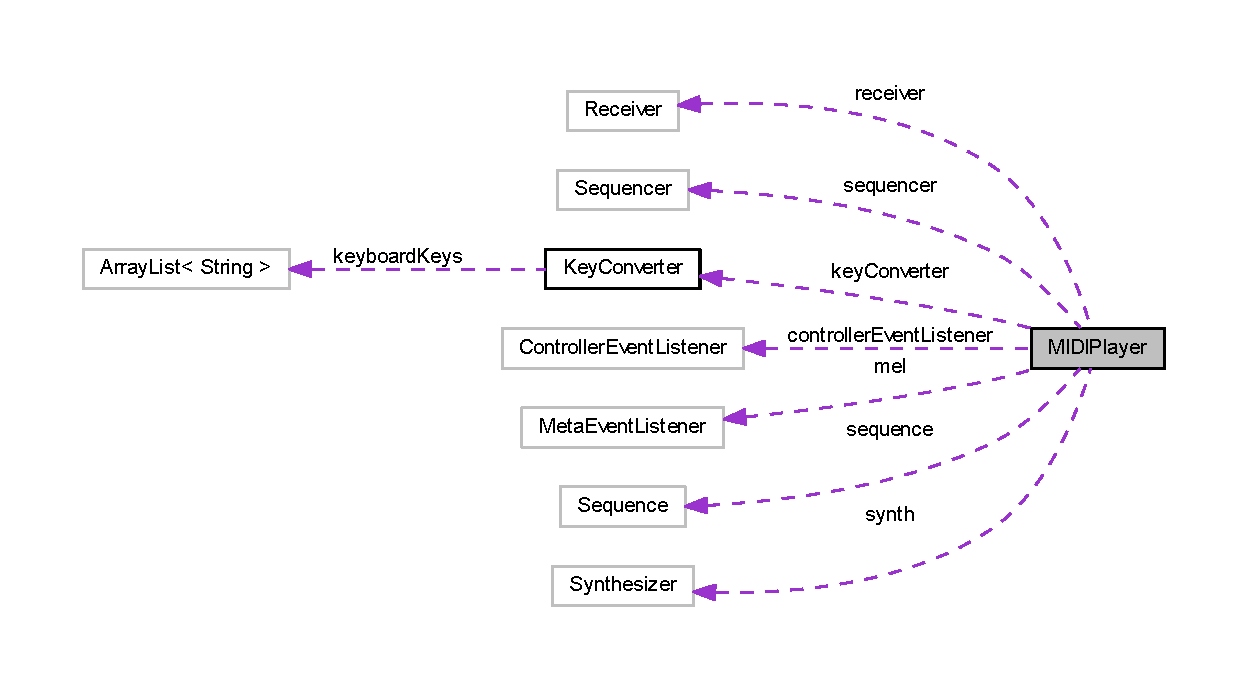
\includegraphics[width=350pt]{classcom_1_1lclion_1_1midiplayer_1_1_m_i_d_i_player__coll__graph}
\end{center}
\end{figure}
\subsection*{Public Member Functions}
\begin{DoxyCompactItemize}
\item 
\hyperlink{classcom_1_1lclion_1_1midiplayer_1_1_m_i_d_i_player_a0e4d3ba471e75a0430fbe278fcaa2888}{M\+I\+D\+I\+Player} (File file)
\item 
void \hyperlink{classcom_1_1lclion_1_1midiplayer_1_1_m_i_d_i_player_a28c694149ed3aa271b8dc56eb0785b96}{play\+Keys} (int\mbox{[}$\,$\mbox{]} keys)
\item 
void \hyperlink{classcom_1_1lclion_1_1midiplayer_1_1_m_i_d_i_player_a0bafa31e350020787d811f3697dceb86}{play\+M\+I\+D\+I} ()
\item 
void \hyperlink{classcom_1_1lclion_1_1midiplayer_1_1_m_i_d_i_player_a43e0304f725fff9064639507536d7203}{stop\+M\+I\+D\+I} ()
\item 
void \hyperlink{classcom_1_1lclion_1_1midiplayer_1_1_m_i_d_i_player_a0d9aa818aac57f70d4d9a27cb08aa68a}{pause\+M\+I\+D\+I} ()
\item 
void \hyperlink{classcom_1_1lclion_1_1midiplayer_1_1_m_i_d_i_player_ab82fe765a6f62ab63ed7f35c2c9b3002}{set\+Volume} (double \hyperlink{classcom_1_1lclion_1_1midiplayer_1_1_m_i_d_i_player_aed48ca0bcd2162fd4fd495873e2631f5}{volume})
\item 
void \hyperlink{classcom_1_1lclion_1_1midiplayer_1_1_m_i_d_i_player_a6f0d774251274a44de6466408b9d0193}{set\+Instrument} (int prog\+Num)
\item 
void \hyperlink{classcom_1_1lclion_1_1midiplayer_1_1_m_i_d_i_player_a5466c67c5ec22359c0702dc4ac8ffb19}{set\+Speed} (float speed)
\item 
void \hyperlink{classcom_1_1lclion_1_1midiplayer_1_1_m_i_d_i_player_a6d58098c6cf63c241ed03bc797256bb1}{play} ()
\item 
void \hyperlink{classcom_1_1lclion_1_1midiplayer_1_1_m_i_d_i_player_a7f758814eb3a4fc62794d0453b2cba42}{print\+Tick\+Pos} ()
\item 
boolean \hyperlink{classcom_1_1lclion_1_1midiplayer_1_1_m_i_d_i_player_a876c0699cfeae70f84fc508a4b05b6c0}{is\+Running} ()
\item 
void \hyperlink{classcom_1_1lclion_1_1midiplayer_1_1_m_i_d_i_player_adf42fe0a3253b9d6fed0dea0aba77cb4}{set\+Tick} (long tick)
\item 
long \hyperlink{classcom_1_1lclion_1_1midiplayer_1_1_m_i_d_i_player_a4e64895a61273ddd850ecdc7e7f1d639}{get\+Current\+Tick} ()
\item 
long \hyperlink{classcom_1_1lclion_1_1midiplayer_1_1_m_i_d_i_player_a318c504fc464b620e829b6ed354cc922}{get\+Tick\+Length} ()
\item 
Track\mbox{[}$\,$\mbox{]} \hyperlink{classcom_1_1lclion_1_1midiplayer_1_1_m_i_d_i_player_a9c00c1196a6593faccf3e71ee4ba7c84}{get\+Tracks} ()
\item 
void \hyperlink{classcom_1_1lclion_1_1midiplayer_1_1_m_i_d_i_player_a5ea586ca69152e093de72efaa30035ab}{mute\+Track} (int track\+Num)
\item 
void \hyperlink{classcom_1_1lclion_1_1midiplayer_1_1_m_i_d_i_player_a273586a96562827374d3167a6f844bf1}{unmute\+Track} (int track\+Num)
\item 
void \hyperlink{classcom_1_1lclion_1_1midiplayer_1_1_m_i_d_i_player_a32f4912c0d576586a49ecce3a41709e8}{unmute\+All\+Tracks} ()
\item 
void \hyperlink{classcom_1_1lclion_1_1midiplayer_1_1_m_i_d_i_player_a6b4104bceabf350464cc74e4d9babcb1}{print\+Patch\+List} ()
\end{DoxyCompactItemize}
\subsection*{Private Attributes}
\begin{DoxyCompactItemize}
\item 
int \hyperlink{classcom_1_1lclion_1_1midiplayer_1_1_m_i_d_i_player_adf7dff2c57c0da9a4a2b70e3e815be31}{channel} = 0
\item 
int \hyperlink{classcom_1_1lclion_1_1midiplayer_1_1_m_i_d_i_player_aed48ca0bcd2162fd4fd495873e2631f5}{volume} = 80
\item 
int \hyperlink{classcom_1_1lclion_1_1midiplayer_1_1_m_i_d_i_player_ac6e4b2a3cf932b33832d4e4e4e7cd0de}{duration} = 200
\item 
int \hyperlink{classcom_1_1lclion_1_1midiplayer_1_1_m_i_d_i_player_a421d9b518a4d3273cec866d51b135803}{current\+Instrument\+Patch\+Num} = -\/1
\item 
Sequence \hyperlink{classcom_1_1lclion_1_1midiplayer_1_1_m_i_d_i_player_aae9bd69432c806ce0c10016839a874a2}{sequence} = null
\item 
Sequencer \hyperlink{classcom_1_1lclion_1_1midiplayer_1_1_m_i_d_i_player_a857733a65a16f85598c03acd97305607}{sequencer} = null
\item 
Synthesizer \hyperlink{classcom_1_1lclion_1_1midiplayer_1_1_m_i_d_i_player_a4356e5541666df1f482a781ea4f6ff42}{synth}
\item 
\hyperlink{classcom_1_1lclion_1_1midiparser_1_1_key_converter}{Key\+Converter} \hyperlink{classcom_1_1lclion_1_1midiplayer_1_1_m_i_d_i_player_acc7c29517d4ac6fb6eb51b8d9b714728}{key\+Converter} = new \hyperlink{classcom_1_1lclion_1_1midiparser_1_1_key_converter}{Key\+Converter}()
\item 
String \hyperlink{classcom_1_1lclion_1_1midiplayer_1_1_m_i_d_i_player_af7f77ddd1de996adaa69c1f5d8492dfa}{text\+To\+Play} = null
\item 
Controller\+Event\+Listener \hyperlink{classcom_1_1lclion_1_1midiplayer_1_1_m_i_d_i_player_a3e129365b1af8a27e0e46ff8334d1415}{controller\+Event\+Listener} = null
\item 
Meta\+Event\+Listener \hyperlink{classcom_1_1lclion_1_1midiplayer_1_1_m_i_d_i_player_a4a46968d288601bb1f3180ee85507266}{mel} = null
\item 
Receiver \hyperlink{classcom_1_1lclion_1_1midiplayer_1_1_m_i_d_i_player_a679c25b0c10670fdd4d2fb4f8cd774ec}{receiver} = null
\end{DoxyCompactItemize}
\subsection*{Static Private Attributes}
\begin{DoxyCompactItemize}
\item 
static final int \hyperlink{classcom_1_1lclion_1_1midiplayer_1_1_m_i_d_i_player_ac035f42f6f27179d122b97d54fd030e1}{N\+O\+T\+E\+\_\+\+O\+N} = 0x90
\end{DoxyCompactItemize}


\subsection{Detailed Description}
A \hyperlink{classcom_1_1lclion_1_1midiplayer_1_1_m_i_d_i_player}{M\+I\+D\+I\+Player} that manages the playback of M\+I\+D\+I files. 

\begin{DoxyAuthor}{Author}
L\+C Lion 
\end{DoxyAuthor}


\subsection{Constructor \& Destructor Documentation}
\hypertarget{classcom_1_1lclion_1_1midiplayer_1_1_m_i_d_i_player_a0e4d3ba471e75a0430fbe278fcaa2888}{\index{com\+::lclion\+::midiplayer\+::\+M\+I\+D\+I\+Player@{com\+::lclion\+::midiplayer\+::\+M\+I\+D\+I\+Player}!M\+I\+D\+I\+Player@{M\+I\+D\+I\+Player}}
\index{M\+I\+D\+I\+Player@{M\+I\+D\+I\+Player}!com\+::lclion\+::midiplayer\+::\+M\+I\+D\+I\+Player@{com\+::lclion\+::midiplayer\+::\+M\+I\+D\+I\+Player}}
\subsubsection[{M\+I\+D\+I\+Player}]{\setlength{\rightskip}{0pt plus 5cm}{\bf M\+I\+D\+I\+Player} (
\begin{DoxyParamCaption}
\item[{File}]{file}
\end{DoxyParamCaption}
)}}\label{classcom_1_1lclion_1_1midiplayer_1_1_m_i_d_i_player_a0e4d3ba471e75a0430fbe278fcaa2888}


\subsection{Member Function Documentation}
\hypertarget{classcom_1_1lclion_1_1midiplayer_1_1_m_i_d_i_player_a4e64895a61273ddd850ecdc7e7f1d639}{\index{com\+::lclion\+::midiplayer\+::\+M\+I\+D\+I\+Player@{com\+::lclion\+::midiplayer\+::\+M\+I\+D\+I\+Player}!get\+Current\+Tick@{get\+Current\+Tick}}
\index{get\+Current\+Tick@{get\+Current\+Tick}!com\+::lclion\+::midiplayer\+::\+M\+I\+D\+I\+Player@{com\+::lclion\+::midiplayer\+::\+M\+I\+D\+I\+Player}}
\subsubsection[{get\+Current\+Tick}]{\setlength{\rightskip}{0pt plus 5cm}long get\+Current\+Tick (
\begin{DoxyParamCaption}
{}
\end{DoxyParamCaption}
)}}\label{classcom_1_1lclion_1_1midiplayer_1_1_m_i_d_i_player_a4e64895a61273ddd850ecdc7e7f1d639}
\hypertarget{classcom_1_1lclion_1_1midiplayer_1_1_m_i_d_i_player_a318c504fc464b620e829b6ed354cc922}{\index{com\+::lclion\+::midiplayer\+::\+M\+I\+D\+I\+Player@{com\+::lclion\+::midiplayer\+::\+M\+I\+D\+I\+Player}!get\+Tick\+Length@{get\+Tick\+Length}}
\index{get\+Tick\+Length@{get\+Tick\+Length}!com\+::lclion\+::midiplayer\+::\+M\+I\+D\+I\+Player@{com\+::lclion\+::midiplayer\+::\+M\+I\+D\+I\+Player}}
\subsubsection[{get\+Tick\+Length}]{\setlength{\rightskip}{0pt plus 5cm}long get\+Tick\+Length (
\begin{DoxyParamCaption}
{}
\end{DoxyParamCaption}
)}}\label{classcom_1_1lclion_1_1midiplayer_1_1_m_i_d_i_player_a318c504fc464b620e829b6ed354cc922}
\hypertarget{classcom_1_1lclion_1_1midiplayer_1_1_m_i_d_i_player_a9c00c1196a6593faccf3e71ee4ba7c84}{\index{com\+::lclion\+::midiplayer\+::\+M\+I\+D\+I\+Player@{com\+::lclion\+::midiplayer\+::\+M\+I\+D\+I\+Player}!get\+Tracks@{get\+Tracks}}
\index{get\+Tracks@{get\+Tracks}!com\+::lclion\+::midiplayer\+::\+M\+I\+D\+I\+Player@{com\+::lclion\+::midiplayer\+::\+M\+I\+D\+I\+Player}}
\subsubsection[{get\+Tracks}]{\setlength{\rightskip}{0pt plus 5cm}Track \mbox{[}$\,$\mbox{]} get\+Tracks (
\begin{DoxyParamCaption}
{}
\end{DoxyParamCaption}
)}}\label{classcom_1_1lclion_1_1midiplayer_1_1_m_i_d_i_player_a9c00c1196a6593faccf3e71ee4ba7c84}
\hypertarget{classcom_1_1lclion_1_1midiplayer_1_1_m_i_d_i_player_a876c0699cfeae70f84fc508a4b05b6c0}{\index{com\+::lclion\+::midiplayer\+::\+M\+I\+D\+I\+Player@{com\+::lclion\+::midiplayer\+::\+M\+I\+D\+I\+Player}!is\+Running@{is\+Running}}
\index{is\+Running@{is\+Running}!com\+::lclion\+::midiplayer\+::\+M\+I\+D\+I\+Player@{com\+::lclion\+::midiplayer\+::\+M\+I\+D\+I\+Player}}
\subsubsection[{is\+Running}]{\setlength{\rightskip}{0pt plus 5cm}boolean is\+Running (
\begin{DoxyParamCaption}
{}
\end{DoxyParamCaption}
)}}\label{classcom_1_1lclion_1_1midiplayer_1_1_m_i_d_i_player_a876c0699cfeae70f84fc508a4b05b6c0}
\hypertarget{classcom_1_1lclion_1_1midiplayer_1_1_m_i_d_i_player_a5ea586ca69152e093de72efaa30035ab}{\index{com\+::lclion\+::midiplayer\+::\+M\+I\+D\+I\+Player@{com\+::lclion\+::midiplayer\+::\+M\+I\+D\+I\+Player}!mute\+Track@{mute\+Track}}
\index{mute\+Track@{mute\+Track}!com\+::lclion\+::midiplayer\+::\+M\+I\+D\+I\+Player@{com\+::lclion\+::midiplayer\+::\+M\+I\+D\+I\+Player}}
\subsubsection[{mute\+Track}]{\setlength{\rightskip}{0pt plus 5cm}void mute\+Track (
\begin{DoxyParamCaption}
\item[{int}]{track\+Num}
\end{DoxyParamCaption}
)}}\label{classcom_1_1lclion_1_1midiplayer_1_1_m_i_d_i_player_a5ea586ca69152e093de72efaa30035ab}
\hypertarget{classcom_1_1lclion_1_1midiplayer_1_1_m_i_d_i_player_a0d9aa818aac57f70d4d9a27cb08aa68a}{\index{com\+::lclion\+::midiplayer\+::\+M\+I\+D\+I\+Player@{com\+::lclion\+::midiplayer\+::\+M\+I\+D\+I\+Player}!pause\+M\+I\+D\+I@{pause\+M\+I\+D\+I}}
\index{pause\+M\+I\+D\+I@{pause\+M\+I\+D\+I}!com\+::lclion\+::midiplayer\+::\+M\+I\+D\+I\+Player@{com\+::lclion\+::midiplayer\+::\+M\+I\+D\+I\+Player}}
\subsubsection[{pause\+M\+I\+D\+I}]{\setlength{\rightskip}{0pt plus 5cm}void pause\+M\+I\+D\+I (
\begin{DoxyParamCaption}
{}
\end{DoxyParamCaption}
)}}\label{classcom_1_1lclion_1_1midiplayer_1_1_m_i_d_i_player_a0d9aa818aac57f70d4d9a27cb08aa68a}
\hypertarget{classcom_1_1lclion_1_1midiplayer_1_1_m_i_d_i_player_a6d58098c6cf63c241ed03bc797256bb1}{\index{com\+::lclion\+::midiplayer\+::\+M\+I\+D\+I\+Player@{com\+::lclion\+::midiplayer\+::\+M\+I\+D\+I\+Player}!play@{play}}
\index{play@{play}!com\+::lclion\+::midiplayer\+::\+M\+I\+D\+I\+Player@{com\+::lclion\+::midiplayer\+::\+M\+I\+D\+I\+Player}}
\subsubsection[{play}]{\setlength{\rightskip}{0pt plus 5cm}void play (
\begin{DoxyParamCaption}
{}
\end{DoxyParamCaption}
)}}\label{classcom_1_1lclion_1_1midiplayer_1_1_m_i_d_i_player_a6d58098c6cf63c241ed03bc797256bb1}
\hypertarget{classcom_1_1lclion_1_1midiplayer_1_1_m_i_d_i_player_a28c694149ed3aa271b8dc56eb0785b96}{\index{com\+::lclion\+::midiplayer\+::\+M\+I\+D\+I\+Player@{com\+::lclion\+::midiplayer\+::\+M\+I\+D\+I\+Player}!play\+Keys@{play\+Keys}}
\index{play\+Keys@{play\+Keys}!com\+::lclion\+::midiplayer\+::\+M\+I\+D\+I\+Player@{com\+::lclion\+::midiplayer\+::\+M\+I\+D\+I\+Player}}
\subsubsection[{play\+Keys}]{\setlength{\rightskip}{0pt plus 5cm}void play\+Keys (
\begin{DoxyParamCaption}
\item[{int\mbox{[}$\,$\mbox{]}}]{keys}
\end{DoxyParamCaption}
)}}\label{classcom_1_1lclion_1_1midiplayer_1_1_m_i_d_i_player_a28c694149ed3aa271b8dc56eb0785b96}
\hypertarget{classcom_1_1lclion_1_1midiplayer_1_1_m_i_d_i_player_a0bafa31e350020787d811f3697dceb86}{\index{com\+::lclion\+::midiplayer\+::\+M\+I\+D\+I\+Player@{com\+::lclion\+::midiplayer\+::\+M\+I\+D\+I\+Player}!play\+M\+I\+D\+I@{play\+M\+I\+D\+I}}
\index{play\+M\+I\+D\+I@{play\+M\+I\+D\+I}!com\+::lclion\+::midiplayer\+::\+M\+I\+D\+I\+Player@{com\+::lclion\+::midiplayer\+::\+M\+I\+D\+I\+Player}}
\subsubsection[{play\+M\+I\+D\+I}]{\setlength{\rightskip}{0pt plus 5cm}void play\+M\+I\+D\+I (
\begin{DoxyParamCaption}
{}
\end{DoxyParamCaption}
)}}\label{classcom_1_1lclion_1_1midiplayer_1_1_m_i_d_i_player_a0bafa31e350020787d811f3697dceb86}


Here is the call graph for this function\+:\nopagebreak
\begin{figure}[H]
\begin{center}
\leavevmode
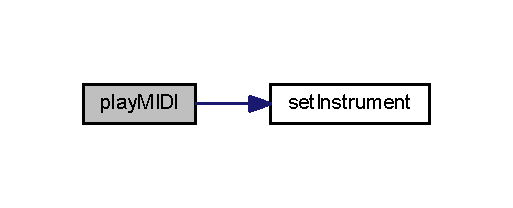
\includegraphics[width=246pt]{classcom_1_1lclion_1_1midiplayer_1_1_m_i_d_i_player_a0bafa31e350020787d811f3697dceb86_cgraph}
\end{center}
\end{figure}


\hypertarget{classcom_1_1lclion_1_1midiplayer_1_1_m_i_d_i_player_a6b4104bceabf350464cc74e4d9babcb1}{\index{com\+::lclion\+::midiplayer\+::\+M\+I\+D\+I\+Player@{com\+::lclion\+::midiplayer\+::\+M\+I\+D\+I\+Player}!print\+Patch\+List@{print\+Patch\+List}}
\index{print\+Patch\+List@{print\+Patch\+List}!com\+::lclion\+::midiplayer\+::\+M\+I\+D\+I\+Player@{com\+::lclion\+::midiplayer\+::\+M\+I\+D\+I\+Player}}
\subsubsection[{print\+Patch\+List}]{\setlength{\rightskip}{0pt plus 5cm}void print\+Patch\+List (
\begin{DoxyParamCaption}
{}
\end{DoxyParamCaption}
)}}\label{classcom_1_1lclion_1_1midiplayer_1_1_m_i_d_i_player_a6b4104bceabf350464cc74e4d9babcb1}
\hypertarget{classcom_1_1lclion_1_1midiplayer_1_1_m_i_d_i_player_a7f758814eb3a4fc62794d0453b2cba42}{\index{com\+::lclion\+::midiplayer\+::\+M\+I\+D\+I\+Player@{com\+::lclion\+::midiplayer\+::\+M\+I\+D\+I\+Player}!print\+Tick\+Pos@{print\+Tick\+Pos}}
\index{print\+Tick\+Pos@{print\+Tick\+Pos}!com\+::lclion\+::midiplayer\+::\+M\+I\+D\+I\+Player@{com\+::lclion\+::midiplayer\+::\+M\+I\+D\+I\+Player}}
\subsubsection[{print\+Tick\+Pos}]{\setlength{\rightskip}{0pt plus 5cm}void print\+Tick\+Pos (
\begin{DoxyParamCaption}
{}
\end{DoxyParamCaption}
)}}\label{classcom_1_1lclion_1_1midiplayer_1_1_m_i_d_i_player_a7f758814eb3a4fc62794d0453b2cba42}
\hypertarget{classcom_1_1lclion_1_1midiplayer_1_1_m_i_d_i_player_a6f0d774251274a44de6466408b9d0193}{\index{com\+::lclion\+::midiplayer\+::\+M\+I\+D\+I\+Player@{com\+::lclion\+::midiplayer\+::\+M\+I\+D\+I\+Player}!set\+Instrument@{set\+Instrument}}
\index{set\+Instrument@{set\+Instrument}!com\+::lclion\+::midiplayer\+::\+M\+I\+D\+I\+Player@{com\+::lclion\+::midiplayer\+::\+M\+I\+D\+I\+Player}}
\subsubsection[{set\+Instrument}]{\setlength{\rightskip}{0pt plus 5cm}void set\+Instrument (
\begin{DoxyParamCaption}
\item[{int}]{prog\+Num}
\end{DoxyParamCaption}
)}}\label{classcom_1_1lclion_1_1midiplayer_1_1_m_i_d_i_player_a6f0d774251274a44de6466408b9d0193}
\hypertarget{classcom_1_1lclion_1_1midiplayer_1_1_m_i_d_i_player_a5466c67c5ec22359c0702dc4ac8ffb19}{\index{com\+::lclion\+::midiplayer\+::\+M\+I\+D\+I\+Player@{com\+::lclion\+::midiplayer\+::\+M\+I\+D\+I\+Player}!set\+Speed@{set\+Speed}}
\index{set\+Speed@{set\+Speed}!com\+::lclion\+::midiplayer\+::\+M\+I\+D\+I\+Player@{com\+::lclion\+::midiplayer\+::\+M\+I\+D\+I\+Player}}
\subsubsection[{set\+Speed}]{\setlength{\rightskip}{0pt plus 5cm}void set\+Speed (
\begin{DoxyParamCaption}
\item[{float}]{speed}
\end{DoxyParamCaption}
)}}\label{classcom_1_1lclion_1_1midiplayer_1_1_m_i_d_i_player_a5466c67c5ec22359c0702dc4ac8ffb19}
\hypertarget{classcom_1_1lclion_1_1midiplayer_1_1_m_i_d_i_player_adf42fe0a3253b9d6fed0dea0aba77cb4}{\index{com\+::lclion\+::midiplayer\+::\+M\+I\+D\+I\+Player@{com\+::lclion\+::midiplayer\+::\+M\+I\+D\+I\+Player}!set\+Tick@{set\+Tick}}
\index{set\+Tick@{set\+Tick}!com\+::lclion\+::midiplayer\+::\+M\+I\+D\+I\+Player@{com\+::lclion\+::midiplayer\+::\+M\+I\+D\+I\+Player}}
\subsubsection[{set\+Tick}]{\setlength{\rightskip}{0pt plus 5cm}void set\+Tick (
\begin{DoxyParamCaption}
\item[{long}]{tick}
\end{DoxyParamCaption}
)}}\label{classcom_1_1lclion_1_1midiplayer_1_1_m_i_d_i_player_adf42fe0a3253b9d6fed0dea0aba77cb4}
\hypertarget{classcom_1_1lclion_1_1midiplayer_1_1_m_i_d_i_player_ab82fe765a6f62ab63ed7f35c2c9b3002}{\index{com\+::lclion\+::midiplayer\+::\+M\+I\+D\+I\+Player@{com\+::lclion\+::midiplayer\+::\+M\+I\+D\+I\+Player}!set\+Volume@{set\+Volume}}
\index{set\+Volume@{set\+Volume}!com\+::lclion\+::midiplayer\+::\+M\+I\+D\+I\+Player@{com\+::lclion\+::midiplayer\+::\+M\+I\+D\+I\+Player}}
\subsubsection[{set\+Volume}]{\setlength{\rightskip}{0pt plus 5cm}void set\+Volume (
\begin{DoxyParamCaption}
\item[{double}]{volume}
\end{DoxyParamCaption}
)}}\label{classcom_1_1lclion_1_1midiplayer_1_1_m_i_d_i_player_ab82fe765a6f62ab63ed7f35c2c9b3002}
\hypertarget{classcom_1_1lclion_1_1midiplayer_1_1_m_i_d_i_player_a43e0304f725fff9064639507536d7203}{\index{com\+::lclion\+::midiplayer\+::\+M\+I\+D\+I\+Player@{com\+::lclion\+::midiplayer\+::\+M\+I\+D\+I\+Player}!stop\+M\+I\+D\+I@{stop\+M\+I\+D\+I}}
\index{stop\+M\+I\+D\+I@{stop\+M\+I\+D\+I}!com\+::lclion\+::midiplayer\+::\+M\+I\+D\+I\+Player@{com\+::lclion\+::midiplayer\+::\+M\+I\+D\+I\+Player}}
\subsubsection[{stop\+M\+I\+D\+I}]{\setlength{\rightskip}{0pt plus 5cm}void stop\+M\+I\+D\+I (
\begin{DoxyParamCaption}
{}
\end{DoxyParamCaption}
)}}\label{classcom_1_1lclion_1_1midiplayer_1_1_m_i_d_i_player_a43e0304f725fff9064639507536d7203}
\hypertarget{classcom_1_1lclion_1_1midiplayer_1_1_m_i_d_i_player_a32f4912c0d576586a49ecce3a41709e8}{\index{com\+::lclion\+::midiplayer\+::\+M\+I\+D\+I\+Player@{com\+::lclion\+::midiplayer\+::\+M\+I\+D\+I\+Player}!unmute\+All\+Tracks@{unmute\+All\+Tracks}}
\index{unmute\+All\+Tracks@{unmute\+All\+Tracks}!com\+::lclion\+::midiplayer\+::\+M\+I\+D\+I\+Player@{com\+::lclion\+::midiplayer\+::\+M\+I\+D\+I\+Player}}
\subsubsection[{unmute\+All\+Tracks}]{\setlength{\rightskip}{0pt plus 5cm}void unmute\+All\+Tracks (
\begin{DoxyParamCaption}
{}
\end{DoxyParamCaption}
)}}\label{classcom_1_1lclion_1_1midiplayer_1_1_m_i_d_i_player_a32f4912c0d576586a49ecce3a41709e8}
\hypertarget{classcom_1_1lclion_1_1midiplayer_1_1_m_i_d_i_player_a273586a96562827374d3167a6f844bf1}{\index{com\+::lclion\+::midiplayer\+::\+M\+I\+D\+I\+Player@{com\+::lclion\+::midiplayer\+::\+M\+I\+D\+I\+Player}!unmute\+Track@{unmute\+Track}}
\index{unmute\+Track@{unmute\+Track}!com\+::lclion\+::midiplayer\+::\+M\+I\+D\+I\+Player@{com\+::lclion\+::midiplayer\+::\+M\+I\+D\+I\+Player}}
\subsubsection[{unmute\+Track}]{\setlength{\rightskip}{0pt plus 5cm}void unmute\+Track (
\begin{DoxyParamCaption}
\item[{int}]{track\+Num}
\end{DoxyParamCaption}
)}}\label{classcom_1_1lclion_1_1midiplayer_1_1_m_i_d_i_player_a273586a96562827374d3167a6f844bf1}


\subsection{Member Data Documentation}
\hypertarget{classcom_1_1lclion_1_1midiplayer_1_1_m_i_d_i_player_adf7dff2c57c0da9a4a2b70e3e815be31}{\index{com\+::lclion\+::midiplayer\+::\+M\+I\+D\+I\+Player@{com\+::lclion\+::midiplayer\+::\+M\+I\+D\+I\+Player}!channel@{channel}}
\index{channel@{channel}!com\+::lclion\+::midiplayer\+::\+M\+I\+D\+I\+Player@{com\+::lclion\+::midiplayer\+::\+M\+I\+D\+I\+Player}}
\subsubsection[{channel}]{\setlength{\rightskip}{0pt plus 5cm}int channel = 0\hspace{0.3cm}{\ttfamily [private]}}}\label{classcom_1_1lclion_1_1midiplayer_1_1_m_i_d_i_player_adf7dff2c57c0da9a4a2b70e3e815be31}
\hypertarget{classcom_1_1lclion_1_1midiplayer_1_1_m_i_d_i_player_a3e129365b1af8a27e0e46ff8334d1415}{\index{com\+::lclion\+::midiplayer\+::\+M\+I\+D\+I\+Player@{com\+::lclion\+::midiplayer\+::\+M\+I\+D\+I\+Player}!controller\+Event\+Listener@{controller\+Event\+Listener}}
\index{controller\+Event\+Listener@{controller\+Event\+Listener}!com\+::lclion\+::midiplayer\+::\+M\+I\+D\+I\+Player@{com\+::lclion\+::midiplayer\+::\+M\+I\+D\+I\+Player}}
\subsubsection[{controller\+Event\+Listener}]{\setlength{\rightskip}{0pt plus 5cm}Controller\+Event\+Listener controller\+Event\+Listener = null\hspace{0.3cm}{\ttfamily [private]}}}\label{classcom_1_1lclion_1_1midiplayer_1_1_m_i_d_i_player_a3e129365b1af8a27e0e46ff8334d1415}
\hypertarget{classcom_1_1lclion_1_1midiplayer_1_1_m_i_d_i_player_a421d9b518a4d3273cec866d51b135803}{\index{com\+::lclion\+::midiplayer\+::\+M\+I\+D\+I\+Player@{com\+::lclion\+::midiplayer\+::\+M\+I\+D\+I\+Player}!current\+Instrument\+Patch\+Num@{current\+Instrument\+Patch\+Num}}
\index{current\+Instrument\+Patch\+Num@{current\+Instrument\+Patch\+Num}!com\+::lclion\+::midiplayer\+::\+M\+I\+D\+I\+Player@{com\+::lclion\+::midiplayer\+::\+M\+I\+D\+I\+Player}}
\subsubsection[{current\+Instrument\+Patch\+Num}]{\setlength{\rightskip}{0pt plus 5cm}int current\+Instrument\+Patch\+Num = -\/1\hspace{0.3cm}{\ttfamily [private]}}}\label{classcom_1_1lclion_1_1midiplayer_1_1_m_i_d_i_player_a421d9b518a4d3273cec866d51b135803}
\hypertarget{classcom_1_1lclion_1_1midiplayer_1_1_m_i_d_i_player_ac6e4b2a3cf932b33832d4e4e4e7cd0de}{\index{com\+::lclion\+::midiplayer\+::\+M\+I\+D\+I\+Player@{com\+::lclion\+::midiplayer\+::\+M\+I\+D\+I\+Player}!duration@{duration}}
\index{duration@{duration}!com\+::lclion\+::midiplayer\+::\+M\+I\+D\+I\+Player@{com\+::lclion\+::midiplayer\+::\+M\+I\+D\+I\+Player}}
\subsubsection[{duration}]{\setlength{\rightskip}{0pt plus 5cm}int duration = 200\hspace{0.3cm}{\ttfamily [private]}}}\label{classcom_1_1lclion_1_1midiplayer_1_1_m_i_d_i_player_ac6e4b2a3cf932b33832d4e4e4e7cd0de}
\hypertarget{classcom_1_1lclion_1_1midiplayer_1_1_m_i_d_i_player_acc7c29517d4ac6fb6eb51b8d9b714728}{\index{com\+::lclion\+::midiplayer\+::\+M\+I\+D\+I\+Player@{com\+::lclion\+::midiplayer\+::\+M\+I\+D\+I\+Player}!key\+Converter@{key\+Converter}}
\index{key\+Converter@{key\+Converter}!com\+::lclion\+::midiplayer\+::\+M\+I\+D\+I\+Player@{com\+::lclion\+::midiplayer\+::\+M\+I\+D\+I\+Player}}
\subsubsection[{key\+Converter}]{\setlength{\rightskip}{0pt plus 5cm}{\bf Key\+Converter} key\+Converter = new {\bf Key\+Converter}()\hspace{0.3cm}{\ttfamily [private]}}}\label{classcom_1_1lclion_1_1midiplayer_1_1_m_i_d_i_player_acc7c29517d4ac6fb6eb51b8d9b714728}
\hypertarget{classcom_1_1lclion_1_1midiplayer_1_1_m_i_d_i_player_a4a46968d288601bb1f3180ee85507266}{\index{com\+::lclion\+::midiplayer\+::\+M\+I\+D\+I\+Player@{com\+::lclion\+::midiplayer\+::\+M\+I\+D\+I\+Player}!mel@{mel}}
\index{mel@{mel}!com\+::lclion\+::midiplayer\+::\+M\+I\+D\+I\+Player@{com\+::lclion\+::midiplayer\+::\+M\+I\+D\+I\+Player}}
\subsubsection[{mel}]{\setlength{\rightskip}{0pt plus 5cm}Meta\+Event\+Listener mel = null\hspace{0.3cm}{\ttfamily [private]}}}\label{classcom_1_1lclion_1_1midiplayer_1_1_m_i_d_i_player_a4a46968d288601bb1f3180ee85507266}
\hypertarget{classcom_1_1lclion_1_1midiplayer_1_1_m_i_d_i_player_ac035f42f6f27179d122b97d54fd030e1}{\index{com\+::lclion\+::midiplayer\+::\+M\+I\+D\+I\+Player@{com\+::lclion\+::midiplayer\+::\+M\+I\+D\+I\+Player}!N\+O\+T\+E\+\_\+\+O\+N@{N\+O\+T\+E\+\_\+\+O\+N}}
\index{N\+O\+T\+E\+\_\+\+O\+N@{N\+O\+T\+E\+\_\+\+O\+N}!com\+::lclion\+::midiplayer\+::\+M\+I\+D\+I\+Player@{com\+::lclion\+::midiplayer\+::\+M\+I\+D\+I\+Player}}
\subsubsection[{N\+O\+T\+E\+\_\+\+O\+N}]{\setlength{\rightskip}{0pt plus 5cm}final int N\+O\+T\+E\+\_\+\+O\+N = 0x90\hspace{0.3cm}{\ttfamily [static]}, {\ttfamily [private]}}}\label{classcom_1_1lclion_1_1midiplayer_1_1_m_i_d_i_player_ac035f42f6f27179d122b97d54fd030e1}
\hypertarget{classcom_1_1lclion_1_1midiplayer_1_1_m_i_d_i_player_a679c25b0c10670fdd4d2fb4f8cd774ec}{\index{com\+::lclion\+::midiplayer\+::\+M\+I\+D\+I\+Player@{com\+::lclion\+::midiplayer\+::\+M\+I\+D\+I\+Player}!receiver@{receiver}}
\index{receiver@{receiver}!com\+::lclion\+::midiplayer\+::\+M\+I\+D\+I\+Player@{com\+::lclion\+::midiplayer\+::\+M\+I\+D\+I\+Player}}
\subsubsection[{receiver}]{\setlength{\rightskip}{0pt plus 5cm}Receiver receiver = null\hspace{0.3cm}{\ttfamily [private]}}}\label{classcom_1_1lclion_1_1midiplayer_1_1_m_i_d_i_player_a679c25b0c10670fdd4d2fb4f8cd774ec}
\hypertarget{classcom_1_1lclion_1_1midiplayer_1_1_m_i_d_i_player_aae9bd69432c806ce0c10016839a874a2}{\index{com\+::lclion\+::midiplayer\+::\+M\+I\+D\+I\+Player@{com\+::lclion\+::midiplayer\+::\+M\+I\+D\+I\+Player}!sequence@{sequence}}
\index{sequence@{sequence}!com\+::lclion\+::midiplayer\+::\+M\+I\+D\+I\+Player@{com\+::lclion\+::midiplayer\+::\+M\+I\+D\+I\+Player}}
\subsubsection[{sequence}]{\setlength{\rightskip}{0pt plus 5cm}Sequence sequence = null\hspace{0.3cm}{\ttfamily [private]}}}\label{classcom_1_1lclion_1_1midiplayer_1_1_m_i_d_i_player_aae9bd69432c806ce0c10016839a874a2}
\hypertarget{classcom_1_1lclion_1_1midiplayer_1_1_m_i_d_i_player_a857733a65a16f85598c03acd97305607}{\index{com\+::lclion\+::midiplayer\+::\+M\+I\+D\+I\+Player@{com\+::lclion\+::midiplayer\+::\+M\+I\+D\+I\+Player}!sequencer@{sequencer}}
\index{sequencer@{sequencer}!com\+::lclion\+::midiplayer\+::\+M\+I\+D\+I\+Player@{com\+::lclion\+::midiplayer\+::\+M\+I\+D\+I\+Player}}
\subsubsection[{sequencer}]{\setlength{\rightskip}{0pt plus 5cm}Sequencer sequencer = null\hspace{0.3cm}{\ttfamily [private]}}}\label{classcom_1_1lclion_1_1midiplayer_1_1_m_i_d_i_player_a857733a65a16f85598c03acd97305607}
\hypertarget{classcom_1_1lclion_1_1midiplayer_1_1_m_i_d_i_player_a4356e5541666df1f482a781ea4f6ff42}{\index{com\+::lclion\+::midiplayer\+::\+M\+I\+D\+I\+Player@{com\+::lclion\+::midiplayer\+::\+M\+I\+D\+I\+Player}!synth@{synth}}
\index{synth@{synth}!com\+::lclion\+::midiplayer\+::\+M\+I\+D\+I\+Player@{com\+::lclion\+::midiplayer\+::\+M\+I\+D\+I\+Player}}
\subsubsection[{synth}]{\setlength{\rightskip}{0pt plus 5cm}Synthesizer synth\hspace{0.3cm}{\ttfamily [private]}}}\label{classcom_1_1lclion_1_1midiplayer_1_1_m_i_d_i_player_a4356e5541666df1f482a781ea4f6ff42}
\hypertarget{classcom_1_1lclion_1_1midiplayer_1_1_m_i_d_i_player_af7f77ddd1de996adaa69c1f5d8492dfa}{\index{com\+::lclion\+::midiplayer\+::\+M\+I\+D\+I\+Player@{com\+::lclion\+::midiplayer\+::\+M\+I\+D\+I\+Player}!text\+To\+Play@{text\+To\+Play}}
\index{text\+To\+Play@{text\+To\+Play}!com\+::lclion\+::midiplayer\+::\+M\+I\+D\+I\+Player@{com\+::lclion\+::midiplayer\+::\+M\+I\+D\+I\+Player}}
\subsubsection[{text\+To\+Play}]{\setlength{\rightskip}{0pt plus 5cm}String text\+To\+Play = null\hspace{0.3cm}{\ttfamily [private]}}}\label{classcom_1_1lclion_1_1midiplayer_1_1_m_i_d_i_player_af7f77ddd1de996adaa69c1f5d8492dfa}
\hypertarget{classcom_1_1lclion_1_1midiplayer_1_1_m_i_d_i_player_aed48ca0bcd2162fd4fd495873e2631f5}{\index{com\+::lclion\+::midiplayer\+::\+M\+I\+D\+I\+Player@{com\+::lclion\+::midiplayer\+::\+M\+I\+D\+I\+Player}!volume@{volume}}
\index{volume@{volume}!com\+::lclion\+::midiplayer\+::\+M\+I\+D\+I\+Player@{com\+::lclion\+::midiplayer\+::\+M\+I\+D\+I\+Player}}
\subsubsection[{volume}]{\setlength{\rightskip}{0pt plus 5cm}int volume = 80\hspace{0.3cm}{\ttfamily [private]}}}\label{classcom_1_1lclion_1_1midiplayer_1_1_m_i_d_i_player_aed48ca0bcd2162fd4fd495873e2631f5}


The documentation for this class was generated from the following file\+:\begin{DoxyCompactItemize}
\item 
src/com/lclion/midiplayer/\hyperlink{_m_i_d_i_player_8java}{M\+I\+D\+I\+Player.\+java}\end{DoxyCompactItemize}

\hypertarget{classcom_1_1lclion_1_1midiparser_1_1_note_colour_converter}{\section{Note\+Colour\+Converter Class Reference}
\label{classcom_1_1lclion_1_1midiparser_1_1_note_colour_converter}\index{Note\+Colour\+Converter@{Note\+Colour\+Converter}}
}


Uses style documents to colourise its corresponding note values into colours.  




Collaboration diagram for Note\+Colour\+Converter\+:\nopagebreak
\begin{figure}[H]
\begin{center}
\leavevmode
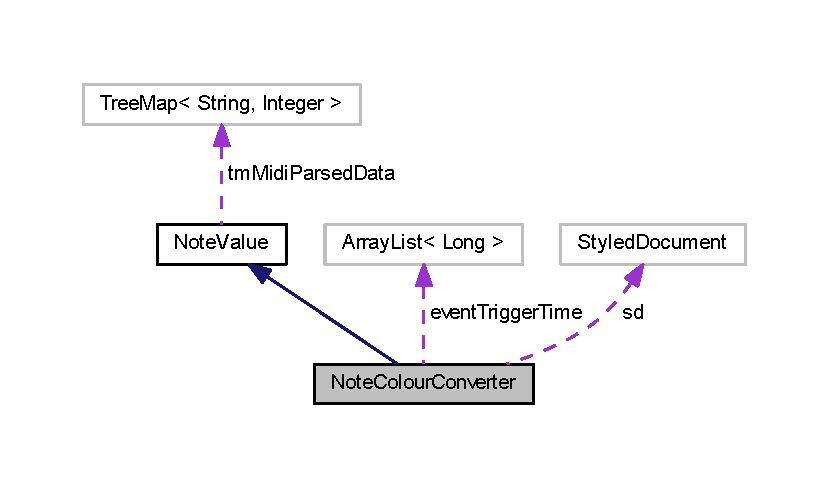
\includegraphics[width=350pt]{classcom_1_1lclion_1_1midiparser_1_1_note_colour_converter__coll__graph}
\end{center}
\end{figure}
\subsection*{Public Member Functions}
\begin{DoxyCompactItemize}
\item 
\hyperlink{classcom_1_1lclion_1_1midiparser_1_1_note_colour_converter_a63a6286bf21baa00408e9c77f8959374}{Note\+Colour\+Converter} (Styled\+Document \hyperlink{classcom_1_1lclion_1_1midiparser_1_1_note_colour_converter_ac31cda90c1001f063265ba84725dd62e}{sd}, Array\+List$<$ Long $>$ \hyperlink{classcom_1_1lclion_1_1midiparser_1_1_note_colour_converter_a74fa4197a892bf1767a6e5eb295e00ab}{event\+Trigger\+Time}, int \hyperlink{classcom_1_1lclion_1_1midiparser_1_1_note_colour_converter_a52304efcbc33b0b7cb2b3db90a30cc6d}{quarter\+Note})
\item 
Styled\+Document \hyperlink{classcom_1_1lclion_1_1midiparser_1_1_note_colour_converter_a1182e71888040b74469d2a6329c0e363}{Colourise\+Notes} ()
\end{DoxyCompactItemize}
\subsection*{Package Attributes}
\begin{DoxyCompactItemize}
\item 
Styled\+Document \hyperlink{classcom_1_1lclion_1_1midiparser_1_1_note_colour_converter_ac31cda90c1001f063265ba84725dd62e}{sd} = null
\item 
Array\+List$<$ Long $>$ \hyperlink{classcom_1_1lclion_1_1midiparser_1_1_note_colour_converter_a74fa4197a892bf1767a6e5eb295e00ab}{event\+Trigger\+Time} = null
\item 
int \hyperlink{classcom_1_1lclion_1_1midiparser_1_1_note_colour_converter_a52304efcbc33b0b7cb2b3db90a30cc6d}{quarter\+Note} = 0
\end{DoxyCompactItemize}
\subsection*{Additional Inherited Members}


\subsection{Detailed Description}
Uses style documents to colourise its corresponding note values into colours. 

\begin{DoxyAuthor}{Author}
L\+C Lion 
\end{DoxyAuthor}


\subsection{Constructor \& Destructor Documentation}
\hypertarget{classcom_1_1lclion_1_1midiparser_1_1_note_colour_converter_a63a6286bf21baa00408e9c77f8959374}{\index{com\+::lclion\+::midiparser\+::\+Note\+Colour\+Converter@{com\+::lclion\+::midiparser\+::\+Note\+Colour\+Converter}!Note\+Colour\+Converter@{Note\+Colour\+Converter}}
\index{Note\+Colour\+Converter@{Note\+Colour\+Converter}!com\+::lclion\+::midiparser\+::\+Note\+Colour\+Converter@{com\+::lclion\+::midiparser\+::\+Note\+Colour\+Converter}}
\subsubsection[{Note\+Colour\+Converter}]{\setlength{\rightskip}{0pt plus 5cm}{\bf Note\+Colour\+Converter} (
\begin{DoxyParamCaption}
\item[{Styled\+Document}]{sd, }
\item[{Array\+List$<$ Long $>$}]{event\+Trigger\+Time, }
\item[{int}]{quarter\+Note}
\end{DoxyParamCaption}
)}}\label{classcom_1_1lclion_1_1midiparser_1_1_note_colour_converter_a63a6286bf21baa00408e9c77f8959374}


Here is the call graph for this function\+:\nopagebreak
\begin{figure}[H]
\begin{center}
\leavevmode
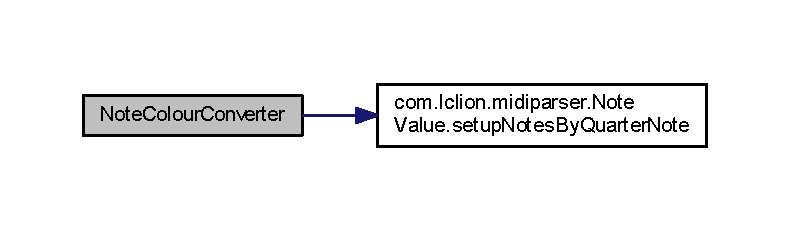
\includegraphics[width=350pt]{classcom_1_1lclion_1_1midiparser_1_1_note_colour_converter_a63a6286bf21baa00408e9c77f8959374_cgraph}
\end{center}
\end{figure}




\subsection{Member Function Documentation}
\hypertarget{classcom_1_1lclion_1_1midiparser_1_1_note_colour_converter_a1182e71888040b74469d2a6329c0e363}{\index{com\+::lclion\+::midiparser\+::\+Note\+Colour\+Converter@{com\+::lclion\+::midiparser\+::\+Note\+Colour\+Converter}!Colourise\+Notes@{Colourise\+Notes}}
\index{Colourise\+Notes@{Colourise\+Notes}!com\+::lclion\+::midiparser\+::\+Note\+Colour\+Converter@{com\+::lclion\+::midiparser\+::\+Note\+Colour\+Converter}}
\subsubsection[{Colourise\+Notes}]{\setlength{\rightskip}{0pt plus 5cm}Styled\+Document Colourise\+Notes (
\begin{DoxyParamCaption}
{}
\end{DoxyParamCaption}
)}}\label{classcom_1_1lclion_1_1midiparser_1_1_note_colour_converter_a1182e71888040b74469d2a6329c0e363}


\subsection{Member Data Documentation}
\hypertarget{classcom_1_1lclion_1_1midiparser_1_1_note_colour_converter_a74fa4197a892bf1767a6e5eb295e00ab}{\index{com\+::lclion\+::midiparser\+::\+Note\+Colour\+Converter@{com\+::lclion\+::midiparser\+::\+Note\+Colour\+Converter}!event\+Trigger\+Time@{event\+Trigger\+Time}}
\index{event\+Trigger\+Time@{event\+Trigger\+Time}!com\+::lclion\+::midiparser\+::\+Note\+Colour\+Converter@{com\+::lclion\+::midiparser\+::\+Note\+Colour\+Converter}}
\subsubsection[{event\+Trigger\+Time}]{\setlength{\rightskip}{0pt plus 5cm}Array\+List$<$Long$>$ event\+Trigger\+Time = null\hspace{0.3cm}{\ttfamily [package]}}}\label{classcom_1_1lclion_1_1midiparser_1_1_note_colour_converter_a74fa4197a892bf1767a6e5eb295e00ab}
\hypertarget{classcom_1_1lclion_1_1midiparser_1_1_note_colour_converter_a52304efcbc33b0b7cb2b3db90a30cc6d}{\index{com\+::lclion\+::midiparser\+::\+Note\+Colour\+Converter@{com\+::lclion\+::midiparser\+::\+Note\+Colour\+Converter}!quarter\+Note@{quarter\+Note}}
\index{quarter\+Note@{quarter\+Note}!com\+::lclion\+::midiparser\+::\+Note\+Colour\+Converter@{com\+::lclion\+::midiparser\+::\+Note\+Colour\+Converter}}
\subsubsection[{quarter\+Note}]{\setlength{\rightskip}{0pt plus 5cm}int quarter\+Note = 0\hspace{0.3cm}{\ttfamily [package]}}}\label{classcom_1_1lclion_1_1midiparser_1_1_note_colour_converter_a52304efcbc33b0b7cb2b3db90a30cc6d}
\hypertarget{classcom_1_1lclion_1_1midiparser_1_1_note_colour_converter_ac31cda90c1001f063265ba84725dd62e}{\index{com\+::lclion\+::midiparser\+::\+Note\+Colour\+Converter@{com\+::lclion\+::midiparser\+::\+Note\+Colour\+Converter}!sd@{sd}}
\index{sd@{sd}!com\+::lclion\+::midiparser\+::\+Note\+Colour\+Converter@{com\+::lclion\+::midiparser\+::\+Note\+Colour\+Converter}}
\subsubsection[{sd}]{\setlength{\rightskip}{0pt plus 5cm}Styled\+Document sd = null\hspace{0.3cm}{\ttfamily [package]}}}\label{classcom_1_1lclion_1_1midiparser_1_1_note_colour_converter_ac31cda90c1001f063265ba84725dd62e}


The documentation for this class was generated from the following file\+:\begin{DoxyCompactItemize}
\item 
src/com/lclion/midiparser/\hyperlink{_note_colour_converter_8java}{Note\+Colour\+Converter.\+java}\end{DoxyCompactItemize}

\hypertarget{classcom_1_1lclion_1_1midiparser_1_1_note_value}{\section{Note\+Value Class Reference}
\label{classcom_1_1lclion_1_1midiparser_1_1_note_value}\index{Note\+Value@{Note\+Value}}
}


Setups all notes and how long the notes last.  




Collaboration diagram for Note\+Value\+:\nopagebreak
\begin{figure}[H]
\begin{center}
\leavevmode
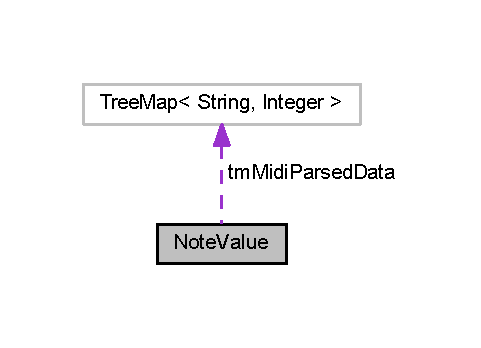
\includegraphics[width=231pt]{classcom_1_1lclion_1_1midiparser_1_1_note_value__coll__graph}
\end{center}
\end{figure}
\subsection*{Public Member Functions}
\begin{DoxyCompactItemize}
\item 
void \hyperlink{classcom_1_1lclion_1_1midiparser_1_1_note_value_a383ad3e4385be31e865bfe19f7d91050}{setup\+Notes\+By\+Quarter\+Note} (int \hyperlink{classcom_1_1lclion_1_1midiparser_1_1_note_value_ae639274224563b363fe8dc556cbbce62}{quarter\+Note})
\item 
String \hyperlink{classcom_1_1lclion_1_1midiparser_1_1_note_value_a92a1ecb736d0ecda2eea27d9181afac4}{determine\+Note\+Value} (long note\+Value)
\end{DoxyCompactItemize}
\subsection*{Protected Member Functions}
\begin{DoxyCompactItemize}
\item 
long \hyperlink{classcom_1_1lclion_1_1midiparser_1_1_note_value_a890f6abc3a9b2a24c4c0e2ce7d5ac790}{get\+Octuple\+Note} ()
\item 
long \hyperlink{classcom_1_1lclion_1_1midiparser_1_1_note_value_ad23ebd281c4fdf32ea9e528483cea923}{get\+Quadruple\+Note} ()
\item 
long \hyperlink{classcom_1_1lclion_1_1midiparser_1_1_note_value_a88753f5e9c5325cd14524672da0d81aa}{get\+Whole\+Note} ()
\item 
long \hyperlink{classcom_1_1lclion_1_1midiparser_1_1_note_value_af8a4a16e82f3799ace366de1756b6b4a}{get\+Half\+Note} ()
\item 
long \hyperlink{classcom_1_1lclion_1_1midiparser_1_1_note_value_a708af9e95f314d27580155ea8959fe45}{get\+Quarter\+Note} ()
\item 
long \hyperlink{classcom_1_1lclion_1_1midiparser_1_1_note_value_a66acedb007f8ce82a482502be7e2e506}{get\+Eighth\+Note} ()
\item 
long \hyperlink{classcom_1_1lclion_1_1midiparser_1_1_note_value_a280a5f4f04adf62c76efae5724afbd44}{get\+Sixteenth\+Note} ()
\item 
long \hyperlink{classcom_1_1lclion_1_1midiparser_1_1_note_value_aff4d51de807b98c18b7f44a00b0d531f}{get\+Thirty\+Second\+Note} ()
\item 
long \hyperlink{classcom_1_1lclion_1_1midiparser_1_1_note_value_a312d45f20b90755da158640695dab4fb}{get\+Sixty\+Fourth\+Note} ()
\item 
long \hyperlink{classcom_1_1lclion_1_1midiparser_1_1_note_value_ae3e0e3b611ea661f08502b3b6d645f76}{get\+Hundred\+Twenty\+Eighth\+Note} ()
\item 
long \hyperlink{classcom_1_1lclion_1_1midiparser_1_1_note_value_a3cac3598f0e435e9df344abc33005074}{get\+Two\+Hundred\+Fifty\+Sixth\+Note} ()
\end{DoxyCompactItemize}
\subsection*{Protected Attributes}
\begin{DoxyCompactItemize}
\item 
long \hyperlink{classcom_1_1lclion_1_1midiparser_1_1_note_value_a0fe4156c4e159f9a31683a59b06c1213}{octuple\+Note}
\item 
long \hyperlink{classcom_1_1lclion_1_1midiparser_1_1_note_value_ac77da61f39c85c427dda26cedd8d4f33}{quadruple\+Note}
\item 
long \hyperlink{classcom_1_1lclion_1_1midiparser_1_1_note_value_a2c13de9bc725e5050477c6b6dd2c2685}{whole\+Note}
\item 
long \hyperlink{classcom_1_1lclion_1_1midiparser_1_1_note_value_a9ec6410d8fdb73fe7b7f8ac085143899}{half\+Note}
\item 
long \hyperlink{classcom_1_1lclion_1_1midiparser_1_1_note_value_ae639274224563b363fe8dc556cbbce62}{quarter\+Note}
\item 
long \hyperlink{classcom_1_1lclion_1_1midiparser_1_1_note_value_a9e3dcd56ee8c1ab5bdcaa8fbb9288ba0}{eighth\+Note}
\item 
long \hyperlink{classcom_1_1lclion_1_1midiparser_1_1_note_value_af0442d9703406792637f35a3c4e2b130}{sixteenth\+Note}
\item 
long \hyperlink{classcom_1_1lclion_1_1midiparser_1_1_note_value_a2a933c01f9e22c17ce9a40d63a33f946}{thirty\+Second\+Note}
\item 
long \hyperlink{classcom_1_1lclion_1_1midiparser_1_1_note_value_aff6ebf47b5381550caaffc00fa985919}{sixty\+Fourth\+Note}
\item 
long \hyperlink{classcom_1_1lclion_1_1midiparser_1_1_note_value_a317ae100aa1c03b9c81ba01bd2f21e10}{hundred\+Twenty\+Eighth\+Note}
\item 
long \hyperlink{classcom_1_1lclion_1_1midiparser_1_1_note_value_a4a95369850429cf5d1cc019b0a88ae04}{two\+Hundred\+Fifty\+Sixth\+Note}
\end{DoxyCompactItemize}
\subsection*{Private Attributes}
\begin{DoxyCompactItemize}
\item 
Tree\+Map$<$ String, Integer $>$ \hyperlink{classcom_1_1lclion_1_1midiparser_1_1_note_value_a2c45af85892bf1a0526df4c6d66a27b7}{tm\+Midi\+Parsed\+Data} = null
\end{DoxyCompactItemize}


\subsection{Detailed Description}
Setups all notes and how long the notes last. 

\begin{DoxyAuthor}{Author}
L\+C Lion 
\end{DoxyAuthor}


\subsection{Member Function Documentation}
\hypertarget{classcom_1_1lclion_1_1midiparser_1_1_note_value_a92a1ecb736d0ecda2eea27d9181afac4}{\index{com\+::lclion\+::midiparser\+::\+Note\+Value@{com\+::lclion\+::midiparser\+::\+Note\+Value}!determine\+Note\+Value@{determine\+Note\+Value}}
\index{determine\+Note\+Value@{determine\+Note\+Value}!com\+::lclion\+::midiparser\+::\+Note\+Value@{com\+::lclion\+::midiparser\+::\+Note\+Value}}
\subsubsection[{determine\+Note\+Value}]{\setlength{\rightskip}{0pt plus 5cm}String determine\+Note\+Value (
\begin{DoxyParamCaption}
\item[{long}]{note\+Value}
\end{DoxyParamCaption}
)}}\label{classcom_1_1lclion_1_1midiparser_1_1_note_value_a92a1ecb736d0ecda2eea27d9181afac4}
\hypertarget{classcom_1_1lclion_1_1midiparser_1_1_note_value_a66acedb007f8ce82a482502be7e2e506}{\index{com\+::lclion\+::midiparser\+::\+Note\+Value@{com\+::lclion\+::midiparser\+::\+Note\+Value}!get\+Eighth\+Note@{get\+Eighth\+Note}}
\index{get\+Eighth\+Note@{get\+Eighth\+Note}!com\+::lclion\+::midiparser\+::\+Note\+Value@{com\+::lclion\+::midiparser\+::\+Note\+Value}}
\subsubsection[{get\+Eighth\+Note}]{\setlength{\rightskip}{0pt plus 5cm}long get\+Eighth\+Note (
\begin{DoxyParamCaption}
{}
\end{DoxyParamCaption}
)\hspace{0.3cm}{\ttfamily [protected]}}}\label{classcom_1_1lclion_1_1midiparser_1_1_note_value_a66acedb007f8ce82a482502be7e2e506}
\hypertarget{classcom_1_1lclion_1_1midiparser_1_1_note_value_af8a4a16e82f3799ace366de1756b6b4a}{\index{com\+::lclion\+::midiparser\+::\+Note\+Value@{com\+::lclion\+::midiparser\+::\+Note\+Value}!get\+Half\+Note@{get\+Half\+Note}}
\index{get\+Half\+Note@{get\+Half\+Note}!com\+::lclion\+::midiparser\+::\+Note\+Value@{com\+::lclion\+::midiparser\+::\+Note\+Value}}
\subsubsection[{get\+Half\+Note}]{\setlength{\rightskip}{0pt plus 5cm}long get\+Half\+Note (
\begin{DoxyParamCaption}
{}
\end{DoxyParamCaption}
)\hspace{0.3cm}{\ttfamily [protected]}}}\label{classcom_1_1lclion_1_1midiparser_1_1_note_value_af8a4a16e82f3799ace366de1756b6b4a}
\hypertarget{classcom_1_1lclion_1_1midiparser_1_1_note_value_ae3e0e3b611ea661f08502b3b6d645f76}{\index{com\+::lclion\+::midiparser\+::\+Note\+Value@{com\+::lclion\+::midiparser\+::\+Note\+Value}!get\+Hundred\+Twenty\+Eighth\+Note@{get\+Hundred\+Twenty\+Eighth\+Note}}
\index{get\+Hundred\+Twenty\+Eighth\+Note@{get\+Hundred\+Twenty\+Eighth\+Note}!com\+::lclion\+::midiparser\+::\+Note\+Value@{com\+::lclion\+::midiparser\+::\+Note\+Value}}
\subsubsection[{get\+Hundred\+Twenty\+Eighth\+Note}]{\setlength{\rightskip}{0pt plus 5cm}long get\+Hundred\+Twenty\+Eighth\+Note (
\begin{DoxyParamCaption}
{}
\end{DoxyParamCaption}
)\hspace{0.3cm}{\ttfamily [protected]}}}\label{classcom_1_1lclion_1_1midiparser_1_1_note_value_ae3e0e3b611ea661f08502b3b6d645f76}
\hypertarget{classcom_1_1lclion_1_1midiparser_1_1_note_value_a890f6abc3a9b2a24c4c0e2ce7d5ac790}{\index{com\+::lclion\+::midiparser\+::\+Note\+Value@{com\+::lclion\+::midiparser\+::\+Note\+Value}!get\+Octuple\+Note@{get\+Octuple\+Note}}
\index{get\+Octuple\+Note@{get\+Octuple\+Note}!com\+::lclion\+::midiparser\+::\+Note\+Value@{com\+::lclion\+::midiparser\+::\+Note\+Value}}
\subsubsection[{get\+Octuple\+Note}]{\setlength{\rightskip}{0pt plus 5cm}long get\+Octuple\+Note (
\begin{DoxyParamCaption}
{}
\end{DoxyParamCaption}
)\hspace{0.3cm}{\ttfamily [protected]}}}\label{classcom_1_1lclion_1_1midiparser_1_1_note_value_a890f6abc3a9b2a24c4c0e2ce7d5ac790}
\hypertarget{classcom_1_1lclion_1_1midiparser_1_1_note_value_ad23ebd281c4fdf32ea9e528483cea923}{\index{com\+::lclion\+::midiparser\+::\+Note\+Value@{com\+::lclion\+::midiparser\+::\+Note\+Value}!get\+Quadruple\+Note@{get\+Quadruple\+Note}}
\index{get\+Quadruple\+Note@{get\+Quadruple\+Note}!com\+::lclion\+::midiparser\+::\+Note\+Value@{com\+::lclion\+::midiparser\+::\+Note\+Value}}
\subsubsection[{get\+Quadruple\+Note}]{\setlength{\rightskip}{0pt plus 5cm}long get\+Quadruple\+Note (
\begin{DoxyParamCaption}
{}
\end{DoxyParamCaption}
)\hspace{0.3cm}{\ttfamily [protected]}}}\label{classcom_1_1lclion_1_1midiparser_1_1_note_value_ad23ebd281c4fdf32ea9e528483cea923}
\hypertarget{classcom_1_1lclion_1_1midiparser_1_1_note_value_a708af9e95f314d27580155ea8959fe45}{\index{com\+::lclion\+::midiparser\+::\+Note\+Value@{com\+::lclion\+::midiparser\+::\+Note\+Value}!get\+Quarter\+Note@{get\+Quarter\+Note}}
\index{get\+Quarter\+Note@{get\+Quarter\+Note}!com\+::lclion\+::midiparser\+::\+Note\+Value@{com\+::lclion\+::midiparser\+::\+Note\+Value}}
\subsubsection[{get\+Quarter\+Note}]{\setlength{\rightskip}{0pt plus 5cm}long get\+Quarter\+Note (
\begin{DoxyParamCaption}
{}
\end{DoxyParamCaption}
)\hspace{0.3cm}{\ttfamily [protected]}}}\label{classcom_1_1lclion_1_1midiparser_1_1_note_value_a708af9e95f314d27580155ea8959fe45}
\hypertarget{classcom_1_1lclion_1_1midiparser_1_1_note_value_a280a5f4f04adf62c76efae5724afbd44}{\index{com\+::lclion\+::midiparser\+::\+Note\+Value@{com\+::lclion\+::midiparser\+::\+Note\+Value}!get\+Sixteenth\+Note@{get\+Sixteenth\+Note}}
\index{get\+Sixteenth\+Note@{get\+Sixteenth\+Note}!com\+::lclion\+::midiparser\+::\+Note\+Value@{com\+::lclion\+::midiparser\+::\+Note\+Value}}
\subsubsection[{get\+Sixteenth\+Note}]{\setlength{\rightskip}{0pt plus 5cm}long get\+Sixteenth\+Note (
\begin{DoxyParamCaption}
{}
\end{DoxyParamCaption}
)\hspace{0.3cm}{\ttfamily [protected]}}}\label{classcom_1_1lclion_1_1midiparser_1_1_note_value_a280a5f4f04adf62c76efae5724afbd44}
\hypertarget{classcom_1_1lclion_1_1midiparser_1_1_note_value_a312d45f20b90755da158640695dab4fb}{\index{com\+::lclion\+::midiparser\+::\+Note\+Value@{com\+::lclion\+::midiparser\+::\+Note\+Value}!get\+Sixty\+Fourth\+Note@{get\+Sixty\+Fourth\+Note}}
\index{get\+Sixty\+Fourth\+Note@{get\+Sixty\+Fourth\+Note}!com\+::lclion\+::midiparser\+::\+Note\+Value@{com\+::lclion\+::midiparser\+::\+Note\+Value}}
\subsubsection[{get\+Sixty\+Fourth\+Note}]{\setlength{\rightskip}{0pt plus 5cm}long get\+Sixty\+Fourth\+Note (
\begin{DoxyParamCaption}
{}
\end{DoxyParamCaption}
)\hspace{0.3cm}{\ttfamily [protected]}}}\label{classcom_1_1lclion_1_1midiparser_1_1_note_value_a312d45f20b90755da158640695dab4fb}
\hypertarget{classcom_1_1lclion_1_1midiparser_1_1_note_value_aff4d51de807b98c18b7f44a00b0d531f}{\index{com\+::lclion\+::midiparser\+::\+Note\+Value@{com\+::lclion\+::midiparser\+::\+Note\+Value}!get\+Thirty\+Second\+Note@{get\+Thirty\+Second\+Note}}
\index{get\+Thirty\+Second\+Note@{get\+Thirty\+Second\+Note}!com\+::lclion\+::midiparser\+::\+Note\+Value@{com\+::lclion\+::midiparser\+::\+Note\+Value}}
\subsubsection[{get\+Thirty\+Second\+Note}]{\setlength{\rightskip}{0pt plus 5cm}long get\+Thirty\+Second\+Note (
\begin{DoxyParamCaption}
{}
\end{DoxyParamCaption}
)\hspace{0.3cm}{\ttfamily [protected]}}}\label{classcom_1_1lclion_1_1midiparser_1_1_note_value_aff4d51de807b98c18b7f44a00b0d531f}
\hypertarget{classcom_1_1lclion_1_1midiparser_1_1_note_value_a3cac3598f0e435e9df344abc33005074}{\index{com\+::lclion\+::midiparser\+::\+Note\+Value@{com\+::lclion\+::midiparser\+::\+Note\+Value}!get\+Two\+Hundred\+Fifty\+Sixth\+Note@{get\+Two\+Hundred\+Fifty\+Sixth\+Note}}
\index{get\+Two\+Hundred\+Fifty\+Sixth\+Note@{get\+Two\+Hundred\+Fifty\+Sixth\+Note}!com\+::lclion\+::midiparser\+::\+Note\+Value@{com\+::lclion\+::midiparser\+::\+Note\+Value}}
\subsubsection[{get\+Two\+Hundred\+Fifty\+Sixth\+Note}]{\setlength{\rightskip}{0pt plus 5cm}long get\+Two\+Hundred\+Fifty\+Sixth\+Note (
\begin{DoxyParamCaption}
{}
\end{DoxyParamCaption}
)\hspace{0.3cm}{\ttfamily [protected]}}}\label{classcom_1_1lclion_1_1midiparser_1_1_note_value_a3cac3598f0e435e9df344abc33005074}
\hypertarget{classcom_1_1lclion_1_1midiparser_1_1_note_value_a88753f5e9c5325cd14524672da0d81aa}{\index{com\+::lclion\+::midiparser\+::\+Note\+Value@{com\+::lclion\+::midiparser\+::\+Note\+Value}!get\+Whole\+Note@{get\+Whole\+Note}}
\index{get\+Whole\+Note@{get\+Whole\+Note}!com\+::lclion\+::midiparser\+::\+Note\+Value@{com\+::lclion\+::midiparser\+::\+Note\+Value}}
\subsubsection[{get\+Whole\+Note}]{\setlength{\rightskip}{0pt plus 5cm}long get\+Whole\+Note (
\begin{DoxyParamCaption}
{}
\end{DoxyParamCaption}
)\hspace{0.3cm}{\ttfamily [protected]}}}\label{classcom_1_1lclion_1_1midiparser_1_1_note_value_a88753f5e9c5325cd14524672da0d81aa}
\hypertarget{classcom_1_1lclion_1_1midiparser_1_1_note_value_a383ad3e4385be31e865bfe19f7d91050}{\index{com\+::lclion\+::midiparser\+::\+Note\+Value@{com\+::lclion\+::midiparser\+::\+Note\+Value}!setup\+Notes\+By\+Quarter\+Note@{setup\+Notes\+By\+Quarter\+Note}}
\index{setup\+Notes\+By\+Quarter\+Note@{setup\+Notes\+By\+Quarter\+Note}!com\+::lclion\+::midiparser\+::\+Note\+Value@{com\+::lclion\+::midiparser\+::\+Note\+Value}}
\subsubsection[{setup\+Notes\+By\+Quarter\+Note}]{\setlength{\rightskip}{0pt plus 5cm}void setup\+Notes\+By\+Quarter\+Note (
\begin{DoxyParamCaption}
\item[{int}]{quarter\+Note}
\end{DoxyParamCaption}
)}}\label{classcom_1_1lclion_1_1midiparser_1_1_note_value_a383ad3e4385be31e865bfe19f7d91050}


\subsection{Member Data Documentation}
\hypertarget{classcom_1_1lclion_1_1midiparser_1_1_note_value_a9e3dcd56ee8c1ab5bdcaa8fbb9288ba0}{\index{com\+::lclion\+::midiparser\+::\+Note\+Value@{com\+::lclion\+::midiparser\+::\+Note\+Value}!eighth\+Note@{eighth\+Note}}
\index{eighth\+Note@{eighth\+Note}!com\+::lclion\+::midiparser\+::\+Note\+Value@{com\+::lclion\+::midiparser\+::\+Note\+Value}}
\subsubsection[{eighth\+Note}]{\setlength{\rightskip}{0pt plus 5cm}long eighth\+Note\hspace{0.3cm}{\ttfamily [protected]}}}\label{classcom_1_1lclion_1_1midiparser_1_1_note_value_a9e3dcd56ee8c1ab5bdcaa8fbb9288ba0}
\hypertarget{classcom_1_1lclion_1_1midiparser_1_1_note_value_a9ec6410d8fdb73fe7b7f8ac085143899}{\index{com\+::lclion\+::midiparser\+::\+Note\+Value@{com\+::lclion\+::midiparser\+::\+Note\+Value}!half\+Note@{half\+Note}}
\index{half\+Note@{half\+Note}!com\+::lclion\+::midiparser\+::\+Note\+Value@{com\+::lclion\+::midiparser\+::\+Note\+Value}}
\subsubsection[{half\+Note}]{\setlength{\rightskip}{0pt plus 5cm}long half\+Note\hspace{0.3cm}{\ttfamily [protected]}}}\label{classcom_1_1lclion_1_1midiparser_1_1_note_value_a9ec6410d8fdb73fe7b7f8ac085143899}
\hypertarget{classcom_1_1lclion_1_1midiparser_1_1_note_value_a317ae100aa1c03b9c81ba01bd2f21e10}{\index{com\+::lclion\+::midiparser\+::\+Note\+Value@{com\+::lclion\+::midiparser\+::\+Note\+Value}!hundred\+Twenty\+Eighth\+Note@{hundred\+Twenty\+Eighth\+Note}}
\index{hundred\+Twenty\+Eighth\+Note@{hundred\+Twenty\+Eighth\+Note}!com\+::lclion\+::midiparser\+::\+Note\+Value@{com\+::lclion\+::midiparser\+::\+Note\+Value}}
\subsubsection[{hundred\+Twenty\+Eighth\+Note}]{\setlength{\rightskip}{0pt plus 5cm}long hundred\+Twenty\+Eighth\+Note\hspace{0.3cm}{\ttfamily [protected]}}}\label{classcom_1_1lclion_1_1midiparser_1_1_note_value_a317ae100aa1c03b9c81ba01bd2f21e10}
\hypertarget{classcom_1_1lclion_1_1midiparser_1_1_note_value_a0fe4156c4e159f9a31683a59b06c1213}{\index{com\+::lclion\+::midiparser\+::\+Note\+Value@{com\+::lclion\+::midiparser\+::\+Note\+Value}!octuple\+Note@{octuple\+Note}}
\index{octuple\+Note@{octuple\+Note}!com\+::lclion\+::midiparser\+::\+Note\+Value@{com\+::lclion\+::midiparser\+::\+Note\+Value}}
\subsubsection[{octuple\+Note}]{\setlength{\rightskip}{0pt plus 5cm}long octuple\+Note\hspace{0.3cm}{\ttfamily [protected]}}}\label{classcom_1_1lclion_1_1midiparser_1_1_note_value_a0fe4156c4e159f9a31683a59b06c1213}
\hypertarget{classcom_1_1lclion_1_1midiparser_1_1_note_value_ac77da61f39c85c427dda26cedd8d4f33}{\index{com\+::lclion\+::midiparser\+::\+Note\+Value@{com\+::lclion\+::midiparser\+::\+Note\+Value}!quadruple\+Note@{quadruple\+Note}}
\index{quadruple\+Note@{quadruple\+Note}!com\+::lclion\+::midiparser\+::\+Note\+Value@{com\+::lclion\+::midiparser\+::\+Note\+Value}}
\subsubsection[{quadruple\+Note}]{\setlength{\rightskip}{0pt plus 5cm}long quadruple\+Note\hspace{0.3cm}{\ttfamily [protected]}}}\label{classcom_1_1lclion_1_1midiparser_1_1_note_value_ac77da61f39c85c427dda26cedd8d4f33}
\hypertarget{classcom_1_1lclion_1_1midiparser_1_1_note_value_ae639274224563b363fe8dc556cbbce62}{\index{com\+::lclion\+::midiparser\+::\+Note\+Value@{com\+::lclion\+::midiparser\+::\+Note\+Value}!quarter\+Note@{quarter\+Note}}
\index{quarter\+Note@{quarter\+Note}!com\+::lclion\+::midiparser\+::\+Note\+Value@{com\+::lclion\+::midiparser\+::\+Note\+Value}}
\subsubsection[{quarter\+Note}]{\setlength{\rightskip}{0pt plus 5cm}long quarter\+Note\hspace{0.3cm}{\ttfamily [protected]}}}\label{classcom_1_1lclion_1_1midiparser_1_1_note_value_ae639274224563b363fe8dc556cbbce62}
\hypertarget{classcom_1_1lclion_1_1midiparser_1_1_note_value_af0442d9703406792637f35a3c4e2b130}{\index{com\+::lclion\+::midiparser\+::\+Note\+Value@{com\+::lclion\+::midiparser\+::\+Note\+Value}!sixteenth\+Note@{sixteenth\+Note}}
\index{sixteenth\+Note@{sixteenth\+Note}!com\+::lclion\+::midiparser\+::\+Note\+Value@{com\+::lclion\+::midiparser\+::\+Note\+Value}}
\subsubsection[{sixteenth\+Note}]{\setlength{\rightskip}{0pt plus 5cm}long sixteenth\+Note\hspace{0.3cm}{\ttfamily [protected]}}}\label{classcom_1_1lclion_1_1midiparser_1_1_note_value_af0442d9703406792637f35a3c4e2b130}
\hypertarget{classcom_1_1lclion_1_1midiparser_1_1_note_value_aff6ebf47b5381550caaffc00fa985919}{\index{com\+::lclion\+::midiparser\+::\+Note\+Value@{com\+::lclion\+::midiparser\+::\+Note\+Value}!sixty\+Fourth\+Note@{sixty\+Fourth\+Note}}
\index{sixty\+Fourth\+Note@{sixty\+Fourth\+Note}!com\+::lclion\+::midiparser\+::\+Note\+Value@{com\+::lclion\+::midiparser\+::\+Note\+Value}}
\subsubsection[{sixty\+Fourth\+Note}]{\setlength{\rightskip}{0pt plus 5cm}long sixty\+Fourth\+Note\hspace{0.3cm}{\ttfamily [protected]}}}\label{classcom_1_1lclion_1_1midiparser_1_1_note_value_aff6ebf47b5381550caaffc00fa985919}
\hypertarget{classcom_1_1lclion_1_1midiparser_1_1_note_value_a2a933c01f9e22c17ce9a40d63a33f946}{\index{com\+::lclion\+::midiparser\+::\+Note\+Value@{com\+::lclion\+::midiparser\+::\+Note\+Value}!thirty\+Second\+Note@{thirty\+Second\+Note}}
\index{thirty\+Second\+Note@{thirty\+Second\+Note}!com\+::lclion\+::midiparser\+::\+Note\+Value@{com\+::lclion\+::midiparser\+::\+Note\+Value}}
\subsubsection[{thirty\+Second\+Note}]{\setlength{\rightskip}{0pt plus 5cm}long thirty\+Second\+Note\hspace{0.3cm}{\ttfamily [protected]}}}\label{classcom_1_1lclion_1_1midiparser_1_1_note_value_a2a933c01f9e22c17ce9a40d63a33f946}
\hypertarget{classcom_1_1lclion_1_1midiparser_1_1_note_value_a2c45af85892bf1a0526df4c6d66a27b7}{\index{com\+::lclion\+::midiparser\+::\+Note\+Value@{com\+::lclion\+::midiparser\+::\+Note\+Value}!tm\+Midi\+Parsed\+Data@{tm\+Midi\+Parsed\+Data}}
\index{tm\+Midi\+Parsed\+Data@{tm\+Midi\+Parsed\+Data}!com\+::lclion\+::midiparser\+::\+Note\+Value@{com\+::lclion\+::midiparser\+::\+Note\+Value}}
\subsubsection[{tm\+Midi\+Parsed\+Data}]{\setlength{\rightskip}{0pt plus 5cm}Tree\+Map$<$String, Integer$>$ tm\+Midi\+Parsed\+Data = null\hspace{0.3cm}{\ttfamily [private]}}}\label{classcom_1_1lclion_1_1midiparser_1_1_note_value_a2c45af85892bf1a0526df4c6d66a27b7}
\hypertarget{classcom_1_1lclion_1_1midiparser_1_1_note_value_a4a95369850429cf5d1cc019b0a88ae04}{\index{com\+::lclion\+::midiparser\+::\+Note\+Value@{com\+::lclion\+::midiparser\+::\+Note\+Value}!two\+Hundred\+Fifty\+Sixth\+Note@{two\+Hundred\+Fifty\+Sixth\+Note}}
\index{two\+Hundred\+Fifty\+Sixth\+Note@{two\+Hundred\+Fifty\+Sixth\+Note}!com\+::lclion\+::midiparser\+::\+Note\+Value@{com\+::lclion\+::midiparser\+::\+Note\+Value}}
\subsubsection[{two\+Hundred\+Fifty\+Sixth\+Note}]{\setlength{\rightskip}{0pt plus 5cm}long two\+Hundred\+Fifty\+Sixth\+Note\hspace{0.3cm}{\ttfamily [protected]}}}\label{classcom_1_1lclion_1_1midiparser_1_1_note_value_a4a95369850429cf5d1cc019b0a88ae04}
\hypertarget{classcom_1_1lclion_1_1midiparser_1_1_note_value_a2c13de9bc725e5050477c6b6dd2c2685}{\index{com\+::lclion\+::midiparser\+::\+Note\+Value@{com\+::lclion\+::midiparser\+::\+Note\+Value}!whole\+Note@{whole\+Note}}
\index{whole\+Note@{whole\+Note}!com\+::lclion\+::midiparser\+::\+Note\+Value@{com\+::lclion\+::midiparser\+::\+Note\+Value}}
\subsubsection[{whole\+Note}]{\setlength{\rightskip}{0pt plus 5cm}long whole\+Note\hspace{0.3cm}{\ttfamily [protected]}}}\label{classcom_1_1lclion_1_1midiparser_1_1_note_value_a2c13de9bc725e5050477c6b6dd2c2685}


The documentation for this class was generated from the following file\+:\begin{DoxyCompactItemize}
\item 
src/com/lclion/midiparser/\hyperlink{_note_value_8java}{Note\+Value.\+java}\end{DoxyCompactItemize}

\hypertarget{classcom_1_1lclion_1_1midiparser_1_1_patch_converter}{\section{Patch\+Converter Class Reference}
\label{classcom_1_1lclion_1_1midiparser_1_1_patch_converter}\index{Patch\+Converter@{Patch\+Converter}}
}


Convert M\+I\+D\+I Patch Numbers to corresponding instrument name.  




Collaboration diagram for Patch\+Converter\+:\nopagebreak
\begin{figure}[H]
\begin{center}
\leavevmode
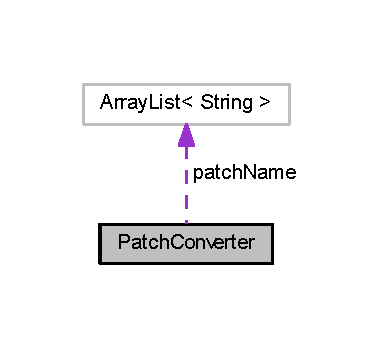
\includegraphics[width=183pt]{classcom_1_1lclion_1_1midiparser_1_1_patch_converter__coll__graph}
\end{center}
\end{figure}
\subsection*{Public Member Functions}
\begin{DoxyCompactItemize}
\item 
\hyperlink{classcom_1_1lclion_1_1midiparser_1_1_patch_converter_a3fa7bf625d76c88c6703326ceb1402e5}{Patch\+Converter} ()
\item 
String \hyperlink{classcom_1_1lclion_1_1midiparser_1_1_patch_converter_a6b0d3c53592bd1ab882a7ff96c1f368e}{get\+Patch\+Name} (int patch\+Num)
\end{DoxyCompactItemize}
\subsection*{Static Private Attributes}
\begin{DoxyCompactItemize}
\item 
static Array\+List$<$ String $>$ \hyperlink{classcom_1_1lclion_1_1midiparser_1_1_patch_converter_a62653567f7df39fd70881a4e4c6b6047}{patch\+Name} = new Array\+List$<$String$>$()
\end{DoxyCompactItemize}


\subsection{Detailed Description}
Convert M\+I\+D\+I Patch Numbers to corresponding instrument name. 

\begin{DoxyAuthor}{Author}
L\+C Lion 
\end{DoxyAuthor}


\subsection{Constructor \& Destructor Documentation}
\hypertarget{classcom_1_1lclion_1_1midiparser_1_1_patch_converter_a3fa7bf625d76c88c6703326ceb1402e5}{\index{com\+::lclion\+::midiparser\+::\+Patch\+Converter@{com\+::lclion\+::midiparser\+::\+Patch\+Converter}!Patch\+Converter@{Patch\+Converter}}
\index{Patch\+Converter@{Patch\+Converter}!com\+::lclion\+::midiparser\+::\+Patch\+Converter@{com\+::lclion\+::midiparser\+::\+Patch\+Converter}}
\subsubsection[{Patch\+Converter}]{\setlength{\rightskip}{0pt plus 5cm}{\bf Patch\+Converter} (
\begin{DoxyParamCaption}
{}
\end{DoxyParamCaption}
)}}\label{classcom_1_1lclion_1_1midiparser_1_1_patch_converter_a3fa7bf625d76c88c6703326ceb1402e5}


\subsection{Member Function Documentation}
\hypertarget{classcom_1_1lclion_1_1midiparser_1_1_patch_converter_a6b0d3c53592bd1ab882a7ff96c1f368e}{\index{com\+::lclion\+::midiparser\+::\+Patch\+Converter@{com\+::lclion\+::midiparser\+::\+Patch\+Converter}!get\+Patch\+Name@{get\+Patch\+Name}}
\index{get\+Patch\+Name@{get\+Patch\+Name}!com\+::lclion\+::midiparser\+::\+Patch\+Converter@{com\+::lclion\+::midiparser\+::\+Patch\+Converter}}
\subsubsection[{get\+Patch\+Name}]{\setlength{\rightskip}{0pt plus 5cm}String get\+Patch\+Name (
\begin{DoxyParamCaption}
\item[{int}]{patch\+Num}
\end{DoxyParamCaption}
)}}\label{classcom_1_1lclion_1_1midiparser_1_1_patch_converter_a6b0d3c53592bd1ab882a7ff96c1f368e}


\subsection{Member Data Documentation}
\hypertarget{classcom_1_1lclion_1_1midiparser_1_1_patch_converter_a62653567f7df39fd70881a4e4c6b6047}{\index{com\+::lclion\+::midiparser\+::\+Patch\+Converter@{com\+::lclion\+::midiparser\+::\+Patch\+Converter}!patch\+Name@{patch\+Name}}
\index{patch\+Name@{patch\+Name}!com\+::lclion\+::midiparser\+::\+Patch\+Converter@{com\+::lclion\+::midiparser\+::\+Patch\+Converter}}
\subsubsection[{patch\+Name}]{\setlength{\rightskip}{0pt plus 5cm}Array\+List$<$String$>$ patch\+Name = new Array\+List$<$String$>$()\hspace{0.3cm}{\ttfamily [static]}, {\ttfamily [private]}}}\label{classcom_1_1lclion_1_1midiparser_1_1_patch_converter_a62653567f7df39fd70881a4e4c6b6047}


The documentation for this class was generated from the following file\+:\begin{DoxyCompactItemize}
\item 
src/com/lclion/midiparser/\hyperlink{_patch_converter_8java}{Patch\+Converter.\+java}\end{DoxyCompactItemize}

\hypertarget{classcom_1_1lclion_1_1midiparser_1_1_string_notes_parser}{\section{String\+Notes\+Parser Class Reference}
\label{classcom_1_1lclion_1_1midiparser_1_1_string_notes_parser}\index{String\+Notes\+Parser@{String\+Notes\+Parser}}
}


Collaboration diagram for String\+Notes\+Parser\+:\nopagebreak
\begin{figure}[H]
\begin{center}
\leavevmode
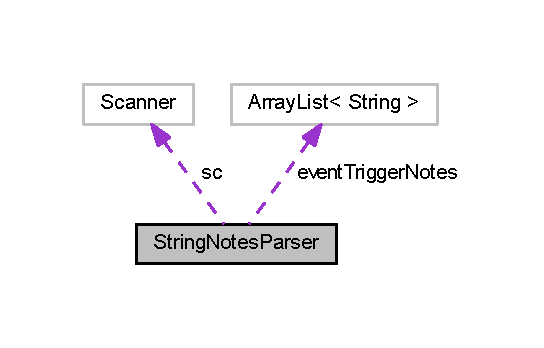
\includegraphics[width=261pt]{classcom_1_1lclion_1_1midiparser_1_1_string_notes_parser__coll__graph}
\end{center}
\end{figure}
\subsection*{Public Member Functions}
\begin{DoxyCompactItemize}
\item 
\hyperlink{classcom_1_1lclion_1_1midiparser_1_1_string_notes_parser_a598cb026a05b3ea58cc9d5b9124c0001}{String\+Notes\+Parser} (String \hyperlink{classcom_1_1lclion_1_1midiparser_1_1_string_notes_parser_affda1ac66ff7fe4869f395974d539adc}{string\+To\+Parse})
\item 
String \hyperlink{classcom_1_1lclion_1_1midiparser_1_1_string_notes_parser_a01b964ea248967218b88e1d6558592cd}{get\+Next\+Notes} ()
\item 
int \hyperlink{classcom_1_1lclion_1_1midiparser_1_1_string_notes_parser_a16e67d67362fc128a3bd84faccda8422}{get\+Off\+Set} ()
\item 
int \hyperlink{classcom_1_1lclion_1_1midiparser_1_1_string_notes_parser_aab0d4bbd0884d04dbe281cc2b9d21206}{get\+Length} ()
\end{DoxyCompactItemize}
\subsection*{Private Member Functions}
\begin{DoxyCompactItemize}
\item 
void \hyperlink{classcom_1_1lclion_1_1midiparser_1_1_string_notes_parser_a2c58052b399ad0a04348e645f46f527b}{setup\+Event\+Trigger\+Notes} ()
\end{DoxyCompactItemize}
\subsection*{Private Attributes}
\begin{DoxyCompactItemize}
\item 
String \hyperlink{classcom_1_1lclion_1_1midiparser_1_1_string_notes_parser_affda1ac66ff7fe4869f395974d539adc}{string\+To\+Parse} = null
\item 
Scanner \hyperlink{classcom_1_1lclion_1_1midiparser_1_1_string_notes_parser_a851d4b6928a1fc6d70a295c89e42f9d9}{sc} = null
\item 
Array\+List$<$ String $>$ \hyperlink{classcom_1_1lclion_1_1midiparser_1_1_string_notes_parser_a0cbdfa4f6c165959c00f71afb7a4b65e}{event\+Trigger\+Notes} = new Array\+List$<$String$>$()
\item 
int \hyperlink{classcom_1_1lclion_1_1midiparser_1_1_string_notes_parser_a617a47c70795bcff659815ad0efd2266}{counter} = 0
\end{DoxyCompactItemize}


\subsection{Constructor \& Destructor Documentation}
\hypertarget{classcom_1_1lclion_1_1midiparser_1_1_string_notes_parser_a598cb026a05b3ea58cc9d5b9124c0001}{\index{com\+::lclion\+::midiparser\+::\+String\+Notes\+Parser@{com\+::lclion\+::midiparser\+::\+String\+Notes\+Parser}!String\+Notes\+Parser@{String\+Notes\+Parser}}
\index{String\+Notes\+Parser@{String\+Notes\+Parser}!com\+::lclion\+::midiparser\+::\+String\+Notes\+Parser@{com\+::lclion\+::midiparser\+::\+String\+Notes\+Parser}}
\subsubsection[{String\+Notes\+Parser}]{\setlength{\rightskip}{0pt plus 5cm}{\bf String\+Notes\+Parser} (
\begin{DoxyParamCaption}
\item[{String}]{string\+To\+Parse}
\end{DoxyParamCaption}
)}}\label{classcom_1_1lclion_1_1midiparser_1_1_string_notes_parser_a598cb026a05b3ea58cc9d5b9124c0001}


Here is the call graph for this function\+:\nopagebreak
\begin{figure}[H]
\begin{center}
\leavevmode
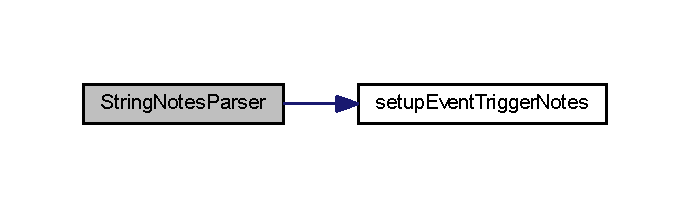
\includegraphics[width=331pt]{classcom_1_1lclion_1_1midiparser_1_1_string_notes_parser_a598cb026a05b3ea58cc9d5b9124c0001_cgraph}
\end{center}
\end{figure}




\subsection{Member Function Documentation}
\hypertarget{classcom_1_1lclion_1_1midiparser_1_1_string_notes_parser_aab0d4bbd0884d04dbe281cc2b9d21206}{\index{com\+::lclion\+::midiparser\+::\+String\+Notes\+Parser@{com\+::lclion\+::midiparser\+::\+String\+Notes\+Parser}!get\+Length@{get\+Length}}
\index{get\+Length@{get\+Length}!com\+::lclion\+::midiparser\+::\+String\+Notes\+Parser@{com\+::lclion\+::midiparser\+::\+String\+Notes\+Parser}}
\subsubsection[{get\+Length}]{\setlength{\rightskip}{0pt plus 5cm}int get\+Length (
\begin{DoxyParamCaption}
{}
\end{DoxyParamCaption}
)}}\label{classcom_1_1lclion_1_1midiparser_1_1_string_notes_parser_aab0d4bbd0884d04dbe281cc2b9d21206}
\hypertarget{classcom_1_1lclion_1_1midiparser_1_1_string_notes_parser_a01b964ea248967218b88e1d6558592cd}{\index{com\+::lclion\+::midiparser\+::\+String\+Notes\+Parser@{com\+::lclion\+::midiparser\+::\+String\+Notes\+Parser}!get\+Next\+Notes@{get\+Next\+Notes}}
\index{get\+Next\+Notes@{get\+Next\+Notes}!com\+::lclion\+::midiparser\+::\+String\+Notes\+Parser@{com\+::lclion\+::midiparser\+::\+String\+Notes\+Parser}}
\subsubsection[{get\+Next\+Notes}]{\setlength{\rightskip}{0pt plus 5cm}String get\+Next\+Notes (
\begin{DoxyParamCaption}
{}
\end{DoxyParamCaption}
)}}\label{classcom_1_1lclion_1_1midiparser_1_1_string_notes_parser_a01b964ea248967218b88e1d6558592cd}
\hypertarget{classcom_1_1lclion_1_1midiparser_1_1_string_notes_parser_a16e67d67362fc128a3bd84faccda8422}{\index{com\+::lclion\+::midiparser\+::\+String\+Notes\+Parser@{com\+::lclion\+::midiparser\+::\+String\+Notes\+Parser}!get\+Off\+Set@{get\+Off\+Set}}
\index{get\+Off\+Set@{get\+Off\+Set}!com\+::lclion\+::midiparser\+::\+String\+Notes\+Parser@{com\+::lclion\+::midiparser\+::\+String\+Notes\+Parser}}
\subsubsection[{get\+Off\+Set}]{\setlength{\rightskip}{0pt plus 5cm}int get\+Off\+Set (
\begin{DoxyParamCaption}
{}
\end{DoxyParamCaption}
)}}\label{classcom_1_1lclion_1_1midiparser_1_1_string_notes_parser_a16e67d67362fc128a3bd84faccda8422}
\hypertarget{classcom_1_1lclion_1_1midiparser_1_1_string_notes_parser_a2c58052b399ad0a04348e645f46f527b}{\index{com\+::lclion\+::midiparser\+::\+String\+Notes\+Parser@{com\+::lclion\+::midiparser\+::\+String\+Notes\+Parser}!setup\+Event\+Trigger\+Notes@{setup\+Event\+Trigger\+Notes}}
\index{setup\+Event\+Trigger\+Notes@{setup\+Event\+Trigger\+Notes}!com\+::lclion\+::midiparser\+::\+String\+Notes\+Parser@{com\+::lclion\+::midiparser\+::\+String\+Notes\+Parser}}
\subsubsection[{setup\+Event\+Trigger\+Notes}]{\setlength{\rightskip}{0pt plus 5cm}void setup\+Event\+Trigger\+Notes (
\begin{DoxyParamCaption}
{}
\end{DoxyParamCaption}
)\hspace{0.3cm}{\ttfamily [private]}}}\label{classcom_1_1lclion_1_1midiparser_1_1_string_notes_parser_a2c58052b399ad0a04348e645f46f527b}


\subsection{Member Data Documentation}
\hypertarget{classcom_1_1lclion_1_1midiparser_1_1_string_notes_parser_a617a47c70795bcff659815ad0efd2266}{\index{com\+::lclion\+::midiparser\+::\+String\+Notes\+Parser@{com\+::lclion\+::midiparser\+::\+String\+Notes\+Parser}!counter@{counter}}
\index{counter@{counter}!com\+::lclion\+::midiparser\+::\+String\+Notes\+Parser@{com\+::lclion\+::midiparser\+::\+String\+Notes\+Parser}}
\subsubsection[{counter}]{\setlength{\rightskip}{0pt plus 5cm}int counter = 0\hspace{0.3cm}{\ttfamily [private]}}}\label{classcom_1_1lclion_1_1midiparser_1_1_string_notes_parser_a617a47c70795bcff659815ad0efd2266}
\hypertarget{classcom_1_1lclion_1_1midiparser_1_1_string_notes_parser_a0cbdfa4f6c165959c00f71afb7a4b65e}{\index{com\+::lclion\+::midiparser\+::\+String\+Notes\+Parser@{com\+::lclion\+::midiparser\+::\+String\+Notes\+Parser}!event\+Trigger\+Notes@{event\+Trigger\+Notes}}
\index{event\+Trigger\+Notes@{event\+Trigger\+Notes}!com\+::lclion\+::midiparser\+::\+String\+Notes\+Parser@{com\+::lclion\+::midiparser\+::\+String\+Notes\+Parser}}
\subsubsection[{event\+Trigger\+Notes}]{\setlength{\rightskip}{0pt plus 5cm}Array\+List$<$String$>$ event\+Trigger\+Notes = new Array\+List$<$String$>$()\hspace{0.3cm}{\ttfamily [private]}}}\label{classcom_1_1lclion_1_1midiparser_1_1_string_notes_parser_a0cbdfa4f6c165959c00f71afb7a4b65e}
\hypertarget{classcom_1_1lclion_1_1midiparser_1_1_string_notes_parser_a851d4b6928a1fc6d70a295c89e42f9d9}{\index{com\+::lclion\+::midiparser\+::\+String\+Notes\+Parser@{com\+::lclion\+::midiparser\+::\+String\+Notes\+Parser}!sc@{sc}}
\index{sc@{sc}!com\+::lclion\+::midiparser\+::\+String\+Notes\+Parser@{com\+::lclion\+::midiparser\+::\+String\+Notes\+Parser}}
\subsubsection[{sc}]{\setlength{\rightskip}{0pt plus 5cm}Scanner sc = null\hspace{0.3cm}{\ttfamily [private]}}}\label{classcom_1_1lclion_1_1midiparser_1_1_string_notes_parser_a851d4b6928a1fc6d70a295c89e42f9d9}
\hypertarget{classcom_1_1lclion_1_1midiparser_1_1_string_notes_parser_affda1ac66ff7fe4869f395974d539adc}{\index{com\+::lclion\+::midiparser\+::\+String\+Notes\+Parser@{com\+::lclion\+::midiparser\+::\+String\+Notes\+Parser}!string\+To\+Parse@{string\+To\+Parse}}
\index{string\+To\+Parse@{string\+To\+Parse}!com\+::lclion\+::midiparser\+::\+String\+Notes\+Parser@{com\+::lclion\+::midiparser\+::\+String\+Notes\+Parser}}
\subsubsection[{string\+To\+Parse}]{\setlength{\rightskip}{0pt plus 5cm}String string\+To\+Parse = null\hspace{0.3cm}{\ttfamily [private]}}}\label{classcom_1_1lclion_1_1midiparser_1_1_string_notes_parser_affda1ac66ff7fe4869f395974d539adc}


The documentation for this class was generated from the following file\+:\begin{DoxyCompactItemize}
\item 
src/com/lclion/midiparser/\hyperlink{_string_notes_parser_8java}{String\+Notes\+Parser.\+java}\end{DoxyCompactItemize}

\hypertarget{classcom_1_1lclion_1_1utils_1_1_utils}{\section{Utils Class Reference}
\label{classcom_1_1lclion_1_1utils_1_1_utils}\index{Utils@{Utils}}
}
\subsection*{Static Public Member Functions}
\begin{DoxyCompactItemize}
\item 
static String \hyperlink{classcom_1_1lclion_1_1utils_1_1_utils_a81f528827a7f1d1eb657e3b2d0e8ed63}{get\+Extension} (File f)
\end{DoxyCompactItemize}
\subsection*{Static Public Attributes}
\begin{DoxyCompactItemize}
\item 
static final String \hyperlink{classcom_1_1lclion_1_1utils_1_1_utils_a64d2958fc1bd8660447bb24a8536f66b}{midi} = \char`\"{}midi\char`\"{}
\item 
static final String \hyperlink{classcom_1_1lclion_1_1utils_1_1_utils_a3458eafa3d7fbe572e452cd38bf6f642}{mid} = \char`\"{}mid\char`\"{}
\item 
static final String \hyperlink{classcom_1_1lclion_1_1utils_1_1_utils_a28851ed2eafa51aa3babb5def795ae36}{txt} = \char`\"{}txt\char`\"{}
\end{DoxyCompactItemize}


\subsection{Member Function Documentation}
\hypertarget{classcom_1_1lclion_1_1utils_1_1_utils_a81f528827a7f1d1eb657e3b2d0e8ed63}{\index{com\+::lclion\+::utils\+::\+Utils@{com\+::lclion\+::utils\+::\+Utils}!get\+Extension@{get\+Extension}}
\index{get\+Extension@{get\+Extension}!com\+::lclion\+::utils\+::\+Utils@{com\+::lclion\+::utils\+::\+Utils}}
\subsubsection[{get\+Extension}]{\setlength{\rightskip}{0pt plus 5cm}static String get\+Extension (
\begin{DoxyParamCaption}
\item[{File}]{f}
\end{DoxyParamCaption}
)\hspace{0.3cm}{\ttfamily [static]}}}\label{classcom_1_1lclion_1_1utils_1_1_utils_a81f528827a7f1d1eb657e3b2d0e8ed63}


\subsection{Member Data Documentation}
\hypertarget{classcom_1_1lclion_1_1utils_1_1_utils_a3458eafa3d7fbe572e452cd38bf6f642}{\index{com\+::lclion\+::utils\+::\+Utils@{com\+::lclion\+::utils\+::\+Utils}!mid@{mid}}
\index{mid@{mid}!com\+::lclion\+::utils\+::\+Utils@{com\+::lclion\+::utils\+::\+Utils}}
\subsubsection[{mid}]{\setlength{\rightskip}{0pt plus 5cm}final String mid = \char`\"{}mid\char`\"{}\hspace{0.3cm}{\ttfamily [static]}}}\label{classcom_1_1lclion_1_1utils_1_1_utils_a3458eafa3d7fbe572e452cd38bf6f642}
\hypertarget{classcom_1_1lclion_1_1utils_1_1_utils_a64d2958fc1bd8660447bb24a8536f66b}{\index{com\+::lclion\+::utils\+::\+Utils@{com\+::lclion\+::utils\+::\+Utils}!midi@{midi}}
\index{midi@{midi}!com\+::lclion\+::utils\+::\+Utils@{com\+::lclion\+::utils\+::\+Utils}}
\subsubsection[{midi}]{\setlength{\rightskip}{0pt plus 5cm}final String midi = \char`\"{}midi\char`\"{}\hspace{0.3cm}{\ttfamily [static]}}}\label{classcom_1_1lclion_1_1utils_1_1_utils_a64d2958fc1bd8660447bb24a8536f66b}
\hypertarget{classcom_1_1lclion_1_1utils_1_1_utils_a28851ed2eafa51aa3babb5def795ae36}{\index{com\+::lclion\+::utils\+::\+Utils@{com\+::lclion\+::utils\+::\+Utils}!txt@{txt}}
\index{txt@{txt}!com\+::lclion\+::utils\+::\+Utils@{com\+::lclion\+::utils\+::\+Utils}}
\subsubsection[{txt}]{\setlength{\rightskip}{0pt plus 5cm}final String txt = \char`\"{}txt\char`\"{}\hspace{0.3cm}{\ttfamily [static]}}}\label{classcom_1_1lclion_1_1utils_1_1_utils_a28851ed2eafa51aa3babb5def795ae36}


The documentation for this class was generated from the following file\+:\begin{DoxyCompactItemize}
\item 
src/com/lclion/utils/\hyperlink{_utils_8java}{Utils.\+java}\end{DoxyCompactItemize}

\chapter{File Documentation}
\hypertarget{_dialog_about_8java}{\section{src/com/lclion/midigui/\+Dialog\+About.java File Reference}
\label{_dialog_about_8java}\index{src/com/lclion/midigui/\+Dialog\+About.\+java@{src/com/lclion/midigui/\+Dialog\+About.\+java}}
}
\subsection*{Classes}
\begin{DoxyCompactItemize}
\item 
class \hyperlink{classcom_1_1lclion_1_1midigui_1_1_dialog_about}{Dialog\+About}
\begin{DoxyCompactList}\small\item\em A dialog showing software information. \end{DoxyCompactList}\end{DoxyCompactItemize}
\subsection*{Packages}
\begin{DoxyCompactItemize}
\item 
package \hyperlink{namespacecom_1_1lclion_1_1midigui}{com.\+lclion.\+midigui}
\end{DoxyCompactItemize}

\hypertarget{_dialog_colour_reference_8java}{\section{src/com/lclion/midigui/\+Dialog\+Colour\+Reference.java File Reference}
\label{_dialog_colour_reference_8java}\index{src/com/lclion/midigui/\+Dialog\+Colour\+Reference.\+java@{src/com/lclion/midigui/\+Dialog\+Colour\+Reference.\+java}}
}
\subsection*{Classes}
\begin{DoxyCompactItemize}
\item 
class \hyperlink{classcom_1_1lclion_1_1midigui_1_1_dialog_colour_reference}{Dialog\+Colour\+Reference}
\begin{DoxyCompactList}\small\item\em A dialog that shows the note values in colour for users to use as reference. \end{DoxyCompactList}\end{DoxyCompactItemize}
\subsection*{Packages}
\begin{DoxyCompactItemize}
\item 
package \hyperlink{namespacecom_1_1lclion_1_1midigui}{com.\+lclion.\+midigui}
\end{DoxyCompactItemize}

\hypertarget{_dialog_on_screen_keyboard_8java}{\section{src/com/lclion/midigui/\+Dialog\+On\+Screen\+Keyboard.java File Reference}
\label{_dialog_on_screen_keyboard_8java}\index{src/com/lclion/midigui/\+Dialog\+On\+Screen\+Keyboard.\+java@{src/com/lclion/midigui/\+Dialog\+On\+Screen\+Keyboard.\+java}}
}
\subsection*{Classes}
\begin{DoxyCompactItemize}
\item 
class \hyperlink{classcom_1_1lclion_1_1midigui_1_1_dialog_on_screen_keyboard}{Dialog\+On\+Screen\+Keyboard}
\begin{DoxyCompactList}\small\item\em Displays a preview of a Q\+W\+E\+R\+T\+Y keyboard, indicating the current note played from the main window. \end{DoxyCompactList}\end{DoxyCompactItemize}
\subsection*{Packages}
\begin{DoxyCompactItemize}
\item 
package \hyperlink{namespacecom_1_1lclion_1_1midigui}{com.\+lclion.\+midigui}
\end{DoxyCompactItemize}

\hypertarget{_dialog_on_screen_piano_8java}{\section{src/com/lclion/midigui/\+Dialog\+On\+Screen\+Piano.java File Reference}
\label{_dialog_on_screen_piano_8java}\index{src/com/lclion/midigui/\+Dialog\+On\+Screen\+Piano.\+java@{src/com/lclion/midigui/\+Dialog\+On\+Screen\+Piano.\+java}}
}
\subsection*{Classes}
\begin{DoxyCompactItemize}
\item 
class \hyperlink{classcom_1_1lclion_1_1midigui_1_1_dialog_on_screen_piano}{Dialog\+On\+Screen\+Piano}
\begin{DoxyCompactList}\small\item\em Displays a preview of a 61-\/keyed piano, indicating the current note played from the main window. \end{DoxyCompactList}\end{DoxyCompactItemize}
\subsection*{Packages}
\begin{DoxyCompactItemize}
\item 
package \hyperlink{namespacecom_1_1lclion_1_1midigui}{com.\+lclion.\+midigui}
\end{DoxyCompactItemize}

\hypertarget{_dialog_preferences_8java}{\section{src/com/lclion/midigui/\+Dialog\+Preferences.java File Reference}
\label{_dialog_preferences_8java}\index{src/com/lclion/midigui/\+Dialog\+Preferences.\+java@{src/com/lclion/midigui/\+Dialog\+Preferences.\+java}}
}
\subsection*{Classes}
\begin{DoxyCompactItemize}
\item 
class \hyperlink{classcom_1_1lclion_1_1midigui_1_1_dialog_preferences}{Dialog\+Preferences}
\begin{DoxyCompactList}\small\item\em The main preference window where users can configure how M\+I\+D\+I files get imported. \end{DoxyCompactList}\end{DoxyCompactItemize}
\subsection*{Packages}
\begin{DoxyCompactItemize}
\item 
package \hyperlink{namespacecom_1_1lclion_1_1midigui}{com.\+lclion.\+midigui}
\end{DoxyCompactItemize}

\hypertarget{_dialog_track_import_8java}{\section{src/com/lclion/midigui/\+Dialog\+Track\+Import.java File Reference}
\label{_dialog_track_import_8java}\index{src/com/lclion/midigui/\+Dialog\+Track\+Import.\+java@{src/com/lclion/midigui/\+Dialog\+Track\+Import.\+java}}
}
\subsection*{Classes}
\begin{DoxyCompactItemize}
\item 
class \hyperlink{classcom_1_1lclion_1_1midigui_1_1_dialog_track_import}{Dialog\+Track\+Import}
\begin{DoxyCompactList}\small\item\em Dialog which displays advanced track importing options. Displayed when importing M\+I\+D\+I files. \end{DoxyCompactList}\end{DoxyCompactItemize}
\subsection*{Packages}
\begin{DoxyCompactItemize}
\item 
package \hyperlink{namespacecom_1_1lclion_1_1midigui}{com.\+lclion.\+midigui}
\end{DoxyCompactItemize}

\hypertarget{_factory_piano_buttons_8java}{\section{src/com/lclion/midigui/\+Factory\+Piano\+Buttons.java File Reference}
\label{_factory_piano_buttons_8java}\index{src/com/lclion/midigui/\+Factory\+Piano\+Buttons.\+java@{src/com/lclion/midigui/\+Factory\+Piano\+Buttons.\+java}}
}
\subsection*{Classes}
\begin{DoxyCompactItemize}
\item 
class \hyperlink{classcom_1_1lclion_1_1midigui_1_1_factory_piano_buttons}{Factory\+Piano\+Buttons}
\end{DoxyCompactItemize}
\subsection*{Packages}
\begin{DoxyCompactItemize}
\item 
package \hyperlink{namespacecom_1_1lclion_1_1midigui}{com.\+lclion.\+midigui}
\end{DoxyCompactItemize}

\hypertarget{_init_main_8java}{\section{src/com/lclion/midigui/\+Init\+Main.java File Reference}
\label{_init_main_8java}\index{src/com/lclion/midigui/\+Init\+Main.\+java@{src/com/lclion/midigui/\+Init\+Main.\+java}}
}
\subsection*{Classes}
\begin{DoxyCompactItemize}
\item 
class \hyperlink{classcom_1_1lclion_1_1midigui_1_1_init_main}{Init\+Main}
\end{DoxyCompactItemize}
\subsection*{Packages}
\begin{DoxyCompactItemize}
\item 
package \hyperlink{namespacecom_1_1lclion_1_1midigui}{com.\+lclion.\+midigui}
\end{DoxyCompactItemize}

\hypertarget{_j_frame_m_i_d_i_piano_sheet_creator_8java}{\section{src/com/lclion/midigui/\+J\+Frame\+M\+I\+D\+I\+Piano\+Sheet\+Creator.java File Reference}
\label{_j_frame_m_i_d_i_piano_sheet_creator_8java}\index{src/com/lclion/midigui/\+J\+Frame\+M\+I\+D\+I\+Piano\+Sheet\+Creator.\+java@{src/com/lclion/midigui/\+J\+Frame\+M\+I\+D\+I\+Piano\+Sheet\+Creator.\+java}}
}
\subsection*{Classes}
\begin{DoxyCompactItemize}
\item 
class \hyperlink{classcom_1_1lclion_1_1midigui_1_1_j_frame_m_i_d_i_piano_sheet_creator}{J\+Frame\+M\+I\+D\+I\+Piano\+Sheet\+Creator}
\begin{DoxyCompactList}\small\item\em The main window of the software. \end{DoxyCompactList}\end{DoxyCompactItemize}
\subsection*{Packages}
\begin{DoxyCompactItemize}
\item 
package \hyperlink{namespacecom_1_1lclion_1_1midigui}{com.\+lclion.\+midigui}
\end{DoxyCompactItemize}

\hypertarget{_key_converter_8java}{\section{src/com/lclion/midiparser/\+Key\+Converter.java File Reference}
\label{_key_converter_8java}\index{src/com/lclion/midiparser/\+Key\+Converter.\+java@{src/com/lclion/midiparser/\+Key\+Converter.\+java}}
}
\subsection*{Classes}
\begin{DoxyCompactItemize}
\item 
class \hyperlink{classcom_1_1lclion_1_1midiparser_1_1_key_converter}{Key\+Converter}
\begin{DoxyCompactList}\small\item\em Convert M\+I\+D\+I Numbers to corresponding note key used in the Q\+W\+E\+R\+T\+Y keyboard. \end{DoxyCompactList}\end{DoxyCompactItemize}
\subsection*{Packages}
\begin{DoxyCompactItemize}
\item 
package \hyperlink{namespacecom_1_1lclion_1_1midiparser}{com.\+lclion.\+midiparser}
\end{DoxyCompactItemize}

\hypertarget{_m_i_d_i_parser_8java}{\section{src/com/lclion/midiparser/\+M\+I\+D\+I\+Parser.java File Reference}
\label{_m_i_d_i_parser_8java}\index{src/com/lclion/midiparser/\+M\+I\+D\+I\+Parser.\+java@{src/com/lclion/midiparser/\+M\+I\+D\+I\+Parser.\+java}}
}
\subsection*{Classes}
\begin{DoxyCompactItemize}
\item 
class \hyperlink{classcom_1_1lclion_1_1midiparser_1_1_m_i_d_i_parser}{M\+I\+D\+I\+Parser}
\begin{DoxyCompactList}\small\item\em The main parser that parses M\+I\+D\+I file into readable notes. \end{DoxyCompactList}\end{DoxyCompactItemize}
\subsection*{Packages}
\begin{DoxyCompactItemize}
\item 
package \hyperlink{namespacecom_1_1lclion_1_1midiparser}{com.\+lclion.\+midiparser}
\end{DoxyCompactItemize}

\hypertarget{_note_colour_converter_8java}{\section{src/com/lclion/midiparser/\+Note\+Colour\+Converter.java File Reference}
\label{_note_colour_converter_8java}\index{src/com/lclion/midiparser/\+Note\+Colour\+Converter.\+java@{src/com/lclion/midiparser/\+Note\+Colour\+Converter.\+java}}
}
\subsection*{Classes}
\begin{DoxyCompactItemize}
\item 
class \hyperlink{classcom_1_1lclion_1_1midiparser_1_1_note_colour_converter}{Note\+Colour\+Converter}
\begin{DoxyCompactList}\small\item\em Uses style documents to colourise its corresponding note values into colours. \end{DoxyCompactList}\end{DoxyCompactItemize}
\subsection*{Packages}
\begin{DoxyCompactItemize}
\item 
package \hyperlink{namespacecom_1_1lclion_1_1midiparser}{com.\+lclion.\+midiparser}
\end{DoxyCompactItemize}

\hypertarget{_note_value_8java}{\section{src/com/lclion/midiparser/\+Note\+Value.java File Reference}
\label{_note_value_8java}\index{src/com/lclion/midiparser/\+Note\+Value.\+java@{src/com/lclion/midiparser/\+Note\+Value.\+java}}
}
\subsection*{Classes}
\begin{DoxyCompactItemize}
\item 
class \hyperlink{classcom_1_1lclion_1_1midiparser_1_1_note_value}{Note\+Value}
\begin{DoxyCompactList}\small\item\em Setups all notes and how long the notes last. \end{DoxyCompactList}\end{DoxyCompactItemize}
\subsection*{Packages}
\begin{DoxyCompactItemize}
\item 
package \hyperlink{namespacecom_1_1lclion_1_1midiparser}{com.\+lclion.\+midiparser}
\end{DoxyCompactItemize}

\hypertarget{_patch_converter_8java}{\section{src/com/lclion/midiparser/\+Patch\+Converter.java File Reference}
\label{_patch_converter_8java}\index{src/com/lclion/midiparser/\+Patch\+Converter.\+java@{src/com/lclion/midiparser/\+Patch\+Converter.\+java}}
}
\subsection*{Classes}
\begin{DoxyCompactItemize}
\item 
class \hyperlink{classcom_1_1lclion_1_1midiparser_1_1_patch_converter}{Patch\+Converter}
\begin{DoxyCompactList}\small\item\em Convert M\+I\+D\+I Patch Numbers to corresponding instrument name. \end{DoxyCompactList}\end{DoxyCompactItemize}
\subsection*{Packages}
\begin{DoxyCompactItemize}
\item 
package \hyperlink{namespacecom_1_1lclion_1_1midiparser}{com.\+lclion.\+midiparser}
\end{DoxyCompactItemize}

\hypertarget{_string_notes_parser_8java}{\section{src/com/lclion/midiparser/\+String\+Notes\+Parser.java File Reference}
\label{_string_notes_parser_8java}\index{src/com/lclion/midiparser/\+String\+Notes\+Parser.\+java@{src/com/lclion/midiparser/\+String\+Notes\+Parser.\+java}}
}
\subsection*{Classes}
\begin{DoxyCompactItemize}
\item 
class \hyperlink{classcom_1_1lclion_1_1midiparser_1_1_string_notes_parser}{String\+Notes\+Parser}
\end{DoxyCompactItemize}
\subsection*{Packages}
\begin{DoxyCompactItemize}
\item 
package \hyperlink{namespacecom_1_1lclion_1_1midiparser}{com.\+lclion.\+midiparser}
\end{DoxyCompactItemize}

\hypertarget{_m_i_d_i_player_8java}{\section{src/com/lclion/midiplayer/\+M\+I\+D\+I\+Player.java File Reference}
\label{_m_i_d_i_player_8java}\index{src/com/lclion/midiplayer/\+M\+I\+D\+I\+Player.\+java@{src/com/lclion/midiplayer/\+M\+I\+D\+I\+Player.\+java}}
}
\subsection*{Classes}
\begin{DoxyCompactItemize}
\item 
class \hyperlink{classcom_1_1lclion_1_1midiplayer_1_1_m_i_d_i_player}{M\+I\+D\+I\+Player}
\begin{DoxyCompactList}\small\item\em A \hyperlink{classcom_1_1lclion_1_1midiplayer_1_1_m_i_d_i_player}{M\+I\+D\+I\+Player} that manages the playback of M\+I\+D\+I files. \end{DoxyCompactList}\end{DoxyCompactItemize}
\subsection*{Packages}
\begin{DoxyCompactItemize}
\item 
package \hyperlink{namespacecom_1_1lclion_1_1midiplayer}{com.\+lclion.\+midiplayer}
\end{DoxyCompactItemize}

\hypertarget{_file_extension_filter_8java}{\section{src/com/lclion/utils/\+File\+Extension\+Filter.java File Reference}
\label{_file_extension_filter_8java}\index{src/com/lclion/utils/\+File\+Extension\+Filter.\+java@{src/com/lclion/utils/\+File\+Extension\+Filter.\+java}}
}
\subsection*{Classes}
\begin{DoxyCompactItemize}
\item 
class \hyperlink{classcom_1_1lclion_1_1utils_1_1_file_extension_filter}{File\+Extension\+Filter}
\end{DoxyCompactItemize}
\subsection*{Packages}
\begin{DoxyCompactItemize}
\item 
package \hyperlink{namespacecom_1_1lclion_1_1utils}{com.\+lclion.\+utils}
\end{DoxyCompactItemize}

\hypertarget{_utils_8java}{\section{src/com/lclion/utils/\+Utils.java File Reference}
\label{_utils_8java}\index{src/com/lclion/utils/\+Utils.\+java@{src/com/lclion/utils/\+Utils.\+java}}
}
\subsection*{Classes}
\begin{DoxyCompactItemize}
\item 
class \hyperlink{classcom_1_1lclion_1_1utils_1_1_utils}{Utils}
\end{DoxyCompactItemize}
\subsection*{Packages}
\begin{DoxyCompactItemize}
\item 
package \hyperlink{namespacecom_1_1lclion_1_1utils}{com.\+lclion.\+utils}
\end{DoxyCompactItemize}

%--- End generated contents ---

% Index
\newpage
\phantomsection
\addcontentsline{toc}{chapter}{Index}
\printindex

\end{document}
